%-------------------------------------------------
\documentclass[ks,hauptseminar]{daposterifn}
%-------------------------------------------------
%* options:
%* tnt, hf, tk, mns /default: -none-
%* diplom, master   /default: diplom
%* extern

%%% LANGUAGE %%%
%\usepackage[T1]{fontenc}      % correct german hyphenation of word with umlaute
\usepackage{babel}
%\usepackage[latin1]{inputenc} % direct use of german umlaute, utf8 encoding

%%% LAYOUT %%%
%\usepackage[a4paper,top=25mm,left=20mm,right=20mm,bottom=20mm]{geometry} %modify page geometry
%\pagestyle{plain}             % layout with plain page number
\parindent 0pt                % no paragraph indentation

%%% GRAPHICS %%%
\usepackage{graphicx}  % graphical elements
\usepackage{pstricks}  % postscript drawings
\usepackage{textcomp}  % additional symbols
\usepackage{xcolor}    % colored elements, extended package
\usepackage{pgfplots}
\usepackage{tikz}
\usepackage{epstopdf}

%%% MATH & SCIENCE %%%
\usepackage{amsmath}   % math formulae
\usepackage{amssymb}   % math symbols
\usepackage{amsfonts}  % additional math fonts
\usepackage{units}     % setting units typographically correct

%%% CODES %%%
\usepackage{verbatim}  % verbatim display/commenting pieces of LaTeX code
\usepackage{listings}  % display of source code listings

%%% BIBLIO %%%
\usepackage[backend=biber,style=numeric]{biblatex}
\usepackage[babel,german=quotes]{csquotes}
\bibliography{literatur.bib}

%%% MISC %%%
\usepackage{pdfpages}  % include pdfs
\usepackage{caption}
\usepackage{subfig}
\usepackage{float}
%\usepackage{morefloats}

\usepackage{hyperref}  % document navigation with hyperlinks (load last)



% % % % % % % % % % % % % %
% % % % %  SETUPS % % % % %
% % % % % % % % % % % % % %
\pgfplotsset{compat=newest}
\pgfplotsset{plot coordinates/math parser=false}

\usetikzlibrary{shapes, arrows, circuits, trees}

\hypersetup{
	%bookmarks=false,            % show bookmarks bar?
	%unicode=false,              % non-Latin characters in Acrobat's bookmarks
	pdftoolbar=true,            % show Acrobat's toolbar?
	pdfmenubar=true,            % show Acrobat's menu?
	pdffitwindow=false,         % window fit to page when opened
	pdfstartview={FitH},        % fits the width of the page to the window
	pdftitle={},      % title
	pdfauthor={Karl-Ludwig Besser},     % author
	pdfsubject={},% subject of the document
	pdfcreator={Karl-Ludwig Besser}               % creator of the document
	pdfproducer={Karl-Ludwig Besser},             % producer of the document
	pdfkeywords={},             % list of keywords
	pdfnewwindow=true,          % links in new window
	colorlinks=true,            % false: boxed links; true: colored links
	linkcolor=black,            % color of internal links
	citecolor=black,            % color of links to bibliography
	filecolor=red,              % color of file links
	urlcolor=blue,              % color of external links
	breaklinks=true             % break urls
}

\lstloadlanguages{matlab}
\lstset{
	%    language=[ANSI]c        % language of code
	%    defaultdialect=ANSI  % default dialect of language
	%    language=    % language of code
	%    language=        % language of code
	basicstyle=\footnotesize,          % fontsize for code
	keywordstyle=\ttfamily\bfseries,   % fontstyle for keywords
	stringstyle=\ttfamily\color{blue}, % fontstyle for non-keywords and strings
	commentstyle=\itshape,             % fontstyle for comments
	extendedchars=true,                % extended (national) characters
	numbers=left,                      % where to put line-numbers
	numberstyle=\tiny,                 % fontsize for line-numbers
	numbersep=10pt,                    % space between numbers and code
	stepnumber=2,                      % step between numbers
	showspaces=false,                  % underline spaces within code
	showstringspaces=false,            % underline spaces within strings
	showtabs=false,                    % underline tabs within strings
	tabsize=2,                         % default tab-size in spaces
	frame=single,                   % frame around code
	backgroundcolor=\color{bgcol},     % background color (needs color package)
	rulesepcolor=\color{shcol},        % shadow color (needs color package)
	captionpos=b,                      % caption-position (bottom)
	breaklines=true,                   % automatic line breaking
	breakatwhitespace=false,           % automatic breaks at whitespace
	breakindent=20pt,                  % indentation of broken lines
	breakautoindent=true,              % automatic indentation of broken lines
	morecomment=[l]{//}                % comments in italics (language dependent)
}


% % % % % % % % % % % % % %
% % % % %  COLORS % % % % %
% % % % % % % % % % % % % %
\definecolor{shcol}{gray}{0.80}
%\definecolor{bgcol}{rgb}{0.99, 0.99, 0.85}
\definecolor{bgcol}{rgb}{1, 1, 1}


% % % % % % % % % % % % % % %
% % % % %  COMMANDS % % % % %
% % % % % % % % % % % % % % %
\newcommand{\dif}{\mathrm{d}}

\tikzset{%
	block/.style    = {draw, very thick, rectangle, minimum height = 2em, minimum width = 5em},
	ring/.style     = {draw, very thick, circle, minimum size = 2.5em},
	elipse/.style   = {draw, very thick, ellipse, minimum height = 1em, minimum width = 5em},
	sum/.style      = {draw, circle, node distance = 1cm}, % Adder
	input/.style    = {coordinate}, % Input
	output/.style   = {coordinate} % Output
	every pin/.style={fill=yellow!50!white,rectangle,rounded corners=3pt,font=\tiny}, small dot/.style={fill=black,circle,scale=0.3}
}

\tikzstyle{vecArrow} = [thick, decoration={markings,mark=at position
	1 with {\arrow[very thick]{open triangle 60}}},
double distance=1.4pt, shorten >= 5.5pt,
preaction = {decorate},
postaction = {draw,line width=1.4pt, white,shorten >= 4.5pt}]

\tikzstyle{bigArrow} = [very thick, decoration={markings,mark=at position 1 with {\arrow[very thick]{open triangle 60}}}, double distance=3pt, shorten >= 5.5pt,preaction = {decorate}, postaction = {draw,line width=2pt, white}]


% Defining string as labels of certain blocks.
\newcommand{\suma}{\Large$+$}
\newcommand{\inte}{$\displaystyle \int$}
\newcommand{\derv}{\huge$\frac{d}{dt}$}
\newcommand{\absheadposx}{-1.5}
\newcommand{\absheadposy}{-17}

%-------------------------------------------------
% BITTE HIER PARAMETER SETZEN!
%-------------------------------------------------

\setDAParameter[\LARGE]{Thema}{Synthese von Sprachsignalen}
\setDAParameter{Student}{Karl-Ludwig Besser, Zhongjiu Li, Franz Marcus Sch\"uffny, Peter Steiner}
\setDAParameter{BetreuerTUD}{PD Dr.-Ing. Ulrich Kordon~\\ Dipl.-Ing. Steffen K\"urbis}
\setDAParameter{Hochschullehrer}{Jun.-Prof. Dr.-Ing. Peter Birkholz}
\setDAParameter{VerteidigungDatum}{14.07.2015}

%-------------------------------------------------
%-------------------------------------------------
% BEGINN DES DOKUMENTS
%-------------------------------------------------

\begin{document}


\includeDADetails

\begin{figure}[H]
\centering
\begin{tikzpicture}[every node/.style={anchor=south west,inner sep=0pt}, x=1cm, y=1cm,]  
\node (fig1) at (\absheadposx, \absheadposy)
{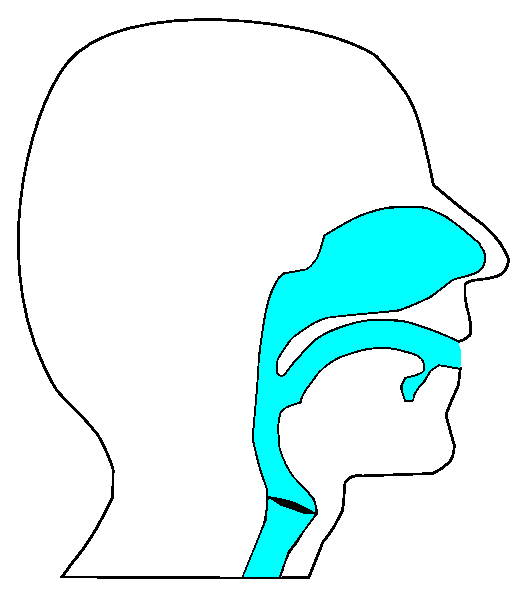
\includegraphics[width = .25\textwidth]{figures/Modell/kopfformanten.eps}}
node  [text width = 11.5cm] at (-15, -1)(text1) { \large Spektrum des Anregungssignals }
node  [text width = 11.5cm] at (-15, -1)(text1) { \large Spektrum des Anregungssignals }
node  [text width = 14cm] at (-0.3, -1)(text2) { \large Spektrum des aufgenommenen Signals }
node  [text width = 14cm] at (15.75, -1)(text3) { \large Spektrum des synthetisierten Signals }
node  [text width = 11.5cm] at (-15, -30)(text4) { \large \textbf{Sprachsignalanalyse} 
	
	Zur Parametrisierung des verwendeten Quelle-Filter-Modells m\"ussen reale Sprachsignale analysiert werden.
	
	Der Schwerpunkt liegt hierbei auf der Bestimmung der Filterparameter. Es werden prim\"ar Bandpassfilter 2. Ordnung eingesetzt. Die drei charakteristischen Parameter sind Mittenfrequenz, Bandbreite und Grundverst\"arkung.
	
	Die Mittenfrequenz wird als Formantfrequenz bezeichnet. Um diese zu bestimmen, wurden verschiedene Analysemethoden verwendet. Von der Software Praat wurde der fertig implementierte Burg-Algorithmus bereitgestellt, selbst nachprogrammiert wurde der Cepstrum-Algorithmus. 
	
	Dabei wird unter Annahme des Quelle-Filter-Modells eine Trennung von Quellsignal und \"Ubertragungsfunktion des Filters vorgenommen.
	}
node  [text width = 11.5cm] at (18, -23)(text5) { \large \textbf{Sprachsignalsynthese} 
	
Zur Synthese von Vokallauten wird ein periodisches breitbandiges Anregungssignal als Quelle verwendet. Die Signalformung wird mittels Bandpassfilter in Reihenschaltung realisiert.

Zur Synthese von Zischlauten wird ein Rauschgenerator als Quelle verwendet. Die Signalformung wird mittels Bandpassfilter in Parallelschaltung realisiert.

Bei der Lautkombination werden einzelne Laute mit einem Von-Hann-Fenster gefenstert und ineinander verschoben. Damit erreicht man neben verst\"andlichen Einzellauten auch eine gute Verst\"andlichkeit der ganzen Lautkombination.
}

node  [text width = 17cm] at (-1, -30)(text6) { \large \textbf{Syntheseergebnisse} 
	
	Implementiert wurden folgende Laute: Vokale, Diphtonge (/au/, /ei/, /eu/), stimmlose Frikative (/ch/, /f/, /s/, /sch/), stimmhafte Frikative (/w/), stimmhafte Plosive (/b/, /d/, /g/), stimmlose Plosive (/k/, /t/, /p/), Liquide (/l/, /r/) sowie Nasale (/m/, /n/).
	
	Allerdings k\"onnen stimmhafte Plosive nur in Verbindung mit einem darauffolgenden Vokal synthetisiert werden.
}
node  [text width = 25cm] at (5, -39)(text7) { \large \textbf{Quelle-Filter-Modell} 
	
Das Quelle-Filter-Modell versucht eine Zerlegung von Sprachsignalen in Anregungssignale und Filterstrukturen. Durch geeignete Wahl der Modellparameter soll eine m\"oglichst gute Modellierung des menschlichen Artikulationstrakts erreicht werden. 

}
node  [text width = 6cm] at (2, -19)(text6) { \large Anregungssignal}
node  [text width = 6cm] at (1, -7)(text7) { \large Vokaltrakt}
node  [text width = 6cm] at (11, -13)(text8) { \large Sprachsignal}
;


\draw
node at (-14, -37.11)[elipse](input) {\Huge {Quelle}} 
node at (-7, -37)[block] (filter) {\Huge {Filter}}
node  [text width = 15cm] at (18, -31)(Einleitung) { \includegraphics[width = .75\textwidth]{figures/Einleitung/von-kempelen.png}
	
	Von-Kempelen's Sprachautomat};



\draw [bigArrow](text6) to (5.005, -17);
\draw[->](text7) -- node {}(6, -9);
\draw[->](input) -- node {}(filter);
\draw[->](filter) -- node {\Large Ausgang}(1, -36.31);


\begin{scope}[scale = .3, xshift = \absheadposx-1500, yshift = 0]
% This file was created by matlab2tikz.
% Minimal pgfplots version: 1.3
%
%The latest updates can be retrieved from
%  http://www.mathworks.com/matlabcentral/fileexchange/22022-matlab2tikz
%where you can also make suggestions and rate matlab2tikz.
%
\begin{tikzpicture}

\begin{axis}[%
width=0.8\columnwidth,
%height=0.5\textwidth,
at={(0\textwidth,0\textwidth)},
scale only axis,
xmin=0,
xmax=3500,
xlabel={Frequenz f/Hz},
ymin=-80,
ymax=0,
ylabel={Betragsspektrum Anregungssignal in dB}
]
\addplot [color=blue,solid,forget plot]
  table[row sep=crcr]{%
-0.25	-7.41562743516466\\
0.25	0\\
0.75	-7.41562743516466\\
1.25	-81.1901665082484\\
1.75	-81.3921653550767\\
2.25	-81.448699705972\\
2.75	-81.4720991517142\\
3.25	-81.4833919712678\\
3.75	-81.489047732774\\
4.25	-81.4916237380112\\
4.75	-81.4923025315345\\
5.25	-81.4916939581271\\
5.75	-81.4901389798408\\
6.25	-81.4878405091311\\
6.75	-81.4849254598403\\
7.25	-81.4814764910319\\
7.75	-81.4775492708809\\
8.25	-81.4731823527754\\
8.75	-81.4684030708696\\
9.25	-81.4632311898836\\
9.75	-81.4576812368476\\
10.25	-81.4517640323387\\
10.75	-81.4454877207184\\
11.25	-81.4388584784056\\
11.75	-81.4318810102761\\
12.25	-81.4245589036544\\
12.75	-81.4168948847558\\
13.25	-81.4088910071109\\
13.75	-81.4005487918308\\
14.25	-81.3918693332621\\
14.75	-81.3828533794483\\
15.25	-81.3735013940114\\
15.75	-81.3638136041836\\
16.25	-81.3537900384084\\
16.75	-81.3434305559964\\
17.25	-81.3327348706828\\
17.75	-81.3217025694603\\
18.25	-81.3103331277243\\
18.75	-81.2986259215069\\
19.25	-81.2865802374166\\
19.75	-81.274195280733\\
20.25	-81.2614701820264\\
20.75	-81.2484040025812\\
21.25	-81.2349957388468\\
21.75	-81.2212443260934\\
22.25	-81.2071486414079\\
22.75	-81.1927075061502\\
23.25	-81.1779196879568\\
23.75	-81.1627839023611\\
24.25	-81.1472988140981\\
24.75	-81.1314630381387\\
25.25	-81.1152751404868\\
25.75	-81.0987336387888\\
26.25	-81.0818370027628\\
26.75	-81.064583654485\\
27.25	-81.0469719685448\\
27.75	-81.0290002720858\\
28.25	-81.0106668447463\\
28.75	-80.9919699185079\\
29.25	-80.9729076774674\\
29.75	-80.9534782575295\\
30.25	-80.9336797460359\\
30.75	-80.9135101813329\\
31.25	-80.8929675522786\\
31.75	-80.8720497976998\\
32.25	-80.8507548057952\\
32.75	-80.8290804134943\\
33.25	-80.8070244057661\\
33.75	-80.784584514886\\
34.25	-80.7617584196589\\
34.75	-80.7385437446006\\
35.25	-80.7149380590761\\
35.75	-80.6909388763998\\
36.25	-80.6665436528929\\
36.75	-80.6417497869008\\
37.25	-80.6165546177701\\
37.75	-80.5909554247851\\
38.25	-80.5649494260629\\
38.75	-80.538533777405\\
39.25	-80.5117055711101\\
39.75	-80.4844618347413\\
40.25	-80.4567995298489\\
40.75	-80.4287155506503\\
41.25	-80.4002067226633\\
41.75	-80.3712698012909\\
42.25	-80.3419014703593\\
42.75	-80.3120983406071\\
43.25	-80.2818569481188\\
43.75	-80.2511737527122\\
44.25	-80.2200451362661\\
44.75	-80.1884674009944\\
45.25	-80.1564367676623\\
45.75	-80.1239493737416\\
46.25	-80.0910012715053\\
46.75	-80.057588426057\\
47.25	-80.0237067132957\\
47.75	-79.9893519178102\\
48.25	-79.9545197307034\\
48.75	-79.919205747343\\
49.25	-79.8834054650336\\
49.75	-79.847114280614\\
50.25	-79.8103274879656\\
50.75	-79.7730402754423\\
51.25	-79.7352477232044\\
51.75	-79.6969448004678\\
52.25	-79.6581263626456\\
52.75	-79.6187871484061\\
53.25	-79.5789217766101\\
53.75	-79.5385247431506\\
54.25	-79.4975904176759\\
54.75	-79.456113040196\\
55.25	-79.4140867175659\\
55.75	-79.3715054198421\\
56.25	-79.3283629765067\\
56.75	-79.2846530725497\\
57.25	-79.240369244412\\
57.75	-79.1955048757717\\
58.25	-79.1500531931768\\
58.75	-79.1040072615103\\
59.25	-79.0573599792857\\
59.75	-79.0101040737608\\
60.25	-78.962232095865\\
60.75	-78.9137364149282\\
61.25	-78.864609213205\\
61.75	-78.8148424801841\\
62.25	-78.7644280066718\\
62.75	-78.7133573786379\\
63.25	-78.6616219708162\\
63.75	-78.6092129400458\\
64.25	-78.5561212183377\\
64.75	-78.5023375056588\\
65.25	-78.4478522624164\\
65.75	-78.3926557016268\\
66.25	-78.3367377807543\\
66.75	-78.2800881932056\\
67.25	-78.2226963594554\\
67.75	-78.1645514177933\\
68.25	-78.1056422146634\\
68.75	-78.0459572945829\\
69.25	-77.9854848896104\\
69.75	-77.9242129083464\\
70.25	-77.8621289244355\\
70.75	-77.7992201645469\\
71.25	-77.735473495801\\
71.75	-77.6708754126156\\
72.25	-77.6054120229368\\
72.75	-77.5390690338179\\
73.25	-77.4718317363141\\
73.75	-77.4036849896483\\
74.25	-77.3346132046116\\
74.75	-77.2646003261472\\
75.25	-77.1936298150727\\
75.75	-77.1216846288904\\
76.25	-77.0487472016281\\
76.75	-76.9747994226518\\
77.25	-76.8998226143879\\
77.75	-76.8237975088852\\
78.25	-76.7467042231453\\
78.75	-76.6685222331425\\
79.25	-76.5892303464485\\
79.75	-76.5088066733715\\
80.25	-76.427228596512\\
80.75	-76.3444727386307\\
81.25	-76.2605149287136\\
81.75	-76.1753301661144\\
82.25	-76.0888925826388\\
82.75	-76.0011754024311\\
83.25	-75.9121508995059\\
83.75	-75.8217903527589\\
84.25	-75.730063998275\\
84.75	-75.6369409787373\\
85.25	-75.5423892897222\\
85.75	-75.4463757226496\\
86.25	-75.3488658041342\\
86.75	-75.2498237314645\\
87.25	-75.1492123039073\\
87.75	-75.0469928495116\\
88.25	-74.9431251470541\\
88.75	-74.8375673427341\\
89.25	-74.7302758611904\\
89.75	-74.6212053103697\\
90.25	-74.5103083797318\\
90.75	-74.3975357312231\\
91.25	-74.2828358823981\\
91.75	-74.1661550809985\\
92.25	-74.0474371702354\\
92.75	-73.9266234439351\\
93.25	-73.8036524906236\\
93.75	-73.6784600255239\\
94.25	-73.5509787093278\\
94.75	-73.4211379524774\\
95.25	-73.2888637035476\\
95.75	-73.1540782201648\\
96.25	-73.0166998207006\\
96.75	-72.8766426148\\
97.25	-72.7338162105205\\
97.75	-72.588125395648\\
98.25	-72.4394697903992\\
98.75	-72.2877434683967\\
99.25	-72.1328345423935\\
99.75	-71.9746247107583\\
100.25	-71.8129887602074\\
100.75	-71.6477940196492\\
101.25	-71.4788997592982\\
101.75	-71.3061565283966\\
102.25	-71.1294054239096\\
102.75	-70.94847728146\\
103.25	-70.7631917784465\\
103.75	-70.5733564377675\\
104.25	-70.3787655187649\\
104.75	-70.1791987798835\\
105.25	-69.9744200950277\\
105.75	-69.7641759026194\\
106.25	-69.5481934628161\\
106.75	-69.3261788941206\\
107.25	-69.0978149555471\\
107.75	-68.8627585344327\\
108.25	-68.6206377926555\\
108.75	-68.3710489151758\\
109.25	-68.1135523941019\\
109.75	-67.8476687684638\\
110.25	-67.5728737240457\\
110.75	-67.2885924383213\\
111.25	-66.9941930319991\\
111.75	-66.6889789599865\\
112.25	-66.3721801397028\\
112.75	-66.0429425724884\\
113.25	-65.7003161633812\\
113.75	-65.3432403851965\\
114.25	-64.9705273653229\\
114.75	-64.5808419013843\\
115.25	-64.1726778442887\\
115.75	-63.7443302459664\\
116.25	-63.293862701554\\
116.75	-62.8190695220702\\
117.25	-62.3174329648587\\
117.75	-61.7860771740845\\
118.25	-61.2217237150111\\
118.75	-60.6206607917973\\
119.25	-59.9787544368518\\
119.75	-59.2915673289179\\
120.25	-58.5547408080414\\
120.75	-57.7650251675885\\
121.25	-56.9229779582567\\
121.75	-56.0403057230661\\
122.25	-55.1618340028153\\
122.75	-54.4435567222765\\
123.25	-54.5357674739217\\
123.75	-61.3215490850478\\
124.25	-41.0106321272808\\
124.75	-9.68818065345056\\
125.25	-4.4784450059893\\
125.75	-14.2571410420491\\
126.25	-49.1859409235374\\
126.75	-57.2370217121201\\
127.25	-54.3771381855127\\
127.75	-54.6605565518676\\
128.25	-55.4596561604291\\
128.75	-56.3540367232752\\
129.25	-57.2344026129006\\
129.75	-58.0691278800462\\
130.25	-58.8508343969718\\
130.75	-59.5804404859158\\
131.25	-60.2616482340092\\
131.75	-60.8988823492214\\
132.25	-61.4965021796139\\
132.75	-62.0585166859521\\
133.25	-62.5885050422284\\
133.75	-63.0896209203068\\
134.25	-63.5646285301766\\
134.75	-64.0159479947751\\
135.25	-64.4457005511976\\
135.75	-64.8557498434974\\
136.25	-65.2477381598309\\
136.75	-65.6231175971647\\
137.25	-65.9831765928733\\
137.75	-66.32906240803\\
138.25	-66.661800153804\\
138.75	-66.9823089017149\\
139.25	-67.2914153489693\\
139.75	-67.5898654391692\\
140.25	-67.8783342737095\\
140.75	-68.1574345926449\\
141.25	-68.427724055964\\
141.75	-68.6897115163519\\
142.25	-68.9438624416039\\
142.75	-69.1906036177982\\
143.25	-69.4303272421329\\
143.75	-69.6633944961289\\
144.25	-69.8901386749525\\
144.75	-70.1108679363218\\
145.25	-70.325867722329\\
145.75	-70.5354028991456\\
146.25	-70.7397196526397\\
146.75	-70.9390471721749\\
147.25	-71.1335991500511\\
147.75	-71.3235751200411\\
148.25	-71.509161655096\\
148.75	-71.6905334414718\\
149.25	-71.8678542441247\\
149.75	-72.0412777762117\\
150.25	-72.2109484838045\\
150.75	-72.3770022554707\\
151.25	-72.5395670651181\\
151.75	-72.6987635554411\\
152.25	-72.8547055683792\\
152.75	-73.0075006282158\\
153.25	-73.1572503822615\\
153.75	-73.3040510034767\\
154.25	-73.4479935588782\\
154.75	-73.5891643471311\\
155.25	-73.7276452083403\\
155.75	-73.8635138087179\\
156.25	-73.9968439025088\\
156.75	-74.1277055732968\\
157.25	-74.256165456588\\
157.75	-74.3822869453663\\
158.25	-74.5061303801406\\
158.75	-74.6277532248465\\
159.25	-74.7472102298308\\
159.75	-74.8645535830184\\
160.25	-74.979833050259\\
160.75	-75.0930961057509\\
161.25	-75.2043880533541\\
161.75	-75.3137521395283\\
162.25	-75.4212296585611\\
162.75	-75.5268600506932\\
163.25	-75.6306809936898\\
163.75	-75.7327284883579\\
164.25	-75.8330369384663\\
164.75	-75.9316392254852\\
165.25	-76.028566778522\\
165.75	-76.1238496398036\\
166.25	-76.2175165260216\\
166.75	-76.30959488583\\
167.25	-76.4001109537651\\
167.75	-76.4890898008292\\
168.25	-76.5765553819651\\
168.75	-76.6625305806268\\
169.25	-76.7470372506382\\
169.75	-76.8300962555112\\
170.25	-76.9117275053916\\
170.75	-76.9919499917713\\
171.25	-77.0707818201153\\
171.75	-77.1482402405215\\
172.25	-77.2243416765351\\
172.75	-77.2991017522234\\
173.25	-77.3725353176147\\
173.75	-77.4446564725885\\
174.25	-77.5154785893081\\
174.75	-77.5850143332698\\
175.25	-77.6532756830491\\
175.75	-77.7202739488044\\
176.25	-77.7860197896056\\
176.75	-77.8505232296452\\
177.25	-77.9137936733871\\
177.75	-77.9758399197001\\
178.25	-78.0366701750251\\
178.75	-78.0962920656184\\
179.25	-78.1547126489097\\
179.75	-78.2119384240127\\
180.25	-78.2679753414209\\
180.75	-78.3228288119202\\
181.25	-78.3765037147473\\
181.75	-78.4290044050187\\
182.25	-78.4803347204562\\
182.75	-78.5304979874296\\
183.25	-78.5794970263348\\
183.75	-78.627334156331\\
184.25	-78.6740111994448\\
184.75	-78.7195294840626\\
185.25	-78.7638898478221\\
185.75	-78.8070926399106\\
186.25	-78.8491377227845\\
186.75	-78.8900244733148\\
187.25	-78.9297517833693\\
187.75	-78.9683180598297\\
188.25	-79.005721224052\\
188.75	-79.0419587107757\\
189.25	-79.0770274664731\\
189.75	-79.1109239471487\\
190.25	-79.1436441155797\\
190.75	-79.1751834379967\\
191.25	-79.2055368802014\\
191.75	-79.2346989031132\\
192.25	-79.2626634577343\\
192.75	-79.2894239795363\\
193.25	-79.3149733822386\\
193.75	-79.3393040509841\\
194.25	-79.3624078348882\\
194.75	-79.3842760389484\\
195.25	-79.4048994152989\\
195.75	-79.4242681537865\\
196.25	-79.4423718718513\\
196.75	-79.4591996036859\\
197.25	-79.4747397886494\\
197.75	-79.4889802589052\\
198.25	-79.501908226257\\
198.75	-79.5135102681463\\
199.25	-79.5237723127739\\
199.75	-79.5326796233166\\
200.25	-79.5402167811814\\
200.75	-79.546367668263\\
201.25	-79.5511154481545\\
201.75	-79.5544425462515\\
202.25	-79.5563306286986\\
202.75	-79.5567605801116\\
203.25	-79.5557124800099\\
203.75	-79.5531655778863\\
204.25	-79.5490982668328\\
204.75	-79.5434880556411\\
205.25	-79.5363115392816\\
205.75	-79.5275443676614\\
206.25	-79.5171612125558\\
206.75	-79.5051357325936\\
207.25	-79.491440536166\\
207.75	-79.4760471421283\\
208.25	-79.4589259381369\\
208.75	-79.4400461364628\\
209.25	-79.419375727104\\
209.75	-79.3968814280018\\
210.25	-79.3725286321546\\
210.75	-79.3462813513984\\
211.25	-79.3181021566035\\
211.75	-79.2879521140182\\
212.25	-79.255790717461\\
212.75	-79.2215758160335\\
213.25	-79.1852635370023\\
213.75	-79.1468082034566\\
214.25	-79.1061622463148\\
214.75	-79.0632761102097\\
215.25	-79.0180981527375\\
215.75	-78.9705745364985\\
216.25	-78.9206491133077\\
216.75	-78.868263299881\\
217.25	-78.8133559442342\\
217.75	-78.7558631819523\\
218.25	-78.6957182813924\\
218.75	-78.6328514767851\\
219.25	-78.5671897880806\\
219.75	-78.4986568262606\\
220.25	-78.4271725826911\\
220.75	-78.3526532009209\\
221.25	-78.2750107291492\\
221.75	-78.1941528513763\\
222.25	-78.109982594998\\
222.75	-78.0223980123446\\
223.25	-77.9312918333417\\
223.75	-77.836551086115\\
224.25	-77.7380566819451\\
224.75	-77.6356829605174\\
225.25	-77.5292971908478\\
225.75	-77.4187590226546\\
226.25	-77.3039198822058\\
226.75	-77.1846223058345\\
227.25	-77.0606992033233\\
227.75	-76.9319730422203\\
228.25	-76.7982549428023\\
228.75	-76.6593436718274\\
229.25	-76.5150245213742\\
229.75	-76.3650680568732\\
230.25	-76.2092287158594\\
230.75	-76.0472432359063\\
231.25	-75.8788288865531\\
231.75	-75.7036814756763\\
232.25	-75.5214730955366\\
232.75	-75.3318495674607\\
233.25	-75.1344275365488\\
233.75	-74.9287911586615\\
234.25	-74.7144883108544\\
234.75	-74.4910262429574\\
235.25	-74.2578665715905\\
235.75	-74.014419497893\\
236.25	-73.760037105818\\
236.75	-73.4940055680406\\
237.25	-73.2155360502743\\
237.75	-72.9237540609247\\
238.25	-72.6176869404881\\
238.75	-72.2962491233707\\
239.25	-71.9582247346254\\
239.75	-71.602247009219\\
240.25	-71.2267739520397\\
240.75	-70.8300596164868\\
241.25	-70.4101204194374\\
241.75	-69.9646961395701\\
242.25	-69.4912058947825\\
242.75	-68.9867009545725\\
243.25	-68.4478197857607\\
243.75	-67.870758656185\\
244.25	-67.2512890268058\\
244.75	-66.5848945410221\\
245.25	-65.8672012914407\\
245.75	-65.0951352593431\\
246.25	-64.2699702126105\\
246.75	-63.405717974174\\
247.25	-62.5547271366347\\
247.75	-61.9016489359062\\
248.25	-62.2563846848249\\
248.75	-73.7138077242907\\
249.25	-44.7577160970782\\
249.75	-20.8045136000864\\
250.25	-17.6956897731283\\
250.75	-30.0803280728855\\
251.25	-61.6288843086609\\
251.75	-64.0422070698126\\
252.25	-62.1229535927486\\
252.75	-62.5409525712424\\
253.25	-63.3759609484212\\
253.75	-64.2827373213584\\
254.25	-65.1685842295773\\
254.75	-66.0066676034289\\
255.25	-66.7911492135524\\
255.75	-67.5234303156907\\
256.25	-68.2073218274884\\
256.75	-68.8472226580358\\
257.25	-69.4474219970945\\
257.75	-70.0118493949707\\
258.25	-70.5440087551461\\
258.75	-71.0469871534311\\
259.25	-71.5234917800531\\
259.75	-71.9758947851862\\
260.25	-72.4062774624152\\
260.75	-72.8164704349329\\
261.25	-73.2080888575607\\
261.75	-73.5825626723228\\
262.25	-73.9411623655747\\
262.75	-74.285020801576\\
263.25	-74.6151517077628\\
263.75	-74.932465335495\\
264.25	-75.2377817519038\\
264.75	-75.5318421496518\\
265.25	-75.8153184986294\\
265.75	-76.0888218090689\\
266.25	-76.3529092294268\\
266.75	-76.6080901639544\\
267.25	-76.8548315631272\\
267.75	-77.0935625139917\\
268.25	-77.3246782360505\\
268.75	-77.5485435707191\\
269.25	-77.7654960379284\\
269.75	-77.9758485215573\\
270.25	-78.17989163557\\
270.75	-78.3778958146252\\
271.25	-78.5701131661914\\
271.75	-78.7567791156228\\
272.25	-78.9381138709731\\
272.75	-79.1143237304306\\
273.25	-79.2856022519773\\
273.75	-79.4521313021223\\
274.25	-79.6140819982265\\
274.75	-79.7716155569656\\
275.25	-79.9248840598093\\
275.75	-80.0740311449544\\
276.25	-80.2191926339492\\
276.75	-80.3604971001868\\
277.25	-80.4980663855575\\
277.75	-80.6320160707766\\
278.25	-80.7624559042361\\
278.75	-80.8894901936545\\
279.25	-81.0132181642974\\
279.75	-81.1337342871072\\
280.25	-81.2511285797018\\
280.75	-81.3654868828668\\
281.25	-81.4768911148893\\
281.75	-81.5854195058056\\
282.25	-81.6911468134347\\
282.75	-81.794144522857\\
283.25	-81.8944810308316\\
283.75	-81.9922218164905\\
284.25	-82.0874295995113\\
284.75	-82.1801644868521\\
285.25	-82.2704841090246\\
285.75	-82.3584437467816\\
286.25	-82.4440964490188\\
286.75	-82.527493142609\\
287.25	-82.6086827348204\\
287.75	-82.6877122089084\\
288.25	-82.7646267134237\\
288.75	-82.8394696457182\\
289.25	-82.9122827300957\\
289.75	-82.9831060910151\\
290.25	-83.0519783217094\\
290.75	-83.118936548563\\
291.25	-83.1840164915514\\
291.75	-83.2472525210264\\
292.25	-83.3086777111073\\
292.75	-83.3683238899056\\
293.25	-83.4262216868134\\
293.75	-83.4824005770419\\
294.25	-83.5368889235986\\
294.75	-83.589714016867\\
295.25	-83.640902111956\\
295.75	-83.6904784639358\\
296.25	-83.7384673611192\\
296.75	-83.7848921564877\\
297.25	-83.8297752973875\\
297.75	-83.8731383535872\\
298.25	-83.9150020437983\\
298.75	-83.955386260746\\
299.25	-83.9943100948649\\
299.75	-84.0317918567005\\
300.25	-84.0678490980837\\
300.75	-84.1024986321375\\
301.25	-84.1357565521803\\
301.75	-84.16763824958\\
302.25	-84.198158430597\\
302.75	-84.227331132287\\
303.25	-84.2551697374762\\
303.75	-84.281686988873\\
304.25	-84.306895002339\\
304.75	-84.3308052793561\\
305.25	-84.35342871872\\
305.75	-84.3747756274922\\
306.25	-84.3948557312283\\
306.75	-84.4136781835113\\
307.25	-84.4312515748145\\
307.75	-84.4475839407033\\
308.25	-84.4626827694034\\
308.75	-84.4765550087468\\
309.25	-84.4892070725042\\
309.75	-84.5006448461336\\
310.25	-84.5108736919312\\
310.75	-84.5198984536085\\
311.25	-84.5277234603074\\
311.75	-84.5343525300515\\
312.25	-84.5397889726358\\
312.75	-84.5440355919569\\
313.25	-84.5470946878101\\
313.75	-84.548968057114\\
314.25	-84.5496569945932\\
314.75	-84.5491622929078\\
315.25	-84.5474842422177\\
315.75	-84.5446226291904\\
316.25	-84.5405767354316\\
316.75	-84.5353453353574\\
317.25	-84.528926693447\\
317.75	-84.5213185609296\\
318.25	-84.5125181718483\\
318.75	-84.5025222385014\\
319.25	-84.4913269462415\\
319.75	-84.4789279476246\\
320.25	-84.4653203558784\\
320.75	-84.4504987376732\\
321.25	-84.4344571051754\\
321.75	-84.4171889073509\\
322.25	-84.3986870204974\\
322.75	-84.3789437379718\\
323.25	-84.3579507590806\\
323.75	-84.3356991770963\\
324.25	-84.3121794663666\\
324.75	-84.2873814684664\\
325.25	-84.2612943773553\\
325.75	-84.2339067234896\\
326.25	-84.2052063568296\\
326.75	-84.1751804287005\\
327.25	-84.1438153724279\\
327.75	-84.111096882696\\
328.25	-84.0770098935501\\
328.75	-84.0415385549674\\
329.25	-84.0046662079144\\
329.75	-83.9663753578\\
330.25	-83.9266476462278\\
330.75	-83.8854638209418\\
331.25	-83.8428037038533\\
331.75	-83.7986461570259\\
332.25	-83.7529690464843\\
332.75	-83.7057492037061\\
333.25	-83.6569623846357\\
333.75	-83.6065832260571\\
334.25	-83.5545851991349\\
334.75	-83.5009405599303\\
335.25	-83.4456202966701\\
335.75	-83.3885940735354\\
336.25	-83.3298301707096\\
336.75	-83.2692954204087\\
337.25	-83.2069551385848\\
337.75	-83.1427730519675\\
338.25	-83.0767112200814\\
338.75	-83.0087299518341\\
339.25	-82.9387877162393\\
339.75	-82.8668410467921\\
340.25	-82.7928444389659\\
340.75	-82.7167502402533\\
341.25	-82.6385085321073\\
341.75	-82.5580670030731\\
342.25	-82.4753708123434\\
342.75	-82.390362442859\\
343.25	-82.3029815430142\\
343.75	-82.2131647559028\\
344.25	-82.1208455349318\\
344.75	-82.0259539445004\\
345.25	-81.9284164442883\\
345.75	-81.828155655531\\
346.25	-81.7250901074786\\
346.75	-81.6191339620011\\
347.25	-81.5101967140752\\
347.75	-81.3981828655991\\
348.25	-81.2829915696644\\
348.75	-81.1645162420473\\
349.25	-81.042644136262\\
349.75	-80.9172558780409\\
350.25	-80.7882249545427\\
350.75	-80.6554171529548\\
351.25	-80.5186899424064\\
351.75	-80.3778917922541\\
352.25	-80.232861418784\\
352.75	-80.0834269512172\\
353.25	-79.9294050065202\\
353.75	-79.7705996609215\\
354.25	-79.6068013041332\\
354.75	-79.437785360046\\
355.25	-79.263310855017\\
355.75	-79.0831188117236\\
356.25	-78.8969304428145\\
356.75	-78.7044451141185\\
357.25	-78.5053380418023\\
357.75	-78.2992576814297\\
358.25	-78.0858227590953\\
358.75	-77.8646188854078\\
359.25	-77.6351946816865\\
359.75	-77.3970573338787\\
360.25	-77.1496674728014\\
360.75	-76.892433258702\\
361.25	-76.6247035229678\\
361.75	-76.3457597891151\\
362.25	-76.0548069578531\\
362.75	-75.7509623958939\\
363.25	-75.4332431142231\\
363.75	-75.1005506583389\\
364.25	-74.7516532615078\\
364.75	-74.3851647367368\\
365.25	-73.9995195153861\\
365.75	-73.5929432063829\\
366.25	-73.1634181067769\\
366.75	-72.7086433626017\\
367.25	-72.2259902143277\\
367.75	-71.712454510722\\
368.25	-71.1646126347724\\
368.75	-70.5785958508475\\
369.25	-69.9501181747788\\
369.75	-69.2746397800082\\
370.25	-68.5478626476472\\
370.75	-67.7670541481547\\
371.25	-66.9345441081039\\
371.75	-66.0674592789135\\
372.25	-65.2280346981117\\
372.75	-64.6390104197747\\
373.25	-65.3392706163475\\
373.75	-89.6835413538922\\
374.25	-43.4287466677579\\
374.75	-24.2198566562981\\
375.25	-23.1521343839075\\
375.75	-38.5133989038265\\
376.25	-70.9211005846601\\
376.75	-66.2243711412388\\
377.25	-64.9736884228904\\
377.75	-65.5000467186619\\
378.25	-66.3627132260573\\
378.75	-67.2775908608371\\
379.25	-68.1663945311549\\
379.75	-69.0066299087751\\
380.25	-69.7939076198716\\
380.75	-70.5301064730153\\
381.25	-71.2191592515431\\
381.75	-71.8654527736015\\
382.25	-72.4732160821053\\
382.75	-73.0463050608569\\
383.25	-73.5881502674651\\
383.75	-74.1017709197105\\
384.25	-74.5898133176961\\
384.75	-75.0545956319166\\
385.25	-75.4981514389663\\
385.75	-75.9222690877165\\
386.25	-76.3285260883163\\
386.75	-76.7183186320452\\
387.25	-77.0928867109196\\
387.75	-77.4533354112257\\
388.25	-77.8006529468936\\
388.75	-78.1357259445438\\
389.25	-78.4593524239637\\
389.75	-78.7722528501091\\
390.25	-79.0750795714225\\
390.75	-79.368424906192\\
391.25	-79.6528280938773\\
391.75	-79.9287812910404\\
392.25	-80.1967347607266\\
392.75	-80.4571013788153\\
393.25	-80.7102605600705\\
393.75	-80.9565616895468\\
394.25	-81.1963271309837\\
394.75	-81.4298548722675\\
395.25	-81.6574208585104\\
395.75	-81.8792810554179\\
396.25	-82.0956732790693\\
396.75	-82.3068188228037\\
397.25	-82.5129239073514\\
397.75	-82.7141809765663\\
398.25	-82.9107698579025\\
398.75	-83.1028588041138\\
399.25	-83.2906054303649\\
399.75	-83.4741575590301\\
400.25	-83.6536539828208\\
400.75	-83.8292251554837\\
401.25	-84.0009938181288\\
401.75	-84.169075568223\\
402.25	-84.3335793774099\\
402.75	-84.4946080635611\\
403.25	-84.652258721815\\
403.75	-84.8066231187932\\
404.25	-84.9577880536944\\
404.75	-85.105835689545\\
405.25	-85.250843857509\\
405.75	-85.3928863368394\\
406.25	-85.5320331127688\\
406.75	-85.6683506143874\\
407.25	-85.8019019343408\\
407.75	-85.9327470319816\\
408.25	-86.0609429214481\\
408.75	-86.1865438459814\\
409.25	-86.3096014396723\\
409.75	-86.4301648776998\\
410.25	-86.5482810160257\\
410.75	-86.6639945214143\\
411.25	-86.7773479925585\\
411.75	-86.8883820730323\\
412.25	-86.9971355567052\\
412.75	-87.1036454862055\\
413.25	-87.2079472449773\\
413.75	-87.3100746433902\\
414.25	-87.4100599993687\\
414.75	-87.5079342139252\\
415.25	-87.6037268419769\\
415.75	-87.6974661587674\\
416.25	-87.7891792222137\\
416.75	-87.8788919314557\\
417.25	-87.9666290818578\\
417.75	-88.052414416712\\
418.25	-88.1362706758494\\
418.75	-88.2182196413624\\
419.25	-88.2982821806253\\
419.75	-88.3764782867795\\
420.25	-88.4528271168254\\
420.75	-88.5273470274987\\
421.25	-88.6000556090232\\
421.75	-88.670969716891\\
422.25	-88.7401055017687\\
422.75	-88.8074784376411\\
423.25	-88.8731033482838\\
423.75	-88.9369944321585\\
424.25	-88.9991652858112\\
424.75	-89.0596289258487\\
425.25	-89.118397809569\\
425.75	-89.1754838543076\\
426.25	-89.2308984555621\\
426.75	-89.2846525039519\\
427.25	-89.3367564010629\\
427.75	-89.3872200742348\\
428.25	-89.4360529903233\\
428.75	-89.483264168489\\
429.25	-89.5288621920504\\
429.75	-89.5728552194311\\
430.25	-89.615250994245\\
430.75	-89.6560568545393\\
431.25	-89.6952797412325\\
431.75	-89.7329262057695\\
432.25	-89.7690024170201\\
432.75	-89.8035141674386\\
433.25	-89.836466878518\\
433.75	-89.8678656055331\\
434.25	-89.8977150416205\\
434.75	-89.9260195211885\\
435.25	-89.95278302267\\
435.75	-89.9780091706476\\
436.25	-90.0017012373533\\
436.75	-90.023862143545\\
437.25	-90.0444944587705\\
437.75	-90.0636004010329\\
438.25	-90.0811818358684\\
438.75	-90.0972402748073\\
439.25	-90.1117768732671\\
439.75	-90.1247924278352\\
440.25	-90.136287372975\\
440.75	-90.1462617771327\\
441.25	-90.1547153382491\\
441.75	-90.1616473786703\\
442.25	-90.167056839448\\
442.75	-90.1709422740367\\
443.25	-90.1733018413533\\
443.75	-90.1741332982055\\
444.25	-90.173433991077\\
444.75	-90.1712008472447\\
445.25	-90.1674303652172\\
445.75	-90.1621186044745\\
446.25	-90.1552611744937\\
446.75	-90.1468532230258\\
447.25	-90.1368894236101\\
447.75	-90.1253639622911\\
448.25	-90.1122705235103\\
448.75	-90.0976022751419\\
449.25	-90.0813518526243\\
449.75	-90.0635113421657\\
450.25	-90.044072262965\\
450.75	-90.0230255484099\\
451.25	-90.000361526195\\
451.75	-89.9760698973135\\
452.25	-89.950139713848\\
452.75	-89.9225593555157\\
453.25	-89.8933165048762\\
453.75	-89.8623981211404\\
454.25	-89.8297904124934\\
454.75	-89.7954788068444\\
455.25	-89.759447920897\\
455.75	-89.7216815274503\\
456.25	-89.6821625208071\\
456.75	-89.6408728801679\\
457.25	-89.5977936308796\\
457.75	-89.5529048033916\\
458.25	-89.5061853897648\\
458.75	-89.4576132975605\\
459.25	-89.4071653009247\\
459.75	-89.3548169886695\\
460.25	-89.3005427091257\\
460.75	-89.2443155115341\\
461.25	-89.1861070837129\\
461.75	-89.1258876857135\\
462.25	-89.0636260791674\\
462.75	-88.9992894519655\\
463.25	-88.9328433379175\\
463.75	-88.8642515309811\\
464.25	-88.7934759936031\\
464.75	-88.7204767587072\\
465.25	-88.6452118247741\\
465.75	-88.5676370434306\\
466.25	-88.4877059989047\\
466.75	-88.4053698786051\\
467.25	-88.3205773340797\\
467.75	-88.2332743314307\\
468.25	-88.1434039902517\\
468.75	-88.0509064099933\\
469.25	-87.9557184825831\\
469.75	-87.857773689959\\
470.25	-87.7570018850505\\
470.75	-87.6533290545576\\
471.25	-87.5466770616846\\
471.75	-87.4369633667837\\
472.25	-87.3241007235741\\
472.75	-87.2079968483685\\
473.25	-87.0885540593715\\
473.75	-86.9656688827658\\
474.25	-86.83923162186\\
474.75	-86.7091258850952\\
475.25	-86.5752280681247\\
475.75	-86.4374067845386\\
476.25	-86.2955222390366\\
476.75	-86.1494255359842\\
477.25	-85.998957915242\\
477.75	-85.843949905984\\
478.25	-85.6842203877949\\
478.75	-85.5195755467103\\
479.25	-85.3498077119167\\
479.75	-85.1746940565366\\
480.25	-84.9939951432281\\
480.75	-84.807453292097\\
481.25	-84.6147907445919\\
481.75	-84.4157075924681\\
482.25	-84.2098794354108\\
482.75	-83.9969547242966\\
483.25	-83.7765517391034\\
483.75	-83.5482551408296\\
484.25	-83.3116120250769\\
484.75	-83.0661273907311\\
485.25	-82.8112589198152\\
485.75	-82.5464109434495\\
486.25	-82.2709274430156\\
486.75	-81.9840839041448\\
487.25	-81.6850778028989\\
487.75	-81.3730174573497\\
488.25	-81.0469089227426\\
488.75	-80.7056405442662\\
489.25	-80.3479647095591\\
489.75	-79.9724762685984\\
490.25	-79.5775870246565\\
490.75	-79.1614956761425\\
491.25	-78.7221526691574\\
491.75	-78.2572197393901\\
492.25	-77.7640247653687\\
492.75	-77.2395145358732\\
493.25	-76.6802124967209\\
493.75	-76.0821985299373\\
494.25	-75.4411505147569\\
494.75	-74.7525406848747\\
495.25	-74.012211027563\\
495.75	-73.2178977042146\\
496.25	-72.3732715656541\\
496.75	-71.499316054111\\
497.25	-70.6705348763759\\
497.75	-70.158433865935\\
498.25	-71.3268475648515\\
498.75	-77.6482935579926\\
499.25	-44.3373145142601\\
499.75	-28.762421375015\\
500.25	-29.7144940963239\\
500.75	-48.6511137204751\\
501.25	-90.2061805073934\\
501.75	-71.2261289203597\\
502.25	-70.4732655765049\\
502.75	-71.0817018772116\\
503.25	-71.9572080731302\\
503.75	-72.866719326018\\
504.25	-73.7447334237418\\
504.75	-74.5727785285014\\
505.25	-75.3478723155033\\
505.75	-76.0723927177966\\
506.25	-76.7504279783967\\
506.75	-77.3863854821556\\
507.25	-77.9844631007319\\
507.75	-78.5484683636348\\
508.25	-79.0817807952755\\
508.75	-79.5873717714483\\
509.25	-80.0678450105807\\
509.75	-80.5254817621094\\
510.25	-80.9622840399175\\
510.75	-81.3800134263516\\
511.25	-81.7802248400254\\
511.75	-82.1642954626405\\
512.25	-82.5334493272972\\
512.75	-82.8887781510581\\
513.25	-83.2312589751682\\
513.75	-83.5617691178045\\
514.25	-83.8810988749287\\
514.75	-84.1899623373362\\
515.25	-84.4890066314935\\
515.75	-84.7788198396564\\
516.25	-85.0599378109303\\
516.75	-85.3328500385088\\
517.25	-85.5980047483001\\
517.75	-85.8558133194487\\
518.25	-86.1066541370125\\
518.75	-86.3508759603992\\
519.25	-86.588800877523\\
519.75	-86.8207269033648\\
520.25	-87.0469302723304\\
520.75	-87.2676674661339\\
521.25	-87.4831770125241\\
521.75	-87.6936810848929\\
522.25	-87.899386928344\\
522.75	-88.1004881341138\\
523.25	-88.2971657811044\\
523.75	-88.4895894606611\\
524.25	-88.6779181985186\\
524.75	-88.8623012859458\\
525.25	-89.0428790305339\\
525.75	-89.2197834356946\\
526.25	-89.3931388167801\\
526.75	-89.5630623607426\\
527.25	-89.7296646353722\\
527.75	-89.8930500534406\\
528.25	-90.0533172964174\\
528.75	-90.2105597018798\\
529.25	-90.3648656182653\\
529.75	-90.5163187301831\\
530.25	-90.6649983571529\\
530.75	-90.8109797283052\\
531.25	-90.9543342353153\\
531.75	-91.0951296655885\\
532.25	-91.2334304174969\\
532.75	-91.3692976992925\\
533.25	-91.502789713135\\
533.75	-91.6339618255535\\
534.25	-91.7628667254858\\
534.75	-91.8895545709796\\
535.25	-92.0140731254852\\
535.75	-92.13646788461\\
536.25	-92.2567821941134\\
536.75	-92.3750573598367\\
537.25	-92.4913327502311\\
537.75	-92.605645892019\\
538.25	-92.7180325595882\\
538.75	-92.8285268585219\\
539.25	-92.9371613037581\\
539.75	-93.0439668927588\\
540.25	-93.1489731740542\\
540.75	-93.2522083115043\\
541.25	-93.3536991445719\\
541.75	-93.453471244903\\
542.25	-93.5515489694586\\
542.75	-93.6479555104504\\
543.25	-93.7427129422738\\
543.75	-93.8358422656722\\
544.25	-93.9273634492779\\
544.75	-94.0172954687372\\
545.25	-94.1056563435487\\
545.75	-94.1924631717701\\
546.25	-94.277732162734\\
546.75	-94.3614786678782\\
547.25	-94.443717209824\\
547.75	-94.5244615097945\\
548.25	-94.6037245134781\\
548.75	-94.6815184154217\\
549.25	-94.7578546820433\\
549.75	-94.8327440733442\\
550.25	-94.9061966633727\\
550.75	-94.9782218595407\\
551.25	-95.0488284208238\\
551.75	-95.1180244749126\\
552.25	-95.1858175343779\\
552.75	-95.2522145118879\\
553.25	-95.3172217345247\\
553.75	-95.3808449572414\\
554.25	-95.4430893755102\\
554.75	-95.5039596371788\\
555.25	-95.5634598535838\\
555.75	-95.6215936099455\\
556.25	-95.6783639750675\\
556.75	-95.7337735103814\\
557.25	-95.7878242783421\\
557.75	-95.8405178502085\\
558.25	-95.8918553132215\\
558.75	-95.9418372772011\\
559.25	-95.9904638805769\\
559.75	-96.0377347958637\\
560.25	-96.0836492345962\\
560.75	-96.128205951733\\
561.25	-96.1714032495393\\
561.75	-96.2132389809616\\
562.25	-96.2537105524684\\
562.75	-96.2928149264178\\
563.25	-96.330548622905\\
563.75	-96.3669077211082\\
564.25	-96.4018878601312\\
564.75	-96.4354842393558\\
565.25	-96.4676916182666\\
565.75	-96.4985043157754\\
566.25	-96.5279162090264\\
566.75	-96.5559207316883\\
567.25	-96.5825108716214\\
567.75	-96.6076791681648\\
568.25	-96.6314177086968\\
568.75	-96.6537181247024\\
569.25	-96.6745715872273\\
569.75	-96.6939688017245\\
570.25	-96.7119000022554\\
570.75	-96.7283549450472\\
571.25	-96.7433229013626\\
571.75	-96.756792649658\\
572.25	-96.7687524670133\\
572.75	-96.7791901197747\\
573.25	-96.7880928534053\\
573.75	-96.7954473814797\\
574.25	-96.8012398738084\\
574.75	-96.805455943605\\
575.25	-96.8080806337058\\
575.75	-96.8090984017339\\
576.25	-96.808493104192\\
576.75	-96.8062479794004\\
577.25	-96.8023456292261\\
577.75	-96.7967679995316\\
578.25	-96.7894963592589\\
578.75	-96.7805112780874\\
579.25	-96.7697926025488\\
579.75	-96.7573194305391\\
580.25	-96.7430700840899\\
580.75	-96.7270220803202\\
581.25	-96.7091521004278\\
581.75	-96.6894359566003\\
582.25	-96.6678485567109\\
582.75	-96.6443638666383\\
583.25	-96.6189548700614\\
583.75	-96.5915935255294\\
584.25	-96.5622507206519\\
584.75	-96.5308962231647\\
585.25	-96.4974986286669\\
585.75	-96.4620253047806\\
586.25	-96.4244423314647\\
586.75	-96.3847144371887\\
587.25	-96.3428049306594\\
587.75	-96.2986756277406\\
588.25	-96.2522867732041\\
588.75	-96.2035969568769\\
589.25	-96.1525630237618\\
589.75	-96.0991399775945\\
590.25	-96.0432808773329\\
590.75	-95.9849367259453\\
591.25	-95.924056350858\\
591.75	-95.8605862753239\\
592.25	-95.7944705799048\\
592.75	-95.7256507531956\\
593.25	-95.6540655307896\\
593.75	-95.5796507213944\\
594.25	-95.5023390189065\\
594.75	-95.4220597990747\\
595.25	-95.3387388992675\\
595.75	-95.2522983796624\\
596.25	-95.1626562639942\\
596.75	-95.0697262577667\\
597.25	-94.9734174415747\\
597.75	-94.8736339369028\\
598.25	-94.7702745414321\\
598.75	-94.6632323305027\\
599.25	-94.5523942209441\\
599.75	-94.4376404929937\\
600.25	-94.3188442654229\\
600.75	-94.1958709183538\\
601.25	-94.0685774574403\\
601.75	-93.936811812208\\
602.25	-93.8004120603001\\
602.75	-93.6592055681264\\
603.25	-93.5130080370189\\
603.75	-93.3616224422648\\
604.25	-93.204837850447\\
604.75	-93.0424280981446\\
605.25	-92.8741503122876\\
605.75	-92.6997432491537\\
606.25	-92.5189254250512\\
606.75	-92.3313930070434\\
607.25	-92.1368174264051\\
607.75	-91.9348426707207\\
608.25	-91.7250822023311\\
608.75	-91.5071154409058\\
609.25	-91.2804837358833\\
609.75	-91.0446857398457\\
610.25	-90.7991720760571\\
610.75	-90.5433391715577\\
611.25	-90.2765221006234\\
611.75	-89.9979862509375\\
612.25	-89.7069175854185\\
612.75	-89.4024112251491\\
613.25	-89.0834580223149\\
613.75	-88.748928726382\\
614.25	-88.3975552735973\\
614.75	-88.0279086552183\\
615.25	-87.6383727582639\\
615.75	-87.2271135568779\\
616.25	-86.792043133201\\
616.75	-86.3307783733092\\
617.25	-85.8405951330012\\
617.75	-85.3183808816353\\
618.25	-84.760593810674\\
618.75	-84.1632475547102\\
619.25	-83.5219661370452\\
619.75	-82.8322138813402\\
620.25	-82.0899544343199\\
620.75	-81.2933911317947\\
621.25	-80.447606583546\\
621.75	-79.5778044778427\\
622.25	-78.7724607377377\\
622.75	-78.3619383751707\\
623.25	-80.1608897650982\\
623.75	-78.8329212641084\\
624.25	-47.0235950251601\\
624.75	-34.4618623687474\\
625.25	-37.4518177965979\\
625.75	-61.0255841534382\\
626.25	-92.2101410330652\\
626.75	-79.167059569396\\
627.25	-78.7803143583308\\
627.75	-79.4576888680126\\
628.25	-80.347694006965\\
628.75	-81.2570624012158\\
629.25	-82.1305946145544\\
629.75	-82.9530752474308\\
630.25	-83.7226374236786\\
630.75	-84.4420294203725\\
631.25	-85.1154311599724\\
631.75	-85.7472359238561\\
632.25	-86.3415900364924\\
632.75	-86.9022398751451\\
633.25	-87.4325054225358\\
633.75	-87.9353042747803\\
634.25	-88.4131932514867\\
634.75	-88.8684134324575\\
635.25	-89.3029327538875\\
635.75	-89.7184840388652\\
636.25	-90.1165980058899\\
636.75	-90.4986315095829\\
637.25	-90.8657915331966\\
637.75	-91.2191555143918\\
638.25	-91.5596885590335\\
638.75	-91.8882580370457\\
639.25	-92.2056459851321\\
639.75	-92.5125596747701\\
640.25	-92.8096406447043\\
640.75	-93.0974724463761\\
641.25	-93.3765873081149\\
641.75	-93.6474718885249\\
642.25	-93.9105722603051\\
642.75	-94.166298241799\\
643.25	-94.4150271738688\\
643.75	-94.6571072235415\\
644.25	-94.892860282592\\
644.75	-95.1225845182721\\
645.25	-95.3465566243845\\
645.75	-95.5650338134044\\
646.25	-95.7782555841407\\
646.75	-95.9864452942756\\
647.25	-96.1898115627874\\
647.75	-96.3885495236415\\
648.25	-96.582841949127\\
648.75	-96.7728602585844\\
649.25	-96.9587654262064\\
649.75	-97.1407087996429\\
650.25	-97.3188328396739\\
650.75	-97.4932717898224\\
651.25	-97.6641522836676\\
651.75	-97.8315938966473\\
652.25	-97.9957096482524\\
652.75	-98.1566064598778\\
653.25	-98.3143855728722\\
653.75	-98.4691429308537\\
654.25	-98.6209695298802\\
654.75	-98.7699517396119\\
655.25	-98.9161715983058\\
655.75	-99.0597070841223\\
656.25	-99.2006323649799\\
656.75	-99.3390180289368\\
657.25	-99.4749312968852\\
657.75	-99.6084362191305\\
658.25	-99.7395938573017\\
658.75	-99.8684624528535\\
659.25	-99.9950975833245\\
659.75	-100.119552307406\\
660.25	-100.24187729969\\
660.75	-100.362120976048\\
661.25	-100.480329610315\\
661.75	-100.596547443018\\
662.25	-100.71081678274\\
662.75	-100.823178100817\\
663.25	-100.933670119625\\
663.75	-101.042329895254\\
664.25	-101.149192894761\\
664.75	-101.254293068481\\
665.25	-101.357662917796\\
665.75	-101.459333558591\\
666.25	-101.5593347808\\
666.75	-101.657695104255\\
667.25	-101.754441831119\\
667.75	-101.849601095111\\
668.25	-101.943197907784\\
668.75	-102.03525620199\\
669.25	-102.125798872763\\
669.75	-102.214847815771\\
670.25	-102.302423963479\\
670.75	-102.38854731919\\
671.25	-102.473236989059\\
671.75	-102.556511212242\\
672.25	-102.638387389275\\
672.75	-102.718882108747\\
673.25	-102.798011172464\\
673.75	-102.875789619062\\
674.25	-102.952231746261\\
674.75	-103.027351131776\\
675.25	-103.101160652976\\
675.75	-103.173672505353\\
676.25	-103.244898219851\\
676.75	-103.314848679142\\
677.25	-103.38353413286\\
677.75	-103.450964211859\\
678.25	-103.517147941573\\
678.75	-103.582093754442\\
679.25	-103.645809501531\\
679.75	-103.708302463292\\
680.25	-103.769579359589\\
680.75	-103.829646358929\\
681.25	-103.888509086996\\
681.75	-103.946172634476\\
682.25	-104.002641564188\\
682.75	-104.057919917597\\
683.25	-104.112011220658\\
683.75	-104.164918489049\\
684.25	-104.2166442328\\
684.75	-104.267190460345\\
685.25	-104.316558681979\\
685.75	-104.364749912741\\
686.25	-104.41176467477\\
686.75	-104.457602999079\\
687.25	-104.50226442679\\
687.75	-104.545748009845\\
688.25	-104.588052311165\\
688.75	-104.629175404269\\
689.25	-104.66911487237\\
689.75	-104.707867806937\\
690.25	-104.745430805703\\
690.75	-104.781799970142\\
691.25	-104.816970902391\\
691.75	-104.850938701646\\
692.25	-104.883697959912\\
692.75	-104.915242757312\\
693.25	-104.945566656688\\
693.75	-104.974662697677\\
694.25	-105.002523390136\\
694.75	-105.029140706972\\
695.25	-105.054506076294\\
695.75	-105.078610372915\\
696.25	-105.101443909153\\
696.75	-105.12299642492\\
697.25	-105.143257077072\\
697.75	-105.162214427974\\
698.25	-105.179856433274\\
698.75	-105.196170428823\\
699.25	-105.211143116721\\
699.75	-105.224760550454\\
700.25	-105.237008119031\\
700.75	-105.24787053016\\
701.25	-105.257331792296\\
701.75	-105.265375195616\\
702.25	-105.27198329178\\
702.75	-105.27713787244\\
703.25	-105.28081994644\\
703.75	-105.283009715595\\
704.25	-105.283686548993\\
704.75	-105.282828955719\\
705.25	-105.280414555886\\
705.75	-105.276420049906\\
706.25	-105.270821185839\\
706.75	-105.263592724723\\
707.25	-105.254708403741\\
707.75	-105.244140897088\\
708.25	-105.231861774334\\
708.75	-105.217841456203\\
709.25	-105.20204916744\\
709.75	-105.184452886703\\
710.25	-105.165019293162\\
710.75	-105.143713709587\\
711.25	-105.120500041663\\
711.75	-105.09534071327\\
712.25	-105.068196597324\\
712.75	-105.039026941935\\
713.25	-105.007789291432\\
713.75	-104.974439401872\\
714.25	-104.938931150564\\
714.75	-104.901216439101\\
715.25	-104.861245089383\\
715.75	-104.818964731949\\
716.25	-104.774320686061\\
716.75	-104.727255830697\\
717.25	-104.677710465687\\
717.75	-104.625622162121\\
718.25	-104.570925600945\\
718.75	-104.513552398733\\
719.25	-104.453430919334\\
719.75	-104.390486070065\\
720.25	-104.324639080905\\
720.75	-104.255807265\\
721.25	-104.18390375857\\
721.75	-104.108837238067\\
722.25	-104.030511612253\\
722.75	-103.948825686411\\
723.25	-103.86367279576\\
723.75	-103.774940404596\\
724.25	-103.682509667318\\
724.75	-103.586254946957\\
725.25	-103.486043286241\\
725.75	-103.381733825559\\
726.25	-103.27317716133\\
726.75	-103.16021463746\\
727.25	-103.042677561416\\
727.75	-102.920386335204\\
728.25	-102.793149490098\\
728.75	-102.66076261221\\
729.25	-102.523007143925\\
729.75	-102.379649043925\\
730.25	-102.230437285489\\
730.75	-102.075102169565\\
731.25	-101.91335342488\\
731.75	-101.744878062635\\
732.25	-101.569337947426\\
732.75	-101.386367039086\\
733.25	-101.195568251618\\
733.75	-100.996509865225\\
734.25	-100.78872141487\\
734.75	-100.571688963761\\
735.25	-100.344849651565\\
735.75	-100.10758538463\\
736.25	-99.8592155078345\\
736.75	-99.598988264129\\
737.25	-99.3260708068015\\
737.75	-99.0395374802993\\
738.25	-98.7383560266856\\
738.75	-98.4213713067201\\
739.25	-98.0872860489761\\
739.75	-97.7346380636722\\
740.25	-97.3617732961858\\
740.75	-96.9668140842028\\
741.25	-96.5476220990113\\
741.75	-96.1017558591172\\
742.25	-95.6264237505212\\
742.75	-95.1184359235932\\
743.25	-94.5741639241702\\
743.75	-93.9895292652943\\
744.25	-93.3600704747794\\
744.75	-92.6812055341012\\
745.25	-91.9489756156593\\
745.75	-91.1620117679711\\
746.25	-90.3268220506711\\
746.75	-89.4731156036043\\
747.25	-88.7050417123922\\
747.75	-88.4235494751142\\
748.25	-91.0838119208496\\
748.75	-83.9967275786275\\
749.25	-49.2683101103904\\
749.75	-39.3365563346292\\
750.25	-44.4208560746684\\
750.75	-75.081572029985\\
751.25	-96.5272878415573\\
751.75	-89.2219988397406\\
752.25	-89.1134485756439\\
752.75	-89.8546860002571\\
753.25	-90.766789598445\\
753.75	-91.6872083778077\\
754.25	-92.5688476958325\\
754.75	-93.3990180299161\\
755.25	-94.1766696397302\\
755.75	-94.9047794212764\\
756.25	-95.5875430615579\\
756.75	-96.2292948359366\\
757.25	-96.8341006493496\\
757.75	-97.4056258062173\\
758.25	-97.9471161680363\\
758.75	-98.4614243480001\\
759.25	-98.9510513098939\\
759.75	-99.4181905712055\\
760.25	-99.8647697329567\\
760.75	-100.29248745646\\
761.25	-100.702845523493\\
761.75	-101.097176259571\\
762.25	-101.47666583699\\
762.75	-101.842374025428\\
763.25	-102.195250928289\\
763.75	-102.536151182798\\
764.25	-102.865846034434\\
764.75	-103.185033632091\\
765.25	-103.494347833083\\
765.75	-103.794365758282\\
766.25	-104.085614296535\\
766.75	-104.368575723261\\
767.25	-104.643692570204\\
767.75	-104.911371859928\\
768.25	-105.171988799846\\
768.75	-105.42589001477\\
769.25	-105.67339638429\\
769.75	-105.914805540519\\
770.25	-106.1503940732\\
770.75	-106.380419481673\\
771.25	-106.605121907431\\
771.75	-106.824725675745\\
772.25	-107.039440670849\\
772.75	-107.249463565468\\
773.25	-107.454978922676\\
773.75	-107.65616018549\\
774.25	-107.853170567478\\
774.75	-108.046163855994\\
775.25	-108.235285137946\\
775.75	-108.420671456845\\
776.25	-108.602452408784\\
776.75	-108.780750683868\\
777.25	-108.955682559009\\
777.75	-109.127358347189\\
778.25	-109.295882807614\\
778.75	-109.461355520854\\
779.25	-109.623871232365\\
779.75	-109.783520167605\\
780.25	-109.940388321357\\
780.75	-110.094557723953\\
781.25	-110.246106686312\\
781.75	-110.395110025971\\
782.25	-110.541639275679\\
782.75	-110.685762876301\\
783.25	-110.827546355243\\
783.75	-110.967052491811\\
784.25	-111.104341470533\\
784.75	-111.239471023545\\
785.25	-111.372496562927\\
785.75	-111.503471303772\\
786.25	-111.632446378896\\
786.75	-111.759470945614\\
787.25	-111.88459228569\\
787.75	-112.007855898079\\
788.25	-112.129305586329\\
788.75	-112.248983539852\\
789.25	-112.366930410187\\
789.75	-112.483185382463\\
790.25	-112.5977862424\\
790.75	-112.710769439194\\
791.25	-112.822170144568\\
791.75	-112.932022308312\\
792.25	-113.040358710463\\
792.75	-113.147211010492\\
793.25	-113.25260979355\\
793.75	-113.35658461411\\
794.25	-113.459164037077\\
794.75	-113.560375676653\\
795.25	-113.660246232909\\
795.75	-113.758801526435\\
796.25	-113.856066531058\\
796.75	-113.952065404728\\
797.25	-114.046821518811\\
797.75	-114.14035748578\\
798.25	-114.232695185368\\
798.75	-114.323855789485\\
799.25	-114.413859785653\\
799.75	-114.502726999343\\
800.25	-114.59047661508\\
800.75	-114.677127196496\\
801.25	-114.762696705301\\
801.75	-114.847202519306\\
802.25	-114.93066144953\\
802.75	-115.013089756375\\
803.25	-115.094503165008\\
803.75	-115.174916879957\\
804.25	-115.254345598926\\
804.75	-115.33280352583\\
805.25	-115.410304383336\\
805.75	-115.48686142452\\
806.25	-115.562487444029\\
806.75	-115.637194788626\\
807.25	-115.710995367095\\
807.75	-115.783900659724\\
808.25	-115.855921727088\\
808.75	-115.927069218429\\
809.25	-115.997353379582\\
809.75	-116.066784060158\\
810.25	-116.135370720669\\
810.75	-116.203122438869\\
811.25	-116.270047915759\\
811.75	-116.336155481215\\
812.25	-116.401453099101\\
812.75	-116.46594837205\\
813.25	-116.529648545789\\
813.75	-116.59256051307\\
814.25	-116.654690817226\\
814.75	-116.716045655331\\
815.25	-116.77663088091\\
815.75	-116.836452006385\\
816.25	-116.895514204974\\
816.75	-116.953822312391\\
817.25	-117.011380827952\\
817.75	-117.068193915419\\
818.25	-117.12426540345\\
818.75	-117.179598785552\\
819.25	-117.2341972197\\
819.75	-117.288063527551\\
820.25	-117.341200193153\\
820.75	-117.393609361271\\
821.25	-117.445292835273\\
821.75	-117.496252074512\\
822.25	-117.546488191264\\
822.75	-117.596001947126\\
823.25	-117.644793748982\\
823.75	-117.692863644316\\
824.25	-117.740211316068\\
824.75	-117.786836076871\\
825.25	-117.832736862639\\
825.75	-117.87791222559\\
826.25	-117.922360326511\\
826.75	-117.966078926384\\
827.25	-118.009065377205\\
827.75	-118.051316612042\\
828.25	-118.092829134291\\
828.75	-118.13359900588\\
829.25	-118.173621834802\\
829.75	-118.212892761362\\
830.25	-118.251406443523\\
830.75	-118.289157041054\\
831.25	-118.326138198473\\
831.75	-118.362343026653\\
832.25	-118.397764083063\\
832.75	-118.432393350505\\
833.25	-118.466222214207\\
833.75	-118.499241437213\\
834.25	-118.531441133926\\
834.75	-118.562810741589\\
835.25	-118.593338989646\\
835.75	-118.623013866734\\
836.25	-118.651822585142\\
836.75	-118.679751542594\\
837.25	-118.706786280934\\
837.75	-118.732911441706\\
838.25	-118.758110718148\\
838.75	-118.782366803445\\
839.25	-118.805661334772\\
839.75	-118.82797483282\\
840.25	-118.849286636419\\
840.75	-118.869574831757\\
841.25	-118.888816175553\\
841.75	-118.90698601197\\
842.25	-118.924058182286\\
842.75	-118.940004926716\\
843.25	-118.954796777756\\
843.75	-118.968402443913\\
844.25	-118.980788683174\\
844.75	-118.991920164698\\
845.25	-119.001759317895\\
845.75	-119.010266167332\\
846.25	-119.017398151744\\
846.75	-119.023109925781\\
847.25	-119.027353142173\\
847.75	-119.030076212099\\
848.25	-119.03122404148\\
848.75	-119.030737739822\\
849.25	-119.028554298792\\
849.75	-119.024606236392\\
850.25	-119.018821202577\\
850.75	-119.011121541316\\
851.25	-119.001423803356\\
851.75	-118.989638203282\\
852.25	-118.975668013016\\
852.75	-118.95940888325\\
853.25	-118.94074808243\\
853.75	-118.919563641447\\
854.25	-118.895723390252\\
854.75	-118.869083869939\\
855.25	-118.839489101477\\
855.75	-118.806769188279\\
856.25	-118.770738726288\\
856.75	-118.731194989756\\
857.25	-118.687915855258\\
857.75	-118.640657419003\\
858.25	-118.589151253515\\
858.75	-118.533101239043\\
859.25	-118.472179891033\\
859.75	-118.406024089104\\
860.25	-118.334230091513\\
860.75	-118.256347694329\\
861.25	-118.171873361303\\
861.75	-118.080242112349\\
862.25	-117.980817906904\\
862.75	-117.872882197248\\
863.25	-117.755620249604\\
863.75	-117.628104734878\\
864.25	-117.489275975518\\
864.75	-117.337918098079\\
865.25	-117.172630188369\\
865.75	-116.991791395161\\
866.25	-116.793518826837\\
866.75	-116.575617144412\\
867.25	-116.335519231669\\
867.75	-116.070218807179\\
868.25	-115.776199686409\\
868.75	-115.449375813524\\
869.25	-115.085079039767\\
869.75	-114.678188305957\\
870.25	-114.223640688469\\
870.75	-113.717971021111\\
871.25	-113.163761597288\\
871.75	-112.583167447057\\
872.25	-112.06473704884\\
872.75	-111.972147793107\\
873.25	-114.626579300799\\
873.75	-107.464948663147\\
874.25	-48.5036809204703\\
874.75	-40.9512869888926\\
875.25	-48.2308193848466\\
875.75	-104.274754289246\\
876.25	-130.975723484637\\
876.75	-120.244389671864\\
877.25	-120.413821707411\\
877.75	-121.816400280516\\
878.25	-123.609967546756\\
878.75	-125.614482127794\\
879.25	-127.812248411327\\
879.75	-130.260476722011\\
880.25	-133.092526666309\\
880.75	-136.587968051075\\
881.25	-141.452331991674\\
881.75	-150.663962927821\\
882.25	-154.06444740676\\
882.75	-144.054505313114\\
883.25	-139.91248460896\\
883.75	-137.371530148058\\
884.25	-135.584389160999\\
884.75	-134.232934461399\\
885.25	-133.163201865322\\
885.75	-132.289149276556\\
886.25	-131.557959683341\\
886.75	-130.934983735139\\
887.25	-130.396333577732\\
887.75	-129.924892910789\\
888.25	-129.508012911201\\
888.75	-129.136106688971\\
889.25	-128.801752881925\\
889.75	-128.499102522784\\
890.25	-128.223474219668\\
890.75	-127.971070451216\\
891.25	-127.738774140664\\
891.75	-127.523999849917\\
892.25	-127.324582995824\\
892.75	-127.138696074442\\
893.25	-126.964784418117\\
893.75	-126.801516307517\\
894.25	-126.647743788399\\
894.75	-126.502471575914\\
895.25	-126.364832142945\\
895.75	-126.234065588934\\
896.25	-126.10950324155\\
896.75	-125.990554199972\\
897.25	-125.876694216427\\
897.75	-125.767456451085\\
898.25	-125.662423738824\\
898.75	-125.56122208487\\
899.25	-125.46351516524\\
899.75	-125.36899965432\\
900.25	-125.277401236613\\
900.75	-125.188471187793\\
901.25	-125.101983432048\\
901.75	-125.017731998783\\
902.25	-124.935528817225\\
902.75	-124.855201796856\\
903.25	-124.776593151137\\
903.75	-124.699557929054\\
904.25	-124.623962724974\\
904.75	-124.549684541485\\
905.25	-124.476609785001\\
905.75	-124.404633375298\\
906.25	-124.333657955067\\
906.75	-124.263593185756\\
907.25	-124.194355119329\\
907.75	-124.125865636009\\
908.25	-124.058051940573\\
908.75	-123.990846109353\\
909.25	-123.924184682982\\
909.75	-123.85800829853\\
910.25	-123.792261357554\\
910.75	-123.726891725031\\
911.25	-123.661850456795\\
911.75	-123.597091551508\\
912.25	-123.532571724989\\
912.75	-123.468250204645\\
913.25	-123.404088541578\\
913.75	-123.340050438698\\
914.25	-123.276101593558\\
914.75	-123.212209553724\\
915.25	-123.148343584301\\
915.75	-123.084474545761\\
916.25	-123.020574781564\\
916.75	-122.956618014281\\
917.25	-122.89257924969\\
917.75	-122.82843468801\\
918.25	-122.76416164177\\
918.75	-122.699738459292\\
919.25	-122.635144453907\\
919.75	-122.570359837997\\
920.25	-122.505365661424\\
920.75	-122.440143754282\\
921.25	-122.374676673306\\
921.75	-122.308947651698\\
922.25	-122.242940552216\\
922.75	-122.176639823246\\
923.25	-122.110030457334\\
923.75	-122.043097952289\\
924.25	-121.975828274696\\
924.75	-121.908207825182\\
925.25	-121.840223405938\\
925.75	-121.77186218974\\
926.25	-121.703111690804\\
926.75	-121.633959736964\\
927.25	-121.564394443395\\
927.75	-121.494404187429\\
928.25	-121.42397758479\\
928.75	-121.353103466573\\
929.25	-121.281770857631\\
929.75	-121.209968955456\\
930.25	-121.13768711023\\
930.75	-121.06491480542\\
931.25	-120.991641639426\\
931.75	-120.917857307263\\
932.25	-120.843551583538\\
932.75	-120.768714305476\\
933.25	-120.693335356643\\
933.75	-120.617404651021\\
934.25	-120.5409121177\\
934.75	-120.463847685493\\
935.25	-120.386201268322\\
935.75	-120.307962750622\\
936.25	-120.229121973014\\
936.75	-120.149668718302\\
937.25	-120.06959269743\\
937.75	-119.988883535774\\
938.25	-119.907530759451\\
938.75	-119.825523781657\\
939.25	-119.74285188911\\
939.75	-119.659504228456\\
940.25	-119.575469792712\\
940.75	-119.49073740752\\
941.25	-119.405295717532\\
941.75	-119.31913317237\\
942.25	-119.232238012804\\
942.75	-119.144598256423\\
943.25	-119.056201683291\\
943.75	-118.967035821275\\
944.25	-118.877087931076\\
944.75	-118.786344991085\\
945.25	-118.694793681662\\
945.75	-118.602420369251\\
946.25	-118.509211089908\\
946.75	-118.415151532436\\
947.25	-118.320227021034\\
947.75	-118.224422497328\\
948.25	-118.127722501838\\
948.75	-118.030111154856\\
949.25	-117.931572136517\\
949.75	-117.832088666199\\
950.25	-117.731643481088\\
950.75	-117.630218813941\\
951.25	-117.527796369775\\
951.75	-117.424357301785\\
952.25	-117.319882185894\\
952.75	-117.214350994445\\
953.25	-117.107743068537\\
953.75	-117.000037089008\\
954.25	-116.891211046049\\
954.75	-116.781242207381\\
955.25	-116.670107084691\\
955.75	-116.557781398382\\
956.25	-116.444240040567\\
956.75	-116.329457035797\\
957.25	-116.21340550003\\
957.75	-116.096057596993\\
958.25	-115.977384492178\\
958.75	-115.857356304265\\
959.25	-115.735942053603\\
959.75	-115.613109607639\\
960.25	-115.48882562315\\
960.75	-115.363055484789\\
961.25	-115.235763239867\\
961.75	-115.10691152906\\
962.25	-114.976461512564\\
962.75	-114.844372791526\\
963.25	-114.710603324184\\
963.75	-114.575109336472\\
964.25	-114.437845226424\\
964.75	-114.298763462031\\
965.25	-114.157814471888\\
965.75	-114.014946528014\\
966.25	-113.870105620215\\
966.75	-113.723235321183\\
967.25	-113.574276641489\\
967.75	-113.423167873595\\
968.25	-113.269844423826\\
968.75	-113.114238631163\\
969.25	-112.956279571624\\
969.75	-112.795892846788\\
970.25	-112.633000354917\\
970.75	-112.467520043016\\
971.25	-112.299365637648\\
971.75	-112.128446352616\\
972.25	-111.954666570787\\
972.75	-111.777925497519\\
973.25	-111.598116782357\\
973.75	-111.415128105741\\
974.25	-111.228840726526\\
974.75	-111.039128985955\\
975.25	-110.845859762935\\
975.75	-110.648891874774\\
976.25	-110.448075416785\\
976.75	-110.243251033158\\
977.25	-110.034249110337\\
977.75	-109.820888883018\\
978.25	-109.602977441115\\
978.75	-109.380308624473\\
979.25	-109.152661789936\\
979.75	-108.919800432645\\
980.25	-108.681470640978\\
980.75	-108.43739936054\\
981.25	-108.187292438668\\
981.75	-107.930832415856\\
982.25	-107.667676024428\\
982.75	-107.397451347597\\
983.25	-107.119754583158\\
983.75	-106.834146345627\\
984.25	-106.54014742767\\
984.75	-106.237233925879\\
985.25	-105.924831617187\\
985.75	-105.602309448648\\
986.25	-105.268971975304\\
986.75	-104.92405054634\\
987.25	-104.566692998432\\
987.75	-104.195951565712\\
988.25	-103.810768657991\\
988.75	-103.409960093338\\
989.25	-102.992195302032\\
989.75	-102.555973955561\\
990.25	-102.099598439799\\
990.75	-101.621141633909\\
991.25	-101.11840967823\\
991.75	-100.588900030279\\
992.25	-100.029756572782\\
992.75	-99.437726836138\\
993.25	-98.8091337196232\\
993.75	-98.1398905029228\\
994.25	-97.4256257021572\\
994.75	-96.662075016956\\
995.25	-95.8461287797066\\
995.75	-94.9785617512785\\
996.25	-94.0714373230134\\
996.75	-93.1702149746427\\
997.25	-92.4321500409292\\
997.75	-92.5105332123083\\
998.25	-99.2857275510942\\
998.75	-78.9968246659926\\
999.25	-47.0927471513152\\
999.75	-41.7526064231179\\
1000.25	-51.3857610508058\\
1000.75	-86.8111150475996\\
1001.25	-94.8257394097233\\
1001.75	-91.9798297461591\\
1002.25	-92.2491754626449\\
1002.75	-93.0276229294052\\
1003.25	-93.8982537733186\\
1003.75	-94.7530702625225\\
1004.25	-95.5610748938868\\
1004.75	-96.3152381521294\\
1005.25	-97.0166891700049\\
1005.75	-97.6692654846701\\
1006.25	-98.2774828552369\\
1006.75	-98.8457640053303\\
1007.25	-99.3781632331245\\
1007.75	-99.8782928577168\\
1008.25	-100.349331201083\\
1008.75	-100.794061049689\\
1009.25	-101.214916662827\\
1009.75	-101.614030104357\\
1010.25	-101.993273335585\\
1010.75	-102.354295029904\\
1011.25	-102.698552161696\\
1011.75	-103.027336854468\\
1012.25	-103.341799103705\\
1012.75	-103.642965986958\\
1013.25	-103.931757916598\\
1013.75	-104.209002416921\\
1014.25	-104.475445833415\\
1014.75	-104.731763314952\\
1015.25	-104.978567351808\\
1015.75	-105.216415103388\\
1016.25	-105.445814709102\\
1016.75	-105.667230742246\\
1017.25	-105.881088939342\\
1017.75	-106.087780314922\\
1018.25	-106.28766475319\\
1018.75	-106.481074153065\\
1019.25	-106.668315190475\\
1019.75	-106.849671751688\\
1020.25	-107.025407082998\\
1020.75	-107.195765694989\\
1021.25	-107.360975053927\\
1021.75	-107.521247087887\\
1022.25	-107.676779531196\\
1022.75	-107.827757127443\\
1023.25	-107.974352708312\\
1023.75	-108.116728163256\\
1024.25	-108.255035312903\\
1024.75	-108.389416697273\\
1025.25	-108.520006288649\\
1025.75	-108.646930137404\\
1026.25	-108.770306958259\\
1026.75	-108.890248663342\\
1027.25	-109.006860847751\\
1027.75	-109.120243232556\\
1028.25	-109.230490069605\\
1028.75	-109.337690512044\\
1029.25	-109.441928953913\\
1029.75	-109.543285341871\\
1030.25	-109.641835461708\\
1030.75	-109.737651202094\\
1031.25	-109.830800797636\\
1031.75	-109.921349053184\\
1032.25	-110.009357551016\\
1032.75	-110.094884842585\\
1033.25	-110.17798662597\\
1033.75	-110.25871591048\\
1034.25	-110.337123169371\\
1034.75	-110.413256481732\\
1035.25	-110.487161664437\\
1035.75	-110.558882394962\\
1036.25	-110.628460325827\\
1036.75	-110.695935191295\\
1037.25	-110.761344906984\\
1037.75	-110.824725662901\\
1038.25	-110.886112010416\\
1038.75	-110.945536943618\\
1039.25	-111.003031975515\\
1039.75	-111.058627209396\\
1040.25	-111.112351405732\\
1040.75	-111.164232044986\\
1041.25	-111.214295386479\\
1041.75	-111.262566523751\\
1042.25	-111.309069436563\\
1042.75	-111.353827039752\\
1043.25	-111.396861229209\\
1043.75	-111.438192925139\\
1044.25	-111.477842112767\\
1044.75	-111.515827880661\\
1045.25	-111.552168456822\\
1045.75	-111.586881242691\\
1046.25	-111.619982845181\\
1046.75	-111.651489106823\\
1047.25	-111.681415134242\\
1047.75	-111.7097753249\\
1048.25	-111.736583392347\\
1048.75	-111.761852390009\\
1049.25	-111.78559473353\\
1049.75	-111.807822221849\\
1050.25	-111.828546057024\\
1050.75	-111.847776862865\\
1051.25	-111.86552470244\\
1051.75	-111.881799094502\\
1052.25	-111.896609028904\\
1052.75	-111.909962981052\\
1053.25	-111.921868925391\\
1053.75	-111.932334348026\\
1054.25	-111.941366258461\\
1054.75	-111.948971200551\\
1055.25	-111.955155262589\\
1055.75	-111.95992408674\\
1056.25	-111.963282877622\\
1056.75	-111.965236410225\\
1057.25	-111.965789037165\\
1057.75	-111.964944695198\\
1058.25	-111.962706911122\\
1058.75	-111.959078807029\\
1059.25	-111.954063104944\\
1059.75	-111.947662130802\\
1060.25	-111.939877817903\\
1060.75	-111.930711709683\\
1061.25	-111.920164961973\\
1061.75	-111.908238344657\\
1062.25	-111.894932242729\\
1062.75	-111.880246656805\\
1063.25	-111.864181203079\\
1063.75	-111.846735112688\\
1064.25	-111.827907230491\\
1064.75	-111.807696013348\\
1065.25	-111.786099527736\\
1065.75	-111.76311544686\\
1066.25	-111.738741047124\\
1066.75	-111.712973204044\\
1067.25	-111.685808387546\\
1067.75	-111.657242656647\\
1068.25	-111.627271653501\\
1068.75	-111.595890596829\\
1069.25	-111.563094274662\\
1069.75	-111.52887703643\\
1070.25	-111.493232784351\\
1070.75	-111.456154964081\\
1071.25	-111.417636554651\\
1071.75	-111.377670057619\\
1072.25	-111.336247485433\\
1072.75	-111.293360348952\\
1073.25	-111.248999644106\\
1073.75	-111.203155837675\\
1074.25	-111.155818852121\\
1074.75	-111.106978049362\\
1075.25	-111.056622213665\\
1075.75	-111.004739533316\\
1076.25	-110.951317581195\\
1076.75	-110.896343294222\\
1077.25	-110.839802951413\\
1077.75	-110.781682150699\\
1078.25	-110.72196578432\\
1078.75	-110.66063801269\\
1079.25	-110.597682236753\\
1079.75	-110.533081068589\\
1080.25	-110.466816300308\\
1080.75	-110.398868871035\\
1081.25	-110.329218831859\\
1081.75	-110.257845308693\\
1082.25	-110.184726462858\\
1082.75	-110.109839449161\\
1083.25	-110.033160371449\\
1083.75	-109.954664235383\\
1084.25	-109.874324898159\\
1084.75	-109.792115015159\\
1085.25	-109.708005983047\\
1085.75	-109.621967879324\\
1086.25	-109.533969397806\\
1086.75	-109.443977779957\\
1087.25	-109.351958741572\\
1087.75	-109.257876394544\\
1088.25	-109.161693163291\\
1088.75	-109.063369695433\\
1089.25	-108.962864766181\\
1089.75	-108.860135176048\\
1090.25	-108.755135641133\\
1090.75	-108.647818675518\\
1091.25	-108.538134464976\\
1091.75	-108.426030731247\\
1092.25	-108.311452586099\\
1092.75	-108.19434237411\\
1093.25	-108.074639503278\\
1093.75	-107.952280262189\\
1094.25	-107.827197622535\\
1094.75	-107.699321025527\\
1095.25	-107.568576150604\\
1095.75	-107.434884664704\\
1096.25	-107.298163950081\\
1096.75	-107.158326808384\\
1097.25	-107.015281138655\\
1097.75	-106.868929586286\\
1098.25	-106.719169159815\\
1098.75	-106.565890812015\\
1099.25	-106.408978981175\\
1099.75	-106.248311088063\\
1100.25	-106.083756983241\\
1100.75	-105.915178338914\\
1101.25	-105.74242797844\\
1101.75	-105.565349135832\\
1102.25	-105.383774636267\\
1102.75	-105.19752598743\\
1103.25	-105.006412369965\\
1103.75	-104.810229513161\\
1104.25	-104.608758440496\\
1104.75	-104.401764066225\\
1105.25	-104.188993621935\\
1105.75	-103.970174887887\\
1106.25	-103.745014199892\\
1106.75	-103.513194197096\\
1107.25	-103.274371270038\\
1107.75	-103.028172660675\\
1108.25	-102.774193157154\\
1108.75	-102.511991315021\\
1109.25	-102.241085123347\\
1109.75	-101.96094701798\\
1110.25	-101.670998124392\\
1110.75	-101.370601588517\\
1111.25	-101.059054824645\\
1111.75	-100.735580473784\\
1112.25	-100.399315822978\\
1112.75	-100.049300384644\\
1113.25	-99.6844612750843\\
1113.75	-99.3035959634557\\
1114.25	-98.9053518911941\\
1114.75	-98.4882023976222\\
1115.25	-98.0504183548584\\
1115.75	-97.5900349669857\\
1116.25	-97.1048134362185\\
1116.75	-96.5921978773879\\
1117.25	-96.0492694714716\\
1117.75	-95.472703475322\\
1118.25	-94.8587427794158\\
1118.75	-94.2032198851162\\
1119.25	-93.501701282769\\
1119.75	-92.7499301796821\\
1120.25	-91.9450061799518\\
1120.75	-91.0884758770887\\
1121.25	-90.1948135627739\\
1121.75	-89.3172410005305\\
1122.25	-88.6423765625994\\
1122.75	-88.9866095323972\\
1123.25	-100.638782814849\\
1123.75	-71.5001455136326\\
1124.25	-47.2339590395154\\
1124.75	-43.9983980147262\\
1125.25	-56.223546578482\\
1125.75	-88.0222137871245\\
1126.25	-90.3938322332415\\
1126.75	-88.4705757771703\\
1127.25	-88.87406448953\\
1127.75	-89.6906176411446\\
1128.25	-90.5771448587152\\
1128.75	-91.4419100332705\\
1129.25	-92.2585842654809\\
1129.75	-93.021622823872\\
1130.25	-93.7326097258932\\
1130.75	-94.3954756027166\\
1131.25	-95.0147008064668\\
1131.75	-95.5946315292236\\
1132.25	-96.1392380499067\\
1132.75	-96.6520537761743\\
1133.25	-97.1361873068399\\
1133.75	-97.5943615259223\\
1134.25	-98.0289599166616\\
1134.75	-98.4420717720069\\
1135.25	-98.8355331149608\\
1135.75	-99.2109624358248\\
1136.25	-99.5697913450236\\
1136.75	-99.9132906300047\\
1137.25	-100.242592318534\\
1137.75	-100.558708342597\\
1138.25	-100.86254633998\\
1138.75	-101.154923058662\\
1139.25	-101.436575757644\\
1139.75	-101.708171933321\\
1140.25	-101.970317644528\\
1140.75	-102.223564662454\\
1141.25	-102.468416632393\\
1141.75	-102.705334402164\\
1142.25	-102.934740645426\\
1142.75	-103.157023886529\\
1143.25	-103.372542015624\\
1143.75	-103.581625368242\\
1144.25	-103.784579431443\\
1144.75	-103.98168722881\\
1145.25	-104.173211428344\\
1145.75	-104.359396210491\\
1146.25	-104.540468928013\\
1146.75	-104.716641584588\\
1147.25	-104.888112155132\\
1147.75	-105.055065767611\\
1148.25	-105.217675763194\\
1148.75	-105.376104649426\\
1149.25	-105.530504958909\\
1149.75	-105.681020024559\\
1150.25	-105.827784680772\\
1150.75	-105.970925898854\\
1151.25	-106.110563363927\\
1151.75	-106.246809999573\\
1152.25	-106.379772445766\\
1152.75	-106.509551495012\\
1153.25	-106.636242490894\\
1153.75	-106.759935692916\\
1154.25	-106.880716610877\\
1154.75	-106.998666311844\\
1155.25	-107.113861702334\\
1155.75	-107.226375788008\\
1156.25	-107.336277913043\\
1156.75	-107.443633980975\\
1157.25	-107.548506658785\\
1157.75	-107.6509555656\\
1158.25	-107.751037447472\\
1158.75	-107.848806339393\\
1159.25	-107.944313715599\\
1159.75	-108.037608629241\\
1160.25	-108.128737842198\\
1160.75	-108.217745945953\\
1161.25	-108.304675474134\\
1161.75	-108.389567007473\\
1162.25	-108.472459271776\\
1162.75	-108.553389229347\\
1163.25	-108.632392164521\\
1163.75	-108.709501763604\\
1164.25	-108.784750189744\\
1164.75	-108.858168153042\\
1165.25	-108.929784976271\\
1165.75	-108.999628656512\\
1166.25	-109.067725923023\\
1166.75	-109.134102291551\\
1167.25	-109.198782115362\\
1167.75	-109.261788633241\\
1168.25	-109.323144014587\\
1168.75	-109.382869401892\\
1169.25	-109.440984950667\\
1169.75	-109.497509867097\\
1170.25	-109.552462443463\\
1170.75	-109.605860091509\\
1171.25	-109.657719373956\\
1171.75	-109.708056034105\\
1172.25	-109.756885023803\\
1172.75	-109.804220529823\\
1173.25	-109.850075998677\\
1173.75	-109.894464160037\\
1174.25	-109.937397048851\\
1174.75	-109.978886026068\\
1175.25	-110.01894179833\\
1175.75	-110.057574436369\\
1176.25	-110.094793392403\\
1176.75	-110.130607516463\\
1177.25	-110.165025071834\\
1177.75	-110.19805374937\\
1178.25	-110.229700681137\\
1178.75	-110.259972453061\\
1179.25	-110.288875116839\\
1179.75	-110.316414200971\\
1180.25	-110.342594721166\\
1180.75	-110.367421189956\\
1181.25	-110.390897625598\\
1181.75	-110.413027560353\\
1182.25	-110.433814048078\\
1182.75	-110.453259671192\\
1183.25	-110.471366547048\\
1183.75	-110.488136333688\\
1184.25	-110.503570235003\\
1184.75	-110.517669005372\\
1185.25	-110.530432953648\\
1185.75	-110.541861946703\\
1186.25	-110.551955412343\\
1186.75	-110.560712341709\\
1187.25	-110.568131291151\\
1187.75	-110.57421038359\\
1188.25	-110.578947309279\\
1188.75	-110.582339326115\\
1189.25	-110.584383259376\\
1189.75	-110.585075500923\\
1190.25	-110.584412007865\\
1190.75	-110.582388300711\\
1191.25	-110.578999460902\\
1191.75	-110.574240127871\\
1192.25	-110.568104495423\\
1192.75	-110.56058630763\\
1193.25	-110.551678854084\\
1193.75	-110.5413749645\\
1194.25	-110.529667002786\\
1194.75	-110.51654686033\\
1195.25	-110.502005948755\\
1195.75	-110.486035191851\\
1196.25	-110.468625016877\\
1196.75	-110.449765345052\\
1197.25	-110.429445581332\\
1197.75	-110.407654603287\\
1198.25	-110.384380749196\\
1198.75	-110.359611805201\\
1199.25	-110.333334991671\\
1199.75	-110.305536948316\\
1200.25	-110.276203718554\\
1200.75	-110.245320732652\\
1201.25	-110.212872789723\\
1201.75	-110.178844038642\\
1202.25	-110.14321795756\\
1202.75	-110.105977332162\\
1203.25	-110.067104232475\\
1203.75	-110.026579988214\\
1204.25	-109.984385162507\\
1204.75	-109.940499523938\\
1205.25	-109.894902016809\\
1205.75	-109.847570729501\\
1206.25	-109.79848286077\\
1206.75	-109.747614683923\\
1207.25	-109.694941508674\\
1207.75	-109.640437640502\\
1208.25	-109.584076337436\\
1208.75	-109.525829763953\\
1209.25	-109.465668941915\\
1209.75	-109.403563698222\\
1210.25	-109.339482609046\\
1210.75	-109.273392940253\\
1211.25	-109.205260583915\\
1211.75	-109.135049990393\\
1212.25	-109.06272409587\\
1212.75	-108.988244244775\\
1213.25	-108.911570106853\\
1213.75	-108.832659588327\\
1214.25	-108.751468736772\\
1214.75	-108.667951639054\\
1215.25	-108.582060311871\\
1215.75	-108.493744584189\\
1216.25	-108.402951970879\\
1216.75	-108.309627536775\\
1217.25	-108.213713750309\\
1217.75	-108.115150325767\\
1218.25	-108.013874053084\\
1218.75	-107.909818614044\\
1219.25	-107.802914383564\\
1219.75	-107.693088214598\\
1220.25	-107.580263205116\\
1220.75	-107.464358445205\\
1221.25	-107.345288742466\\
1221.75	-107.222964323255\\
1222.25	-107.097290507374\\
1222.75	-106.968167353252\\
1223.25	-106.835489270433\\
1223.75	-106.699144595684\\
1224.25	-106.559015128727\\
1224.75	-106.414975622714\\
1225.25	-106.266893224294\\
1225.75	-106.114626857181\\
1226.25	-105.958026542214\\
1226.75	-105.796932646163\\
1227.25	-105.631175050001\\
1227.75	-105.460572226371\\
1228.25	-105.284930214121\\
1228.75	-105.104041475914\\
1229.25	-104.917683622915\\
1229.75	-104.725617987607\\
1230.25	-104.527588022951\\
1230.75	-104.323317502147\\
1231.25	-104.112508489053\\
1231.75	-103.894839043728\\
1232.25	-103.669960621416\\
1232.75	-103.437495115385\\
1233.25	-103.19703148486\\
1233.75	-102.948121897829\\
1234.25	-102.690277304928\\
1234.75	-102.422962343767\\
1235.25	-102.145589452712\\
1235.75	-101.857512048264\\
1236.25	-101.558016589903\\
1236.75	-101.246313319399\\
1237.25	-100.921525417287\\
1237.75	-100.582676266185\\
1238.25	-100.228674448908\\
1238.75	-99.8582960398754\\
1239.25	-99.4701636758335\\
1239.75	-99.0627218284834\\
1240.25	-98.6342076738952\\
1240.75	-98.1826170200219\\
1241.25	-97.705665036729\\
1241.75	-97.2007422916039\\
1242.25	-96.6648683826464\\
1242.75	-96.0946494826334\\
1243.25	-95.486255085749\\
1243.75	-94.8354495365486\\
1244.25	-94.1377611995651\\
1244.75	-93.3889875378415\\
1245.25	-92.5865348186198\\
1245.75	-91.7329442329772\\
1246.25	-90.8456819722509\\
1246.75	-89.9875638561101\\
1247.25	-89.382384543588\\
1247.75	-90.0706103865563\\
1248.25	-112.724675414001\\
1248.75	-68.252446933019\\
1249.25	-48.8137259364663\\
1249.75	-47.6216209861593\\
1250.25	-62.7993963003071\\
1250.75	-95.3119156676492\\
1251.25	-90.6415835694792\\
1251.75	-89.3846685900478\\
1252.25	-89.8955603107395\\
1252.75	-90.7389506512416\\
1253.25	-91.632435301644\\
1253.75	-92.4985126743776\\
1254.25	-93.315112767679\\
1254.75	-94.078099417965\\
1255.25	-94.7895134528632\\
1255.75	-95.4533971138391\\
1256.25	-96.0742145351613\\
1256.75	-96.6562514800173\\
1257.25	-97.2034068432154\\
1257.75	-97.719144774246\\
1258.25	-98.2065114351254\\
1258.75	-98.668175269062\\
1259.25	-99.1064730518963\\
1259.75	-99.5234543123984\\
1260.25	-99.9209213305262\\
1260.75	-100.300463986276\\
1261.25	-100.663489619439\\
1261.75	-101.011248404101\\
1262.25	-101.344854835744\\
1262.75	-101.665305913347\\
1263.25	-101.973496539866\\
1263.75	-102.270232593167\\
1264.25	-102.556242049453\\
1264.75	-102.832184478467\\
1265.25	-103.098659175375\\
1265.75	-103.356212148781\\
1266.25	-103.605342146357\\
1266.75	-103.846505868362\\
1267.25	-104.080122493638\\
1267.75	-104.306577621751\\
1268.25	-104.526226717512\\
1268.75	-104.739398130113\\
1269.25	-104.946395747372\\
1269.75	-105.14750133592\\
1270.25	-105.342976610356\\
1270.75	-105.533065067667\\
1271.25	-105.717993617777\\
1271.75	-105.897974036574\\
1272.25	-106.073204263821\\
1272.75	-106.24386956522\\
1273.25	-106.410143575252\\
1273.75	-106.572189234933\\
1274.25	-106.73015963694\\
1274.75	-106.884198788715\\
1275.25	-107.034442302872\\
1275.75	-107.181018023025\\
1276.25	-107.324046592005\\
1276.75	-107.463641968785\\
1277.25	-107.599911899448\\
1277.75	-107.732958347007\\
1278.25	-107.862877884278\\
1278.75	-107.989762053541\\
1279.25	-108.113697696239\\
1279.75	-108.234767255687\\
1280.25	-108.353049055328\\
1280.75	-108.468617554884\\
1281.25	-108.581543586433\\
1281.75	-108.69189457229\\
1282.25	-108.799734726259\\
1282.75	-108.905125239844\\
1283.25	-109.00812445462\\
1283.75	-109.108788022064\\
1284.25	-109.207169051841\\
1284.75	-109.303318249542\\
1285.25	-109.397284044771\\
1285.75	-109.489112710311\\
1286.25	-109.578848473157\\
1286.75	-109.666533617998\\
1287.25	-109.75220858378\\
1287.75	-109.835912053882\\
1288.25	-109.91768104037\\
1288.75	-109.997550962809\\
1289.25	-110.075555721997\\
1289.75	-110.151727769006\\
1290.25	-110.226098169915\\
1290.75	-110.298696666478\\
1291.25	-110.369551733011\\
1291.75	-110.438690629876\\
1292.25	-110.50613945359\\
1292.75	-110.571923184\\
1293.25	-110.636065728589\\
1293.75	-110.698589964129\\
1294.25	-110.759517775861\\
1294.75	-110.818870094387\\
1295.25	-110.876666930352\\
1295.75	-110.932927407134\\
1296.25	-110.987669791563\\
1296.75	-111.040911522888\\
1297.25	-111.092669240084\\
1297.75	-111.142958807463\\
1298.25	-111.191795338894\\
1298.75	-111.239193220506\\
1299.25	-111.285166132164\\
1299.75	-111.329727067563\\
1300.25	-111.372888353198\\
1300.75	-111.414661666162\\
1301.25	-111.455058050864\\
1301.75	-111.49408793476\\
1302.25	-111.531761143009\\
1302.75	-111.568086912309\\
1303.25	-111.603073903773\\
1303.75	-111.636730214933\\
1304.25	-111.669063391029\\
1304.75	-111.700080435376\\
1305.25	-111.729787819102\\
1305.75	-111.758191490071\\
1306.25	-111.785296881162\\
1306.75	-111.811108917834\\
1307.25	-111.835632025085\\
1307.75	-111.858870133706\\
1308.25	-111.880826685986\\
1308.75	-111.901504640776\\
1309.25	-111.920906477963\\
1309.75	-111.939034202384\\
1310.25	-111.955889347185\\
1310.75	-111.971472976558\\
1311.25	-111.985785688048\\
1311.75	-111.998827614196\\
1312.25	-112.010598423704\\
1312.75	-112.021097322062\\
1313.25	-112.030323051632\\
1313.75	-112.0382738912\\
1314.25	-112.044947654996\\
1314.75	-112.050341691171\\
1315.25	-112.05445287974\\
1315.75	-112.05727762997\\
1316.25	-112.058811877218\\
1316.75	-112.059051079221\\
1317.25	-112.057990211758\\
1317.75	-112.055623763822\\
1318.25	-112.051945732094\\
1318.75	-112.046949614876\\
1319.25	-112.040628405329\\
1319.75	-112.032974584156\\
1320.25	-112.023980111504\\
1320.75	-112.013636418251\\
1321.25	-112.001934396532\\
1321.75	-111.988864389541\\
1322.25	-111.974416180563\\
1322.75	-111.958578981152\\
1323.25	-111.941341418501\\
1323.75	-111.922691522027\\
1324.25	-111.902616708702\\
1324.75	-111.881103767839\\
1325.25	-111.858138844569\\
1325.75	-111.833707422362\\
1326.25	-111.80779430439\\
1326.75	-111.780383593669\\
1327.25	-111.751458672009\\
1327.75	-111.721002177595\\
1328.25	-111.688995981163\\
1328.75	-111.655421160688\\
1329.25	-111.620257974505\\
1329.75	-111.583485832731\\
1330.25	-111.54508326691\\
1330.75	-111.505027897772\\
1331.25	-111.463296400945\\
1331.75	-111.419864470533\\
1332.25	-111.374706780366\\
1332.75	-111.327796942821\\
1333.25	-111.279107464997\\
1333.75	-111.228609702037\\
1334.25	-111.176273807515\\
1334.75	-111.122068680495\\
1335.25	-111.065961909175\\
1335.75	-111.007919710754\\
1336.25	-110.947906867304\\
1336.75	-110.885886657303\\
1337.25	-110.821820782483\\
1337.75	-110.755669289654\\
1338.25	-110.68739048709\\
1338.75	-110.616940854993\\
1339.25	-110.544274949632\\
1339.75	-110.469345300492\\
1340.25	-110.392102300008\\
1340.75	-110.312494085095\\
1341.25	-110.230466409819\\
1341.75	-110.145962508432\\
1342.25	-110.058922947856\\
1342.75	-109.969285468712\\
1343.25	-109.876984813728\\
1343.75	-109.781952542421\\
1344.25	-109.684116830761\\
1344.75	-109.583402254139\\
1345.25	-109.479729552322\\
1345.75	-109.373015374239\\
1346.25	-109.263172000705\\
1346.75	-109.150107042857\\
1347.25	-109.033723113504\\
1347.75	-108.913917468573\\
1348.25	-108.790581615535\\
1348.75	-108.66360088472\\
1349.25	-108.532853959736\\
1349.75	-108.398212361933\\
1350.25	-108.259539883578\\
1350.75	-108.116691963672\\
1351.25	-107.969514999123\\
1351.75	-107.817845583428\\
1352.25	-107.661509663463\\
1352.75	-107.500321603706\\
1353.25	-107.334083145659\\
1353.75	-107.16258224816\\
1354.25	-106.985591792058\\
1354.75	-106.802868130087\\
1355.25	-106.614149459451\\
1355.75	-106.419153990891\\
1356.25	-106.217577883411\\
1356.75	-106.009092908385\\
1357.25	-105.793343800146\\
1357.75	-105.569945242263\\
1358.25	-105.338478429066\\
1358.75	-105.0984871304\\
1359.25	-104.849473173292\\
1359.75	-104.590891237133\\
1360.25	-104.322142837803\\
1360.75	-104.042569350538\\
1361.25	-103.751443890065\\
1361.75	-103.447961828549\\
1362.25	-103.131229686035\\
1362.75	-102.80025207359\\
1363.25	-102.453916305764\\
1363.75	-102.090974228068\\
1364.25	-101.710020731783\\
1364.75	-101.309468366228\\
1365.25	-100.887517437046\\
1365.75	-100.44212106234\\
1366.25	-99.9709449817159\\
1366.75	-99.4713227628175\\
1367.25	-98.9402090382798\\
1367.75	-98.3741378768544\\
1368.25	-97.7692033847713\\
1368.75	-97.1211023145867\\
1369.25	-96.4253316360362\\
1369.75	-95.6777649182637\\
1370.25	-94.8761758995687\\
1370.75	-94.0242702211428\\
1371.25	-93.1430219345157\\
1371.75	-92.3066900569704\\
1372.25	-91.7852106983039\\
1372.75	-92.9283369248251\\
1373.25	-99.5436638921832\\
1373.75	-66.1910430964164\\
1374.25	-50.4232332674094\\
1374.75	-51.2527081432999\\
1375.25	-69.9578165700418\\
1375.75	-110.199683449202\\
1376.25	-92.724048894179\\
1376.75	-91.9545780183901\\
1377.25	-92.5528936437387\\
1377.75	-93.4182884659137\\
1378.25	-94.3170321749903\\
1378.75	-95.1836024211996\\
1379.25	-95.9995966301203\\
1379.75	-96.7621015432215\\
1380.25	-97.4735502971508\\
1380.75	-98.1380731635085\\
1381.25	-98.7601093046722\\
1381.75	-99.3438807892112\\
1382.25	-99.8932138005244\\
1382.75	-100.411502453493\\
1383.25	-100.901729712644\\
1383.75	-101.366508647009\\
1384.25	-101.808128172142\\
1384.75	-102.228596689311\\
1385.25	-102.629681190216\\
1385.75	-103.012941250228\\
1386.25	-103.379758126062\\
1386.75	-103.73135947496\\
1387.25	-104.068840288448\\
1387.75	-104.393180611596\\
1388.25	-104.705260557904\\
1388.75	-105.005873059529\\
1389.25	-105.295734723737\\
1389.75	-105.575495105425\\
1390.25	-105.845744652892\\
1390.75	-106.107021539735\\
1391.25	-106.3598175591\\
1391.75	-106.604583226299\\
1392.25	-106.841732210767\\
1392.75	-107.071645198245\\
1393.25	-107.294673267012\\
1393.75	-107.511140848511\\
1394.25	-107.72134833126\\
1394.75	-107.925574357621\\
1395.25	-108.124077855308\\
1395.75	-108.317099839109\\
1396.25	-108.504865012927\\
1396.75	-108.687583197805\\
1397.25	-108.865450607927\\
1397.75	-109.038650993403\\
1398.25	-109.207356665974\\
1398.75	-109.371729421671\\
1399.25	-109.531921372455\\
1399.75	-109.688075697283\\
1400.25	-109.840327321823\\
1400.75	-109.988803534514\\
1401.25	-110.133624546155\\
1401.75	-110.274903998949\\
1402.25	-110.412749430307\\
1402.75	-110.547262696224\\
1403.25	-110.678540358244\\
1403.75	-110.806674037671\\
1404.25	-110.931750740356\\
1404.75	-111.053853154867\\
1405.25	-111.17305992646\\
1405.75	-111.28944590943\\
1406.25	-111.403082399543\\
1406.75	-111.514037348565\\
1407.25	-111.6223755624\\
1407.75	-111.728158884369\\
1408.25	-111.831446364895\\
1408.75	-111.93229441869\\
1409.25	-112.030756970704\\
1409.75	-112.126885591555\\
1410.25	-112.220729623445\\
1410.75	-112.31233629734\\
1411.25	-112.401750842054\\
1411.75	-112.489016585874\\
1412.25	-112.57417505143\\
1412.75	-112.657266044177\\
1413.25	-112.738327735082\\
1413.75	-112.817396737903\\
1414.25	-112.894508181501\\
1414.75	-112.969695777498\\
1415.25	-113.042991883638\\
1415.75	-113.114427563245\\
1416.25	-113.184032640855\\
1416.75	-113.251835754488\\
1417.25	-113.317864404704\\
1417.75	-113.382145000627\\
1418.25	-113.444702903227\\
1418.75	-113.505562465919\\
1419.25	-113.564747072923\\
1419.75	-113.622279174946\\
1420.25	-113.678180323218\\
1420.75	-113.732471201159\\
1421.25	-113.785171654316\\
1421.75	-113.836300718473\\
1422.25	-113.885876646183\\
1422.75	-113.933916931628\\
1423.25	-113.980438334079\\
1423.75	-114.025456899922\\
1424.25	-114.068987983379\\
1424.75	-114.111046266018\\
1425.25	-114.151645775008\\
1425.75	-114.19079990032\\
1426.25	-114.228521410852\\
1426.75	-114.264822469514\\
1427.25	-114.299714647405\\
1427.75	-114.333208937036\\
1428.25	-114.365315764656\\
1428.75	-114.396045001831\\
1429.25	-114.425405976111\\
1429.75	-114.45340748099\\
1430.25	-114.480057785148\\
1430.75	-114.505364640905\\
1431.25	-114.529335292071\\
1431.75	-114.551976481054\\
1432.25	-114.573294455404\\
1432.75	-114.593294973665\\
1433.25	-114.611983310657\\
1433.75	-114.629364262154\\
1434.25	-114.645442148981\\
1434.75	-114.660220820548\\
1435.25	-114.67370365781\\
1435.75	-114.68589357572\\
1436.25	-114.696793025071\\
1436.75	-114.706403993882\\
1437.25	-114.714728008169\\
1437.75	-114.721766132243\\
1438.25	-114.727518968453\\
1438.75	-114.731986656434\\
1439.25	-114.735168871722\\
1439.75	-114.73706482398\\
1440.25	-114.737673254583\\
1440.75	-114.736992433644\\
1441.25	-114.73502015659\\
1441.75	-114.731753740017\\
1442.25	-114.727190017172\\
1442.75	-114.721325332648\\
1443.25	-114.714155536621\\
1443.75	-114.705675978296\\
1444.25	-114.695881499056\\
1444.75	-114.684766424515\\
1445.25	-114.672324556258\\
1445.75	-114.658549162645\\
1446.25	-114.643432969046\\
1446.75	-114.626968147247\\
1447.25	-114.609146304033\\
1447.75	-114.589958469074\\
1448.25	-114.569395081812\\
1448.75	-114.547445977458\\
1449.25	-114.524100372409\\
1449.75	-114.499346848024\\
1450.25	-114.47317333393\\
1450.75	-114.445567089968\\
1451.25	-114.41651468713\\
1451.75	-114.38600198716\\
1452.25	-114.354014120974\\
1452.75	-114.320535465703\\
1453.25	-114.285549620278\\
1453.75	-114.249039379579\\
1454.25	-114.210986706872\\
1454.75	-114.171372704666\\
1455.25	-114.130177583633\\
1455.75	-114.087380629742\\
1456.25	-114.042960169157\\
1456.75	-113.996893531173\\
1457.25	-113.949157008615\\
1457.75	-113.899725815825\\
1458.25	-113.848574044037\\
1458.75	-113.795674613782\\
1459.25	-113.740999224294\\
1459.75	-113.684518299658\\
1460.25	-113.626200931382\\
1460.75	-113.566014817178\\
1461.25	-113.503926195705\\
1461.75	-113.439899776927\\
1462.25	-113.373898667671\\
1462.75	-113.305884292129\\
1463.25	-113.235816306876\\
1463.75	-113.16365250981\\
1464.25	-113.089348742751\\
1464.75	-113.012858786914\\
1465.25	-112.934134250916\\
1465.75	-112.853124450381\\
1466.25	-112.769776278668\\
1466.75	-112.684034067774\\
1467.25	-112.59583943852\\
1467.75	-112.505131139192\\
1468.25	-112.411844871299\\
1468.75	-112.315913101532\\
1469.25	-112.217264858335\\
1469.75	-112.115825511711\\
1470.25	-112.011516534592\\
1470.75	-111.90425524385\\
1471.25	-111.793954518967\\
1471.75	-111.680522495819\\
1472.25	-111.563862233269\\
1472.75	-111.443871349184\\
1473.25	-111.320441622948\\
1473.75	-111.193458560363\\
1474.25	-111.062800916881\\
1474.75	-110.928340174203\\
1475.25	-110.78993996473\\
1475.75	-110.647455437555\\
1476.25	-110.500732558887\\
1476.75	-110.349607338577\\
1477.25	-110.193904973262\\
1477.75	-110.033438895352\\
1478.25	-109.868009715115\\
1478.75	-109.69740404148\\
1479.25	-109.521393164509\\
1479.75	-109.339731579991\\
1480.25	-109.152155333117\\
1480.75	-108.958380154422\\
1481.25	-108.758099356397\\
1481.75	-108.550981453539\\
1482.25	-108.336667462001\\
1482.75	-108.114767826492\\
1483.25	-107.884858912662\\
1483.75	-107.646478990744\\
1484.25	-107.39912362194\\
1484.75	-107.142240341158\\
1485.25	-106.875222507954\\
1485.75	-106.597402171152\\
1486.25	-106.308041760283\\
1486.75	-106.006324377826\\
1487.25	-105.691342419073\\
1487.75	-105.362084190312\\
1488.25	-105.017418130894\\
1488.75	-104.656074172395\\
1489.25	-104.276621694482\\
1489.75	-103.877443476879\\
1490.25	-103.456705033084\\
1490.75	-103.012318814951\\
1491.25	-102.541903147353\\
1491.75	-102.042736705627\\
1492.25	-101.511711566324\\
1492.75	-100.945292842607\\
1493.25	-100.339504068695\\
1493.75	-99.6899829202472\\
1494.25	-98.9922118365233\\
1494.75	-98.2421770163779\\
1495.25	-97.4381056771041\\
1495.75	-96.5850910809147\\
1496.25	-95.7082752636983\\
1496.75	-94.8957395522791\\
1497.25	-94.4756213694112\\
1497.75	-96.2415134875575\\
1498.25	-95.1830864718468\\
1498.75	-63.4597201178614\\
1499.25	-50.7313976419739\\
1499.75	-53.5971317268136\\
1500.25	-76.8533533243002\\
1500.75	-108.63193368792\\
1501.25	-95.1880063988863\\
1501.75	-94.7847878671428\\
1502.25	-95.454439785119\\
1502.75	-96.3378347722317\\
1503.25	-97.2406074149011\\
1503.75	-98.1073565278583\\
1504.25	-98.9228462544931\\
1504.75	-99.6852284250402\\
1505.25	-100.397275160331\\
1505.75	-101.063187086449\\
1506.25	-101.68737361771\\
1506.75	-102.273993026782\\
1507.25	-102.826800216972\\
1507.75	-103.349121005871\\
1508.25	-103.843876736493\\
1508.75	-104.313626360053\\
1509.25	-104.760611836114\\
1509.75	-105.186801006943\\
1510.25	-105.59392584128\\
1510.75	-105.983515607239\\
1511.25	-106.356925240658\\
1511.75	-106.715359437447\\
1512.25	-107.059893058146\\
1512.75	-107.391488404407\\
1513.25	-107.711009865091\\
1513.75	-108.019236359675\\
1514.25	-108.316871939364\\
1514.75	-108.604554846833\\
1515.25	-108.882865284139\\
1515.75	-109.152332095745\\
1516.25	-109.413438537632\\
1516.75	-109.666627274431\\
1517.25	-109.912304722329\\
1517.75	-110.150844835579\\
1518.25	-110.382592418532\\
1518.75	-110.607866031409\\
1519.25	-110.826960547291\\
1519.75	-111.040149408711\\
1520.25	-111.247686624554\\
1520.75	-111.449808541989\\
1521.25	-111.646735422768\\
1521.75	-111.838672848966\\
1522.25	-112.0258129797\\
1522.75	-112.208335677048\\
1523.25	-112.386409517247\\
1523.75	-112.560192700563\\
1524.25	-112.729833871903\\
1524.75	-112.895472862129\\
1525.25	-113.057241359295\\
1525.75	-113.215263517359\\
1526.25	-113.369656509248\\
1526.75	-113.520531030206\\
1527.25	-113.667991756642\\
1527.75	-113.812137765157\\
1528.25	-113.953062915634\\
1528.75	-114.090856202177\\
1529.25	-114.225602074925\\
1529.75	-114.357380735602\\
1530.25	-114.486268409342\\
1530.75	-114.61233759502\\
1531.25	-114.735657295961\\
1531.75	-114.856293232938\\
1532.25	-114.974308041071\\
1532.75	-115.089761451927\\
1533.25	-115.202710462166\\
1533.75	-115.313209489927\\
1534.25	-115.421310519954\\
1534.75	-115.527063238387\\
1535.25	-115.630515158143\\
1535.75	-115.731711735517\\
1536.25	-115.830696478841\\
1536.75	-115.92751104976\\
1537.25	-116.02219535771\\
1537.75	-116.114787648095\\
1538.25	-116.205324584731\\
1538.75	-116.293841326837\\
1539.25	-116.380371601109\\
1539.75	-116.464947769216\\
1540.25	-116.547600890903\\
1540.75	-116.628360783252\\
1541.25	-116.707256076149\\
1541.75	-116.784314264361\\
1542.25	-116.859561756388\\
1542.75	-116.933023920304\\
1543.25	-117.00472512679\\
1543.75	-117.074688789725\\
1544.25	-117.142937403912\\
1544.75	-117.209492581038\\
1545.25	-117.274375083182\\
1545.75	-117.337604854272\\
1546.25	-117.399201049778\\
1546.75	-117.459182064657\\
1547.25	-117.517565559425\\
1547.75	-117.574368484868\\
1548.25	-117.629607105116\\
1548.75	-117.683297019392\\
1549.25	-117.735453182374\\
1549.75	-117.786089923339\\
1550.25	-117.835220964083\\
1550.75	-117.88285943574\\
1551.25	-117.929017894534\\
1551.75	-117.973708336396\\
1552.25	-118.016942210795\\
1552.75	-118.058730433487\\
1553.25	-118.099083398447\\
1553.75	-118.138010988928\\
1554.25	-118.175522587704\\
1554.75	-118.211627086587\\
1555.25	-118.246332895078\\
1555.75	-118.279647948445\\
1556.25	-118.311579714986\\
1556.75	-118.34213520266\\
1557.25	-118.371320965091\\
1557.75	-118.399143106866\\
1558.25	-118.425607288346\\
1558.75	-118.450718729728\\
1559.25	-118.474482214579\\
1559.75	-118.496902092894\\
1560.25	-118.517982283418\\
1560.75	-118.537726275552\\
1561.25	-118.556137130591\\
1561.75	-118.573217482568\\
1562.25	-118.58896953842\\
1562.75	-118.603395077733\\
1563.25	-118.616495451797\\
1563.75	-118.628271582374\\
1564.25	-118.638723959641\\
1564.75	-118.647852639854\\
1565.25	-118.655657242305\\
1565.75	-118.662136945759\\
1566.25	-118.66729048442\\
1566.75	-118.671116143224\\
1567.25	-118.673611752599\\
1567.75	-118.674774682716\\
1568.25	-118.674601836895\\
1568.75	-118.673089644779\\
1569.25	-118.670234054434\\
1569.75	-118.666030524228\\
1570.25	-118.660474013632\\
1570.75	-118.653558973607\\
1571.25	-118.645279336089\\
1571.75	-118.63562850295\\
1572.25	-118.624599333784\\
1572.75	-118.612184133298\\
1573.25	-118.598374637529\\
1573.75	-118.583161999373\\
1574.25	-118.566536772989\\
1574.75	-118.548488897405\\
1575.25	-118.529007678942\\
1575.75	-118.508081772646\\
1576.25	-118.485699162451\\
1576.75	-118.461847140302\\
1577.25	-118.436512283809\\
1577.75	-118.409680432716\\
1578.25	-118.381336663776\\
1578.75	-118.351465264256\\
1579.25	-118.320049703711\\
1579.75	-118.287072604112\\
1580.25	-118.252515708152\\
1580.75	-118.216359845508\\
1581.25	-118.178584897207\\
1581.75	-118.139169757673\\
1582.25	-118.098092294402\\
1582.75	-118.055329305224\\
1583.25	-118.010856472755\\
1583.75	-117.964648316056\\
1584.25	-117.916678139174\\
1584.75	-117.866917976372\\
1585.25	-117.815338533697\\
1585.75	-117.761909126996\\
1586.25	-117.706597615429\\
1586.75	-117.6493703309\\
1587.25	-117.590192002457\\
1587.75	-117.529025675671\\
1588.25	-117.465832626335\\
1588.75	-117.400572268233\\
1589.25	-117.333202054208\\
1589.75	-117.263677370328\\
1590.25	-117.191951422202\\
1590.75	-117.117975113058\\
1591.25	-117.041696912541\\
1591.75	-116.963062715793\\
1592.25	-116.882015691634\\
1592.75	-116.798496118878\\
1593.25	-116.712441209815\\
1593.75	-116.623784919548\\
1594.25	-116.53245773971\\
1594.75	-116.438386475318\\
1595.25	-116.341494002791\\
1595.75	-116.241699007322\\
1596.25	-116.13891569756\\
1596.75	-116.033053495157\\
1597.25	-115.924016696428\\
1597.75	-115.811704103208\\
1598.25	-115.696008619457\\
1598.75	-115.576816809776\\
1599.25	-115.454008415466\\
1599.75	-115.327455823109\\
1600.25	-115.197023480201\\
1600.75	-115.062567251166\\
1601.25	-114.923933706685\\
1601.75	-114.780959337647\\
1602.25	-114.633469684271\\
1602.75	-114.481278369096\\
1603.25	-114.324186021061\\
1603.75	-114.161979075797\\
1604.25	-113.99442843472\\
1604.75	-113.821287962963\\
1605.25	-113.642292802419\\
1605.75	-113.457157472516\\
1606.25	-113.265573726211\\
1606.75	-113.0672081231\\
1607.25	-112.861699274399\\
1607.75	-112.648654706352\\
1608.25	-112.42764727811\\
1608.75	-112.198211078044\\
1609.25	-111.959836707216\\
1609.75	-111.711965840287\\
1610.25	-111.453984931929\\
1610.75	-111.185217909073\\
1611.25	-110.904917656291\\
1611.75	-110.612256060685\\
1612.25	-110.306312334067\\
1612.75	-109.986059271996\\
1613.25	-109.650347042075\\
1613.75	-109.29788401944\\
1614.25	-108.927214112427\\
1614.75	-108.536689962085\\
1615.25	-108.124441391588\\
1615.75	-107.688338603321\\
1616.25	-107.225950036475\\
1616.75	-106.734495855092\\
1617.25	-106.21080048828\\
1617.75	-105.651253155364\\
1618.25	-105.051797689479\\
1618.75	-104.408001338683\\
1619.25	-103.715319619019\\
1619.75	-102.969843158996\\
1620.25	-102.17026745213\\
1620.75	-101.323178704079\\
1621.25	-100.458350778137\\
1621.75	-99.679813285034\\
1622.25	-99.3870212813418\\
1622.75	-102.016042594114\\
1623.25	-95.1202681717991\\
1623.75	-60.7619567192033\\
1624.25	-50.6813943365593\\
1624.75	-55.6370775695869\\
1625.25	-85.7501583520812\\
1625.75	-107.528846121175\\
1626.25	-100.051964882788\\
1626.75	-99.9290587049912\\
1627.25	-100.662222680809\\
1627.75	-101.567163590914\\
1628.25	-102.480581782733\\
1628.75	-103.355280165206\\
1629.25	-104.178588468642\\
1629.75	-104.949495683106\\
1630.25	-105.671014459795\\
1630.75	-106.347369154586\\
1631.25	-106.982915952028\\
1631.75	-107.58173712992\\
1632.25	-108.147510031387\\
1632.75	-108.683489202949\\
1633.25	-109.192533343246\\
1633.75	-109.677147470772\\
1634.25	-110.13952755459\\
1634.75	-110.581602366656\\
1635.25	-111.00507070364\\
1635.75	-111.411433634963\\
1636.25	-111.802022071453\\
1636.75	-112.17802018219\\
1637.25	-112.540485234923\\
1637.75	-112.890364404242\\
1638.25	-113.228509029593\\
1638.75	-113.555686736895\\
1639.25	-113.872591772686\\
1639.75	-114.179853841476\\
1640.25	-114.478045688062\\
1640.75	-114.767689625239\\
1641.25	-115.049263172134\\
1641.75	-115.323203941201\\
1642.25	-115.589913887813\\
1642.75	-115.849763017542\\
1643.25	-116.103092630603\\
1643.75	-116.350218169898\\
1644.25	-116.59143172841\\
1644.75	-116.82700426313\\
1645.25	-117.057187555154\\
1645.75	-117.28221594972\\
1646.25	-117.502307904926\\
1646.75	-117.71766737335\\
1647.25	-117.928485037823\\
1647.75	-118.134939419084\\
1648.25	-118.337197870909\\
1648.75	-118.535417475991\\
1649.25	-118.72974585415\\
1649.75	-118.920321892959\\
1650.25	-119.10727640934\\
1650.75	-119.29073275\\
1651.25	-119.470807337095\\
1651.75	-119.64761016512\\
1652.25	-119.821245254108\\
1652.75	-119.991811063593\\
1653.25	-120.159400871396\\
1653.75	-120.324103120723\\
1654.25	-120.486001738653\\
1654.75	-120.64517642882\\
1655.25	-120.801702940771\\
1655.75	-120.955653318058\\
1656.25	-121.107096127272\\
1656.75	-121.256096669496\\
1657.25	-121.402717175958\\
1657.75	-121.547016989102\\
1658.25	-121.689052730466\\
1658.75	-121.828878456544\\
1659.25	-121.966545803456\\
1659.75	-122.102104121577\\
1660.25	-122.235600600797\\
1660.75	-122.367080387312\\
1661.25	-122.496586692388\\
1661.75	-122.624160894086\\
1662.25	-122.749842632176\\
1662.75	-122.873669896909\\
1663.25	-122.99567911203\\
1663.75	-123.115905212733\\
1664.25	-123.234381718636\\
1664.75	-123.351140801791\\
1665.25	-123.466213351451\\
1665.75	-123.579629033918\\
1666.25	-123.691416349651\\
1666.75	-123.801602686086\\
1667.25	-123.910214368246\\
1667.75	-124.017276705753\\
1668.25	-124.122814037307\\
1668.75	-124.226849772635\\
1669.25	-124.32940643239\\
1669.75	-124.430505684674\\
1670.25	-124.530168381021\\
1670.75	-124.628414589262\\
1671.25	-124.725263624957\\
1671.75	-124.820734081089\\
1672.25	-124.91484385602\\
1672.75	-125.007610180046\\
1673.25	-125.09904964036\\
1673.75	-125.189178204772\\
1674.25	-125.278011243973\\
1674.75	-125.365563552819\\
1675.25	-125.451849370165\\
1675.75	-125.53688239787\\
1676.25	-125.620675818608\\
1676.75	-125.703242312632\\
1677.25	-125.784594073878\\
1677.75	-125.864742824765\\
1678.25	-125.943699830555\\
1678.75	-126.021475912563\\
1679.25	-126.09808146079\\
1679.75	-126.173526445752\\
1680.25	-126.247820429523\\
1680.75	-126.320972576188\\
1681.25	-126.392991661592\\
1681.75	-126.46388608249\\
1682.25	-126.533663864889\\
1682.75	-126.602332672103\\
1683.25	-126.669899812009\\
1683.75	-126.736372243813\\
1684.25	-126.801756584176\\
1684.75	-126.866059112979\\
1685.25	-126.929285778375\\
1685.75	-126.991442201503\\
1686.25	-127.05253368052\\
1686.75	-127.112565194351\\
1687.25	-127.171541405689\\
1687.75	-127.229466663694\\
1688.25	-127.286345006262\\
1688.75	-127.342180161311\\
1689.25	-127.396975548718\\
1689.75	-127.450734280294\\
1690.25	-127.503459160414\\
1690.75	-127.555152685671\\
1691.25	-127.605817044561\\
1691.75	-127.655454115141\\
1692.25	-127.704065464547\\
1692.75	-127.751652346091\\
1693.25	-127.798215696573\\
1693.75	-127.843756133282\\
1694.25	-127.888273949607\\
1694.75	-127.931769111158\\
1695.25	-127.974241250468\\
1695.75	-128.015689661667\\
1696.25	-128.056113294029\\
1696.75	-128.09551074525\\
1697.25	-128.133880254027\\
1697.75	-128.171219691822\\
1698.25	-128.207526553803\\
1698.75	-128.242797949453\\
1699.25	-128.277030591859\\
1699.75	-128.310220786533\\
1700.25	-128.342364419311\\
1700.75	-128.373456943192\\
1701.25	-128.403493364329\\
1701.75	-128.432468226967\\
1702.25	-128.460375597384\\
1702.75	-128.487209046448\\
1703.25	-128.512961631309\\
1703.75	-128.537625875554\\
1704.25	-128.561193748074\\
1704.75	-128.583656640508\\
1705.25	-128.605005343085\\
1705.75	-128.625230018923\\
1706.25	-128.644320176374\\
1706.75	-128.662264639745\\
1707.25	-128.67905151773\\
1707.75	-128.694668170059\\
1708.25	-128.709101171083\\
1708.75	-128.722336272229\\
1709.25	-128.734358359995\\
1709.75	-128.745151412638\\
1710.25	-128.754698453019\\
1710.75	-128.76298149811\\
1711.25	-128.769981504971\\
1711.75	-128.775678313171\\
1712.25	-128.780050582217\\
1712.75	-128.783075725498\\
1713.25	-128.784729837945\\
1713.75	-128.78498761981\\
1714.25	-128.783822292978\\
1714.75	-128.781205512549\\
1715.25	-128.777107270248\\
1715.75	-128.77149579074\\
1716.25	-128.764337419964\\
1716.75	-128.75559650397\\
1717.25	-128.745235258116\\
1717.75	-128.733213625362\\
1718.25	-128.719489122976\\
1718.75	-128.704016675404\\
1719.25	-128.686748434057\\
1719.75	-128.667633579735\\
1720.25	-128.646618108818\\
1720.75	-128.623644599415\\
1721.25	-128.598651956325\\
1721.75	-128.571575132373\\
1722.25	-128.542344823047\\
1722.75	-128.510887132273\\
1723.25	-128.477123204836\\
1723.75	-128.440968822924\\
1724.25	-128.402333961499\\
1724.75	-128.361122297744\\
1725.25	-128.317230669324\\
1725.75	-128.270548474728\\
1726.25	-128.220957007978\\
1726.75	-128.168328720191\\
1727.25	-128.112526396811\\
1727.75	-128.053402240385\\
1728.25	-127.990796845264\\
1728.75	-127.924538048691\\
1729.25	-127.8544396411\\
1729.75	-127.78029991463\\
1730.25	-127.701900024968\\
1730.75	-127.619002139079\\
1731.25	-127.531347333855\\
1731.75	-127.438653206288\\
1732.25	-127.340611147762\\
1732.75	-127.236883225829\\
1733.25	-127.127098605393\\
1733.75	-127.010849428914\\
1734.25	-126.887686057209\\
1734.75	-126.757111552911\\
1735.25	-126.618575263749\\
1735.75	-126.471465330864\\
1736.25	-126.315099910459\\
1736.75	-126.14871684939\\
1737.25	-125.971461497538\\
1737.75	-125.782372270476\\
1738.25	-125.580363490278\\
1738.75	-125.364204935909\\
1739.25	-125.132497423551\\
1739.75	-124.883643630536\\
1740.25	-124.615813295747\\
1740.75	-124.326901946016\\
1741.25	-124.014482552698\\
1741.75	-123.675750340078\\
1742.25	-123.30746305052\\
1742.75	-122.905883919257\\
1743.25	-122.46674614451\\
1743.75	-121.985284784182\\
1744.25	-121.456447946816\\
1744.75	-120.875567524303\\
1745.25	-120.240231541859\\
1745.75	-119.555497641684\\
1746.25	-118.849437211499\\
1746.75	-118.22658422004\\
1747.25	-118.108331433267\\
1747.75	-121.289471013414\\
1748.25	-111.609589553696\\
1748.75	-59.3265497521361\\
1749.25	-51.6368654634108\\
1749.75	-58.780805789146\\
1750.25	-109.303213423219\\
1750.75	-128.425009642231\\
1751.25	-122.020082856782\\
1751.75	-122.136557567406\\
1752.25	-123.118553156362\\
1752.75	-124.303745316164\\
1753.25	-125.527543236604\\
1753.75	-126.740757903575\\
1754.25	-127.929863629228\\
1754.75	-129.094073408696\\
1755.25	-130.23752155189\\
1755.75	-131.366348292951\\
1756.25	-132.487602183572\\
1756.75	-133.608892609818\\
1757.25	-134.738392020172\\
1757.75	-135.885038164491\\
1758.25	-137.058895931857\\
1758.75	-138.271700637942\\
1759.25	-139.537660566276\\
1759.75	-140.874675255826\\
1760.25	-142.306268467943\\
1760.75	-143.864828181537\\
1761.25	-145.597412628995\\
1761.75	-147.577067215185\\
1762.25	-149.927484326841\\
1762.75	-152.885962199466\\
1763.25	-157.00989277275\\
1763.75	-164.284812127403\\
1764.25	-176.741180170259\\
1764.75	-161.459508481879\\
1765.25	-156.43710852032\\
1765.75	-153.42770639883\\
1766.25	-151.306502184857\\
1766.75	-149.686238779928\\
1767.25	-148.386949859118\\
1767.75	-147.310279204532\\
1768.25	-146.396612317318\\
1768.75	-145.60710872783\\
1769.25	-144.915072639749\\
1769.75	-144.301383015945\\
1770.25	-143.751887669053\\
1770.75	-143.255828397773\\
1771.25	-142.804843496533\\
1771.75	-142.39231100329\\
1772.25	-142.012901990675\\
1772.75	-141.662268169126\\
1773.25	-141.336818134576\\
1773.75	-141.033553722844\\
1774.25	-140.749948111395\\
1774.75	-140.483853527082\\
1775.25	-140.233430348946\\
1775.75	-139.997091930008\\
1776.25	-139.773461146201\\
1776.75	-139.561335810342\\
1777.25	-139.359660874409\\
1777.75	-139.167505887555\\
1778.25	-138.984046564461\\
1778.75	-138.808549601931\\
1779.25	-138.640360082547\\
1779.75	-138.478890956802\\
1780.25	-138.32361420755\\
1780.75	-138.174053386305\\
1781.25	-138.02977727447\\
1781.75	-137.890394473286\\
1782.25	-137.755548766754\\
1782.75	-137.62491512601\\
1783.25	-137.498196257119\\
1783.75	-137.375119602386\\
1784.25	-137.25543472906\\
1784.75	-137.138911045504\\
1785.25	-137.025335798439\\
1785.75	-136.914512311171\\
1786.25	-136.806258427258\\
1786.75	-136.700405134877\\
1787.25	-136.596795345123\\
1787.75	-136.495282804329\\
1788.25	-136.395731125479\\
1788.75	-136.298012921127\\
1789.25	-136.202009025943\\
1789.75	-136.107607800531\\
1790.25	-136.014704502343\\
1790.75	-135.923200719605\\
1791.25	-135.833003860519\\
1791.75	-135.744026689148\\
1792.25	-135.656186906209\\
1792.75	-135.569406766624\\
1793.25	-135.483612733316\\
1793.75	-135.398735159517\\
1794.25	-135.314708000395\\
1794.75	-135.231468548451\\
1795.25	-135.14895719169\\
1795.75	-135.067117191244\\
1796.25	-134.985894477823\\
1796.75	-134.905237463551\\
1797.25	-134.825096869729\\
1797.75	-134.74542556708\\
1798.25	-134.666178428809\\
1798.75	-134.58731219422\\
1799.25	-134.508785342754\\
1799.75	-134.430557977115\\
1800.25	-134.352591714787\\
1800.75	-134.274849586967\\
1801.25	-134.197295944801\\
1801.75	-134.119896372013\\
1802.25	-134.042617602974\\
1802.75	-133.965427446389\\
1803.25	-133.888294714473\\
1803.75	-133.811189155329\\
1804.25	-133.734081390769\\
1804.75	-133.656942857261\\
1805.25	-133.579745750572\\
1805.75	-133.502462973327\\
1806.25	-133.425068086352\\
1806.75	-133.347535261686\\
1807.25	-133.269839238908\\
1807.75	-133.191955283215\\
1808.25	-133.113859146417\\
1808.75	-133.035527028585\\
1809.25	-132.956935543136\\
1809.75	-132.878061682052\\
1810.25	-132.798882783696\\
1810.75	-132.719376501222\\
1811.25	-132.63952077323\\
1811.75	-132.559293794181\\
1812.25	-132.478673987435\\
1812.75	-132.397639978053\\
1813.25	-132.316170567107\\
1813.75	-132.23424470646\\
1814.25	-132.151841474442\\
1814.75	-132.068940052017\\
1815.25	-131.985519699713\\
1815.75	-131.901559734673\\
1816.25	-131.817039508402\\
1816.75	-131.731938384777\\
1817.25	-131.646235718516\\
1817.75	-131.559910833232\\
1818.25	-131.472943000732\\
1818.75	-131.38531141926\\
1819.25	-131.296995192577\\
1819.75	-131.207973308697\\
1820.25	-131.118224618498\\
1820.75	-131.027727814698\\
1821.25	-130.936461409816\\
1821.75	-130.844403714508\\
1822.25	-130.751532815493\\
1822.75	-130.657826552933\\
1823.25	-130.563262497552\\
1823.75	-130.467817927061\\
1824.25	-130.371469802556\\
1824.75	-130.274194743258\\
1825.25	-130.175969001801\\
1825.75	-130.076768437832\\
1826.25	-129.976568491141\\
1826.75	-129.875344153829\\
1827.25	-129.773069941376\\
1827.75	-129.669719862849\\
1828.25	-129.565267389467\\
1828.75	-129.459685422331\\
1829.25	-129.352946258522\\
1829.75	-129.245021555683\\
1830.25	-129.135882294986\\
1830.75	-129.025498742412\\
1831.25	-128.913840407913\\
1831.75	-128.800876002891\\
1832.25	-128.686573394943\\
1832.75	-128.570899560602\\
1833.25	-128.453820535485\\
1833.75	-128.335301361402\\
1834.25	-128.215306030645\\
1834.75	-128.093797427156\\
1835.25	-127.970737263872\\
1835.75	-127.846086016516\\
1836.25	-127.719802853425\\
1836.75	-127.591845560658\\
1837.25	-127.462170462583\\
1837.75	-127.33073233714\\
1838.25	-127.19748432569\\
1838.75	-127.062377836538\\
1839.25	-126.925362442319\\
1839.75	-126.786385769606\\
1840.25	-126.645393381386\\
1840.75	-126.502328650563\\
1841.25	-126.357132624515\\
1841.75	-126.209743879719\\
1842.25	-126.060098364912\\
1842.75	-125.908129232812\\
1843.25	-125.753766658397\\
1843.75	-125.596937642742\\
1844.25	-125.437565801264\\
1844.75	-125.275571134448\\
1845.25	-125.110869779544\\
1845.75	-124.943373741114\\
1846.25	-124.772990598468\\
1846.75	-124.599623187214\\
1847.25	-124.423169252616\\
1847.75	-124.24352107114\\
1848.25	-124.060565037023\\
1848.75	-123.874181210008\\
1849.25	-123.684242819068\\
1849.75	-123.49061571812\\
1850.25	-123.293157786907\\
1850.75	-123.091718270858\\
1851.25	-122.886137052536\\
1851.75	-122.676243845495\\
1852.25	-122.461857301052\\
1852.75	-122.242784016202\\
1853.25	-122.018817429346\\
1853.75	-121.789736588785\\
1854.25	-121.555304775583\\
1854.75	-121.315267960515\\
1855.25	-121.069353070303\\
1855.75	-120.817266034987\\
1856.25	-120.558689582606\\
1856.75	-120.293280741869\\
1857.25	-120.020668005963\\
1857.75	-119.740448101896\\
1858.25	-119.452182299451\\
1858.75	-119.155392180751\\
1859.25	-118.849554775889\\
1859.75	-118.534096951291\\
1860.25	-118.208388913753\\
1860.75	-117.871736666121\\
1861.25	-117.523373214813\\
1861.75	-117.162448289647\\
1862.25	-116.788016286519\\
1862.75	-116.399022086237\\
1863.25	-115.994284338009\\
1863.75	-115.572475727124\\
1864.25	-115.132099684829\\
1864.75	-114.671462964064\\
1865.25	-114.188643549541\\
1865.75	-113.681453593301\\
1866.25	-113.147397685513\\
1866.75	-112.58362823534\\
1867.25	-111.986903033519\\
1867.75	-111.353557377926\\
1868.25	-110.679519509901\\
1868.75	-109.960435749452\\
1869.25	-109.192062049038\\
1869.75	-108.37130874869\\
1870.25	-107.498960140722\\
1870.75	-106.587042455833\\
1871.25	-105.68079350236\\
1871.75	-104.936426191111\\
1872.25	-105.000945495901\\
1872.75	-111.619708382764\\
1873.25	-91.6776376660721\\
1873.75	-59.1229738552335\\
1874.25	-53.653418266572\\
1874.75	-63.1398988307575\\
1875.25	-99.0229924938208\\
1875.75	-107.289847882141\\
1876.25	-104.394054221005\\
1876.75	-104.6532292194\\
1877.25	-105.425155525007\\
1877.75	-106.289698672995\\
1878.25	-107.138288223001\\
1878.75	-107.939820326568\\
1879.25	-108.687264782468\\
1879.75	-109.381773974953\\
1880.25	-110.027211459353\\
1880.75	-110.628116367866\\
1881.25	-111.188931205981\\
1881.75	-111.713726763205\\
1882.25	-112.206129133273\\
1882.75	-112.669328252156\\
1883.25	-113.10611682444\\
1883.75	-113.518937699978\\
1884.25	-113.909930491501\\
1884.75	-114.280973887948\\
1885.25	-114.63372263917\\
1885.75	-114.969639276268\\
1886.25	-115.290021062088\\
1886.75	-115.596022794104\\
1887.25	-115.888676077432\\
1887.75	-116.168905627649\\
1888.25	-116.437543087477\\
1888.75	-116.695338767921\\
1889.25	-116.942971656466\\
1889.75	-117.181057974778\\
1890.25	-117.410158524892\\
1890.75	-117.630785012331\\
1891.25	-117.843405511956\\
1891.75	-118.048449206239\\
1892.25	-118.246310507603\\
1892.75	-118.437352656212\\
1893.25	-118.621910870037\\
1893.75	-118.800295111232\\
1894.25	-118.972792522836\\
1894.75	-119.13966958107\\
1895.25	-119.301174001828\\
1895.75	-119.457536433646\\
1896.25	-119.608971965249\\
1896.75	-119.755681470866\\
1897.25	-119.897852813955\\
1897.75	-120.035661926564\\
1898.25	-120.169273779148\\
1898.75	-120.29884325413\\
1899.25	-120.424515934006\\
1899.75	-120.546428813976\\
1900.25	-120.664710947524\\
1900.75	-120.779484032189\\
1901.25	-120.890862942154\\
1901.75	-120.998956213191\\
1902.25	-121.103866485066\\
1902.75	-121.205690905583\\
1903.25	-121.304521500378\\
1903.75	-121.400445511719\\
1904.25	-121.493545709377\\
1904.75	-121.583900676323\\
1905.25	-121.671585071515\\
1905.75	-121.756669872043\\
1906.25	-121.839222596534\\
1906.75	-121.919307511358\\
1907.25	-121.996985821348\\
1907.75	-122.072315846388\\
1908.25	-122.145353184851\\
1908.75	-122.21615086554\\
1909.25	-122.28475948828\\
1909.75	-122.351227355111\\
1910.25	-122.415600591961\\
1910.75	-122.477923262071\\
1911.25	-122.538237471757\\
1911.75	-122.596583468929\\
1912.25	-122.6529997351\\
1912.75	-122.707523071525\\
1913.25	-122.760188679328\\
1913.75	-122.811030234868\\
1914.25	-122.860079960098\\
1914.75	-122.907368688494\\
1915.25	-122.952925926802\\
1915.75	-122.996779913134\\
1916.25	-123.038957671318\\
1916.75	-123.079485061883\\
1917.25	-123.118386830203\\
1917.75	-123.155686651418\\
1918.25	-123.191407172922\\
1918.75	-123.225570054104\\
1919.25	-123.258196004062\\
1919.75	-123.289304816596\\
1920.25	-123.318915403635\\
1920.75	-123.34704582635\\
1921.25	-123.373713324667\\
1921.75	-123.398934344937\\
1922.25	-123.422724565963\\
1922.75	-123.445098923704\\
1923.25	-123.46607163414\\
1923.75	-123.485656215296\\
1924.25	-123.503865507473\\
1924.75	-123.520711692607\\
1925.25	-123.536206312372\\
1925.75	-123.550360285004\\
1926.25	-123.563183921448\\
1926.75	-123.574686940137\\
1927.25	-123.584878481122\\
1927.75	-123.593767119088\\
1928.25	-123.60136087557\\
1928.75	-123.60766723043\\
1929.25	-123.612693132447\\
1929.75	-123.616445009135\\
1930.25	-123.618928775914\\
1930.75	-123.620149844426\\
1931.25	-123.620113130415\\
1931.75	-123.61882306062\\
1932.25	-123.616283579369\\
1932.75	-123.612498154243\\
1933.25	-123.607469781357\\
1933.75	-123.601200989939\\
1934.25	-123.593693846389\\
1934.75	-123.584949957604\\
1935.25	-123.574970474079\\
1935.75	-123.563756092067\\
1936.25	-123.551307055536\\
1936.75	-123.537623157233\\
1937.25	-123.5227037396\\
1937.75	-123.506547694841\\
1938.25	-123.489153464643\\
1938.75	-123.470519039232\\
1939.25	-123.45064195598\\
1939.75	-123.429519297454\\
1940.25	-123.407147688866\\
1940.75	-123.38352329505\\
1941.25	-123.358641816866\\
1941.75	-123.332498486851\\
1942.25	-123.305088064638\\
1942.75	-123.276404831419\\
1943.25	-123.246442584032\\
1943.75	-123.215194628344\\
1944.25	-123.18265377196\\
1944.75	-123.148812316251\\
1945.25	-123.113662047842\\
1945.75	-123.077194229195\\
1946.25	-123.0393995885\\
1946.75	-123.000268308927\\
1947.25	-122.959790016855\\
1947.75	-122.917953769504\\
1948.25	-122.87474804144\\
1948.75	-122.830160710414\\
1949.25	-122.784179041973\\
1949.75	-122.736789673327\\
1950.25	-122.687978595986\\
1950.75	-122.637731137351\\
1951.25	-122.586031940992\\
1951.75	-122.532864945993\\
1952.25	-122.478213364612\\
1952.75	-122.422059658802\\
1953.25	-122.364385515158\\
1953.75	-122.305171818406\\
1954.25	-122.244398623035\\
1954.75	-122.182045123437\\
1955.25	-122.11808962188\\
1955.75	-122.052509494926\\
1956.25	-121.985281157146\\
1956.75	-121.916380022915\\
1957.25	-121.845780465984\\
1957.75	-121.773455776006\\
1958.25	-121.699378112642\\
1958.75	-121.623518456429\\
1959.25	-121.545846556823\\
1959.75	-121.466330876507\\
1960.25	-121.384938532131\\
1960.75	-121.301635231241\\
1961.25	-121.216385204855\\
1961.75	-121.129151135356\\
1962.25	-121.039894079668\\
1962.75	-120.948573387067\\
1963.25	-120.855146611064\\
1963.75	-120.759569415171\\
1964.25	-120.661795472058\\
1964.75	-120.561776355069\\
1965.25	-120.45946142209\\
1965.75	-120.35479769056\\
1966.25	-120.247729703169\\
1966.75	-120.138199383307\\
1967.25	-120.026145879243\\
1967.75	-119.911505396178\\
1968.25	-119.79421101476\\
1968.75	-119.674192495112\\
1969.25	-119.55137606467\\
1969.75	-119.425684188314\\
1970.25	-119.297035319157\\
1970.75	-119.165343627769\\
1971.25	-119.030518707906\\
1971.75	-118.892465255867\\
1972.25	-118.751082721069\\
1972.75	-118.60626492445\\
1973.25	-118.457899641073\\
1973.75	-118.305868143102\\
1974.25	-118.1500446984\\
1974.75	-117.990296019525\\
1975.25	-117.826480657411\\
1975.75	-117.658448332657\\
1976.25	-117.486039196822\\
1976.75	-117.309083015032\\
1977.25	-117.127398259283\\
1977.75	-116.940791101017\\
1978.25	-116.749054289168\\
1978.75	-116.551965897978\\
1979.25	-116.349287926244\\
1979.75	-116.140764726628\\
1980.25	-115.926121239939\\
1980.75	-115.7050610053\\
1981.25	-115.477263911511\\
1981.75	-115.242383648999\\
1982.25	-115.000044814338\\
1982.75	-114.749839609853\\
1983.25	-114.491324070487\\
1983.75	-114.2240137362\\
1984.25	-113.947378672551\\
1984.75	-113.66083772195\\
1985.25	-113.363751844003\\
1985.75	-113.055416375219\\
1986.25	-112.735052000296\\
1986.75	-112.401794187382\\
1987.25	-112.054680785991\\
1987.75	-111.69263742754\\
1988.25	-111.314460300484\\
1988.75	-110.918795800554\\
1989.25	-110.504116492378\\
1989.75	-110.068692785636\\
1990.25	-109.610559779704\\
1990.75	-109.127478976029\\
1991.25	-108.616895230793\\
1991.75	-108.075890918253\\
1992.25	-107.501142876655\\
1992.75	-106.888895727293\\
1993.25	-106.234983207963\\
1993.75	-105.534970959821\\
1994.25	-104.784595372106\\
1994.75	-103.980933512913\\
1995.25	-103.125467677923\\
1995.75	-102.232489194424\\
1996.25	-101.354653119973\\
1996.75	-100.676452360439\\
1997.25	-101.002132072128\\
1997.75	-112.139660622393\\
1998.25	-83.7680470049167\\
1998.75	-59.1523793002344\\
1999.25	-55.7926865426704\\
1999.75	-67.8536501715498\\
};
\addplot [color=blue,solid,forget plot]
  table[row sep=crcr]{%
1999.75	-67.8536501715498\\
2000.25	-99.7273699960681\\
2000.75	-102.461190942309\\
2001.25	-100.49350111903\\
2001.75	-100.88959707476\\
2002.25	-101.703564283925\\
2002.75	-102.588501278244\\
2003.25	-103.451809046679\\
2003.75	-104.266908513278\\
2004.25	-105.028175372828\\
2004.75	-105.73716954436\\
2005.25	-106.397817026181\\
2005.75	-107.014600391071\\
2006.25	-107.591870190227\\
2006.75	-108.133601400011\\
2007.25	-108.643331803648\\
2007.75	-109.124173852428\\
2008.25	-109.578853741892\\
2008.75	-110.009757776877\\
2009.25	-110.418977653306\\
2009.75	-110.808351450413\\
2010.25	-111.17949943296\\
2010.75	-111.533854759852\\
2011.25	-111.87268958799\\
2011.75	-112.197137174492\\
2012.25	-112.508210572591\\
2012.75	-112.806818459742\\
2013.25	-113.093778563602\\
2013.75	-113.369829080833\\
2014.25	-113.635638418229\\
2014.75	-113.891813529883\\
2015.25	-114.138907077371\\
2015.75	-114.37742359983\\
2016.25	-114.607824849409\\
2016.75	-114.830534420399\\
2017.25	-115.045941779041\\
2017.75	-115.25440578265\\
2018.25	-115.456257762632\\
2018.75	-115.651804233454\\
2019.25	-115.841329280085\\
2019.75	-116.02509666772\\
2020.25	-116.203351711603\\
2020.75	-116.376322938094\\
2021.25	-116.544223564427\\
2021.75	-116.707252819881\\
2022.25	-116.865597128246\\
2022.75	-117.019431168555\\
2023.25	-117.168918828567\\
2023.75	-117.314214063749\\
2024.25	-117.455461672632\\
2024.75	-117.592797998067\\
2025.25	-117.726351562634\\
2025.75	-117.856243645334\\
2026.25	-117.982588806164\\
2026.75	-118.10549536377\\
2027.25	-118.225065831268\\
2027.75	-118.34139731449\\
2028.25	-118.454581876409\\
2028.75	-118.564706871089\\
2029.25	-118.67185525023\\
2029.75	-118.776105844807\\
2030.25	-118.877533624268\\
2030.75	-118.976209935395\\
2031.25	-119.072202722452\\
2031.75	-119.165576730775\\
2032.25	-119.256393694856\\
2032.75	-119.344712512408\\
2033.25	-119.4305894058\\
2033.75	-119.514078071585\\
2034.25	-119.595229819643\\
2034.75	-119.674093702106\\
2035.25	-119.750716633637\\
2035.75	-119.825143503213\\
2036.25	-119.897417278317\\
2036.75	-119.967579102201\\
2037.25	-120.035668384489\\
2037.75	-120.101722886013\\
2038.25	-120.165778797866\\
2038.75	-120.227870815608\\
2039.25	-120.288032208484\\
2039.75	-120.346294884376\\
2040.25	-120.402689450641\\
2040.75	-120.457245271118\\
2041.25	-120.509990519648\\
2041.75	-120.560952230275\\
2042.25	-120.610156344412\\
2042.75	-120.657627755045\\
2043.25	-120.703390348402\\
2043.75	-120.747467043072\\
2044.25	-120.789879826702\\
2044.75	-120.83064979063\\
2045.25	-120.869797162356\\
2045.75	-120.907341336176\\
2046.25	-120.943300901974\\
2046.75	-120.977693672203\\
2047.25	-121.010536707454\\
2047.75	-121.041846340358\\
2048.25	-121.07163819811\\
2048.75	-121.099927223702\\
2049.25	-121.126727695729\\
2049.75	-121.152053247204\\
2050.25	-121.17591688299\\
2050.75	-121.198330996321\\
2051.25	-121.219307384317\\
2051.75	-121.238857262185\\
2052.25	-121.256991277058\\
2052.75	-121.273719520293\\
2053.25	-121.289051539481\\
2053.75	-121.302996349235\\
2054.25	-121.315562441429\\
2054.75	-121.326757794525\\
2055.25	-121.336589882356\\
2055.75	-121.345065681979\\
2056.25	-121.352191681091\\
2056.75	-121.35797388459\\
2057.25	-121.362417820608\\
2057.75	-121.365528545974\\
2058.25	-121.367310650811\\
2058.75	-121.36776826311\\
2059.25	-121.366905051847\\
2059.75	-121.364724230525\\
2060.25	-121.361228559384\\
2060.75	-121.356420347485\\
2061.25	-121.350301454125\\
2061.75	-121.342873289627\\
2062.25	-121.334136815821\\
2062.75	-121.324092545775\\
2063.25	-121.312740543054\\
2063.75	-121.300080420574\\
2064.25	-121.286111338681\\
2064.75	-121.270832002916\\
2065.25	-121.254240661098\\
2065.75	-121.236335099947\\
2066.25	-121.217112640997\\
2066.75	-121.196570136088\\
2067.25	-121.174703962246\\
2067.75	-121.15151001588\\
2068.25	-121.126983706461\\
2068.75	-121.101119949526\\
2069.25	-121.073913159005\\
2069.75	-121.045357238976\\
2070.25	-121.015445574582\\
2070.75	-120.984171022362\\
2071.25	-120.951525899799\\
2071.75	-120.917501974009\\
2072.25	-120.882090449785\\
2072.75	-120.845281956574\\
2073.25	-120.807066534801\\
2073.75	-120.767433621129\\
2074.25	-120.726372032787\\
2074.75	-120.683869950834\\
2075.25	-120.639914902531\\
2075.75	-120.594493742268\\
2076.25	-120.547592631582\\
2076.75	-120.499197017908\\
2077.25	-120.449291611739\\
2077.75	-120.397860362715\\
2078.25	-120.344886434012\\
2078.75	-120.290352175255\\
2079.25	-120.234239093666\\
2079.75	-120.176527823629\\
2080.25	-120.11719809415\\
2080.75	-120.056228693814\\
2081.25	-119.993597435918\\
2081.75	-119.929281117293\\
2082.25	-119.863255478475\\
2082.75	-119.795495159276\\
2083.25	-119.725973651979\\
2083.75	-119.654663251696\\
2084.25	-119.581535003319\\
2084.75	-119.5065586451\\
2085.25	-119.429702548564\\
2085.75	-119.350933654321\\
2086.25	-119.270217403747\\
2086.75	-119.187517665889\\
2087.25	-119.102796659378\\
2087.75	-119.016014869172\\
2088.25	-118.927130957159\\
2088.75	-118.83610166671\\
2089.25	-118.742881720192\\
2089.75	-118.64742370924\\
2090.25	-118.54967797685\\
2090.75	-118.449592490808\\
2091.25	-118.3471127075\\
2091.75	-118.242181425345\\
2092.25	-118.13473862697\\
2092.75	-118.024721308885\\
2093.25	-117.912063297611\\
2093.75	-117.79669505101\\
2094.25	-117.678543443192\\
2094.75	-117.557531531598\\
2095.25	-117.43357830429\\
2095.75	-117.30659840549\\
2096.25	-117.176501837157\\
2096.75	-117.043193633947\\
2097.25	-116.906573508809\\
2097.75	-116.766535465936\\
2098.25	-116.622967377447\\
2098.75	-116.475750519641\\
2099.25	-116.324759064292\\
2099.75	-116.169859519444\\
2100.25	-116.010910113911\\
2100.75	-115.847760118342\\
2101.25	-115.680249095159\\
2101.75	-115.508206068125\\
2102.25	-115.331448601239\\
2102.75	-115.149781774827\\
2103.25	-114.962997045012\\
2103.75	-114.770870970333\\
2104.25	-114.573163786923\\
2104.75	-114.369617810086\\
2105.25	-114.159955637112\\
2105.75	-113.943878120709\\
2106.25	-113.721062078482\\
2106.75	-113.491157696032\\
2107.25	-113.253785574648\\
2107.75	-113.008533364881\\
2108.25	-112.754951915732\\
2108.75	-112.492550856126\\
2109.25	-112.220793507969\\
2109.75	-111.939091010298\\
2110.25	-111.646795508824\\
2110.75	-111.343192235227\\
2111.25	-111.027490263872\\
2111.75	-110.69881168898\\
2112.25	-110.356178913051\\
2112.75	-109.99849967539\\
2113.25	-109.624549380483\\
2113.75	-109.232950213862\\
2114.25	-108.82214646979\\
2114.75	-108.390375487636\\
2115.25	-107.935633660134\\
2115.75	-107.455637258729\\
2116.25	-106.947778577273\\
2116.75	-106.409079675519\\
2117.25	-105.836150009106\\
2117.75	-105.225163164019\\
2118.25	-104.57188809393\\
2118.75	-103.871857260251\\
2119.25	-103.120868743483\\
2119.75	-102.316317707746\\
2120.25	-101.46069885975\\
2120.75	-100.571322417761\\
2121.25	-99.7104685619197\\
2121.75	-99.0997371941056\\
2122.25	-99.7654109349482\\
2122.75	-123.273780084938\\
2123.25	-78.2062698371858\\
2123.75	-58.5195442221827\\
2124.25	-57.2056158194152\\
2124.75	-72.1934571133845\\
2125.25	-104.5605658506\\
2125.75	-100.357548179773\\
2126.25	-99.0683763760272\\
2126.75	-99.5728271037241\\
2127.25	-100.413601470956\\
2127.75	-101.30536079894\\
2128.25	-102.169922071047\\
2128.75	-102.985019780997\\
2129.25	-103.746458444018\\
2129.75	-104.456263098329\\
2130.25	-105.118474720347\\
2130.75	-105.737560688062\\
2131.25	-106.317810901502\\
2131.75	-106.863128003061\\
2132.25	-107.376979106685\\
2132.75	-107.862412501914\\
2133.25	-108.322097991945\\
2133.75	-108.758373050338\\
2134.25	-109.1732873483\\
2134.75	-109.568642849169\\
2135.25	-109.946028739446\\
2135.75	-110.306851357205\\
2136.25	-110.65235962309\\
2136.75	-110.983666573924\\
2137.25	-111.301767582941\\
2137.75	-111.607555791658\\
2138.25	-111.901835206711\\
2138.75	-112.185331844854\\
2139.25	-112.458703246041\\
2139.75	-112.722546620426\\
2140.25	-112.977405849049\\
2140.75	-113.223777520263\\
2141.25	-113.462116152455\\
2141.75	-113.69283872802\\
2142.25	-113.916328642267\\
2142.75	-114.13293915395\\
2143.25	-114.342996409656\\
2143.75	-114.546802102559\\
2144.25	-114.744635816745\\
2144.75	-114.93675709995\\
2145.25	-115.123407301197\\
2145.75	-115.304811204376\\
2146.25	-115.481178483724\\
2146.75	-115.652705004283\\
2147.25	-115.819573986076\\
2147.75	-115.981957048932\\
2148.25	-116.140015152111\\
2148.75	-116.293899441077\\
2149.25	-116.443752012239\\
2149.75	-116.589706604737\\
2150.25	-116.731889227603\\
2150.75	-116.870418729324\\
2151.25	-117.005407315847\\
2151.75	-117.136961022672\\
2152.25	-117.265180145741\\
2152.75	-117.390159635169\\
2153.25	-117.511989455934\\
2153.75	-117.630754918276\\
2154.25	-117.746536981338\\
2154.75	-117.859412532045\\
2155.25	-117.969454642045\\
2155.75	-118.076732804359\\
2156.25	-118.181313151992\\
2156.75	-118.283258659543\\
2157.25	-118.382629330179\\
2157.75	-118.479482368405\\
2158.25	-118.573872340322\\
2158.75	-118.665851322377\\
2159.25	-118.755469039535\\
2159.75	-118.842772993662\\
2160.25	-118.927808583083\\
2160.75	-119.010619213824\\
2161.25	-119.091246403525\\
2161.75	-119.169729878115\\
2162.25	-119.246107662279\\
2162.75	-119.320416163843\\
2163.25	-119.392690252859\\
2163.75	-119.46296333535\\
2164.25	-119.531267422585\\
2164.75	-119.597633195833\\
2165.25	-119.662090067129\\
2165.75	-119.724666236211\\
2166.25	-119.785388743985\\
2166.75	-119.844283522746\\
2167.25	-119.901375443156\\
2167.75	-119.956688358727\\
2168.25	-120.010245147187\\
2168.75	-120.062067749759\\
2169.25	-120.112177207873\\
2169.75	-120.160593697721\\
2170.25	-120.20733656284\\
2170.75	-120.252424344596\\
2171.25	-120.295874811155\\
2171.75	-120.337704984331\\
2172.25	-120.377931165242\\
2172.75	-120.416568958109\\
2173.25	-120.453633292895\\
2173.75	-120.489138446303\\
2174.25	-120.523098061771\\
2174.75	-120.555525168108\\
2175.25	-120.586432196923\\
2175.75	-120.615830999118\\
2176.25	-120.643732860188\\
2176.75	-120.670148514574\\
2177.25	-120.695088159171\\
2177.75	-120.718561465765\\
2178.25	-120.740577592699\\
2178.75	-120.761145195712\\
2179.25	-120.780272437961\\
2179.75	-120.797966999224\\
2180.25	-120.814236084512\\
2180.75	-120.829086431829\\
2181.25	-120.842524319295\\
2181.75	-120.854555571657\\
2182.25	-120.865185566013\\
2182.75	-120.874419237059\\
2183.25	-120.882261081663\\
2183.75	-120.8887151628\\
2184.25	-120.893785113004\\
2184.75	-120.897474137134\\
2185.25	-120.899785014612\\
2185.75	-120.900720101156\\
2186.25	-120.900281329933\\
2186.75	-120.898470212061\\
2187.25	-120.895287836775\\
2187.75	-120.890734870848\\
2188.25	-120.884811557616\\
2188.75	-120.877517715329\\
2189.25	-120.868852735121\\
2189.75	-120.858815578272\\
2190.25	-120.847404773047\\
2190.75	-120.834618410772\\
2191.25	-120.820454141676\\
2191.75	-120.804909169769\\
2192.25	-120.787980247461\\
2192.75	-120.769663669312\\
2193.25	-120.749955265336\\
2193.75	-120.728850393602\\
2194.25	-120.706343932153\\
2194.75	-120.68243027033\\
2195.25	-120.657103299297\\
2195.75	-120.630356401894\\
2196.25	-120.602182441749\\
2196.75	-120.572573751566\\
2197.25	-120.541522120588\\
2197.75	-120.509018781333\\
2198.25	-120.475054395187\\
2198.75	-120.439619037357\\
2199.25	-120.402702180641\\
2199.75	-120.364292678244\\
2200.25	-120.324378745519\\
2200.75	-120.282947940511\\
2201.25	-120.239987143466\\
2201.75	-120.195482534794\\
2202.25	-120.149419571984\\
2202.75	-120.101782965008\\
2203.25	-120.052556650044\\
2203.75	-120.001723761891\\
2204.25	-119.949266604579\\
2204.75	-119.895166620061\\
2205.25	-119.83940435539\\
2205.75	-119.781959426969\\
2206.25	-119.722810484383\\
2206.75	-119.661935169342\\
2207.25	-119.59931007481\\
2207.75	-119.534910699727\\
2208.25	-119.468711401633\\
2208.75	-119.400685345995\\
2209.25	-119.330804452507\\
2209.75	-119.259039337731\\
2210.25	-119.185359254075\\
2210.75	-119.109732024748\\
2211.25	-119.032123974318\\
2211.75	-118.952499854622\\
2212.25	-118.870822765702\\
2212.75	-118.787054071142\\
2213.25	-118.701153307661\\
2213.75	-118.613078088222\\
2214.25	-118.522783998271\\
2214.75	-118.430224484455\\
2215.25	-118.335350735223\\
2215.75	-118.238111552523\\
2216.25	-118.138453213822\\
2216.75	-118.036319323685\\
2217.25	-117.931650653824\\
2217.75	-117.824384970501\\
2218.25	-117.714456848354\\
2218.75	-117.601797469035\\
2219.25	-117.4863344033\\
2219.75	-117.367991375025\\
2220.25	-117.246688005117\\
2220.75	-117.122339533389\\
2221.25	-116.994856516092\\
2221.75	-116.86414449647\\
2222.25	-116.730103645488\\
2222.75	-116.592628369402\\
2223.25	-116.451606880506\\
2223.75	-116.306920726848\\
2224.25	-116.158444276141\\
2224.75	-116.006044148467\\
2225.25	-115.849578591657\\
2225.75	-115.688896792191\\
2226.25	-115.523838113712\\
2226.75	-115.354231253742\\
2227.25	-115.179893308033\\
2227.75	-115.000628730298\\
2228.25	-114.816228173068\\
2228.75	-114.626467193118\\
2229.25	-114.431104802431\\
2229.75	-114.229881842227\\
2230.25	-114.022519153882\\
2230.75	-113.808715516018\\
2231.25	-113.588145311505\\
2231.75	-113.360455881749\\
2232.25	-113.125264517447\\
2232.75	-112.882155025627\\
2233.25	-112.630673801105\\
2233.75	-112.370325316495\\
2234.25	-112.100566927416\\
2234.75	-111.82080286899\\
2235.25	-111.530377293895\\
2235.75	-111.228566171152\\
2236.25	-110.914567827087\\
2236.75	-110.587491864332\\
2237.25	-110.246346140508\\
2237.75	-109.890021425211\\
2238.25	-109.517273283454\\
2238.75	-109.126700661383\\
2239.25	-108.716720588744\\
2239.75	-108.285538392737\\
2240.25	-107.831112902643\\
2240.75	-107.351116450585\\
2241.25	-106.842890325215\\
2241.75	-106.303398325302\\
2242.25	-105.729185528389\\
2242.75	-105.11635936666\\
2243.25	-104.460632729829\\
2243.75	-103.75752182666\\
2244.25	-103.002921925516\\
2244.75	-102.194627013309\\
2245.25	-101.336346473966\\
2245.75	-100.448985856597\\
2246.25	-99.606434553922\\
2246.75	-99.0767518715754\\
2247.25	-100.194993729478\\
2247.75	-107.294442133949\\
2248.25	-73.7284887311476\\
2248.75	-57.7637498306959\\
2249.25	-58.4712309934853\\
2249.75	-76.9454545229403\\
2250.25	-116.773109220128\\
2250.75	-99.9562918959295\\
2251.25	-99.1638242712306\\
2251.75	-99.7552840380279\\
2252.25	-100.616323466552\\
2252.75	-101.511295468607\\
2253.25	-102.374262106106\\
2253.75	-103.186724843627\\
2254.25	-103.945757766557\\
2254.75	-104.653803838332\\
2255.25	-105.315007886241\\
2255.75	-105.933823017778\\
2256.25	-106.514483211591\\
2256.75	-107.060824370671\\
2257.25	-107.576248369103\\
2257.75	-108.063744283215\\
2258.25	-108.525929942244\\
2258.75	-108.965097921344\\
2259.25	-109.383259384626\\
2259.75	-109.782183352586\\
2260.25	-110.163430824263\\
2260.75	-110.528383977032\\
2261.25	-110.878270966922\\
2261.75	-111.214186927172\\
2262.25	-111.537111739398\\
2262.75	-111.847925090569\\
2263.25	-112.147419257356\\
2263.75	-112.436309990624\\
2264.25	-112.715245811065\\
2264.75	-112.984815974201\\
2265.25	-113.245557318391\\
2265.75	-113.497960172705\\
2266.25	-113.742473471082\\
2266.75	-113.979509194258\\
2267.25	-114.2094462405\\
2267.75	-114.432633809346\\
2268.25	-114.649394368749\\
2268.75	-114.860026264848\\
2269.25	-115.064806023889\\
2269.75	-115.263990388406\\
2270.25	-115.457818123172\\
2270.75	-115.646511621083\\
2271.25	-115.83027833472\\
2271.75	-116.009312055657\\
2272.25	-116.183794060318\\
2272.75	-116.353894138432\\
2273.25	-116.519771518558\\
2273.75	-116.681575702186\\
2274.25	-116.839447217288\\
2274.75	-116.993518300321\\
2275.25	-117.143913514596\\
2275.75	-117.290750311981\\
2276.25	-117.434139544142\\
2276.75	-117.574185928155\\
2277.25	-117.710988472188\\
2277.75	-117.844640864124\\
2278.25	-117.975231827781\\
2278.75	-118.102845449588\\
2279.25	-118.227561478409\\
2279.75	-118.34945560152\\
2280.25	-118.468599698528\\
2280.75	-118.585062075566\\
2281.25	-118.698907681573\\
2281.75	-118.810198308083\\
2282.25	-118.918992774095\\
2282.75	-119.025347097441\\
2283.25	-119.129314653568\\
2283.75	-119.230946322997\\
2284.25	-119.330290628445\\
2284.75	-119.427393862168\\
2285.25	-119.522300204627\\
2285.75	-119.615051835219\\
2286.25	-119.705689035282\\
2286.75	-119.794250284358\\
2287.25	-119.88077235027\\
2287.75	-119.965290373085\\
2288.25	-120.047837943865\\
2288.75	-120.128447178355\\
2289.25	-120.207148785948\\
2289.75	-120.283972134447\\
2290.25	-120.358945310782\\
2290.75	-120.432095177981\\
2291.25	-120.503447428665\\
2291.75	-120.573026635447\\
2292.25	-120.640856298096\\
2292.75	-120.706958888083\\
2293.25	-120.771355890381\\
2293.75	-120.834067842913\\
2294.25	-120.895114373529\\
2294.75	-120.954514235042\\
2295.25	-121.012285338022\\
2295.75	-121.068444781899\\
2296.25	-121.123008884028\\
2296.75	-121.175993207318\\
2297.25	-121.227412586116\\
2297.75	-121.277281150664\\
2298.25	-121.325612350044\\
2298.75	-121.372418973965\\
2299.25	-121.417713173019\\
2299.75	-121.461506478075\\
2300.25	-121.503809818154\\
2300.75	-121.544633537625\\
2301.25	-121.583987411899\\
2301.75	-121.621880662574\\
2302.25	-121.65832197148\\
2302.75	-121.693319493689\\
2303.25	-121.726880869844\\
2303.75	-121.759013237643\\
2304.25	-121.789723242448\\
2304.75	-121.81901704721\\
2305.25	-121.846900341607\\
2305.75	-121.873378350498\\
2306.25	-121.898455841732\\
2306.75	-121.922137133187\\
2307.25	-121.94442609927\\
2307.75	-121.965326176732\\
2308.25	-121.984840369883\\
2308.75	-122.002971255161\\
2309.25	-122.019720985212\\
2309.75	-122.03509129231\\
2310.25	-122.049083491212\\
2310.75	-122.061698481505\\
2311.25	-122.072936749254\\
2311.75	-122.082798368361\\
2312.25	-122.091283001031\\
2312.75	-122.098389897973\\
2313.25	-122.104117897979\\
2313.75	-122.108465426727\\
2314.25	-122.111430495407\\
2314.75	-122.11301069852\\
2315.25	-122.113203211139\\
2315.75	-122.1120047857\\
2316.25	-122.10941174813\\
2316.75	-122.105419993431\\
2317.25	-122.100024980514\\
2317.75	-122.093221726675\\
2318.25	-122.085004801181\\
2318.75	-122.07536831837\\
2319.25	-122.064305929935\\
2319.75	-122.051810816686\\
2320.25	-122.037875679403\\
2320.75	-122.022492729132\\
2321.25	-122.005653676554\\
2321.75	-121.987349720609\\
2322.25	-121.967571536364\\
2322.75	-121.946309261826\\
2323.25	-121.923552483993\\
2323.75	-121.899290223989\\
2324.25	-121.873510920929\\
2324.75	-121.846202415145\\
2325.25	-121.817351929875\\
2325.75	-121.786946052178\\
2326.25	-121.754970712295\\
2326.75	-121.721411161964\\
2327.25	-121.686251951296\\
2327.75	-121.649476904109\\
2328.25	-121.611069091878\\
2328.75	-121.57101080599\\
2329.25	-121.529283528326\\
2329.75	-121.485867899909\\
2330.25	-121.440743687763\\
2330.75	-121.39388974986\\
2331.25	-121.345283997071\\
2331.75	-121.294903353737\\
2332.25	-121.242723715424\\
2332.75	-121.188719903722\\
2333.25	-121.13286561837\\
2333.75	-121.075133386364\\
2334.25	-121.015494507683\\
2334.75	-120.953918997496\\
2335.25	-120.890375524659\\
2335.75	-120.824831345898\\
2336.25	-120.757252235859\\
2336.75	-120.687602412284\\
2337.25	-120.615844456066\\
2337.75	-120.541939225762\\
2338.25	-120.465845766263\\
2338.75	-120.387521210785\\
2339.25	-120.306920676075\\
2339.75	-120.22399714977\\
2340.25	-120.138701369748\\
2340.75	-120.050981694281\\
2341.25	-119.960783962505\\
2341.75	-119.868051344218\\
2342.25	-119.772724177966\\
2342.75	-119.674739796463\\
2343.25	-119.574032338012\\
2343.75	-119.470532542712\\
2344.25	-119.364167531782\\
2344.75	-119.254860568557\\
2345.25	-119.14253079912\\
2345.75	-119.027092970473\\
2346.25	-118.908457124144\\
2346.75	-118.786528262268\\
2347.25	-118.661205983396\\
2347.75	-118.532384084715\\
2348.25	-118.399950126737\\
2348.75	-118.263784956324\\
2349.25	-118.12376218318\\
2349.75	-117.97974760424\\
2350.25	-117.831598569683\\
2350.75	-117.67916328351\\
2351.25	-117.52228003022\\
2351.75	-117.360776318355\\
2352.25	-117.19446792999\\
2352.75	-117.023157863323\\
2353.25	-116.846635154624\\
2353.75	-116.664673561542\\
2354.25	-116.477030089162\\
2354.75	-116.283443335437\\
2355.25	-116.083631629156\\
2355.75	-115.877290929062\\
2356.25	-115.664092447154\\
2356.75	-115.443679951941\\
2357.25	-115.215666700024\\
2357.75	-114.979631933957\\
2358.25	-114.735116872561\\
2358.75	-114.48162010547\\
2359.25	-114.218592285695\\
2359.75	-113.945429992603\\
2360.25	-113.661468611119\\
2360.75	-113.365974041231\\
2361.25	-113.05813301225\\
2361.75	-112.737041730025\\
2362.25	-112.401692528975\\
2362.75	-112.050958136464\\
2363.25	-111.683573084948\\
2363.75	-111.298111734636\\
2364.25	-110.892962309987\\
2364.75	-110.466296340855\\
2365.25	-110.016033003932\\
2365.75	-109.539798231512\\
2366.25	-109.034879409035\\
2366.75	-108.498178698997\\
2367.25	-107.926173001047\\
2367.75	-107.314899682597\\
2368.25	-106.660012553723\\
2368.75	-105.957012301428\\
2369.25	-105.201903807231\\
2369.75	-104.39292701604\\
2370.25	-103.535160189176\\
2370.75	-102.653625396814\\
2371.25	-101.835862846416\\
2371.75	-101.407317668341\\
2372.25	-103.137952393825\\
2372.75	-102.394460512178\\
2373.25	-70.7240128731067\\
2373.75	-57.8271988361109\\
2374.25	-60.5691573249295\\
2374.75	-83.5125968477613\\
2375.25	-116.07670219767\\
2375.75	-102.065203781046\\
2376.25	-101.643951517863\\
2376.75	-102.307377752836\\
2377.25	-103.186500746534\\
2377.75	-104.085411948179\\
2378.25	-104.948362670936\\
2378.75	-105.7600371588\\
2379.25	-106.51857920587\\
2379.75	-107.226772729653\\
2380.25	-107.888834439129\\
2380.75	-108.50918934613\\
2381.25	-109.092009529662\\
2381.75	-109.64106174694\\
2382.25	-110.159681911891\\
2382.75	-110.650799982427\\
2383.25	-111.116982307606\\
2383.75	-111.560477253784\\
2384.25	-111.983258263314\\
2384.75	-112.387062245692\\
2385.25	-112.773422867564\\
2385.75	-113.143699013638\\
2386.25	-113.49909895243\\
2386.75	-113.840700799322\\
2387.25	-114.169469839657\\
2387.75	-114.48627321232\\
2388.25	-114.791892383301\\
2388.75	-115.087033771366\\
2389.25	-115.372337827615\\
2389.75	-115.648386819801\\
2390.25	-115.915711528673\\
2390.75	-116.174797028146\\
2391.25	-116.426087691615\\
2391.75	-116.669991542393\\
2392.25	-116.90688404665\\
2392.75	-117.137111430627\\
2393.25	-117.360993590941\\
2393.75	-117.578826655282\\
2394.25	-117.790885242181\\
2394.75	-117.997424460531\\
2395.25	-118.198681683821\\
2395.75	-118.394878128363\\
2396.25	-118.586220260647\\
2396.75	-118.77290105542\\
2397.25	-118.955101122988\\
2397.75	-119.13298972122\\
2398.25	-119.306725666495\\
2398.75	-119.476458154983\\
2399.25	-119.642327504755\\
2399.75	-119.804465827572\\
2400.25	-119.962997638164\\
2400.75	-120.11804040772\\
2401.25	-120.269705067831\\
2401.75	-120.418096469668\\
2402.25	-120.563313803327\\
2402.75	-120.70545098145\\
2403.25	-120.844596990438\\
2403.75	-120.980836212606\\
2404.25	-121.114248722169\\
2404.75	-121.244910557281\\
2405.25	-121.372893970757\\
2405.75	-121.498267661301\\
2406.25	-121.621096986631\\
2406.75	-121.741444160878\\
2407.25	-121.85936843709\\
2407.75	-121.974926276157\\
2408.25	-122.088171503774\\
2408.75	-122.199155455917\\
2409.25	-122.307927114049\\
2409.75	-122.414533230997\\
2410.25	-122.519018448055\\
2410.75	-122.621425404152\\
2411.25	-122.72179483758\\
2411.75	-122.820165681113\\
2412.25	-122.916575150649\\
2412.75	-123.011058828286\\
2413.25	-123.103650739927\\
2413.75	-123.194383427945\\
2414.25	-123.283288019254\\
2414.75	-123.370394289263\\
2415.25	-123.45573072157\\
2415.75	-123.539324564336\\
2416.25	-123.621201882957\\
2416.75	-123.70138760964\\
2417.25	-123.779905590129\\
2417.75	-123.856778627359\\
2418.25	-123.932028522851\\
2418.75	-124.005676115386\\
2419.25	-124.077741317681\\
2419.75	-124.148243150605\\
2420.25	-124.217199775713\\
2420.75	-124.284628525763\\
2421.25	-124.350545933335\\
2421.75	-124.414967758136\\
2422.25	-124.477909012312\\
2422.75	-124.539383984545\\
2423.25	-124.599406262872\\
2423.75	-124.657988755761\\
2424.25	-124.715143712399\\
2424.75	-124.770882741454\\
2425.25	-124.825216828954\\
2425.75	-124.878156354775\\
2426.25	-124.929711108879\\
2426.75	-124.979890305222\\
2427.25	-125.028702596445\\
2427.75	-125.076156086086\\
2428.25	-125.122258341078\\
2428.75	-125.167016402831\\
2429.25	-125.210436797909\\
2429.75	-125.252525547591\\
2430.25	-125.293288177072\\
2430.75	-125.332729723726\\
2431.25	-125.370854744754\\
2431.75	-125.407667324319\\
2432.25	-125.443171079817\\
2432.75	-125.477369167794\\
2433.25	-125.510264288876\\
2433.75	-125.541858692769\\
2434.25	-125.572154181826\\
2434.75	-125.601152114861\\
2435.25	-125.628853409841\\
2435.75	-125.655258546223\\
2436.25	-125.680367567018\\
2436.75	-125.704180079657\\
2437.25	-125.726695257118\\
2437.75	-125.747911837761\\
2438.25	-125.767828125265\\
2438.75	-125.786441987589\\
2439.25	-125.803750855536\\
2439.75	-125.819751720851\\
2440.25	-125.834441133678\\
2440.75	-125.847815199397\\
2441.25	-125.859869575042\\
2441.75	-125.870599465065\\
2442.25	-125.879999616326\\
2442.75	-125.888064312907\\
2443.25	-125.894787369872\\
2443.75	-125.900162126551\\
2444.25	-125.904181439248\\
2444.75	-125.906837673024\\
2445.25	-125.908122693115\\
2445.75	-125.908027855343\\
2446.25	-125.906543995723\\
2446.75	-125.90366141961\\
2447.25	-125.899369889582\\
2447.75	-125.893658612915\\
2448.25	-125.886516227619\\
2448.75	-125.877930788113\\
2449.25	-125.867889749415\\
2449.75	-125.856379950558\\
2450.25	-125.843387596713\\
2450.75	-125.828898240584\\
2451.25	-125.812896761755\\
2451.75	-125.795367345794\\
2452.25	-125.77629346097\\
2452.75	-125.755657834345\\
2453.25	-125.733442425976\\
2453.75	-125.709628401172\\
2454.25	-125.684196101809\\
2454.75	-125.657125015066\\
2455.25	-125.628393740752\\
2455.75	-125.597979955925\\
2456.25	-125.565860378216\\
2456.75	-125.53201072588\\
2457.25	-125.496405675767\\
2457.75	-125.459018818569\\
2458.25	-125.419822611159\\
2458.75	-125.378788325736\\
2459.25	-125.335885995663\\
2459.75	-125.29108435792\\
2460.25	-125.244350791497\\
2460.75	-125.195651251625\\
2461.25	-125.14495019989\\
2461.75	-125.092210529136\\
2462.25	-125.037393483582\\
2462.75	-124.980458572904\\
2463.25	-124.921363480763\\
2463.75	-124.860063966434\\
2464.25	-124.796513759355\\
2464.75	-124.730664446288\\
2465.25	-124.662465349657\\
2465.75	-124.59186339708\\
2466.25	-124.518802980926\\
2466.75	-124.443225807011\\
2467.25	-124.365070731435\\
2467.75	-124.284273584657\\
2468.25	-124.200766981314\\
2468.75	-124.114480114379\\
2469.25	-124.025338532777\\
2469.75	-123.933263899617\\
2470.25	-123.838173730342\\
2470.75	-123.739981107949\\
2471.25	-123.638594372808\\
2471.75	-123.533916785296\\
2472.25	-123.425846156984\\
2472.75	-123.314274447774\\
2473.25	-123.199087325466\\
2473.75	-123.08016368199\\
2474.25	-122.957375102961\\
2474.75	-122.830585284004\\
2475.25	-122.699649387736\\
2475.75	-122.564413333613\\
2476.25	-122.424713013258\\
2476.75	-122.280373420339\\
2477.25	-122.131207684784\\
2477.75	-121.977015998311\\
2478.25	-121.817584415894\\
2478.75	-121.652683516729\\
2479.25	-121.482066903854\\
2479.75	-121.305469519358\\
2480.25	-121.122605747527\\
2480.75	-120.933167273631\\
2481.25	-120.736820660156\\
2481.75	-120.533204595556\\
2482.25	-120.32192676198\\
2482.75	-120.102560258164\\
2483.25	-119.874639501775\\
2483.75	-119.637655519925\\
2484.25	-119.391050518437\\
2484.75	-119.134211598307\\
2485.25	-118.866463459955\\
2485.75	-118.587059902991\\
2486.25	-118.295173888652\\
2486.75	-117.989885883125\\
2487.25	-117.670170142434\\
2487.75	-117.334878532272\\
2488.25	-116.982721402143\\
2488.75	-116.612244958331\\
2489.25	-116.221804521302\\
2489.75	-115.809533045269\\
2490.25	-115.373304399303\\
2490.75	-114.910691322193\\
2491.25	-114.418919016309\\
2491.75	-113.894817785291\\
2492.25	-113.334783604425\\
2492.75	-112.734767826483\\
2493.25	-112.090345426952\\
2493.75	-111.396978163311\\
2494.25	-110.650756720694\\
2494.75	-109.850357401403\\
2495.25	-109.002289476692\\
2495.75	-108.136065134908\\
2496.25	-107.354760799465\\
2496.75	-107.053340486452\\
2497.25	-109.622908247627\\
2497.75	-103.04317354097\\
2498.25	-68.9998273228992\\
2498.75	-58.768780545526\\
2499.25	-63.5967200018279\\
2499.75	-93.175019330021\\
2500.25	-115.375420817374\\
2500.75	-107.69859372318\\
2501.25	-107.561039891382\\
2501.75	-108.28944816895\\
2502.25	-109.191420066999\\
2502.75	-110.102201111065\\
2503.25	-110.974225251111\\
2503.75	-111.79471827947\\
2504.25	-112.562643592808\\
2504.75	-113.281013423941\\
2505.25	-113.954059633918\\
2505.75	-114.586147845335\\
2506.25	-115.181369612329\\
2506.75	-115.74341072728\\
2507.25	-116.27553322729\\
2507.75	-116.780602403685\\
2508.25	-117.261129088861\\
2508.75	-117.719314412983\\
2509.25	-118.157091770526\\
2509.75	-118.576164139209\\
2510.25	-118.978036408668\\
2510.75	-119.364043014833\\
2511.25	-119.735371409743\\
2511.75	-120.093081945345\\
2512.25	-120.438124716376\\
2512.75	-120.771353846714\\
2513.25	-121.093539634028\\
2513.75	-121.405378902485\\
2514.25	-121.707503855585\\
2514.75	-122.000489671045\\
2515.25	-122.284861038527\\
2515.75	-122.561097806739\\
2516.25	-122.829639877249\\
2516.75	-123.090891459868\\
2517.25	-123.345224784615\\
2517.75	-123.592983350127\\
2518.25	-123.834484774775\\
2518.75	-124.070023306737\\
2519.25	-124.299872040147\\
2519.75	-124.524284876586\\
2520.25	-124.74349826688\\
2520.75	-124.957732760435\\
2521.25	-125.16719438815\\
2521.75	-125.372075898097\\
2522.25	-125.572557864196\\
2522.75	-125.768809681528\\
2523.25	-125.960990461871\\
2523.75	-126.149249842274\\
2524.25	-126.333728715293\\
2524.75	-126.514559890689\\
2525.25	-126.691868695274\\
2525.75	-126.86577351838\\
2526.25	-127.036386308124\\
2526.75	-127.203813024477\\
2527.25	-127.36815405224\\
2527.75	-127.529504579571\\
2528.25	-127.687954944446\\
2528.75	-127.843590952409\\
2529.25	-127.996494168501\\
2529.75	-128.146742186188\\
2530.25	-128.294408874455\\
2530.75	-128.439564606251\\
2531.25	-128.582276469169\\
2531.75	-128.722608460144\\
2532.25	-128.86062166603\\
2532.75	-128.996374430416\\
2533.25	-129.129922508719\\
2533.75	-129.261319212196\\
2534.25	-129.390615541417\\
2534.75	-129.517860310964\\
2535.25	-129.643100265206\\
2535.75	-129.766380186247\\
2536.25	-129.887742994852\\
2536.75	-130.007229844322\\
2537.25	-130.124880208427\\
2537.75	-130.240731963809\\
2538.25	-130.354821466664\\
2538.75	-130.467183624965\\
2539.25	-130.577851965762\\
2539.75	-130.686858698773\\
2540.25	-130.794234775698\\
2540.75	-130.900009945852\\
2541.25	-131.004212808837\\
2541.75	-131.106870863669\\
2542.25	-131.20801055506\\
2542.75	-131.307657317271\\
2543.25	-131.405835614866\\
2543.75	-131.502568981531\\
2544.25	-131.597880056515\\
2544.75	-131.691790618748\\
2545.25	-131.784321619483\\
2545.75	-131.875493212646\\
2546.25	-131.96532478346\\
2546.75	-132.053834975911\\
2547.25	-132.141041718127\\
2547.75	-132.226962246575\\
2548.25	-132.311613128897\\
2548.75	-132.395010285199\\
2549.25	-132.477169008798\\
2549.75	-132.558103984763\\
2550.25	-132.637829308352\\
2550.75	-132.716358502176\\
2551.25	-132.793704530991\\
2551.75	-132.869879818539\\
2552.25	-132.944896260604\\
2552.75	-133.018765238387\\
2553.25	-133.091497631361\\
2553.75	-133.163103828715\\
2554.25	-133.233593740423\\
2554.75	-133.302976807599\\
2555.25	-133.371262011831\\
2555.75	-133.438457884325\\
2556.25	-133.504572514032\\
2556.75	-133.569613555407\\
2557.25	-133.633588235325\\
2557.75	-133.696503359528\\
2558.25	-133.758365318727\\
2558.75	-133.819180093832\\
2559.25	-133.878953260581\\
2559.75	-133.937689994132\\
2560.25	-133.995395072645\\
2560.75	-134.052072880514\\
2561.25	-134.107727411192\\
2561.75	-134.162362269433\\
2562.25	-134.215980672757\\
2562.75	-134.268585453457\\
2563.25	-134.320179058223\\
2563.75	-134.370763549475\\
2564.25	-134.420340604414\\
2564.75	-134.468911514726\\
2565.25	-134.516477185107\\
2565.75	-134.56303813167\\
2566.25	-134.608594479455\\
2566.75	-134.653145959983\\
2567.25	-134.696691907582\\
2567.75	-134.739231255763\\
2568.25	-134.780762532788\\
2568.75	-134.821283856172\\
2569.25	-134.860792927999\\
2569.75	-134.899287027759\\
2570.25	-134.936763006031\\
2570.75	-134.973217276817\\
2571.25	-135.008645809191\\
2571.75	-135.04304411845\\
2572.25	-135.076407256698\\
2572.75	-135.108729801824\\
2573.25	-135.140005846715\\
2573.75	-135.170228986929\\
2574.25	-135.199392307692\\
2574.75	-135.227488369711\\
2575.25	-135.254509194613\\
2575.75	-135.280446248204\\
2576.25	-135.305290424602\\
2576.75	-135.329032025951\\
2577.25	-135.351660745132\\
2577.75	-135.373165642681\\
2578.25	-135.393535126139\\
2578.75	-135.412756925316\\
2579.25	-135.430818067542\\
2579.75	-135.447704849747\\
2580.25	-135.463402810643\\
2580.75	-135.477896699107\\
2581.25	-135.49117044169\\
2581.75	-135.503207107366\\
2582.25	-135.513988870284\\
2582.75	-135.523496969967\\
2583.25	-135.531711668035\\
2583.75	-135.538612203608\\
2584.25	-135.544176743761\\
2584.75	-135.548382331855\\
2585.25	-135.551204831829\\
2585.75	-135.552618868605\\
2586.25	-135.552597764236\\
2586.75	-135.551113469452\\
2587.25	-135.548136490509\\
2587.75	-135.543635810546\\
2588.25	-135.537578804676\\
2588.75	-135.529931150006\\
2589.25	-135.520656727394\\
2589.75	-135.509717516613\\
2590.25	-135.49707348363\\
2590.75	-135.482682457932\\
2591.25	-135.466500001693\\
2591.75	-135.448479267368\\
2592.25	-135.428570843767\\
2592.75	-135.406722590411\\
2593.25	-135.382879456961\\
2593.75	-135.356983288115\\
2594.25	-135.328972611511\\
2594.75	-135.298782407218\\
2595.25	-135.266343856185\\
2595.75	-135.231584068216\\
2596.25	-135.194425782341\\
2596.75	-135.15478704109\\
2597.25	-135.112580834274\\
2597.75	-135.067714707649\\
2598.25	-135.02009033409\\
2598.75	-134.969603042174\\
2599.25	-134.916141297257\\
2599.75	-134.859586128709\\
2600.25	-134.799810498271\\
2600.75	-134.736678599584\\
2601.25	-134.670045082979\\
2601.75	-134.599754193073\\
2602.25	-134.525638810056\\
2602.75	-134.447519378678\\
2603.25	-134.365202712605\\
2603.75	-134.278480653332\\
2604.25	-134.187128564937\\
2604.75	-134.090903639343\\
2605.25	-133.989542982291\\
2605.75	-133.882761448936\\
2606.25	-133.770249186212\\
2606.75	-133.651668836236\\
2607.25	-133.526652344105\\
2607.75	-133.394797302866\\
2608.25	-133.255662754204\\
2608.75	-133.108764350067\\
2609.25	-132.953568756116\\
2609.75	-132.789487157559\\
2610.25	-132.615867695772\\
2610.75	-132.431986627285\\
2611.25	-132.237037952296\\
2611.75	-132.030121203984\\
2612.25	-131.810227024712\\
2612.75	-131.576220073668\\
2613.25	-131.326818723572\\
2613.75	-131.060570903554\\
2614.25	-130.775825357584\\
2614.75	-130.470697534044\\
2615.25	-130.143029383519\\
2615.75	-129.790342669793\\
2616.25	-129.409786336182\\
2616.75	-128.998080764372\\
2617.25	-128.551467090502\\
2617.75	-128.065681989428\\
2618.25	-127.536006909951\\
2618.75	-126.957509696641\\
2619.25	-126.325771853641\\
2619.75	-125.638874124039\\
2620.25	-124.902861230882\\
2620.75	-124.14793075615\\
2621.25	-123.483945993409\\
2621.75	-123.350533615673\\
2622.25	-126.691835732925\\
2622.75	-116.353053713739\\
2623.25	-67.7116512659572\\
2623.75	-59.8840089661825\\
2624.25	-66.8929612946826\\
2624.75	-113.992781140916\\
2625.25	-131.783980133671\\
2625.75	-125.9925107816\\
2626.25	-126.087743091962\\
2626.75	-126.979882905678\\
2627.25	-128.046168640094\\
2627.75	-129.13135341672\\
2628.25	-130.189002280097\\
2628.75	-131.206037683849\\
2629.25	-132.181003745141\\
2629.75	-133.116643265221\\
2630.25	-134.017102382996\\
2630.75	-134.886828891409\\
2631.25	-135.730143216997\\
2631.75	-136.551090480937\\
2632.25	-137.353412767893\\
2632.75	-138.140572409481\\
2633.25	-138.915795829277\\
2633.75	-139.682124655692\\
2634.25	-140.442468704626\\
2634.75	-141.199659189799\\
2635.25	-141.956502390564\\
2635.75	-142.715835079094\\
2636.25	-143.480583732458\\
2636.75	-144.253830267041\\
2637.25	-145.038887919757\\
2637.75	-145.839392137762\\
2638.25	-146.65941320175\\
2638.75	-147.503600147966\\
2639.25	-148.377370037605\\
2639.75	-149.287163793433\\
2640.25	-150.240801724593\\
2640.75	-151.247992136944\\
2641.25	-152.321082500173\\
2641.75	-153.47620962434\\
2642.25	-154.735136748175\\
2642.75	-156.128340660358\\
2643.25	-157.70053623565\\
2643.75	-159.521392576021\\
2644.25	-161.708685346564\\
2644.75	-164.486602521104\\
2645.25	-168.372487347736\\
2645.75	-175.125358506248\\
2646.25	-191.8184411313\\
2646.75	-173.406552977397\\
2647.25	-168.033977192887\\
2647.75	-164.839483620898\\
2648.25	-162.582005910339\\
2648.75	-160.847843929167\\
2649.25	-159.447593731881\\
2649.75	-158.278613309768\\
2650.25	-157.279010127834\\
2650.75	-156.408586705537\\
2651.25	-155.639765113187\\
2651.75	-154.952809930719\\
2652.25	-154.333116774637\\
2652.75	-153.769579493586\\
2653.25	-153.253558891905\\
2653.75	-152.778205239365\\
2654.25	-152.337998253701\\
2654.75	-151.928425842571\\
2655.25	-151.545754231963\\
2655.75	-151.186859972605\\
2656.25	-150.849104863946\\
2656.75	-150.530241280378\\
2657.25	-150.228339452116\\
2657.75	-149.941730862203\\
2658.25	-149.668963660158\\
2658.75	-149.408767162212\\
2659.25	-149.160023297271\\
2659.75	-148.92174344383\\
2660.25	-148.693049469259\\
2660.75	-148.473158100633\\
2661.25	-148.261367944395\\
2661.75	-148.057048636284\\
2662.25	-147.859631718437\\
2662.75	-147.668602920073\\
2663.25	-147.483495595446\\
2663.75	-147.303885116328\\
2664.25	-147.129384055044\\
2664.75	-146.959638034446\\
2665.25	-146.794322129101\\
2665.75	-146.633137740007\\
2666.25	-146.475809865888\\
2666.75	-146.322084714389\\
2667.25	-146.171727602714\\
2667.75	-146.024521106941\\
2668.25	-145.880263426171\\
2668.75	-145.738766933279\\
2669.25	-145.599856883023\\
2669.75	-145.463370264983\\
2670.25	-145.329154774844\\
2670.75	-145.197067894105\\
2671.25	-145.066976063119\\
2671.75	-144.938753941423\\
2672.25	-144.81228373152\\
2672.75	-144.687454576476\\
2673.25	-144.564162011149\\
2673.75	-144.442307462158\\
2674.25	-144.3217977979\\
2674.75	-144.202544915029\\
2675.25	-144.084465363828\\
2675.75	-143.967480004921\\
2676.25	-143.85151369234\\
2676.75	-143.736494990264\\
2677.25	-143.622355904257\\
2677.75	-143.509031640954\\
2678.25	-143.396460381952\\
2678.75	-143.284583079571\\
2679.25	-143.173343263996\\
2679.75	-143.062686867843\\
2680.25	-142.952562062775\\
2680.75	-142.842919107838\\
2681.25	-142.733710207535\\
2681.75	-142.624889382439\\
2682.25	-142.516412346002\\
2682.75	-142.408236390793\\
2683.25	-142.300320281914\\
2683.75	-142.192624158252\\
2684.25	-142.085109438061\\
2684.75	-141.977738732047\\
2685.25	-141.870475760921\\
2685.75	-141.763285277239\\
2686.25	-141.656132993696\\
2686.75	-141.548985513026\\
2687.25	-141.441810262655\\
2687.75	-141.334575433597\\
2688.25	-141.227249921044\\
2688.75	-141.119803268695\\
2689.25	-141.012205615684\\
2689.75	-140.904427644972\\
2690.25	-140.796440536189\\
2690.75	-140.688215917365\\
2691.25	-140.579725820481\\
2691.75	-140.470942639474\\
2692.25	-140.361839086758\\
2692.75	-140.252388154\\
2693.25	-140.142563072994\\
2693.75	-140.032337276182\\
2694.25	-139.92168436163\\
2694.75	-139.810578054698\\
2695.25	-139.698992173878\\
2695.75	-139.586900595013\\
2696.25	-139.474277216132\\
2696.75	-139.361095924134\\
2697.25	-139.247330561167\\
2697.75	-139.132954889315\\
2698.25	-139.017942558433\\
2698.75	-138.902267071374\\
2699.25	-138.785901750826\\
2699.75	-138.668819704487\\
2700.25	-138.550993790791\\
2700.75	-138.432396584723\\
2701.25	-138.313000341217\\
2701.75	-138.192776959907\\
2702.25	-138.071697947958\\
2702.75	-137.94973438239\\
2703.25	-137.82685687126\\
2703.75	-137.703035513963\\
2704.25	-137.578239860292\\
2704.75	-137.452438867556\\
2705.25	-137.325600856722\\
2705.75	-137.197693467335\\
2706.25	-137.068683609079\\
2706.75	-136.938537412843\\
2707.25	-136.807220179057\\
2707.75	-136.674696323292\\
2708.25	-136.540929319663\\
2708.75	-136.40588164172\\
2709.25	-136.269514698858\\
2709.75	-136.131788771612\\
2710.25	-135.992662941065\\
2710.75	-135.852095016106\\
2711.25	-135.710041455059\\
2711.75	-135.566457283667\\
2712.25	-135.42129600767\\
2712.75	-135.274509519685\\
2713.25	-135.126048000483\\
2713.75	-134.975859813623\\
2714.25	-134.823891393321\\
2714.75	-134.670087124083\\
2715.25	-134.514389212593\\
2715.75	-134.356737550092\\
2716.25	-134.197069565034\\
2716.75	-134.035320064768\\
2717.25	-133.871421065188\\
2717.75	-133.705301607703\\
2718.25	-133.536887561459\\
2718.75	-133.3661014101\\
2719.25	-133.192862021226\\
2719.75	-133.01708439727\\
2720.25	-132.838679403877\\
2720.75	-132.657553477518\\
2721.25	-132.473608305501\\
2721.75	-132.286740478225\\
2722.25	-132.096841110651\\
2722.75	-131.903795427508\\
2723.25	-131.70748231118\\
2723.75	-131.507773804564\\
2724.25	-131.304534566668\\
2724.75	-131.097621273177\\
2725.25	-130.88688195645\\
2725.75	-130.672155276995\\
2726.25	-130.453269717645\\
2726.75	-130.230042690697\\
2727.25	-130.00227954649\\
2727.75	-129.769772470226\\
2728.25	-129.532299251186\\
2728.75	-129.289621907419\\
2729.25	-129.041485143966\\
2729.75	-128.787614621551\\
2730.25	-128.527715006281\\
2730.75	-128.261467767321\\
2731.25	-127.988528683216\\
2731.75	-127.708525009881\\
2732.25	-127.421052255128\\
2732.75	-127.125670493565\\
2733.25	-126.821900143391\\
2733.75	-126.509217110728\\
2734.25	-126.187047188178\\
2734.75	-125.854759571433\\
2735.25	-125.511659329836\\
2735.75	-125.156978632034\\
2736.25	-124.789866488116\\
2736.75	-124.409376719212\\
2737.25	-124.014453809611\\
2737.75	-123.60391623124\\
2738.25	-123.17643676245\\
2738.75	-122.730519261005\\
2739.25	-122.264471318856\\
2739.75	-121.776372270516\\
2740.25	-121.264036250651\\
2740.75	-120.724970613859\\
2741.25	-120.156331492844\\
2741.75	-119.554881557394\\
2742.25	-118.916962322196\\
2742.75	-118.238509652394\\
2743.25	-117.515178581327\\
2743.75	-116.742733418161\\
2744.25	-115.918087821488\\
2744.75	-115.042010053654\\
2745.25	-114.126445400299\\
2745.75	-113.21632304433\\
2746.25	-112.466600166307\\
2746.75	-112.517258118151\\
2747.25	-118.97735819432\\
2747.75	-99.403453580242\\
2748.25	-66.1528360975705\\
2748.75	-60.5536579929212\\
2749.25	-69.8940228961108\\
2749.75	-106.268244137374\\
2750.25	-114.828308498219\\
2750.75	-111.871185443187\\
2751.25	-112.120948773667\\
2751.75	-112.888871688485\\
2752.25	-113.750518951319\\
2752.75	-114.596453703764\\
2753.25	-115.395350135837\\
2753.75	-116.140120563387\\
2754.25	-116.831908009154\\
2754.75	-117.474580920642\\
2755.25	-118.072686723471\\
2755.75	-118.630676061377\\
2756.25	-119.152626643791\\
2756.75	-119.64217007722\\
2757.25	-120.102500509554\\
2757.75	-120.536413743621\\
2758.25	-120.946354804665\\
2758.75	-121.334464726615\\
2759.25	-121.702623006776\\
2759.75	-122.052484705403\\
2760.25	-122.385512259259\\
2760.75	-122.703002506702\\
2761.25	-123.006109550764\\
2761.75	-123.295864080772\\
2762.25	-123.573189714369\\
2762.75	-123.838916846518\\
2763.25	-124.093794416863\\
2763.75	-124.338499939153\\
2764.25	-124.573648078179\\
2764.75	-124.799798009206\\
2765.25	-125.017459755246\\
2765.75	-125.22709966273\\
2766.25	-125.429145149262\\
2766.75	-125.623988833427\\
2767.25	-125.811992139604\\
2767.75	-125.993488453421\\
2768.25	-126.168785893641\\
2768.75	-126.338169752815\\
2769.25	-126.501904654055\\
2769.75	-126.660236460404\\
2770.25	-126.813393971386\\
2770.75	-126.961590432951\\
2771.25	-127.105024885775\\
2771.75	-127.243883370564\\
2772.25	-127.378340009986\\
2772.75	-127.508557980394\\
2773.25	-127.634690386725\\
2773.75	-127.756881052691\\
2774.25	-127.875265234473\\
2774.75	-127.989970267923\\
2775.25	-128.101116155492\\
2775.75	-128.208816100124\\
2776.25	-128.313176991222\\
2776.75	-128.414299848094\\
2777.25	-128.512280225212\\
2777.75	-128.607208582548\\
2778.25	-128.699170625684\\
2778.75	-128.788247617227\\
2779.25	-128.874516663379\\
2779.75	-128.958050977544\\
2780.25	-129.038920123089\\
2780.75	-129.117190237612\\
2781.25	-129.192924239454\\
2781.75	-129.26618201943\\
2782.25	-129.33702061776\\
2782.75	-129.405494388129\\
2783.25	-129.471655150063\\
2783.75	-129.535552330232\\
2784.25	-129.597233093962\\
2784.75	-129.656742467373\\
2785.25	-129.714123451302\\
2785.75	-129.76941712732\\
2786.25	-129.822662756853\\
2786.75	-129.873897873469\\
2787.25	-129.923158369182\\
2787.75	-129.970478575067\\
2788.25	-130.015891337011\\
2788.75	-130.059428086197\\
2789.25	-130.101118905263\\
2789.75	-130.140992590379\\
2790.25	-130.179076709663\\
2790.75	-130.215397657364\\
2791.25	-130.249980705344\\
2791.75	-130.282850051512\\
2792.25	-130.314028864508\\
2792.75	-130.343539326515\\
2793.25	-130.371402673093\\
2793.75	-130.397639230967\\
2794.25	-130.422268453365\\
2794.75	-130.445308952771\\
2795.25	-130.466778532934\\
2795.75	-130.486694217904\\
2796.25	-130.505072279873\\
2796.75	-130.52192826516\\
2797.25	-130.53727701877\\
2797.75	-130.551132707592\\
2798.25	-130.563508841853\\
2798.75	-130.574418295702\\
2799.25	-130.583873326291\\
2799.75	-130.591885591691\\
2800.25	-130.598466168038\\
2800.75	-130.603625564853\\
2801.25	-130.607373740346\\
2801.75	-130.609720114959\\
2802.25	-130.610673584363\\
2802.75	-130.610242531568\\
2803.25	-130.608434838139\\
2803.75	-130.605257894318\\
2804.25	-130.600718609143\\
2804.75	-130.594823418913\\
2805.25	-130.58757829554\\
2805.75	-130.578988753999\\
2806.25	-130.569059859022\\
2806.75	-130.55779623141\\
2807.25	-130.54520205335\\
2807.75	-130.531281073598\\
2808.25	-130.516036611275\\
2808.75	-130.499471560079\\
2809.25	-130.48158839107\\
2809.75	-130.462389155358\\
2810.25	-130.441875486065\\
2810.75	-130.420048599586\\
2811.25	-130.396909296795\\
2811.75	-130.37245796311\\
2812.25	-130.346694568188\\
2812.75	-130.319618665712\\
2813.25	-130.291229391284\\
2813.75	-130.261525461348\\
2814.25	-130.230505170115\\
2814.75	-130.19816638716\\
2815.25	-130.164506553524\\
2815.75	-130.129522677853\\
2816.25	-130.093211331531\\
2816.75	-130.055568643647\\
2817.25	-130.016590294826\\
2817.75	-129.976271511135\\
2818.25	-129.934607056597\\
2818.75	-129.891591225537\\
2819.25	-129.847217834179\\
2819.75	-129.801480211585\\
2820.25	-129.75437118957\\
2820.75	-129.705883092118\\
2821.25	-129.656007724132\\
2821.75	-129.604736359191\\
2822.25	-129.552059726272\\
2822.75	-129.497967996296\\
2823.25	-129.442450766683\\
2823.75	-129.385497045942\\
2824.25	-129.327095236669\\
2824.75	-129.267233117791\\
2825.25	-129.205897825271\\
2825.75	-129.143075832139\\
2826.25	-129.078752926944\\
2826.75	-129.012914190996\\
2827.25	-128.94554397413\\
2827.75	-128.876625869169\\
2828.25	-128.806142684696\\
2828.75	-128.734076416024\\
2829.25	-128.660408214922\\
2829.75	-128.585118356651\\
2830.25	-128.508186205794\\
2830.75	-128.429590179644\\
2831.25	-128.349307709115\\
2831.75	-128.2673151975\\
2832.25	-128.183587976576\\
2832.75	-128.098100260025\\
2833.25	-128.01082509369\\
2833.75	-127.921734302724\\
2834.25	-127.830798435496\\
2834.75	-127.737986703561\\
2835.25	-127.643266917892\\
2835.75	-127.546605420823\\
2836.25	-127.447967013281\\
2836.75	-127.347314877401\\
2837.25	-127.244610493404\\
2837.75	-127.139813550992\\
2838.25	-127.032881854649\\
2838.75	-126.923771221708\\
2839.25	-126.812435373478\\
2839.75	-126.698825818582\\
2840.25	-126.58289172691\\
2840.75	-126.464579795168\\
2841.25	-126.34383410133\\
2841.75	-126.220595948385\\
2842.25	-126.094803695798\\
2842.75	-125.966392577058\\
2843.25	-125.835294503863\\
2843.75	-125.701437852657\\
2844.25	-125.564747234629\\
2844.75	-125.425143245825\\
2845.25	-125.2825421959\\
2845.75	-125.136855813454\\
2846.25	-124.987990924885\\
2846.75	-124.8358491045\\
2847.25	-124.680326292685\\
2847.75	-124.521312378148\\
2848.25	-124.358690740614\\
2848.75	-124.19233774926\\
2849.25	-124.022122211658\\
2849.75	-123.847904767288\\
2850.25	-123.669537218996\\
2850.75	-123.486861794494\\
2851.25	-123.299710329105\\
2851.75	-123.107903359703\\
2852.25	-122.911249117838\\
2852.75	-122.709542408549\\
2853.25	-122.502563359387\\
2853.75	-122.2900760208\\
2854.25	-122.071826797294\\
2854.75	-121.847542683623\\
2855.25	-121.616929277398\\
2855.75	-121.379668533632\\
2856.25	-121.13541622018\\
2856.75	-120.883799026733\\
2857.25	-120.624411269699\\
2857.75	-120.356811125569\\
2858.25	-120.08051631098\\
2858.75	-119.794999112784\\
2859.25	-119.499680650621\\
2859.75	-119.193924231397\\
2860.25	-118.877027625451\\
2860.75	-118.548214059193\\
2861.25	-118.206621675709\\
2861.75	-117.851291164383\\
2862.25	-117.481151201003\\
2862.75	-117.095001272158\\
2863.25	-116.691491387575\\
2863.75	-116.269098120141\\
2864.25	-115.826096381737\\
2864.75	-115.360526394906\\
2865.25	-114.870155567478\\
2865.75	-114.352435651886\\
2866.25	-113.804457169222\\
2866.75	-113.222906675645\\
2867.25	-112.604040451599\\
2867.75	-111.943706196317\\
2868.25	-111.237485963043\\
2868.75	-110.481134317036\\
2869.25	-109.671744842464\\
2869.75	-108.810802417701\\
2870.25	-107.912544185591\\
2870.75	-107.029350283969\\
2871.25	-106.344441691722\\
2871.75	-106.654036926903\\
2872.25	-117.497334297653\\
2872.75	-89.6263955297388\\
2873.25	-64.6565267144669\\
2873.75	-61.1720400953045\\
2874.25	-73.0709425223979\\
2874.75	-105.068317490211\\
2875.25	-108.097478179116\\
2875.75	-106.087582441305\\
2876.25	-106.475080844793\\
2876.75	-107.284490941475\\
2877.25	-108.165723008347\\
2877.75	-109.025528843935\\
2878.25	-109.837173628455\\
2878.75	-110.595002412563\\
2879.25	-111.300579282016\\
2879.75	-111.95784326019\\
2880.25	-112.571290831824\\
2880.75	-113.145284992449\\
2881.25	-113.683811189968\\
2881.75	-114.190415800702\\
2882.25	-114.668218251054\\
2882.75	-115.119950370452\\
2883.25	-115.548003001642\\
2883.75	-115.954471485969\\
2884.25	-116.341196819725\\
2884.75	-116.709801587019\\
2885.25	-117.061720772293\\
2885.75	-117.398227946658\\
2886.25	-117.720457435767\\
2886.75	-118.029423068594\\
2887.25	-118.32603404769\\
2887.75	-118.611108409818\\
2888.25	-118.885384472542\\
2888.75	-119.149530598496\\
2889.25	-119.404153551475\\
2889.75	-119.64980567243\\
2890.25	-119.886991062671\\
2890.75	-120.116170930503\\
2891.25	-120.337768229786\\
2891.75	-120.552171697638\\
2892.25	-120.759739380696\\
2892.75	-120.96080172384\\
2893.25	-121.155664284577\\
2893.75	-121.344610124767\\
2894.25	-121.527901924735\\
2894.75	-121.705783856266\\
2895.25	-121.878483247135\\
2895.75	-122.046212063565\\
2896.25	-122.209168234153\\
2896.75	-122.367536834626\\
2897.25	-122.521491150778\\
2897.75	-122.671193634013\\
2898.25	-122.816796762185\\
2898.75	-122.958443816748\\
2899.25	-123.096269585665\\
2899.75	-123.230401000368\\
2900.25	-123.360957714104\\
2900.75	-123.488052627759\\
2901.25	-123.611792369006\\
2901.75	-123.732277729543\\
2902.25	-123.849604064412\\
2902.75	-123.963861657986\\
2903.25	-124.075136058892\\
2903.75	-124.183508387937\\
2904.25	-124.28905562086\\
2904.75	-124.391850848702\\
2905.25	-124.491963517773\\
2905.75	-124.58945965108\\
2906.25	-124.684402052874\\
2906.75	-124.776850497853\\
2907.25	-124.866861906438\\
2907.75	-124.95449050712\\
2908.25	-125.039787987318\\
2908.75	-125.122803633195\\
2909.25	-125.203584460084\\
2909.75	-125.282175333475\\
2910.25	-125.358619081985\\
2910.75	-125.432956602609\\
2911.25	-125.505226958921\\
2911.75	-125.575467472769\\
2912.25	-125.643713810074\\
2912.75	-125.71000006102\\
2913.25	-125.774358814991\\
2913.75	-125.836821231046\\
2914.25	-125.897417103849\\
2914.75	-125.956174925293\\
2915.25	-126.01312194269\\
2915.75	-126.068284213039\\
2916.25	-126.121686654523\\
2916.75	-126.173353094184\\
2917.25	-126.223306313473\\
2917.75	-126.271568090707\\
2918.25	-126.318159241018\\
2918.75	-126.36309965412\\
2919.25	-126.406408329799\\
2919.75	-126.448103411292\\
2920.25	-126.488202216745\\
2920.75	-126.52672126909\\
2921.25	-126.563676323642\\
2921.75	-126.599082394733\\
2922.25	-126.63295378036\\
2922.75	-126.665304085695\\
2923.25	-126.696146244947\\
2923.75	-126.725492542176\\
2924.25	-126.753354630819\\
2924.75	-126.779743551951\\
2925.25	-126.804669751668\\
2925.75	-126.828143097215\\
2926.25	-126.850172892231\\
2926.75	-126.870767890886\\
2927.25	-126.889936311586\\
2927.75	-126.907685849067\\
2928.25	-126.924023686277\\
2928.75	-126.938956505208\\
2929.25	-126.952490496957\\
2929.75	-126.964631371142\\
2930.25	-126.975384364453\\
2930.75	-126.984754248692\\
2931.25	-126.992745338133\\
2931.75	-126.999361495868\\
2932.25	-127.004606140158\\
2932.75	-127.008482249568\\
2933.25	-127.010992368038\\
2933.75	-127.012138608668\\
2934.25	-127.011922657744\\
2934.75	-127.01034577764\\
2935.25	-127.007408809148\\
2935.75	-127.003112173736\\
2936.25	-126.997455874584\\
2936.75	-126.990439497761\\
2937.25	-126.982062212138\\
2937.75	-126.972322769491\\
2938.25	-126.961219503382\\
2938.75	-126.948750328071\\
2939.25	-126.934912736313\\
2939.75	-126.919703797145\\
2940.25	-126.90312015274\\
2940.75	-126.885158014585\\
2941.25	-126.865813159555\\
2941.75	-126.845080925067\\
2942.25	-126.822956203482\\
2942.75	-126.799433436242\\
2943.25	-126.774506606957\\
2943.75	-126.748169234267\\
2944.25	-126.720414363653\\
2944.75	-126.691234558772\\
2945.25	-126.660621891856\\
2945.75	-126.628567933585\\
2946.25	-126.595063741959\\
2946.75	-126.560099850495\\
2947.25	-126.523666255496\\
2947.75	-126.485752402301\\
2948.25	-126.446347170944\\
2948.75	-126.405438860451\\
2949.25	-126.363015172348\\
2949.75	-126.319063192926\\
2950.25	-126.273569374547\\
2950.75	-126.226519515548\\
2951.25	-126.177898738939\\
2951.75	-126.127691469968\\
2952.25	-126.075881411995\\
2952.75	-126.022451520808\\
2953.25	-125.967383977783\\
2953.75	-125.910660160973\\
2954.25	-125.852260614501\\
2954.75	-125.792165016029\\
2955.25	-125.730352142402\\
2955.75	-125.666799832772\\
2956.25	-125.601484949821\\
2956.75	-125.534383338171\\
2957.25	-125.465469780404\\
2957.75	-125.394717950238\\
2958.25	-125.322100362525\\
2958.75	-125.247588320376\\
2959.25	-125.171151858207\\
2959.75	-125.092759681995\\
2960.25	-125.012379104543\\
2960.75	-124.929975977242\\
2961.25	-124.845514616596\\
2961.75	-124.758957726229\\
2962.25	-124.670266313337\\
2962.75	-124.579399598499\\
2963.25	-124.486314921512\\
2963.75	-124.390967637092\\
2964.25	-124.293311005837\\
2964.75	-124.19329607598\\
2965.25	-124.090871556338\\
2965.75	-123.985983680238\\
2966.25	-123.878576058597\\
2966.75	-123.768589521769\\
2967.25	-123.655961949188\\
2967.75	-123.540628085217\\
2968.25	-123.422519340222\\
2968.75	-123.301563575347\\
2969.25	-123.177684869399\\
2969.75	-123.050803265909\\
2970.25	-122.920834498666\\
2970.75	-122.787689692909\\
2971.25	-122.651275040365\\
2971.75	-122.51149144469\\
2972.25	-122.368234134323\\
2972.75	-122.221392239185\\
2973.25	-122.070848326953\\
2973.75	-121.916477894388\\
2974.25	-121.758148808232\\
2974.75	-121.595720689962\\
2975.25	-121.429044237134\\
2975.75	-121.257960473551\\
2976.25	-121.082299919512\\
2976.75	-120.901881671114\\
2977.25	-120.716512377222\\
2977.75	-120.525985099734\\
2978.25	-120.330078041499\\
2978.75	-120.12855312266\\
2979.25	-119.921154384007\\
2979.75	-119.707606191685\\
2980.25	-119.48761121317\\
2980.75	-119.260848129369\\
2981.25	-119.026969041284\\
2981.75	-118.785596521802\\
2982.25	-118.536320254048\\
2982.75	-118.278693186622\\
2983.25	-118.012227122093\\
2983.75	-117.736387638582\\
2984.25	-117.450588224283\\
2984.75	-117.154183479567\\
2985.25	-116.846461211523\\
2985.75	-116.526633209283\\
2986.25	-116.193824444141\\
2986.75	-115.847060386097\\
2987.25	-115.485252067215\\
2987.75	-115.107178453483\\
2988.25	-114.711465614413\\
2988.75	-114.296562118469\\
2989.25	-113.860710053988\\
2989.75	-113.401911143147\\
2990.25	-112.917887699103\\
2990.75	-112.406038930664\\
2991.25	-111.863394876705\\
2991.75	-111.28657424515\\
2992.25	-110.671761332497\\
2992.75	-110.014737296277\\
2993.25	-109.311047836043\\
2993.75	-108.556503394386\\
2994.25	-107.7485044957\\
2994.75	-106.889525224138\\
2995.25	-105.996766935741\\
2995.75	-105.132078975978\\
2996.25	-104.515181687355\\
2996.75	-105.159882712736\\
2997.25	-129.300774098486\\
2997.75	-83.8442284171341\\
2998.25	-63.906548768601\\
2998.75	-62.4705229029101\\
2999.25	-77.2709301482571\\
2999.75	-109.53449823094\\
3000.25	-105.749219902601\\
3000.75	-104.428418690882\\
3001.25	-104.925641389581\\
3001.75	-105.762629692131\\
3002.25	-106.651350527281\\
3002.75	-107.513026438139\\
3003.25	-108.325237656953\\
3003.75	-109.083752920886\\
3004.25	-109.790596936171\\
3004.75	-110.449820720182\\
3005.25	-111.065903874439\\
3005.75	-111.643148019394\\
3006.25	-112.18546624193\\
3006.75	-112.696334726413\\
3007.25	-113.17880958487\\
3007.75	-113.635567378022\\
3008.25	-114.068951451442\\
3008.75	-114.481016619285\\
3009.25	-114.873569388895\\
3009.75	-115.248202997506\\
3010.25	-115.606327425726\\
3010.75	-115.949194896743\\
3011.25	-116.277921464687\\
3011.75	-116.59350527881\\
3012.25	-116.896842050831\\
3012.75	-117.188738180515\\
3013.25	-117.469921923935\\
3013.75	-117.741052925631\\
3014.25	-118.002730381311\\
3014.75	-118.255500051109\\
3015.25	-118.499860306858\\
3015.75	-118.736267363507\\
3016.25	-118.965139820365\\
3016.75	-119.18686261608\\
3017.25	-119.401790484365\\
3017.75	-119.61025098245\\
3018.25	-119.812547153593\\
3018.75	-120.008959874228\\
3019.25	-120.19974992945\\
3019.75	-120.385159852561\\
3020.25	-120.565415560537\\
3020.75	-120.740727811042\\
3021.25	-120.911293504076\\
3021.75	-121.077296847354\\
3022.25	-121.238910401843\\
3022.75	-121.396296022323\\
3023.25	-121.549605704737\\
3023.75	-121.698982351371\\
3024.25	-121.844560463222\\
3024.75	-121.986466767493\\
3025.25	-122.12482078741\\
3025.75	-122.259735360555\\
3026.25	-122.391317111147\\
3026.75	-122.519666881101\\
3027.25	-122.644880123928\\
3027.75	-122.767047265553\\
3028.25	-122.886254034838\\
3028.75	-123.002581767296\\
3029.25	-123.116107684014\\
3029.75	-123.226905148772\\
3030.25	-123.335043904752\\
3030.75	-123.440590293042\\
3031.25	-123.543607454635\\
3031.75	-123.644155517203\\
3032.25	-123.74229176802\\
3032.75	-123.838070814398\\
3033.25	-123.931544732458\\
3033.75	-124.022763205351\\
3034.25	-124.111773651802\\
3034.75	-124.198621345842\\
3035.25	-124.283349528146\\
3035.75	-124.365999509983\\
3036.25	-124.446610770087\\
3036.75	-124.525221045463\\
3037.25	-124.601866415769\\
3037.75	-124.676581382651\\
3038.25	-124.749398943604\\
3038.75	-124.820350661658\\
3039.25	-124.889466730202\\
3039.75	-124.95677603412\\
3040.25	-125.022306206897\\
3040.75	-125.086083684389\\
3041.25	-125.148133755316\\
3041.75	-125.208480608741\\
3042.25	-125.267147378585\\
3042.75	-125.324156185531\\
3043.25	-125.379528176616\\
3043.75	-125.43328356223\\
3044.25	-125.485441651201\\
3044.75	-125.536020883714\\
3045.25	-125.585038862167\\
3045.75	-125.632512380622\\
3046.25	-125.67845745206\\
3046.75	-125.72288933457\\
3047.25	-125.765822555516\\
3047.75	-125.807270934737\\
3048.25	-125.847247606046\\
3048.75	-125.885765037683\\
3049.25	-125.922835051439\\
3049.75	-125.958468840874\\
3050.25	-125.992676987982\\
3050.75	-126.025469479347\\
3051.25	-126.056855721003\\
3051.75	-126.086844552351\\
3052.25	-126.115444259483\\
3052.75	-126.142662587195\\
3053.25	-126.168506750686\\
3053.75	-126.192983445897\\
3054.25	-126.216098859739\\
3054.75	-126.237858678964\\
3055.25	-126.25826809889\\
3055.75	-126.277331830971\\
3056.25	-126.29505411015\\
3056.75	-126.311438701055\\
3057.25	-126.326488904255\\
3057.75	-126.340207561217\\
3058.25	-126.352597059034\\
3058.75	-126.363659334651\\
3059.25	-126.373395878429\\
3059.75	-126.381807736869\\
3060.25	-126.38889551524\\
3060.75	-126.394659379297\\
3061.25	-126.399099056878\\
3061.75	-126.402213838373\\
3062.25	-126.404002577232\\
3062.75	-126.404463689462\\
3063.25	-126.403595153032\\
3063.75	-126.401394506281\\
3064.25	-126.397858846162\\
3064.75	-126.392984825792\\
3065.25	-126.38676865126\\
3065.75	-126.379206078296\\
3066.25	-126.370292407739\\
3066.75	-126.360022481135\\
3067.25	-126.348390675178\\
3067.75	-126.335390895778\\
3068.25	-126.321016571359\\
3068.75	-126.30526064572\\
3069.25	-126.288115569906\\
3069.75	-126.269573293686\\
3070.25	-126.249625256118\\
3070.75	-126.228262375317\\
3071.25	-126.205475037678\\
3071.75	-126.181253086023\\
3072.25	-126.155585806997\\
3072.75	-126.128461917633\\
3073.25	-126.099869550871\\
3073.75	-126.069796240123\\
3074.25	-126.038228902895\\
3074.75	-126.005153823229\\
3075.25	-125.970556633039\\
3075.75	-125.934422292153\\
3076.25	-125.896735067403\\
3076.75	-125.857478509836\\
3077.25	-125.816635431123\\
3077.75	-125.774187877918\\
3078.25	-125.730117104932\\
3078.75	-125.684403546391\\
3079.25	-125.637026785324\\
3079.75	-125.587965521291\\
3080.25	-125.537197535957\\
3080.75	-125.484699656427\\
3081.25	-125.430447716362\\
3081.75	-125.374416514543\\
3082.25	-125.316579770894\\
3082.75	-125.256910079632\\
3083.25	-125.195378859156\\
3083.75	-125.131956299198\\
3084.25	-125.066611303895\\
3084.75	-124.999311431599\\
3085.25	-124.930022830322\\
3085.75	-124.858710168986\\
3086.25	-124.785336563984\\
3086.75	-124.709863500682\\
3087.25	-124.632250749424\\
3087.75	-124.552456275439\\
3088.25	-124.470436143211\\
3088.75	-124.386144412695\\
3089.25	-124.2995330289\\
3089.75	-124.210551702877\\
3090.25	-124.119147784355\\
3090.75	-124.025266123909\\
3091.25	-123.928848925566\\
3091.75	-123.829835586963\\
3092.25	-123.728162527733\\
3092.75	-123.623763003668\\
3093.25	-123.516566906023\\
3093.75	-123.406500544086\\
3094.25	-123.293486409924\\
3094.75	-123.177442922729\\
3095.25	-123.058284151424\\
3095.75	-122.93591951265\\
3096.25	-122.810253442052\\
3096.75	-122.681185035577\\
3097.25	-122.548607657685\\
3097.75	-122.412408512783\\
3098.25	-122.272468175585\\
3098.75	-122.12866007581\\
3099.25	-121.980849931586\\
3099.75	-121.828895125593\\
3100.25	-121.67264401695\\
3100.75	-121.511935180465\\
3101.25	-121.346596564383\\
3101.75	-121.176444555887\\
3102.25	-121.001282941869\\
3102.75	-120.820901751044\\
3103.25	-120.635075960863\\
3103.75	-120.443564049984\\
3104.25	-120.246106374025\\
3104.75	-120.042423338513\\
3105.25	-119.832213338083\\
3105.75	-119.615150426149\\
3106.25	-119.390881671984\\
3106.75	-119.159024154852\\
3107.25	-118.919161534888\\
3107.75	-118.670840129126\\
3108.25	-118.41356440658\\
3108.75	-118.146791799762\\
3109.25	-117.869926708304\\
3109.75	-117.582313545486\\
3110.25	-117.283228647315\\
3110.75	-116.971870825344\\
3111.25	-116.647350300002\\
3111.75	-116.308675696357\\
3112.25	-115.954738721194\\
3112.75	-115.584296070567\\
3113.25	-115.195948043472\\
3113.75	-114.788113276813\\
3114.25	-114.35899899534\\
3114.75	-113.906566254207\\
3115.25	-113.42848997395\\
3115.75	-112.922114412407\\
3116.25	-112.384406693342\\
3116.75	-111.811915447182\\
3117.25	-111.200751524519\\
3117.75	-110.546630203069\\
3118.25	-109.845066911954\\
3118.75	-109.091947819164\\
3119.25	-108.285036519615\\
3119.75	-107.427955532911\\
3120.25	-106.541360084101\\
3120.75	-105.698337897702\\
3121.25	-105.163710168557\\
3121.75	-106.249921188194\\
3122.25	-113.965879093356\\
3122.75	-80.1067109184424\\
3123.25	-63.9403357746403\\
3123.75	-64.5265901539307\\
3124.25	-82.7696268919163\\
3124.75	-121.566843872465\\
3125.25	-106.067759032942\\
3125.75	-105.249575606744\\
3126.25	-105.836286985086\\
3126.75	-106.696146977006\\
3127.25	-107.590818312479\\
3127.75	-108.453683055381\\
3128.25	-109.266030621172\\
3128.75	-110.024863256291\\
3129.25	-110.732600527954\\
3129.75	-111.393381957209\\
3130.25	-112.011662256119\\
3130.75	-112.591679513079\\
3131.25	-113.137274450175\\
3131.75	-113.651853741897\\
3132.25	-114.138410971421\\
3132.75	-114.599568101459\\
3133.25	-115.037621469714\\
3133.75	-115.454585666419\\
3134.25	-115.852232845778\\
3134.75	-116.232126892208\\
3135.25	-116.595652660062\\
3135.75	-116.944040808753\\
3136.25	-117.27838883087\\
3136.75	-117.599678848115\\
3137.25	-117.908792689035\\
3137.75	-118.206524690483\\
3138.25	-118.493592596363\\
3138.75	-118.770646865121\\
3139.25	-119.03827864455\\
3139.75	-119.297026627854\\
3140.25	-119.547382968435\\
3140.75	-119.789798399558\\
3141.25	-120.024686680975\\
3141.75	-120.252428473647\\
3142.25	-120.473374726561\\
3142.75	-120.687849646708\\
3143.25	-120.896153310982\\
3143.75	-121.09856396986\\
3144.25	-121.295340085295\\
3144.75	-121.486722137607\\
3145.25	-121.672934232573\\
3145.75	-121.854185533585\\
3146.25	-122.03067154166\\
3146.75	-122.202575241636\\
3147.25	-122.370068131048\\
3147.75	-122.533311145743\\
3148.25	-122.692455494183\\
3148.75	-122.847643410879\\
3149.25	-122.999008838447\\
3149.75	-123.146678045815\\
3150.25	-123.290770189712\\
3150.75	-123.431397825642\\
3151.25	-123.568667373417\\
3151.75	-123.702679542229\\
3152.25	-123.833529719156\\
3152.75	-123.961308324879\\
3153.25	-124.086101140028\\
3153.75	-124.207989604495\\
3154.25	-124.327051093008\\
3154.75	-124.443359168614\\
3155.25	-124.556983816292\\
3155.75	-124.667991658819\\
3156.25	-124.776446156049\\
3156.75	-124.882407789104\\
3157.25	-124.985934231489\\
3157.75	-125.087080507079\\
3158.25	-125.185899137144\\
3158.75	-125.282440276895\\
3159.25	-125.376751842246\\
3159.75	-125.468879628014\\
3160.25	-125.558867417882\\
3160.75	-125.64675708703\\
3161.25	-125.732588697839\\
3161.75	-125.816400589007\\
3162.25	-125.898229459566\\
3162.75	-125.978110446522\\
3163.25	-126.05607719822\\
3163.75	-126.132161942704\\
3164.25	-126.206395551831\\
3164.75	-126.278807601441\\
3165.25	-126.349426427852\\
3165.75	-126.418279180698\\
3166.25	-126.485391872678\\
3166.75	-126.550789426406\\
3167.25	-126.614495718135\\
3167.75	-126.676533619195\\
3168.25	-126.736925034705\\
3168.75	-126.795690940199\\
3169.25	-126.852851416039\\
3169.75	-126.90842567961\\
3170.25	-126.962432115936\\
3170.75	-127.014888306322\\
3171.25	-127.065811055311\\
3171.75	-127.115216416129\\
3172.25	-127.16311971467\\
3172.75	-127.209535571878\\
3173.25	-127.254477925062\\
3173.75	-127.2979600477\\
3174.25	-127.339994568407\\
3174.75	-127.38059348819\\
3175.25	-127.419768197288\\
3175.75	-127.457529490467\\
3176.25	-127.49388758163\\
3176.75	-127.528852117513\\
3177.25	-127.562432190167\\
3177.75	-127.594636349082\\
3178.25	-127.625472612017\\
3178.75	-127.654948475355\\
3179.25	-127.68307092368\\
3179.75	-127.709846438533\\
3180.25	-127.735281006433\\
3180.75	-127.759380126388\\
3181.25	-127.782148816697\\
3181.75	-127.803591620938\\
3182.25	-127.823712613613\\
3182.75	-127.842515405162\\
3183.25	-127.860003145788\\
3183.75	-127.876178530081\\
3184.25	-127.891043799271\\
3184.75	-127.904600744492\\
3185.25	-127.916850708506\\
3185.75	-127.927794587499\\
3186.25	-127.937432831894\\
3186.75	-127.945765446829\\
3187.25	-127.952791992116\\
3187.75	-127.95851158156\\
3188.25	-127.962922881815\\
3188.75	-127.966024110779\\
3189.25	-127.967813035186\\
3189.75	-127.968286967922\\
3190.25	-127.967442764619\\
3190.75	-127.965276819644\\
3191.25	-127.961785061811\\
3191.75	-127.956962949104\\
3192.25	-127.950805462983\\
3192.75	-127.943307102022\\
3193.25	-127.934461875175\\
3193.75	-127.924263293804\\
3194.25	-127.912704363722\\
3194.75	-127.899777575877\\
3195.25	-127.885474896817\\
3195.75	-127.869787758172\\
3196.25	-127.852707045233\\
3196.75	-127.834223085025\\
3197.25	-127.814325633246\\
3197.75	-127.79300386049\\
3198.25	-127.77024633727\\
3198.75	-127.746041018513\\
3199.25	-127.720375226443\\
3199.75	-127.693235632914\\
3200.25	-127.664608240223\\
3200.75	-127.634478360903\\
3201.25	-127.602830596185\\
3201.75	-127.569648813144\\
3202.25	-127.53491612025\\
3202.75	-127.498614841728\\
3203.25	-127.460726490061\\
3203.75	-127.421231736792\\
3204.25	-127.380110381641\\
3204.75	-127.337341319722\\
3205.25	-127.292902506416\\
3205.75	-127.246770920551\\
3206.25	-127.198922524683\\
3206.75	-127.149332223306\\
3207.25	-127.097973818348\\
3207.75	-127.044819961485\\
3208.25	-126.989842103876\\
3208.75	-126.933010442156\\
3209.25	-126.87429386135\\
3209.75	-126.813659873459\\
3210.25	-126.751074552761\\
3210.75	-126.686502465748\\
3211.25	-126.619906597227\\
3211.75	-126.551248270891\\
3212.25	-126.480487063417\\
3212.75	-126.407580716378\\
3213.25	-126.33248503518\\
3213.75	-126.255153787587\\
3214.25	-126.175538590627\\
3214.75	-126.09358879072\\
3215.25	-126.009251334495\\
3215.75	-125.922470629858\\
3216.25	-125.833188396502\\
3216.75	-125.741343504727\\
3217.25	-125.646871801382\\
3217.75	-125.549705922286\\
3218.25	-125.449775088823\\
3218.75	-125.347004888364\\
3219.25	-125.241317035724\\
3219.75	-125.132629114809\\
3220.25	-125.020854297478\\
3220.75	-124.905901038089\\
3221.25	-124.78767274027\\
3221.75	-124.666067393746\\
3222.25	-124.540977177508\\
3222.75	-124.412288025316\\
3223.25	-124.279879149819\\
3223.75	-124.143622519978\\
3224.25	-124.003382286629\\
3224.75	-123.859014149541\\
3225.25	-123.710364659133\\
3225.75	-123.557270444489\\
3226.25	-123.399557358094\\
3226.75	-123.237039526737\\
3227.25	-123.069518295726\\
3227.75	-122.896781052118\\
3228.25	-122.71859990997\\
3228.75	-122.534730238233\\
3229.25	-122.344909007988\\
3229.75	-122.148852932798\\
3230.25	-121.94625637025\\
3230.75	-121.736788947719\\
3231.25	-121.520092868818\\
3231.75	-121.295779848227\\
3232.25	-121.063427613267\\
3232.75	-120.822575898456\\
3233.25	-120.572721844965\\
3233.75	-120.313314698572\\
3234.25	-120.043749679015\\
3234.75	-119.763360866544\\
3235.25	-119.471412919628\\
3235.75	-119.167091399148\\
3236.25	-118.849491426592\\
3236.75	-118.517604348954\\
3237.25	-118.17030201783\\
3237.75	-117.806318217637\\
3238.25	-117.424226706041\\
3238.75	-117.022415268182\\
3239.25	-116.599055173615\\
3239.75	-116.152065526242\\
3240.25	-115.679072364253\\
3240.75	-115.177363311034\\
3241.25	-114.643840773272\\
3241.75	-114.074981610369\\
3242.25	-113.466822227783\\
3242.75	-112.815013166877\\
3243.25	-112.115046472871\\
3243.75	-111.362905951243\\
3244.25	-110.556780742311\\
3244.75	-109.70162228453\\
3245.25	-108.822109032449\\
3245.75	-108.004701926229\\
3246.25	-107.57039116503\\
3246.75	-109.253893473285\\
3247.25	-108.940461477967\\
3247.75	-77.2651142563753\\
3248.25	-64.196735236292\\
3248.75	-66.8158380045357\\
3249.25	-89.4469020309727\\
3249.75	-122.965047796753\\
3250.25	-108.271215099458\\
3250.75	-107.829946417165\\
3251.25	-108.49047080699\\
3251.75	-109.370010771515\\
3252.25	-110.270240028831\\
3252.75	-111.134751254063\\
3253.25	-111.948007298301\\
3253.75	-112.708068673031\\
3254.25	-113.417686371453\\
3254.75	-114.081064257854\\
3255.25	-114.702622921172\\
3255.75	-115.286533598365\\
3256.25	-115.83656367261\\
3256.75	-116.356050204387\\
3257.25	-116.847924393927\\
3257.75	-117.314753745237\\
3258.25	-117.758787622684\\
3258.75	-118.18200029338\\
3259.25	-118.58612932624\\
3259.75	-118.97270889949\\
3260.25	-119.343098282434\\
3260.75	-119.698506021698\\
3261.25	-120.040010423174\\
3261.75	-120.368576891853\\
3262.25	-120.685072630244\\
3262.75	-120.990279124253\\
3263.25	-121.284902779833\\
3263.75	-121.569584011567\\
3264.25	-121.844905034914\\
3264.75	-122.111396569089\\
3265.25	-122.369543623049\\
3265.75	-122.619790506477\\
3266.25	-122.862545184487\\
3266.75	-123.098183074018\\
3267.25	-123.327050364258\\
3267.75	-123.549466929285\\
3268.25	-123.765728891244\\
3268.75	-123.976110881953\\
3269.25	-124.180868044152\\
3269.75	-124.380237807138\\
3270.25	-124.574441466224\\
3270.75	-124.763685591212\\
3271.25	-124.94816328546\\
3271.75	-125.12805531373\\
3272.25	-125.303531115224\\
3272.75	-125.474749714809\\
3273.25	-125.641860544988\\
3273.75	-125.805004188342\\
3274.25	-125.964313049631\\
3274.75	-126.119911965378\\
3275.25	-126.271918757704\\
3275.75	-126.420444738176\\
3276.25	-126.565595167429\\
3276.75	-126.707469674268\\
3277.25	-126.846162639671\\
3277.75	-126.981763547672\\
3278.25	-127.114357307833\\
3278.75	-127.244024550736\\
3279.25	-127.370841900522\\
3279.75	-127.494882225015\\
3280.25	-127.616214866969\\
3280.75	-127.734905857077\\
3281.25	-127.851018111343\\
3281.75	-127.964611612951\\
3282.25	-128.075743581471\\
3282.75	-128.184468629216\\
3283.25	-128.290838906855\\
3283.75	-128.394904237714\\
3284.25	-128.496712244215\\
3284.75	-128.596308463909\\
3285.25	-128.693736458827\\
3285.75	-128.789037916882\\
3286.25	-128.882252746084\\
3286.75	-128.973419163582\\
3287.25	-129.062573777906\\
3287.75	-129.14975166643\\
3288.25	-129.234986447494\\
3288.75	-129.318310348182\\
3289.25	-129.399754267802\\
3289.75	-129.479347837306\\
3290.25	-129.557119475071\\
3290.75	-129.6330964392\\
3291.25	-129.707304876768\\
3291.75	-129.779769869897\\
3292.25	-129.850515479162\\
3292.75	-129.919564784381\\
3293.25	-129.986939922883\\
3293.75	-130.052662125699\\
3294.25	-130.116751751231\\
3294.75	-130.179228317338\\
3295.25	-130.240110531464\\
3295.75	-130.299416318656\\
3296.25	-130.357162848166\\
3296.75	-130.4133665586\\
3297.25	-130.46804318134\\
3297.75	-130.521207762793\\
3298.25	-130.572874684859\\
3298.75	-130.623057685011\\
3299.25	-130.671769874097\\
3299.75	-130.719023753908\\
3300.25	-130.764831233322\\
3300.75	-130.809203643272\\
3301.25	-130.852151751137\\
3301.75	-130.893685773832\\
3302.25	-130.933815390115\\
3302.75	-130.972549752321\\
3303.25	-131.009897496982\\
3303.75	-131.045866754609\\
3304.25	-131.080465159062\\
3304.75	-131.113699855898\\
3305.25	-131.14557751017\\
3305.75	-131.176104313516\\
3306.25	-131.205285990697\\
3306.75	-131.233127805061\\
3307.25	-131.259634564237\\
3307.75	-131.284810624253\\
3308.25	-131.308659893438\\
3308.75	-131.331185837102\\
3309.25	-131.352391478413\\
3309.75	-131.372279402217\\
3310.25	-131.390851756048\\
3310.75	-131.408110251951\\
3311.25	-131.424056166164\\
3311.75	-131.438690340295\\
3312.25	-131.452013180225\\
3312.75	-131.464024655469\\
3313.25	-131.474724297563\\
3313.75	-131.48411119808\\
3314.25	-131.492184005926\\
3314.75	-131.498940924569\\
3315.25	-131.504379707779\\
3315.75	-131.508497655926\\
3316.25	-131.511291610744\\
3316.75	-131.512757950078\\
3317.25	-131.512892581864\\
3317.75	-131.51169093721\\
3318.25	-131.509147963529\\
3318.75	-131.505258116077\\
3319.25	-131.500015349577\\
3319.75	-131.493413108959\\
3320.25	-131.485444318882\\
3320.75	-131.476101373332\\
3321.25	-131.465376123565\\
3321.75	-131.453259865893\\
3322.25	-131.439743328312\\
3322.75	-131.42481665618\\
3323.25	-131.408469397053\\
3323.75	-131.390690484553\\
3324.25	-131.371468221126\\
3324.75	-131.350790259678\\
3325.25	-131.328643584111\\
3325.75	-131.305014488879\\
3326.25	-131.279888556625\\
3326.75	-131.253250634934\\
3327.25	-131.225084811845\\
3327.75	-131.195374389228\\
3328.25	-131.164101855199\\
3328.75	-131.131248853918\\
3329.25	-131.096796154827\\
3329.75	-131.0607236187\\
3330.25	-131.023010162462\\
3330.75	-130.983633721517\\
3331.25	-130.942571209395\\
3331.75	-130.899798475527\\
3332.25	-130.855290259894\\
3332.75	-130.809020144922\\
3333.25	-130.760960503924\\
3333.75	-130.711082447179\\
3334.25	-130.659355763305\\
3334.75	-130.60574885755\\
3335.25	-130.550228685833\\
3335.75	-130.492760683816\\
3336.25	-130.433308692328\\
3336.75	-130.371834876468\\
3337.25	-130.308299639526\\
3337.75	-130.242661531257\\
3338.25	-130.174877149365\\
3338.75	-130.104901033397\\
3339.25	-130.032685551812\\
3339.75	-129.958180780091\\
3340.25	-129.88133436998\\
3340.75	-129.802091408925\\
3341.25	-129.720394268457\\
3341.75	-129.636182440817\\
3342.25	-129.549392363194\\
3342.75	-129.459957226893\\
3343.25	-129.367806771952\\
3343.75	-129.272867064188\\
3344.25	-129.17506025391\\
3344.75	-129.074304313577\\
3345.25	-128.97051275327\\
3345.75	-128.863594310772\\
3346.25	-128.753452613899\\
3346.75	-128.639985812087\\
3347.25	-128.523086173986\\
3347.75	-128.402639646685\\
3348.25	-128.278525372794\\
3348.75	-128.150615160226\\
3349.25	-128.018772898985\\
3349.75	-127.882853918646\\
3350.25	-127.742704279113\\
3350.75	-127.598159986311\\
3351.25	-127.449046123339\\
3351.75	-127.295175885578\\
3352.25	-127.136349507209\\
3352.75	-126.972353064489\\
3353.25	-126.802957137847\\
3353.75	-126.627915313664\\
3354.25	-126.446962501424\\
3354.75	-126.259813039418\\
3355.25	-126.066158556316\\
3355.75	-125.865665550709\\
3356.25	-125.657972643766\\
3356.75	-125.442687451527\\
3357.25	-125.219383012775\\
3357.75	-124.987593698072\\
3358.25	-124.746810507253\\
3358.75	-124.496475647587\\
3359.25	-124.235976260597\\
3359.75	-123.964637138813\\
3360.25	-123.68171224034\\
3360.75	-123.386374769422\\
3361.25	-123.077705541589\\
3361.75	-122.754679295125\\
3362.25	-122.416148543477\\
3362.75	-122.060824488992\\
3363.25	-121.687254444829\\
3363.75	-121.293795151979\\
3364.25	-120.878581371752\\
3364.75	-120.439489254304\\
3365.25	-119.974094396421\\
3365.75	-119.479625549119\\
3366.25	-118.952917366001\\
3366.75	-118.390371040545\\
3367.25	-117.787943932017\\
3367.75	-117.141217324309\\
3368.25	-116.445658027179\\
3368.75	-115.697356108465\\
3369.25	-114.894969179161\\
3369.75	-114.044932966726\\
3370.25	-113.176509567069\\
3370.75	-112.391863093196\\
3371.25	-112.081667204382\\
3371.75	-114.594886319116\\
3372.25	-108.330062507766\\
3372.75	-74.57496724343\\
3373.25	-64.1925124889484\\
3373.75	-68.8930449710287\\
3374.25	-97.9595030915116\\
3374.75	-120.611388299061\\
3375.25	-112.709686549377\\
3375.75	-112.557179639624\\
3376.25	-113.28141127287\\
3376.75	-114.181295291277\\
3377.25	-115.090510967354\\
3377.75	-115.961086316593\\
3378.25	-116.780126324645\\
3378.75	-117.5465590991\\
3379.25	-118.263389803414\\
3379.75	-118.9348526065\\
3380.25	-119.56531812538\\
3380.75	-120.158883160825\\
3381.25	-120.719238160503\\
3381.75	-121.249648994836\\
3382.25	-121.752983969743\\
3382.75	-122.231756197335\\
3383.25	-122.688168457188\\
3383.75	-123.124155263071\\
3384.25	-123.541420270468\\
3384.75	-123.941468679819\\
3385.25	-124.325634933072\\
3385.75	-124.695106234726\\
3386.25	-125.050942477398\\
3386.75	-125.394093119088\\
3387.25	-125.725411497854\\
3387.75	-126.045666999671\\
3388.25	-126.355555430632\\
3388.75	-126.655707885911\\
3389.25	-126.946698357816\\
3389.75	-127.229050285291\\
3390.25	-127.503242210408\\
3390.75	-127.769712680427\\
3391.25	-128.02886451018\\
3391.75	-128.281068500181\\
3392.25	-128.526666690022\\
3392.75	-128.765975214473\\
3393.25	-128.999286817165\\
3393.75	-129.226873070473\\
3394.25	-129.448986340182\\
3394.75	-129.665861529884\\
3395.25	-129.877717632997\\
3395.75	-130.084759117729\\
3396.25	-130.287177165287\\
3396.75	-130.48515077988\\
3397.25	-130.678847785716\\
3397.75	-130.868425724574\\
3398.25	-131.054032665305\\
3398.75	-131.235807936046\\
3399.25	-131.413882786395\\
3399.75	-131.588380988957\\
3400.25	-131.759419385608\\
3400.75	-131.927108384999\\
3401.25	-132.091552416324\\
3401.75	-132.252850343614\\
3402.25	-132.411095844568\\
3402.75	-132.566377758222\\
3403.25	-132.718780403476\\
3403.75	-132.868383871326\\
3404.25	-133.015264295027\\
3404.75	-133.159494097559\\
3405.25	-133.301142220667\\
3405.75	-133.440274336333\\
3406.25	-133.576953041957\\
3406.75	-133.711238041201\\
3407.25	-133.843186311938\\
3407.75	-133.97285226125\\
3408.25	-134.100287870388\\
3408.75	-134.225542827793\\
3409.25	-134.348664655955\\
3409.75	-134.469698825672\\
3410.25	-134.588688865692\\
3410.75	-134.70567646317\\
3411.25	-134.820701558673\\
3411.75	-134.93380243382\\
3412.25	-135.045015794214\\
3412.75	-135.154376846283\\
3413.25	-135.261919370279\\
3413.75	-135.367675787038\\
3414.25	-135.471677222342\\
3414.75	-135.573953566333\\
3415.25	-135.674533529205\\
3415.75	-135.773444694344\\
3416.25	-135.870713566966\\
3416.75	-135.966365621596\\
3417.25	-136.060425344743\\
3417.75	-136.152916276935\\
3418.25	-136.243861050937\\
3418.75	-136.333281428326\\
3419.25	-136.421198333563\\
3419.75	-136.507631887311\\
3420.25	-136.592601436047\\
3420.75	-136.676125580926\\
3421.25	-136.758222204983\\
3421.75	-136.838908499011\\
3422.25	-136.918200985267\\
3422.75	-136.996115539924\\
3423.25	-137.072667415343\\
3423.75	-137.147871259368\\
3424.25	-137.221741134583\\
3424.75	-137.29429053614\\
3425.25	-137.365532408469\\
3425.75	-137.435479161497\\
3426.25	-137.504142684856\\
3426.75	-137.571534362144\\
3427.25	-137.637665083931\\
3427.75	-137.702545260059\\
3428.25	-137.766184830525\\
3428.75	-137.82859327706\\
3429.25	-137.88977963209\\
3429.75	-137.949752488397\\
3430.25	-138.00852000743\\
3430.75	-138.06608992771\\
3431.25	-138.122469570596\\
3431.75	-138.17766584903\\
3432.25	-138.231685271305\\
3432.75	-138.284533948052\\
3433.25	-138.336217595993\\
3433.75	-138.386741543018\\
3434.25	-138.436110731199\\
3434.75	-138.48432972018\\
3435.25	-138.531402690122\\
3435.75	-138.577333443271\\
3436.25	-138.622125405539\\
3436.75	-138.665781627896\\
3437.25	-138.708304786749\\
3437.75	-138.749697183666\\
3438.25	-138.78996074528\\
3438.75	-138.829097021571\\
3439.25	-138.867107185118\\
3439.75	-138.903992028397\\
3440.25	-138.939751961034\\
3440.75	-138.9743870074\\
3441.25	-139.00789680165\\
3441.75	-139.040280584457\\
3442.25	-139.071537197392\\
3442.75	-139.101665077749\\
3443.25	-139.130662252364\\
3443.75	-139.158526330656\\
3444.25	-139.185254497768\\
3444.75	-139.210843505215\\
3445.25	-139.235289663993\\
3445.75	-139.258588833093\\
3446.25	-139.28073641049\\
3446.75	-139.301727321728\\
3447.25	-139.321556007792\\
3447.75	-139.340216412525\\
3448.25	-139.357701969133\\
3448.75	-139.374005585029\\
3449.25	-139.389119626573\\
3449.75	-139.403035902531\\
3450.25	-139.415745646257\\
3450.75	-139.427239495904\\
3451.25	-139.437507475578\\
3451.75	-139.446538972718\\
3452.25	-139.454322715908\\
3452.75	-139.460846749755\\
3453.25	-139.466098410053\\
3453.75	-139.470064295038\\
3454.25	-139.472730236861\\
3454.75	-139.474081270046\\
3455.25	-139.474101597353\\
3455.75	-139.472774556493\\
3456.25	-139.470082580525\\
3456.75	-139.466007158187\\
3457.25	-139.460528792065\\
3457.75	-139.453626951088\\
3458.25	-139.44528002395\\
3458.75	-139.435465266201\\
3459.25	-139.42415874473\\
3459.75	-139.411335279402\\
3460.25	-139.396968379391\\
3460.75	-139.381030175658\\
3461.25	-139.363491349179\\
3461.75	-139.344321053338\\
3462.25	-139.323486830675\\
3462.75	-139.300954525496\\
3463.25	-139.276688186614\\
3463.75	-139.250649967029\\
3464.25	-139.222800012676\\
3464.75	-139.193096345114\\
3465.25	-139.161494733757\\
3465.75	-139.12794855888\\
3466.25	-139.092408664033\\
3466.75	-139.054823195833\\
3467.25	-139.015137432298\\
3467.75	-138.973293595178\\
3468.25	-138.929230648733\\
3468.75	-138.88288407968\\
3469.25	-138.834185659794\\
3469.75	-138.783063186566\\
3470.25	-138.72944020247\\
3470.75	-138.673235687304\\
3471.25	-138.614363723387\\
3471.75	-138.552733130159\\
3472.25	-138.488247062658\\
3472.75	-138.420802573149\\
3473.25	-138.3502901287\\
3473.75	-138.276593081347\\
3474.25	-138.199587083676\\
3474.75	-138.119139445112\\
3475.25	-138.035108419416\\
3475.75	-137.947342415655\\
3476.25	-137.855679122984\\
3476.75	-137.759944537765\\
3477.25	-137.659951877816\\
3477.75	-137.555500372911\\
3478.25	-137.446373907445\\
3478.75	-137.332339500193\\
3479.25	-137.213145594058\\
3479.75	-137.08852012678\\
3480.25	-136.958168349962\\
3480.75	-136.821770357675\\
3481.25	-136.67897827483\\
3481.75	-136.529413052905\\
3482.25	-136.372660802665\\
3482.75	-136.208268587622\\
3483.25	-136.035739579889\\
3483.75	-135.854527465202\\
3484.25	-135.66402995475\\
3484.75	-135.463581239682\\
3485.25	-135.252443179037\\
3485.75	-135.029794974979\\
3486.25	-134.794721032757\\
3486.75	-134.546196638113\\
3487.25	-134.283071010838\\
3487.75	-134.004047206978\\
3488.25	-133.707658251614\\
3488.75	-133.392238804671\\
3489.25	-133.055891628126\\
3489.75	-132.696448206334\\
3490.25	-132.311423244773\\
3490.75	-131.897963775186\\
3491.25	-131.452796009575\\
3491.75	-130.97217862332\\
3492.25	-130.45188378071\\
3492.75	-129.887256552107\\
3493.25	-129.273473906551\\
3493.75	-128.606303346965\\
3494.25	-127.88414948167\\
3494.75	-127.11364972147\\
3495.25	-126.32618675351\\
3495.75	-125.634393500844\\
3496.25	-125.486706643099\\
3496.75	-128.895419308294\\
3497.25	-118.305769372329\\
3497.75	-72.1772366728577\\
3498.25	-64.2111092181434\\
3498.75	-71.0855226681344\\
3499.25	-115.698232625239\\
3499.75	-133.03233632603\\
3500.25	-127.441200800854\\
3500.75	-127.520584820071\\
3501.25	-128.369831359867\\
3501.75	-129.381895736351\\
3502.25	-130.405760969183\\
3502.75	-131.396576574008\\
3503.25	-132.341920568017\\
3503.75	-133.240577128494\\
3504.25	-134.095307558256\\
3504.75	-134.91013921999\\
3505.25	-135.689303373438\\
3505.75	-136.436824812362\\
3506.25	-137.156381646626\\
3506.75	-137.851278819805\\
3507.25	-138.52446824813\\
3507.75	-139.178586042598\\
3508.25	-139.815993804247\\
3508.75	-140.438818468865\\
3509.25	-141.048988607804\\
3509.75	-141.648266670046\\
3510.25	-142.238277339786\\
3510.75	-142.820532468685\\
3511.25	-143.396453132789\\
3511.75	-143.967389363296\\
3512.25	-144.53463807385\\
3512.75	-145.099459675943\\
3513.25	-145.663093832389\\
3513.75	-146.226774790509\\
3514.25	-146.791746733996\\
3514.75	-147.359279595313\\
3515.25	-147.930685828153\\
3515.75	-148.507338690757\\
3516.25	-149.090692698066\\
3516.75	-149.682307043748\\
3517.25	-150.283873007783\\
3517.75	-150.897246646443\\
3518.25	-151.524488495048\\
3518.75	-152.167912592508\\
3519.25	-152.830147995909\\
3519.75	-153.514217223803\\
3520.25	-154.223637915503\\
3520.75	-154.962556870345\\
3521.25	-155.735930034616\\
3521.75	-156.549769153147\\
3522.25	-157.411487417163\\
3522.75	-158.33039642012\\
3523.25	-159.318441939683\\
3523.75	-160.391331540906\\
3524.25	-161.57033492849\\
3524.75	-162.885305375933\\
3525.25	-164.380074723134\\
3525.75	-166.122884664226\\
3526.25	-168.228820312381\\
3526.75	-170.915919269645\\
3527.25	-174.682829558977\\
3527.75	-181.188687351271\\
3528.25	-200.891843475976\\
3528.75	-180.02376136862\\
3529.25	-174.455864050434\\
3529.75	-171.160289186996\\
3530.25	-168.828129267327\\
3530.75	-167.03099247764\\
3531.25	-165.574372766992\\
3531.75	-164.353363727501\\
3532.25	-163.304896475104\\
3532.75	-162.388089291909\\
3533.25	-161.574930151563\\
3533.75	-160.845388384151\\
3534.25	-160.184647013642\\
3534.75	-159.581439388209\\
3535.25	-159.027000266138\\
3535.75	-158.514377632708\\
3536.25	-158.037965913839\\
3536.75	-157.593180275493\\
3537.25	-157.176223729807\\
3537.75	-156.783917049054\\
3538.25	-156.413572176584\\
3538.75	-156.062896446247\\
3539.25	-155.729919039383\\
3539.75	-155.412933741119\\
3540.25	-155.110453864472\\
3540.75	-154.821176358401\\
3541.25	-154.543952940188\\
3541.75	-154.277766668287\\
3542.25	-154.021712777464\\
3542.75	-153.774982866531\\
3543.25	-153.536851767204\\
3543.75	-153.306666567204\\
3544.25	-153.083837373033\\
3544.75	-152.867829494435\\
3545.25	-152.65815680024\\
3545.75	-152.454376031016\\
3546.25	-152.256081918873\\
3546.75	-152.062902973698\\
3547.25	-151.874497835389\\
3547.75	-151.690552096223\\
3548.25	-151.510775530743\\
3548.75	-151.334899664468\\
3549.25	-151.162675641043\\
3549.75	-150.993872333825\\
3550.25	-150.828274684051\\
3550.75	-150.665682217467\\
3551.25	-150.50590773076\\
3551.75	-150.348776118634\\
3552.25	-150.194123319587\\
3552.75	-150.041795379016\\
3553.25	-149.891647602793\\
3553.75	-149.743543788954\\
3554.25	-149.597355545504\\
3554.75	-149.452961668536\\
3555.25	-149.310247574987\\
3555.75	-149.169104790554\\
3556.25	-149.029430484504\\
3556.75	-148.891127045317\\
3557.25	-148.754101689728\\
3557.75	-148.618266109902\\
3558.25	-148.483536146648\\
3558.75	-148.34983149096\\
3559.25	-148.217075408476\\
3559.75	-148.085194486406\\
3560.25	-147.954118400743\\
3560.75	-147.823779698488\\
3561.25	-147.694113599548\\
3561.75	-147.565057809554\\
3562.25	-147.436552349599\\
3562.75	-147.308539393922\\
3563.25	-147.180963122759\\
3563.75	-147.053769580693\\
3564.25	-146.92690654863\\
3564.75	-146.800323419879\\
3565.25	-146.673971087481\\
3565.75	-146.54780183474\\
3566.25	-146.421769235061\\
3566.75	-146.295828055686\\
3567.25	-146.169934168204\\
3567.75	-146.044044460829\\
3568.25	-145.918116759819\\
3568.75	-145.792109749215\\
3569.25	-145.665982899142\\
3569.75	-145.53969639405\\
3570.25	-145.413211064781\\
3570.75	-145.28648832472\\
3571.25	-145.159490105725\\
3571.75	-145.032178798641\\
3572.25	-144.904517193705\\
3572.75	-144.776468423411\\
3573.25	-144.647995908096\\
3573.75	-144.519063299982\\
3574.25	-144.389634430517\\
3574.75	-144.259673257656\\
3575.25	-144.12914381417\\
3575.75	-143.998010155308\\
3576.25	-143.866236309101\\
3576.75	-143.733786223766\\
3577.25	-143.600623717768\\
3577.75	-143.466712427472\\
3578.25	-143.332015756093\\
3578.75	-143.196496820984\\
3579.25	-143.060118401145\\
3579.75	-142.922842882108\\
3580.25	-142.784632202499\\
3580.75	-142.645447794595\\
3581.25	-142.50525052935\\
3581.75	-142.364000655431\\
3582.25	-142.221657736904\\
3582.75	-142.078180589895\\
3583.25	-141.933527215736\\
3583.75	-141.787654732828\\
3584.25	-141.640519302583\\
3584.75	-141.492076056093\\
3585.25	-141.342279013237\\
3585.75	-141.191081000847\\
3586.25	-141.038433564435\\
3586.75	-140.884286875629\\
3587.25	-140.728589635988\\
3587.75	-140.571288971797\\
3588.25	-140.412330326935\\
3588.75	-140.251657343744\\
3589.25	-140.08921174141\\
3589.75	-139.924933183015\\
3590.25	-139.758759134559\\
3590.75	-139.590624714107\\
3591.25	-139.420462530843\\
3591.75	-139.248202511263\\
3592.25	-139.073771712798\\
3592.75	-138.897094124641\\
3593.25	-138.718090450327\\
3593.75	-138.53667787584\\
3594.25	-138.352769817196\\
3594.75	-138.166275647707\\
3595.25	-137.97710040193\\
3595.75	-137.785144455032\\
3596.25	-137.590303172551\\
3596.75	-137.39246653011\\
3597.25	-137.191518697009\\
3597.75	-136.987337582257\\
3598.25	-136.779794336945\\
3598.75	-136.568752807363\\
3599.25	-136.354068935496\\
3599.75	-136.135590097484\\
3600.25	-135.913154374082\\
3600.75	-135.686589744923\\
3601.25	-135.455713194677\\
3601.75	-135.220329721965\\
3602.25	-134.98023123509\\
3602.75	-134.735195322953\\
3603.25	-134.484983878935\\
3603.75	-134.229341562066\\
3604.25	-133.967994065213\\
3604.75	-133.700646166482\\
3605.25	-133.426979531991\\
3605.75	-133.146650222866\\
3606.25	-132.859285867658\\
3606.75	-132.564482441875\\
3607.25	-132.261800589429\\
3607.75	-131.950761406153\\
3608.25	-131.630841593494\\
3608.75	-131.30146786831\\
3609.25	-130.962010492897\\
3609.75	-130.611775762722\\
3610.25	-130.249997252693\\
3610.75	-129.875825584841\\
3611.25	-129.488316430131\\
3611.75	-129.086416400175\\
3612.25	-128.668946421947\\
3612.75	-128.234582118983\\
3613.25	-127.781830665016\\
3613.75	-127.309003539855\\
3614.25	-126.814184668237\\
3614.75	-126.295193644614\\
3615.25	-125.749544367537\\
3615.75	-125.174400871785\\
3616.25	-124.566535431072\\
3616.75	-123.922301279558\\
3617.25	-123.237648562674\\
3617.75	-122.50824948242\\
3618.25	-121.729888122736\\
3618.75	-120.899498103225\\
3619.25	-120.017858335571\\
3619.75	-119.096881441733\\
3620.25	-118.181290837661\\
3620.75	-117.42506754037\\
3621.25	-117.462352357257\\
3621.75	-123.787913668927\\
3622.25	-104.538235719518\\
3622.75	-70.5480834461469\\
3623.25	-64.8187947398611\\
3623.75	-74.0139599783849\\
3624.25	-110.935681456652\\
3624.75	-119.760105924978\\
3625.25	-116.745911550175\\
3625.75	-116.985553061264\\
3626.25	-117.747841045938\\
3626.75	-118.60462451744\\
3627.25	-119.445776417173\\
3627.75	-120.239822683912\\
3628.25	-120.979655858562\\
3628.75	-121.666431872317\\
3629.25	-122.304038765431\\
3629.75	-122.89704286839\\
3630.25	-123.449911197545\\
3630.75	-123.966735151492\\
3631.25	-124.451157672827\\
3631.75	-124.906382308706\\
3632.25	-125.335212705483\\
3632.75	-125.740100491908\\
3633.25	-126.123192317848\\
3633.75	-126.486372506531\\
3634.25	-126.831300309224\\
3634.75	-127.159441839474\\
3635.25	-127.472097193208\\
3635.75	-127.7704233864\\
3636.25	-128.0554537361\\
3636.75	-128.328114249273\\
3637.25	-128.589237509892\\
3637.75	-128.839574476554\\
3638.25	-129.07980453667\\
3638.75	-129.310544103383\\
3639.25	-129.532353991542\\
3639.75	-129.745745768385\\
3640.25	-129.951187240241\\
3640.75	-130.149107209872\\
3641.25	-130.339899613514\\
3641.75	-130.523927132304\\
3642.25	-130.701524353161\\
3642.75	-130.87300054484\\
3643.25	-131.038642102697\\
3643.75	-131.198714708207\\
3644.25	-131.353465241264\\
3644.75	-131.503123478942\\
3645.25	-131.647903607081\\
3645.75	-131.788005570185\\
3646.25	-131.923616278595\\
3646.75	-132.054910690586\\
3647.25	-132.182052785755\\
3647.75	-132.305196440187\\
3648.25	-132.424486217715\\
3648.75	-132.540058083433\\
3649.25	-132.652040052407\\
3649.75	-132.760552775722\\
3650.25	-132.865710075375\\
3650.75	-132.967619430283\\
3651.25	-133.066382419946\\
3651.75	-133.162095129427\\
3652.25	-133.25484852018\\
3652.75	-133.34472877018\\
3653.25	-133.431817584702\\
3653.75	-133.516192484517\\
3654.25	-133.597927067014\\
3654.75	-133.677091251038\\
3655.25	-133.753751500098\\
3655.75	-133.827971029126\\
3656.25	-133.899809996117\\
3656.75	-133.969325678645\\
3657.25	-134.036572638528\\
3657.75	-134.101602873459\\
3658.25	-134.164465958716\\
3658.75	-134.225209178252\\
3659.25	-134.283877647075\\
3659.75	-134.340514424811\\
3660.25	-134.395160622181\\
3660.75	-134.447855499247\\
3661.25	-134.498636558537\\
3661.75	-134.54753963082\\
3662.25	-134.594598955749\\
3662.75	-134.639847257795\\
3663.25	-134.683315816345\\
3663.75	-134.725034532279\\
3664.25	-134.765031990281\\
3664.75	-134.80333551622\\
3665.25	-134.839971232354\\
3665.75	-134.87496410896\\
3666.25	-134.908338011929\\
3666.75	-134.940115748313\\
3667.25	-134.970319108912\\
3667.75	-134.998968908371\\
3668.25	-135.026085022767\\
3668.75	-135.051686425321\\
3669.25	-135.075791219527\\
3669.75	-135.098416670719\\
3670.25	-135.1195792357\\
3670.75	-135.139294590789\\
3671.25	-135.157577657484\\
3671.75	-135.174442627956\\
3672.25	-135.1899029879\\
3672.75	-135.203971538559\\
3673.25	-135.216660417075\\
3673.75	-135.227981116608\\
3674.25	-135.237944503741\\
3674.75	-135.246560836129\\
3675.25	-135.253839778164\\
3675.75	-135.2597904174\\
3676.25	-135.264421276365\\
3676.75	-135.267740327858\\
3677.25	-135.269755006544\\
3677.75	-135.270472220414\\
3678.25	-135.269898361721\\
3678.75	-135.268039317028\\
3679.25	-135.264900476428\\
3679.75	-135.260486741942\\
3680.25	-135.25480253528\\
3680.75	-135.24785180586\\
3681.25	-135.239638036057\\
3681.75	-135.230164248301\\
3682.25	-135.219433009778\\
3682.75	-135.207446437269\\
3683.25	-135.194206201425\\
3683.75	-135.179713530315\\
3684.25	-135.163969212257\\
3684.75	-135.146973598415\\
3685.25	-135.128726604942\\
3685.75	-135.109227713913\\
3686.25	-135.0884759743\\
3686.75	-135.066470002484\\
3687.25	-135.043207981915\\
3687.75	-135.01868766202\\
3688.25	-134.992906357431\\
3688.75	-134.965860945508\\
3689.25	-134.937547864581\\
3689.75	-134.907963110324\\
3690.25	-134.877102232631\\
3690.75	-134.844960331708\\
3691.25	-134.811532052502\\
3691.75	-134.776811580307\\
3692.25	-134.740792634547\\
3692.75	-134.703468461865\\
3693.25	-134.664831829707\\
3693.75	-134.624875017655\\
3694.25	-134.583589809371\\
3694.75	-134.540967483098\\
3695.25	-134.496998801598\\
3695.75	-134.451674001659\\
3696.25	-134.404982782121\\
3696.75	-134.35691429155\\
3697.25	-134.307457115325\\
3697.75	-134.256599260078\\
3698.25	-134.204328140323\\
3698.75	-134.150630561097\\
3699.25	-134.095492700435\\
3699.75	-134.038900091902\\
3700.25	-133.980837603946\\
3700.75	-133.921289419899\\
3701.25	-133.860239015516\\
3701.75	-133.797669135202\\
3702.25	-133.733561767173\\
3702.75	-133.667898117097\\
3703.25	-133.600658579046\\
3703.75	-133.531822706479\\
3704.25	-133.461369179712\\
3704.75	-133.389275772114\\
3705.25	-133.315519314138\\
3705.75	-133.24007565517\\
3706.25	-133.162919622596\\
3706.75	-133.084024978641\\
3707.25	-133.003364374054\\
3707.75	-132.920909299543\\
3708.25	-132.836630032973\\
3708.75	-132.750495584147\\
3709.25	-132.662473635463\\
3709.75	-132.572530478172\\
3710.25	-132.480630945737\\
3710.75	-132.386738341062\\
3711.25	-132.290814359647\\
3711.75	-132.192819007448\\
3712.25	-132.09271051271\\
3712.75	-131.990445231547\\
3713.25	-131.885977546828\\
3713.75	-131.779259760094\\
3714.25	-131.670241974869\\
3714.75	-131.558871971925\\
3715.25	-131.445095074707\\
3715.75	-131.328854004816\\
3716.25	-131.210088726208\\
3716.75	-131.088736276871\\
3717.25	-130.964730588073\\
3717.75	-130.838002287405\\
3718.25	-130.708478487348\\
3718.75	-130.576082555368\\
3719.25	-130.44073386435\\
3719.75	-130.302347522466\\
3720.25	-130.160834078694\\
3720.75	-130.016099202594\\
3721.25	-129.868043334906\\
3721.75	-129.716561306428\\
3722.25	-129.561541921101\\
3722.75	-129.402867499024\\
3723.25	-129.240413376067\\
3723.75	-129.074047353261\\
3724.25	-128.903629091535\\
3724.75	-128.72900944336\\
3725.25	-128.550029715785\\
3725.75	-128.366520854272\\
3726.25	-128.17830253689\\
3726.75	-127.985182169502\\
3727.25	-127.786953765303\\
3727.75	-127.583396695252\\
3728.25	-127.374274290554\\
3728.75	-127.159332274726\\
3729.25	-126.938297001812\\
3729.75	-126.710873471951\\
3730.25	-126.476743087865\\
3730.75	-126.235561112583\\
3731.25	-125.986953781915\\
3731.75	-125.730515013563\\
3732.25	-125.465802643839\\
3732.75	-125.192334113128\\
3733.25	-124.909581501467\\
3733.75	-124.616965797718\\
3734.25	-124.313850262052\\
3734.75	-123.999532711312\\
3735.25	-123.673236522305\\
3735.75	-123.334100105701\\
3736.25	-122.98116455071\\
3736.75	-122.613359083314\\
3737.25	-122.229483911946\\
3737.75	-121.828189964589\\
3738.25	-121.407954957171\\
3738.75	-120.967055200662\\
3739.25	-120.503532605187\\
3739.75	-120.015156583066\\
3740.25	-119.499381221994\\
3740.75	-118.953299684359\\
3741.25	-118.37360135984\\
3741.75	-117.756545241482\\
3742.25	-117.097980861547\\
3742.75	-116.393489453007\\
3743.25	-115.638817922342\\
3743.75	-114.831035088517\\
3744.25	-113.971556991927\\
3744.75	-113.074429325996\\
3745.25	-112.191450811137\\
3745.75	-111.503701827062\\
3746.25	-111.795459748403\\
3746.75	-122.206958097232\\
3747.25	-95.0247907417197\\
3747.75	-69.6848657949957\\
3748.25	-66.0759045375291\\
3748.75	-77.8128337572482\\
3749.25	-109.909694140795\\
3749.75	-113.311556493592\\
3750.25	-111.251422326943\\
3750.75	-111.631787645542\\
3751.25	-112.439789824782\\
3751.75	-113.320974766441\\
3752.25	-114.181087716752\\
3752.75	-114.993090679482\\
3753.25	-115.751225458203\\
3753.75	-116.457020198499\\
3754.25	-117.114402973936\\
3754.75	-117.72786903438\\
3755.25	-118.301783878343\\
3755.75	-118.840136741661\\
3756.25	-119.346478051376\\
3756.75	-119.823931133757\\
3757.25	-120.275231419038\\
3757.75	-120.702773019228\\
3758.25	-121.108654229709\\
3758.75	-121.494718719853\\
3759.25	-121.862591504811\\
3759.75	-122.213709795063\\
3760.25	-122.549349216183\\
3760.75	-122.870646005486\\
3761.25	-123.178615785247\\
3761.75	-123.474169453731\\
3762.25	-123.758126662687\\
3762.75	-124.031227278779\\
3763.25	-124.294141159338\\
3763.75	-124.547476518783\\
3764.25	-124.791787112709\\
3764.75	-125.027578428147\\
3765.25	-125.25531303595\\
3765.75	-125.475415234244\\
3766.25	-125.688275090149\\
3766.75	-125.894251969421\\
3767.25	-126.093677628043\\
3767.75	-126.28685892895\\
3768.25	-126.474080235887\\
3768.75	-126.65560552889\\
3769.25	-126.831680278819\\
3769.75	-127.002533113018\\
3770.25	-127.168377298598\\
3770.75	-127.329412067094\\
3771.25	-127.485823799987\\
3771.75	-127.637787091756\\
3772.25	-127.785465705995\\
3772.75	-127.929013436531\\
3773.25	-128.06857488447\\
3773.75	-128.204286161337\\
3774.25	-128.33627552616\\
3774.75	-128.464663963524\\
3775.25	-128.589565709447\\
3775.75	-128.71108873027\\
3776.25	-128.829335159774\\
3776.75	-128.944401698397\\
3777.25	-129.056379978616\\
3777.75	-129.16535690001\\
3778.25	-129.271414936481\\
3778.75	-129.374632419098\\
3779.25	-129.475083795636\\
3779.75	-129.572839870654\\
3780.25	-129.667968026062\\
3780.75	-129.760532425772\\
3781.25	-129.850594204042\\
3781.75	-129.938211640682\\
3782.25	-130.023440322708\\
3782.75	-130.106333294873\\
3783.25	-130.186941199095\\
3783.75	-130.265312404261\\
3784.25	-130.341493126961\\
3784.75	-130.415527543856\\
3785.25	-130.487457896428\\
3785.75	-130.557324588759\\
3786.25	-130.625166278924\\
3786.75	-130.691019963881\\
3787.25	-130.754921059533\\
3787.75	-130.816903475255\\
3788.25	-130.876999683429\\
3788.75	-130.935240785329\\
3789.25	-130.991656572206\\
3789.75	-131.046275582518\\
3790.25	-131.099125156067\\
3790.75	-131.150231485514\\
3791.25	-131.199619662726\\
3791.75	-131.247313724071\\
3792.25	-131.293336692627\\
3792.75	-131.337710617461\\
3793.25	-131.380456611016\\
3793.75	-131.421594884037\\
3794.25	-131.461144778466\\
3794.75	-131.499124798521\\
3795.25	-131.5355526401\\
3795.75	-131.570445217591\\
3796.25	-131.603818690608\\
3796.75	-131.635688487863\\
3797.25	-131.66606933015\\
3797.75	-131.694975251721\\
3798.25	-131.722419621041\\
3798.75	-131.748415159434\\
3799.25	-131.772973959132\\
3799.75	-131.796107500164\\
3800.25	-131.817826666093\\
3800.75	-131.838141758912\\
3801.25	-131.857062512473\\
3801.75	-131.874598106115\\
3802.25	-131.890757176244\\
3802.75	-131.905547827756\\
3803.25	-131.91897764448\\
3803.75	-131.931053699151\\
3804.25	-131.941782561941\\
3804.75	-131.951170308983\\
3805.25	-131.959222530103\\
3805.75	-131.965944335515\\
3806.25	-131.971340362183\\
3806.75	-131.975414779547\\
3807.25	-131.978171294635\\
3807.75	-131.979613156374\\
3808.25	-131.979743159597\\
3808.75	-131.97856364828\\
3809.25	-131.976076518502\\
3809.75	-131.972283220327\\
3810.25	-131.967184759809\\
3810.75	-131.9607816998\\
3811.25	-131.95307416088\\
3811.75	-131.944061820925\\
3812.25	-131.933743915092\\
3812.75	-131.92211923448\\
3813.25	-131.909186124637\\
3813.75	-131.894942483473\\
3814.25	-131.879385758657\\
3814.75	-131.862512943997\\
3815.25	-131.844320576389\\
3815.75	-131.824804730509\\
3816.25	-131.80396101476\\
3816.75	-131.781784564986\\
3817.25	-131.758270038762\\
3817.75	-131.733411608424\\
3818.25	-131.707202953327\\
3818.75	-131.679637252417\\
3819.25	-131.650707174558\\
3819.75	-131.620404869676\\
3820.25	-131.588721957806\\
3820.75	-131.555649518713\\
3821.25	-131.521178079348\\
3821.75	-131.4852976014\\
3822.25	-131.447997467991\\
3822.75	-131.409266468208\\
3823.25	-131.369092782583\\
3823.75	-131.327463965964\\
3824.25	-131.28436692997\\
3824.75	-131.239787924573\\
3825.25	-131.193712517405\\
3825.75	-131.146125573592\\
3826.25	-131.097011232343\\
3826.75	-131.046352883563\\
3827.25	-130.994133142225\\
3827.75	-130.940333821324\\
3828.25	-130.884935903495\\
3828.75	-130.82791951025\\
3829.25	-130.769263869822\\
3829.75	-130.708947282924\\
3830.25	-130.646947086073\\
3830.75	-130.583239612818\\
3831.25	-130.517800152775\\
3831.75	-130.450602907498\\
3832.25	-130.381620943986\\
3832.75	-130.31082614511\\
3833.25	-130.238189156709\\
3833.75	-130.163679331381\\
3834.25	-130.087264668258\\
3834.75	-130.008911749506\\
3835.25	-129.92858567157\\
3835.75	-129.846249972649\\
3836.25	-129.761866554642\\
3836.75	-129.675395599975\\
3837.25	-129.586795482563\\
3837.75	-129.49602267239\\
3838.25	-129.403031633305\\
3838.75	-129.307774713406\\
3839.25	-129.210202027461\\
3839.75	-129.110261330529\\
3840.25	-129.007897881878\\
3840.75	-128.903054298876\\
3841.25	-128.79567039928\\
3841.75	-128.685683031265\\
3842.25	-128.573025889823\\
3842.75	-128.457629318419\\
3843.25	-128.339420094364\\
3843.75	-128.218321196041\\
3844.25	-128.094251550983\\
3844.75	-127.967125761168\\
3845.25	-127.836853806255\\
3845.75	-127.703340717878\\
3846.25	-127.566486226512\\
3846.75	-127.426184374914\\
3847.25	-127.282323095447\\
3847.75	-127.134783747323\\
3848.25	-126.983440608673\\
3848.75	-126.82816031828\\
3849.25	-126.66880126124\\
3849.75	-126.505212891341\\
3850.25	-126.337234982214\\
3850.75	-126.164696798551\\
3851.25	-125.987416176909\\
3851.75	-125.805198503613\\
3852.25	-125.617835576511\\
3852.75	-125.425104334325\\
3853.25	-125.226765434733\\
3853.75	-125.022561659127\\
3854.25	-124.812216119668\\
3854.75	-124.595430237384\\
3855.25	-124.371881456129\\
3855.75	-124.141220652283\\
3856.25	-123.903069189605\\
3856.75	-123.657015560796\\
3857.25	-123.402611546465\\
3857.75	-123.13936780805\\
3858.25	-122.866748814328\\
3858.75	-122.584166981666\\
3859.25	-122.290975882562\\
3859.75	-121.986462347735\\
3860.25	-121.669837250219\\
3860.75	-121.34022471531\\
3861.25	-120.996649448636\\
3861.75	-120.638021812439\\
3862.25	-120.26312021159\\
3862.75	-119.870570278932\\
3863.25	-119.458820285903\\
3863.75	-119.026112176928\\
3864.25	-118.570447690297\\
3864.75	-118.089549306519\\
3865.25	-117.580816511438\\
3865.75	-117.041279620583\\
3866.25	-116.467557367962\\
3866.75	-115.855833284853\\
3867.25	-115.201885815141\\
3867.75	-114.501253478107\\
3868.25	-113.749729388878\\
3868.75	-112.944673033376\\
3869.25	-112.088458615679\\
3869.75	-111.198026633495\\
3870.25	-110.334452539852\\
3870.75	-109.714574263943\\
3871.25	-110.33481028373\\
3871.75	-133.452003853583\\
3872.25	-89.311543795276\\
3872.75	-69.1145181832043\\
3873.25	-67.5570118619464\\
3873.75	-82.1697326210796\\
3874.25	-114.264811154483\\
3874.75	-111.012818386499\\
3875.25	-109.654324715931\\
3875.75	-110.146590483461\\
3876.25	-110.983804851141\\
3876.75	-111.874115172675\\
3877.25	-112.737790490888\\
3877.75	-113.552103459024\\
3878.25	-114.312708873818\\
3878.75	-115.021586061117\\
3879.25	-115.682767613609\\
3879.75	-116.30072600959\\
3880.25	-116.879760630709\\
3880.75	-117.423784419077\\
3881.25	-117.936274249286\\
3881.75	-118.420287182147\\
3882.25	-118.878500725295\\
3882.75	-119.313259059069\\
3883.25	-119.726617681564\\
3883.75	-120.120383628513\\
3884.25	-120.496150520469\\
3884.75	-120.855328592841\\
3885.25	-121.199170213141\\
3885.75	-121.528791486701\\
3886.25	-121.845190536916\\
3886.75	-122.149262986575\\
3887.25	-122.441815095793\\
3887.75	-122.723574940887\\
3888.25	-122.995201955619\\
3888.75	-123.257295101616\\
3889.25	-123.510399888617\\
3889.75	-123.755014427085\\
3890.25	-123.991594664793\\
3890.75	-124.220558932186\\
3891.25	-124.442291901044\\
3891.75	-124.657148043241\\
3892.25	-124.865454662176\\
3892.75	-125.067514557257\\
3893.25	-125.263608373444\\
3893.75	-125.453996678342\\
3894.25	-125.63892180327\\
3894.75	-125.818609480321\\
3895.25	-125.993270300322\\
3895.75	-126.163101015722\\
3896.25	-126.328285706399\\
3896.75	-126.48899682718\\
3897.25	-126.645396147618\\
3897.75	-126.79763560105\\
3898.25	-126.945858049809\\
3898.75	-127.0901979784\\
3899.25	-127.230782120963\\
3899.75	-127.367730031901\\
3900.25	-127.501154604313\\
3900.75	-127.631162542518\\
3901.25	-127.757854793395\\
3901.75	-127.881326940487\\
3902.25	-128.001669564881\\
3902.75	-128.118968576016\\
3903.25	-128.233305515234\\
3903.75	-128.344757835054\\
3904.25	-128.453399156147\\
3904.75	-128.559299504103\\
3905.25	-128.662525527931\\
3905.75	-128.763140702057\\
3906.25	-128.86120551292\\
3906.75	-128.956777632156\\
3907.25	-129.049912076559\\
3907.75	-129.140661356883\\
3908.25	-129.229075616241\\
3908.75	-129.315202758064\\
3909.25	-129.399088565839\\
3909.75	-129.48077681453\\
3910.25	-129.560309374073\\
3910.75	-129.637726306198\\
3911.25	-129.713065955014\\
3911.75	-129.786365030932\\
3912.25	-129.857658690314\\
3912.75	-129.92698060881\\
3913.25	-129.994363050209\\
3913.75	-130.059836932667\\
3914.25	-130.123431888063\\
3914.75	-130.185176318055\\
3915.25	-130.24509744994\\
3915.75	-130.303221386551\\
3916.25	-130.359573151232\\
3916.75	-130.414176733307\\
3917.25	-130.467055130758\\
3917.75	-130.518230387692\\
3918.25	-130.567723632053\\
3918.75	-130.615555110273\\
3919.25	-130.661744219338\\
3919.75	-130.706309537845\\
3920.25	-130.749268855109\\
3920.75	-130.79063919721\\
3921.25	-130.830436853814\\
3921.75	-130.868677401629\\
3922.25	-130.905375726801\\
3922.75	-130.940546046701\\
3923.25	-130.974201929271\\
3923.75	-131.006356312491\\
3924.25	-131.037021521396\\
3924.75	-131.066209284938\\
3925.25	-131.093930751463\\
3925.75	-131.120196503159\\
3926.25	-131.145016569494\\
3926.75	-131.168400440258\\
3927.25	-131.190357077004\\
3927.75	-131.210894924261\\
3928.25	-131.23002191961\\
3928.75	-131.247745503227\\
3929.25	-131.264072626474\\
3929.75	-131.27900976008\\
3930.25	-131.292562901312\\
3930.75	-131.30473758063\\
3931.25	-131.31553886787\\
3931.75	-131.324971377405\\
3932.25	-131.333039273304\\
3932.75	-131.339746273025\\
3933.25	-131.345095651408\\
3933.75	-131.349090243738\\
3934.25	-131.351732447943\\
3934.75	-131.353024226639\\
3935.25	-131.352967108794\\
3935.75	-131.351562190095\\
3936.25	-131.348810133613\\
3936.75	-131.344711169417\\
3937.25	-131.339265093666\\
3937.75	-131.332471267599\\
3938.25	-131.324328615334\\
3938.75	-131.314835621769\\
3939.25	-131.303990329233\\
3939.75	-131.291790334435\\
3940.25	-131.278232784086\\
3940.75	-131.263314370014\\
3941.25	-131.247031324369\\
3941.75	-131.229379413616\\
3942.25	-131.210353931616\\
3942.75	-131.189949693187\\
3943.25	-131.168161025787\\
3943.75	-131.144981761299\\
3944.25	-131.120405226795\\
3944.75	-131.094424234703\\
3945.25	-131.067031072069\\
3945.75	-131.038217489341\\
3946.25	-131.007974687636\\
3946.75	-130.976293306408\\
3947.25	-130.943163408604\\
3947.75	-130.908574466662\\
3948.25	-130.87251534572\\
3948.75	-130.834974287264\\
3949.25	-130.795938890874\\
3949.75	-130.755396095286\\
3950.25	-130.713332157835\\
3950.75	-130.669732632884\\
3951.25	-130.624582348986\\
3951.75	-130.577865384509\\
3952.25	-130.529565041673\\
3952.75	-130.479663819125\\
3953.25	-130.428143382869\\
3953.75	-130.374984535227\\
3954.25	-130.32016718222\\
3954.75	-130.263670298416\\
3955.25	-130.20547189008\\
3955.75	-130.145548955728\\
3956.25	-130.083877444398\\
3956.75	-130.020432211173\\
3957.25	-129.955186969921\\
3957.75	-129.888114242799\\
3958.25	-129.819185307104\\
3958.75	-129.748370137878\\
3959.25	-129.675637347183\\
3959.75	-129.600954119611\\
3960.25	-129.524286142729\\
3960.75	-129.445597533529\\
3961.25	-129.36485075961\\
3961.75	-129.282006554644\\
3962.25	-129.197023828381\\
3962.75	-129.109859570308\\
3963.25	-129.020468745425\\
3963.75	-128.928804184286\\
3964.25	-128.834816463137\\
3964.75	-128.738453776298\\
3965.25	-128.639661798468\\
3965.75	-128.538383536638\\
3966.25	-128.434559170606\\
3966.75	-128.328125880651\\
3967.25	-128.219017661669\\
3967.75	-128.107165122716\\
3968.25	-127.992495269025\\
3968.75	-127.874931266838\\
3969.25	-127.754392187504\\
3969.75	-127.63079273051\\
3970.25	-127.504042921004\\
3970.75	-127.374047781204\\
3971.25	-127.240706972008\\
3971.75	-127.103914401083\\
3972.25	-126.963557794542\\
3972.75	-126.819518227572\\
3973.25	-126.671669609318\\
3973.75	-126.519878116678\\
3974.25	-126.364001570871\\
3974.75	-126.203888749821\\
3975.25	-126.039378627911\\
3975.75	-125.870299534563\\
3976.25	-125.696468220529\\
3976.75	-125.517688819528\\
3977.25	-125.333751691535\\
3977.75	-125.144432131022\\
3978.25	-124.949488920882\\
3978.75	-124.748662709931\\
3979.25	-124.541674188016\\
3979.75	-124.328222027471\\
3980.25	-124.107980555529\\
3980.75	-123.880597114767\\
3981.25	-123.645689060983\\
3981.75	-123.402840338528\\
3982.25	-123.151597561541\\
3982.75	-122.891465515302\\
3983.25	-122.621901974993\\
3983.75	-122.342311718149\\
3984.25	-122.052039581624\\
3984.75	-121.750362382958\\
3985.25	-121.436479488364\\
3985.75	-121.109501764089\\
3986.25	-120.768438593955\\
3986.75	-120.412182583056\\
3987.25	-120.039491497227\\
3987.75	-119.648966915855\\
3988.25	-119.239029013489\\
3988.75	-118.807886866026\\
3989.25	-118.353503758633\\
3989.75	-117.873557294256\\
3990.25	-117.365394941004\\
3990.75	-116.825987621221\\
3991.25	-116.251888356613\\
3991.75	-115.639212831182\\
3992.25	-114.983681056699\\
3992.75	-114.28081158545\\
3993.25	-113.526488121639\\
3993.75	-112.718455640142\\
3994.25	-111.860272147888\\
3994.75	-110.972389717274\\
3995.25	-110.127212249777\\
3995.75	-109.586718541615\\
3996.25	-110.643330423471\\
3996.75	-118.981107360903\\
3997.25	-84.8056474460136\\
3997.75	-68.4358853481219\\
3998.25	-68.9007848185136\\
3998.75	-86.9166782074953\\
3999.25	-124.957910611618\\
3999.75	-110.496636446895\\
};
\addplot [color=blue,solid,forget plot]
  table[row sep=crcr]{%
3999.75	-110.496636446895\\
4000.25	-109.652746164911\\
4000.75	-110.234389283373\\
4001.25	-111.092667681679\\
4001.75	-111.986655791668\\
4002.25	-112.849096628233\\
4002.75	-113.66108638018\\
4003.25	-114.419564797176\\
4003.75	-115.126932757729\\
4004.25	-115.787326678646\\
4004.75	-116.4052036129\\
4005.25	-116.984805580971\\
4005.75	-117.529977345167\\
4006.25	-118.044129187226\\
4006.75	-118.530257707129\\
4007.25	-118.990987290253\\
4007.75	-119.428616156565\\
4008.25	-119.845160308318\\
4008.75	-120.242392910862\\
4009.25	-120.6218785214\\
4009.75	-120.985002382611\\
4010.25	-121.332995303031\\
4010.75	-121.66695472299\\
4011.25	-121.987862542114\\
4011.75	-122.296600222768\\
4012.25	-122.593961613402\\
4012.75	-122.880663865187\\
4013.25	-123.157356754486\\
4013.75	-123.424630670379\\
4014.25	-123.68302348135\\
4014.75	-123.933026459033\\
4015.25	-124.175089405683\\
4015.75	-124.409625107365\\
4016.25	-124.637013214195\\
4016.75	-124.857603632453\\
4017.25	-125.07171949842\\
4017.75	-125.279659794319\\
4018.25	-125.48170165546\\
4018.75	-125.678102410457\\
4019.25	-125.869101391609\\
4019.75	-126.054921543604\\
4020.25	-126.235770858274\\
4020.75	-126.411843656196\\
4021.25	-126.583321735106\\
4021.75	-126.750375399882\\
4022.25	-126.913164389947\\
4022.75	-127.071838714818\\
4023.25	-127.226539408959\\
4023.75	-127.377399214973\\
4024.25	-127.524543202735\\
4024.75	-127.668089332337\\
4025.25	-127.808148965786\\
4025.75	-127.944827333354\\
4026.25	-128.078223959986\\
4026.75	-128.208433054272\\
4027.25	-128.33554386513\\
4027.75	-128.459641008989\\
4028.25	-128.580804769776\\
4028.75	-128.699111375236\\
4029.25	-128.814633251204\\
4029.75	-128.927439255664\\
4030.25	-129.037594895679\\
4030.75	-129.145162526782\\
4031.25	-129.250201538232\\
4031.75	-129.352768524603\\
4032.25	-129.452917444033\\
4032.75	-129.550699766383\\
4033.25	-129.64616460994\\
4033.75	-129.739358868522\\
4034.25	-129.830327330955\\
4034.75	-129.919112790768\\
4035.25	-130.005756149408\\
4035.75	-130.090296512996\\
4036.25	-130.172771281444\\
4036.75	-130.253216232631\\
4037.25	-130.33166560161\\
4037.75	-130.408152152534\\
4038.25	-130.482707249543\\
4038.75	-130.555360920572\\
4039.25	-130.626141915366\\
4039.75	-130.695077765914\\
4040.25	-130.76219484054\\
4040.75	-130.827518389309\\
4041.25	-130.891072592878\\
4041.75	-130.952880609596\\
4042.25	-131.012964614071\\
4042.75	-131.071345836807\\
4043.25	-131.128044602342\\
4043.75	-131.183080362303\\
4044.25	-131.236471728913\\
4044.75	-131.288236505963\\
4045.25	-131.33839171664\\
4045.75	-131.386953632135\\
4046.25	-131.433937796085\\
4046.75	-131.479359049566\\
4047.25	-131.523231553276\\
4047.75	-131.565568809377\\
4048.25	-131.60638368096\\
4048.75	-131.645688411909\\
4049.25	-131.68349464362\\
4049.75	-131.719813432324\\
4050.25	-131.754655264618\\
4050.75	-131.788030071925\\
4051.25	-131.81994724462\\
4051.75	-131.850415644194\\
4052.25	-131.879443615928\\
4052.75	-131.907038999502\\
4053.25	-131.933209139652\\
4053.75	-131.957960895411\\
4054.25	-131.981300649562\\
4054.75	-132.003234315901\\
4055.25	-132.02376734756\\
4055.75	-132.042904743218\\
4056.25	-132.060651053466\\
4056.75	-132.077010386344\\
4057.25	-132.091986412055\\
4057.75	-132.105582367565\\
4058.25	-132.117801060077\\
4058.75	-132.128644870219\\
4059.25	-132.138115754724\\
4059.75	-132.146215248327\\
4060.25	-132.152944465196\\
4060.75	-132.158304100038\\
4061.25	-132.162294428264\\
4061.75	-132.164915305665\\
4062.25	-132.166166168248\\
4062.75	-132.166046030297\\
4063.25	-132.164553482847\\
4063.75	-132.161686691317\\
4064.25	-132.157443392546\\
4064.75	-132.151820891142\\
4065.25	-132.144816055432\\
4065.75	-132.136425312949\\
4066.25	-132.126644645103\\
4066.75	-132.115469580936\\
4067.25	-132.102895190975\\
4067.75	-132.088916080163\\
4068.25	-132.073526379366\\
4068.75	-132.056719737594\\
4069.25	-132.038489312337\\
4069.75	-132.018827759557\\
4070.25	-131.997727223389\\
4070.75	-131.975179323986\\
4071.25	-131.95117514554\\
4071.75	-131.925705223112\\
4072.25	-131.898759528061\\
4072.75	-131.870327453604\\
4073.25	-131.840397798028\\
4073.75	-131.80895874829\\
4074.25	-131.775997861139\\
4074.75	-131.741502044231\\
4075.25	-131.705457535441\\
4075.75	-131.667849880918\\
4076.25	-131.628663911888\\
4076.75	-131.587883720037\\
4077.25	-131.545492631396\\
4077.75	-131.501473178533\\
4078.25	-131.455807070997\\
4078.75	-131.408475164322\\
4079.25	-131.359457426338\\
4079.75	-131.308732902248\\
4080.25	-131.256279677116\\
4080.75	-131.202074836013\\
4081.25	-131.146094421627\\
4081.75	-131.088313389373\\
4082.25	-131.028705559719\\
4082.75	-130.967243567057\\
4083.25	-130.903898805674\\
4083.75	-130.838641371941\\
4084.25	-130.771440003076\\
4084.75	-130.70226201119\\
4085.25	-130.631073213842\\
4085.75	-130.557837859008\\
4086.25	-130.482518545349\\
4086.75	-130.405076137125\\
4087.25	-130.325469672908\\
4087.75	-130.243656267549\\
4088.25	-130.159591008074\\
4088.75	-130.073226841013\\
4089.25	-129.984514451823\\
4089.75	-129.893402135766\\
4090.25	-129.7998356583\\
4090.75	-129.703758105452\\
4091.25	-129.605109722045\\
4091.75	-129.503827737675\\
4092.25	-129.399846178548\\
4092.75	-129.293095663839\\
4093.25	-129.183503185803\\
4093.75	-129.070991871186\\
4094.25	-128.955480722362\\
4094.75	-128.836884336145\\
4095.25	-128.715112598097\\
4095.75	-128.590070349167\\
4096.25	-128.461657022528\\
4096.75	-128.329766246303\\
4097.25	-128.19428540948\\
4097.75	-128.055095185759\\
4098.25	-127.912069011359\\
4098.75	-127.765072510309\\
4099.25	-127.613962862386\\
4099.75	-127.458588104456\\
4100.25	-127.298786359472\\
4100.75	-127.134384981629\\
4101.25	-126.965199608049\\
4101.75	-126.791033103658\\
4102.25	-126.611674385865\\
4102.75	-126.426897110888\\
4103.25	-126.23645820333\\
4103.75	-126.040096205392\\
4104.25	-125.83752941947\\
4104.75	-125.628453812408\\
4105.25	-125.412540644624\\
4105.75	-125.18943378041\\
4106.25	-124.958746627493\\
4106.75	-124.720058644132\\
4107.25	-124.472911340434\\
4107.75	-124.216803685864\\
4108.25	-123.951186816855\\
4108.75	-123.675457917889\\
4109.25	-123.388953122291\\
4109.75	-123.090939247266\\
4110.25	-122.780604139126\\
4110.75	-122.457045357719\\
4111.25	-122.119256873349\\
4111.75	-121.766113385632\\
4112.25	-121.39635180164\\
4112.75	-121.008549338404\\
4113.25	-120.601097655642\\
4113.75	-120.172172411338\\
4114.25	-119.719697736402\\
4114.75	-119.241305491221\\
4115.25	-118.734290111303\\
4115.75	-118.195562040593\\
4116.25	-117.621607667449\\
4116.75	-117.008474672563\\
4117.25	-116.351826723247\\
4117.75	-115.647170395981\\
4118.25	-114.890503289658\\
4118.75	-114.080020312865\\
4119.25	-113.220646994431\\
4119.75	-112.336922599849\\
4120.25	-111.514727890829\\
4120.75	-111.072268110469\\
4121.25	-112.720563293945\\
4121.75	-112.741951507161\\
4122.25	-81.0910639460621\\
4122.75	-67.8512653140099\\
4123.25	-70.3470022703738\\
4123.75	-92.6781055668155\\
4124.25	-127.111463779029\\
4124.75	-111.728202711006\\
4125.25	-111.268299313634\\
4125.75	-111.922914422061\\
4126.25	-112.798688051878\\
4126.75	-113.695626267215\\
4127.25	-114.556935106767\\
4127.75	-115.36698053637\\
4128.25	-116.123805868886\\
4128.75	-116.830168087863\\
4129.25	-117.490282982345\\
4129.75	-118.108583475223\\
4130.25	-118.689251870969\\
4130.75	-119.236064995334\\
4131.25	-119.752367809325\\
4131.75	-120.241098080554\\
4132.25	-120.704828769794\\
4132.75	-121.145813786399\\
4133.25	-121.566031197071\\
4133.75	-121.967221760007\\
4134.25	-122.35092234119\\
4134.75	-122.718494482577\\
4135.25	-123.071148657874\\
4135.75	-123.409964809852\\
4136.25	-123.735909734942\\
4136.75	-124.049851817504\\
4137.25	-124.352573545217\\
4137.75	-124.644782169422\\
4138.25	-124.927118813491\\
4138.75	-125.20016628119\\
4139.25	-125.464455772945\\
4139.75	-125.720472683139\\
4140.25	-125.968661620452\\
4140.75	-126.209430770444\\
4141.25	-126.443155698802\\
4141.75	-126.670182677198\\
4142.25	-126.890831601126\\
4142.75	-127.10539855723\\
4143.25	-127.314158088399\\
4143.75	-127.517365198328\\
4144.25	-127.715257129861\\
4144.75	-127.90805494688\\
4145.25	-128.095964945023\\
4145.75	-128.279179912532\\
4146.25	-128.45788025977\\
4146.75	-128.632235034038\\
4147.25	-128.802402832002\\
4147.75	-128.968532622839\\
4148.25	-129.130764492037\\
4148.75	-129.289230314409\\
4149.25	-129.444054364983\\
4149.75	-129.595353873041\\
4150.25	-129.743239527661\\
4150.75	-129.887815937531\\
4151.25	-130.02918205132\\
4151.75	-130.16743154184\\
4152.25	-130.302653158255\\
4152.75	-130.434931048639\\
4153.25	-130.564345056683\\
4153.75	-130.690970994333\\
4154.25	-130.814880893025\\
4154.75	-130.936143235144\\
4155.25	-131.05482316789\\
4155.75	-131.170982700995\\
4156.25	-131.284680889614\\
4156.75	-131.395974003494\\
4157.25	-131.504915684415\\
4157.75	-131.611557091976\\
4158.25	-131.715947038951\\
4158.75	-131.818132117747\\
4159.25	-131.918156817383\\
4159.75	-132.016063633049\\
4160.25	-132.111893168571\\
4160.75	-132.205684230662\\
4161.25	-132.297473918525\\
4161.75	-132.387297707743\\
4162.25	-132.475189526573\\
4162.75	-132.561181829688\\
4163.25	-132.645305667141\\
4163.75	-132.727590745946\\
4164.25	-132.808065492394\\
4164.75	-132.886757109645\\
4165.25	-132.963691626705\\
4165.75	-133.038893949324\\
4166.25	-133.112387909584\\
4166.75	-133.184196307397\\
4167.25	-133.254340951291\\
4167.75	-133.322842699432\\
4168.25	-133.389721494629\\
4168.75	-133.454996399214\\
4169.25	-133.518685628065\\
4169.75	-133.580806578518\\
4170.25	-133.641375859463\\
4170.75	-133.700409318634\\
4171.25	-133.757922067991\\
4171.75	-133.813928507888\\
4172.25	-133.868442350026\\
4172.75	-133.921476638138\\
4173.25	-133.97304376907\\
4173.75	-134.023155511036\\
4174.25	-134.071823021233\\
4174.75	-134.119056863724\\
4175.25	-134.164867023709\\
4175.75	-134.209262923299\\
4176.25	-134.252253434911\\
4176.75	-134.293846894102\\
4177.25	-134.334051112142\\
4177.75	-134.372873386674\\
4178.25	-134.410320512502\\
4178.75	-134.446398791577\\
4179.25	-134.481114041333\\
4179.75	-134.514471603824\\
4180.25	-134.546476352573\\
4180.75	-134.577132700138\\
4181.25	-134.606444604149\\
4181.75	-134.634415573147\\
4182.25	-134.661048671732\\
4182.75	-134.68634652474\\
4183.25	-134.710311321882\\
4183.75	-134.732944820331\\
4184.25	-134.754248348046\\
4184.75	-134.77422280589\\
4185.25	-134.792868669275\\
4185.75	-134.810185989342\\
4186.25	-134.826174393575\\
4186.75	-134.840833085961\\
4187.25	-134.854160846343\\
4187.75	-134.866156029326\\
4188.25	-134.876816563318\\
4188.75	-134.886139947398\\
4189.25	-134.894123249681\\
4189.75	-134.900763103379\\
4190.25	-134.906055702683\\
4190.75	-134.909996799602\\
4191.25	-134.912581697735\\
4191.75	-134.913805247136\\
4192.25	-134.913661837844\\
4192.75	-134.912145393373\\
4193.25	-134.909249362558\\
4193.75	-134.904966711732\\
4194.25	-134.899289915536\\
4194.75	-134.892210947104\\
4195.25	-134.883721267924\\
4195.75	-134.873811816016\\
4196.25	-134.862472994376\\
4196.75	-134.849694657251\\
4197.25	-134.835466097087\\
4197.75	-134.819776028745\\
4198.25	-134.802612574522\\
4198.75	-134.783963246395\\
4199.25	-134.763814928597\\
4199.75	-134.742153858078\\
4200.25	-134.718965604283\\
4200.75	-134.694235047303\\
4201.25	-134.667946354913\\
4201.75	-134.640082957886\\
4202.25	-134.610627524074\\
4202.75	-134.579561930598\\
4203.25	-134.546867234614\\
4203.75	-134.512523641658\\
4204.25	-134.476510473002\\
4204.75	-134.438806129979\\
4205.25	-134.399388056323\\
4205.75	-134.358232698969\\
4206.25	-134.31531546507\\
4206.75	-134.270610676926\\
4207.25	-134.22409152435\\
4207.75	-134.175730013343\\
4208.25	-134.125496911496\\
4208.75	-134.073361690617\\
4209.25	-134.019292464347\\
4209.75	-133.963255922383\\
4210.25	-133.905217260104\\
4210.75	-133.845140103671\\
4211.25	-133.782986429432\\
4211.75	-133.718716477723\\
4212.25	-133.652288661648\\
4212.75	-133.58365946812\\
4213.25	-133.512783352145\\
4213.75	-133.439612623813\\
4214.25	-133.36409732693\\
4214.75	-133.286185107502\\
4215.25	-133.205821074092\\
4215.75	-133.122947645677\\
4216.25	-133.037504388642\\
4216.75	-132.949427841059\\
4217.25	-132.858651321947\\
4217.75	-132.765104725778\\
4218.25	-132.668714299883\\
4218.75	-132.569402403254\\
4219.25	-132.467087244119\\
4219.75	-132.36168259578\\
4220.25	-132.253097486656\\
4220.75	-132.141235863009\\
4221.25	-132.025996220746\\
4221.75	-131.907271202743\\
4222.25	-131.784947159026\\
4222.75	-131.658903664099\\
4223.25	-131.52901298643\\
4223.75	-131.395139506547\\
4224.25	-131.257139074802\\
4224.75	-131.114858301787\\
4225.25	-130.968133775952\\
4225.75	-130.816791195479\\
4226.25	-130.660644403502\\
4226.75	-130.499494316062\\
4227.25	-130.33312772692\\
4227.75	-130.161315971039\\
4228.25	-129.983813427713\\
4228.75	-129.800355840264\\
4229.25	-129.610658423833\\
4229.75	-129.414413729729\\
4230.25	-129.211289228353\\
4230.75	-129.000924565666\\
4231.25	-128.782928440058\\
4231.75	-128.556875035865\\
4232.25	-128.322299938501\\
4232.75	-128.078695439995\\
4233.25	-127.825505126403\\
4233.75	-127.562117615536\\
4234.25	-127.287859287435\\
4234.75	-127.00198581532\\
4235.25	-126.703672265848\\
4235.75	-126.39200148889\\
4236.25	-126.065950458813\\
4236.75	-125.724374164103\\
4237.25	-125.365986566779\\
4237.75	-124.989338081591\\
4238.25	-124.592788964212\\
4238.75	-124.174477992157\\
4239.25	-123.732285943669\\
4239.75	-123.263793789771\\
4240.25	-122.766236563372\\
4240.75	-122.236456288767\\
4241.25	-121.670862796175\\
4241.75	-121.065423444662\\
4242.25	-120.415730693206\\
4242.75	-119.717262673687\\
4243.25	-118.966117517196\\
4243.75	-118.160947320838\\
4244.25	-117.308136780685\\
4244.75	-116.436742861196\\
4245.25	-115.648129587146\\
4245.75	-115.329086687706\\
4246.25	-117.790112121213\\
4246.75	-111.824297616116\\
4247.25	-78.3399370427735\\
4247.75	-67.8053054365365\\
4248.25	-72.3786456770518\\
4248.75	-100.956005908651\\
4249.25	-124.04503729894\\
4249.75	-115.921806210457\\
4250.25	-115.754203122072\\
4250.75	-116.473272121378\\
4251.25	-117.369786856923\\
4251.75	-118.276007800937\\
4252.25	-119.143615072863\\
4252.75	-119.959621480007\\
4253.25	-120.722936400239\\
4253.75	-121.43656875953\\
4254.25	-122.104762852648\\
4254.75	-122.73190039545\\
4255.25	-123.322088505143\\
4255.75	-123.879026699007\\
4256.25	-124.405988663403\\
4256.75	-124.905849406831\\
4257.25	-125.381127803214\\
4257.75	-125.83403161509\\
4258.25	-126.266499699762\\
4258.75	-126.680239532318\\
4259.25	-127.076759702583\\
4259.75	-127.457397687067\\
4260.25	-127.823343430785\\
4260.75	-128.175659321648\\
4261.25	-128.515297106989\\
4261.75	-128.843112240259\\
4262.25	-129.159876074666\\
4262.75	-129.466286256319\\
4263.25	-129.762975610523\\
4263.75	-130.050519764288\\
4264.25	-130.329443707122\\
4264.75	-130.600227457309\\
4265.25	-130.863310972337\\
4265.75	-131.119098417438\\
4266.25	-131.367961889782\\
4266.75	-131.610244676421\\
4267.25	-131.846264113978\\
4267.75	-132.076314106238\\
4268.25	-132.300667346234\\
4268.75	-132.519577283587\\
4269.25	-132.733279870621\\
4269.75	-132.941995116365\\
4270.25	-133.145928472377\\
4270.75	-133.345272072768\\
4271.25	-133.540205844281\\
4271.75	-133.73089850496\\
4272.25	-133.917508461852\\
4272.75	-134.100184621205\\
4273.25	-134.279067120934\\
4273.75	-134.454287993298\\
4274.25	-134.625971766652\\
4274.75	-134.79423601197\\
4275.25	-134.959191840239\\
4275.75	-135.12094435667\\
4276.25	-135.27959307448\\
4276.75	-135.435232294477\\
4277.25	-135.587951452118\\
4277.75	-135.73783543575\\
4278.25	-135.884964879966\\
4278.75	-136.029416434135\\
4279.25	-136.171263010824\\
4279.75	-136.310574014211\\
4280.25	-136.44741555157\\
4280.75	-136.581850628205\\
4281.25	-136.713939328537\\
4281.75	-136.843738983087\\
4282.25	-136.971304324007\\
4282.75	-137.096687629458\\
4283.25	-137.219938857256\\
4283.75	-137.341105769868\\
4284.25	-137.460234050346\\
4284.75	-137.577367410702\\
4285.25	-137.692547693306\\
4285.75	-137.805814961443\\
4286.25	-137.917207594498\\
4286.75	-138.026762365509\\
4287.25	-138.134514517135\\
4287.75	-138.240497837272\\
4288.25	-138.344744724331\\
4288.75	-138.447286250776\\
4289.25	-138.5481522245\\
4289.75	-138.647371243389\\
4290.25	-138.744970746154\\
4290.75	-138.840977064418\\
4291.25	-138.935415467764\\
4291.75	-139.028310207273\\
4292.25	-139.119684556463\\
4292.75	-139.209560850791\\
4293.25	-139.29796052263\\
4293.75	-139.384904137077\\
4294.25	-139.47041142301\\
4294.75	-139.554501303855\\
4295.25	-139.637191926833\\
4295.75	-139.718500689385\\
4296.25	-139.798444264813\\
4296.75	-139.877038626362\\
4297.25	-139.954299069871\\
4297.75	-140.030240234482\\
4298.25	-140.104876124667\\
4298.75	-140.178220126477\\
4299.25	-140.250285027682\\
4299.75	-140.321083033162\\
4300.25	-140.390625781257\\
4300.75	-140.458924358479\\
4301.25	-140.525989313391\\
4301.75	-140.591830669818\\
4302.25	-140.656457938569\\
4302.75	-140.719880129899\\
4303.25	-140.782105762417\\
4303.75	-140.843142875442\\
4304.25	-140.902999035666\\
4304.75	-140.961681347523\\
4305.25	-141.019196460175\\
4305.75	-141.075550575256\\
4306.25	-141.130749453083\\
4306.75	-141.184798418687\\
4307.25	-141.237702367467\\
4307.75	-141.289465770094\\
4308.25	-141.340092676482\\
4308.75	-141.389586719944\\
4309.25	-141.437951120195\\
4309.75	-141.48518868531\\
4310.25	-141.531301815821\\
4310.75	-141.576292503445\\
4311.25	-141.620162334978\\
4311.75	-141.662912491132\\
4312.25	-141.704543747365\\
4312.75	-141.745056472545\\
4313.25	-141.7844506292\\
4313.75	-141.822725770377\\
4314.25	-141.859881039025\\
4314.75	-141.895915165098\\
4315.25	-141.93082646036\\
4315.75	-141.964612818769\\
4316.25	-141.997271707943\\
4316.75	-142.028800166462\\
4317.25	-142.059194797899\\
4317.75	-142.088451764533\\
4318.25	-142.116566780973\\
4318.75	-142.143535106074\\
4319.25	-142.169351535181\\
4319.75	-142.194010390958\\
4320.25	-142.217505514793\\
4320.75	-142.239830255008\\
4321.25	-142.260977456333\\
4321.75	-142.280939447867\\
4322.25	-142.299708030676\\
4322.75	-142.317274462897\\
4323.25	-142.333629445731\\
4323.75	-142.34876310731\\
4324.25	-142.362664986124\\
4324.75	-142.375324012208\\
4325.25	-142.386728489204\\
4325.75	-142.396866072526\\
4326.25	-142.405723748333\\
4326.75	-142.413287810139\\
4327.25	-142.41954383419\\
4327.75	-142.424476652336\\
4328.25	-142.428070325275\\
4328.75	-142.430308112126\\
4329.25	-142.431172437865\\
4329.75	-142.430644861213\\
4330.25	-142.428706036876\\
4330.75	-142.425335678715\\
4331.25	-142.420512518303\\
4331.75	-142.414214260721\\
4332.25	-142.406417539691\\
4332.75	-142.397097866745\\
4333.25	-142.386229579875\\
4333.75	-142.373785785883\\
4334.25	-142.35973830131\\
4334.75	-142.344057587696\\
4335.25	-142.326712683677\\
4335.75	-142.307671130489\\
4336.25	-142.28689889433\\
4336.75	-142.264360282598\\
4337.25	-142.240017852302\\
4337.75	-142.213832314184\\
4338.25	-142.185762429537\\
4338.75	-142.155764897965\\
4339.25	-142.123794237515\\
4339.75	-142.089802655737\\
4340.25	-142.053739910604\\
4340.75	-142.015553160921\\
4341.25	-141.975186804325\\
4341.75	-141.932582303175\\
4342.25	-141.887677994148\\
4342.75	-141.840408885373\\
4343.25	-141.790706433656\\
4343.75	-141.73849830368\\
4344.25	-141.683708107101\\
4344.75	-141.626255118278\\
4345.25	-141.566053962463\\
4345.75	-141.503014280503\\
4346.25	-141.437040357368\\
4346.75	-141.36803071874\\
4347.25	-141.29587768949\\
4347.75	-141.220466905182\\
4348.25	-141.141676781301\\
4348.75	-141.059377924705\\
4349.25	-140.973432481668\\
4349.75	-140.883693425022\\
4350.25	-140.790003763412\\
4350.75	-140.692195657061\\
4351.25	-140.590089439352\\
4351.75	-140.483492532914\\
4352.25	-140.37219823078\\
4352.75	-140.255984337179\\
4353.25	-140.134611642842\\
4353.75	-140.007822210503\\
4354.25	-139.875337443044\\
4354.75	-139.736855900652\\
4355.25	-139.59205082499\\
4355.75	-139.440567329424\\
4356.25	-139.282019193543\\
4356.75	-139.115985198835\\
4357.25	-138.942004926181\\
4357.75	-138.759573919651\\
4358.25	-138.568138102318\\
4358.75	-138.367087304629\\
4359.25	-138.155747742308\\
4359.75	-137.933373233359\\
4360.25	-137.699134918357\\
4360.75	-137.452109175216\\
4361.25	-137.19126337323\\
4361.75	-136.915439030603\\
4362.25	-136.623331851157\\
4362.75	-136.313468044132\\
4363.25	-135.984176241927\\
4363.75	-135.633554310135\\
4364.25	-135.259430445524\\
4364.75	-134.859318341775\\
4365.25	-134.43036724359\\
4365.75	-133.96931017736\\
4366.25	-133.472419267681\\
4366.75	-132.935489850418\\
4367.25	-132.353904709811\\
4367.75	-131.722900869762\\
4368.25	-131.038341383949\\
4368.75	-130.298785256533\\
4369.25	-129.511127262581\\
4369.75	-128.707200554463\\
4370.25	-128.000484145755\\
4370.75	-127.841152657353\\
4371.25	-131.244248118104\\
4371.75	-120.689230498569\\
4372.25	-76.4490687889935\\
4372.75	-68.3437190207019\\
4373.25	-75.084205411694\\
4373.75	-117.718450280151\\
4374.25	-135.008699383515\\
4374.75	-129.447681516616\\
4375.25	-129.512682981957\\
4375.75	-130.338782732036\\
4376.25	-131.323121082059\\
4376.75	-132.316112700421\\
4377.25	-133.273545385913\\
4377.75	-134.18331175116\\
4378.25	-135.044351808998\\
4378.75	-135.859494480552\\
4379.25	-136.632780617883\\
4379.75	-137.36841870239\\
4380.25	-138.070384342701\\
4380.75	-138.742285642935\\
4381.25	-139.387339863619\\
4381.75	-140.008395211202\\
4382.25	-140.607968739433\\
4382.75	-141.188287647975\\
4383.25	-141.751328612038\\
4383.75	-142.298853144931\\
4384.25	-142.8324385197\\
4384.75	-143.353504429434\\
4385.25	-143.863335842067\\
4385.75	-144.363102554355\\
4386.25	-144.853875950779\\
4386.75	-145.336643413253\\
4387.25	-145.812320780622\\
4387.75	-146.281763187468\\
4388.25	-146.745774572027\\
4388.75	-147.205116091867\\
4389.25	-147.660513654683\\
4389.75	-148.112664740817\\
4390.25	-148.562244666944\\
4390.75	-149.009912427897\\
4391.25	-149.456316237851\\
4391.75	-149.902098881731\\
4392.25	-150.347902984233\\
4392.75	-150.794376297566\\
4393.25	-151.242177121379\\
4393.75	-151.691979960736\\
4394.25	-152.144481549173\\
4394.75	-152.600407369557\\
4395.25	-153.060518840732\\
4395.75	-153.525621346754\\
4396.25	-153.996573350159\\
4396.75	-154.474296845027\\
4397.25	-154.95978951995\\
4397.75	-155.454139049096\\
4398.25	-155.958540066611\\
4398.75	-156.474314550741\\
4399.25	-157.00293654256\\
4399.75	-157.546062445148\\
4400.25	-158.105568565927\\
4400.75	-158.683598138573\\
4401.25	-159.282620976691\\
4401.75	-159.905510061357\\
4402.25	-160.555641343998\\
4402.75	-161.237025750684\\
4403.25	-161.954486839586\\
4403.75	-162.713904560512\\
4404.25	-163.522557057213\\
4404.75	-164.389612154701\\
4405.25	-165.326854800299\\
4405.75	-166.349801220474\\
4406.25	-167.47947605263\\
4406.75	-168.745390955846\\
4407.25	-170.190853898524\\
4407.75	-171.883211042719\\
4408.25	-173.935802463748\\
4408.75	-176.562616696287\\
4409.25	-180.24998447723\\
4409.75	-186.5923207903\\
4410.25	-208.456958275462\\
4410.75	-185.802246790657\\
4411.25	-180.09677551682\\
4411.75	-176.730029040058\\
4412.25	-174.344726416652\\
4412.75	-172.502194636231\\
4413.25	-171.004398199148\\
4413.75	-169.744882364684\\
4414.25	-168.659784856701\\
4414.75	-167.707770239686\\
4415.25	-166.860544416161\\
4415.75	-166.097889256514\\
4416.25	-165.404856159363\\
4416.75	-164.770081694468\\
4417.25	-164.184726601966\\
4417.75	-163.641780318288\\
4418.25	-163.135589604308\\
4418.75	-162.661529851906\\
4419.25	-162.215770189446\\
4419.75	-161.795101986559\\
4420.25	-161.396811291644\\
4420.75	-161.018582331404\\
4421.25	-160.658423439061\\
4421.75	-160.314609415777\\
4422.25	-159.985636143953\\
4422.75	-159.670184457731\\
4423.25	-159.367091087514\\
4423.75	-159.075325082516\\
4424.25	-158.793968516472\\
4424.75	-158.522200580321\\
4425.25	-158.259284361471\\
4425.75	-158.00455579667\\
4426.25	-157.757414372429\\
4426.75	-157.517315257445\\
4427.25	-157.283762612373\\
4427.75	-157.056303861708\\
4428.25	-156.834524775966\\
4428.75	-156.618045234902\\
4429.25	-156.406515535984\\
4429.75	-156.199613205643\\
4430.25	-155.997040195108\\
4430.75	-155.798520437508\\
4431.25	-155.603797683236\\
4431.75	-155.41263360472\\
4432.25	-155.224806108194\\
4432.75	-155.040107845248\\
4433.25	-154.858344870511\\
4433.75	-154.679335464836\\
4434.25	-154.502909066503\\
4434.75	-154.328905319305\\
4435.25	-154.15717321133\\
4435.75	-153.987570302363\\
4436.25	-153.819962026212\\
4436.75	-153.654221057034\\
4437.25	-153.490226733084\\
4437.75	-153.327864536285\\
4438.25	-153.167025613724\\
4438.75	-153.007606344674\\
4439.25	-152.849507941935\\
4439.75	-152.692636088402\\
4440.25	-152.536900600216\\
4440.75	-152.382215119721\\
4441.25	-152.228496829986\\
4441.75	-152.075666196694\\
4442.25	-151.923646716928\\
4442.75	-151.772364703958\\
4443.25	-151.621749068891\\
4443.75	-151.471731133025\\
4444.25	-151.322244439957\\
4444.75	-151.173224589907\\
4445.25	-151.024609079494\\
4445.75	-150.876337149968\\
4446.25	-150.728349650485\\
4446.75	-150.580588900887\\
4447.25	-150.432998570027\\
4447.75	-150.285523553727\\
4448.25	-150.138109864782\\
4448.75	-149.990704520826\\
4449.25	-149.843255445309\\
4449.75	-149.695711365776\\
4450.25	-149.548021719939\\
4450.75	-149.40013656344\\
4451.25	-149.252006480409\\
4451.75	-149.103582498675\\
4452.25	-148.954816003249\\
4452.75	-148.805658654294\\
4453.25	-148.656062307879\\
4453.75	-148.505978933076\\
4454.25	-148.355360534933\\
4454.75	-148.204159074446\\
4455.25	-148.052326390481\\
4455.75	-147.899814121829\\
4456.25	-147.746573625668\\
4456.75	-147.592555899984\\
4457.25	-147.437711501043\\
4457.75	-147.281990461063\\
4458.25	-147.125342204719\\
4458.75	-146.967715461827\\
4459.25	-146.809058178662\\
4459.75	-146.649317425261\\
4460.25	-146.488439304622\\
4460.75	-146.326368847594\\
4461.25	-146.163049914688\\
4461.75	-145.998425088328\\
4462.25	-145.832435555447\\
4462.75	-145.665020997017\\
4463.25	-145.496119456884\\
4463.75	-145.325667212787\\
4464.25	-145.153598636135\\
4464.75	-144.979846044566\\
4465.25	-144.804339543891\\
4465.75	-144.627006861452\\
4466.25	-144.447773165066\\
4466.75	-144.266560873928\\
4467.25	-144.083289450456\\
4467.75	-143.897875181583\\
4468.25	-143.710230939415\\
4468.75	-143.520265926094\\
4469.25	-143.327885396131\\
4469.75	-143.132990357321\\
4470.25	-142.935477245492\\
4470.75	-142.735237571585\\
4471.25	-142.532157537819\\
4471.75	-142.32611761877\\
4472.25	-142.116992104656\\
4472.75	-141.90464860032\\
4473.25	-141.688947476888\\
4473.75	-141.469741270535\\
4474.25	-141.246874018848\\
4474.75	-141.020180527617\\
4475.25	-140.789485565839\\
4475.75	-140.5546029719\\
4476.25	-140.315334657655\\
4476.75	-140.07146950638\\
4477.25	-139.822782141702\\
4477.75	-139.569031552816\\
4478.25	-139.30995955345\\
4478.75	-139.045289052845\\
4479.25	-138.774722107148\\
4479.75	-138.497937722462\\
4480.25	-138.21458936447\\
4480.75	-137.924302133729\\
4481.25	-137.626669547631\\
4481.75	-137.321249864869\\
4482.25	-137.007561875258\\
4482.75	-136.685080057999\\
4483.25	-136.353228998914\\
4483.75	-136.011376928948\\
4484.25	-135.658828223468\\
4484.75	-135.294814659671\\
4485.25	-134.918485201289\\
4485.75	-134.528894019031\\
4486.25	-134.124986405172\\
4486.75	-133.705582177325\\
4487.25	-133.269356093404\\
4487.75	-132.814814746349\\
4488.25	-132.340269370559\\
4488.75	-131.843804038361\\
4489.25	-131.323238950804\\
4489.75	-130.776089141691\\
4490.25	-130.199520369197\\
4490.75	-129.590307239523\\
4491.25	-128.944805835459\\
4491.75	-128.25896929185\\
4492.25	-127.528471870409\\
4492.75	-126.749095989895\\
4493.25	-125.917762613545\\
4493.75	-125.035207292828\\
4494.25	-124.113210364697\\
4494.75	-123.196076529797\\
4495.25	-122.436241082074\\
4495.75	-122.459708373224\\
4496.25	-128.612900900338\\
4496.75	-109.767276824161\\
4497.25	-74.9751177289406\\
4497.75	-69.1155626199788\\
4498.25	-78.1659642236879\\
4498.75	-115.674305330809\\
4499.25	-124.822288413272\\
4499.75	-121.738721760469\\
4500.25	-121.96934976568\\
4500.75	-122.729113308715\\
4501.25	-123.584806907756\\
4501.75	-124.425235786183\\
4502.25	-125.21862665048\\
4502.75	-125.957778341088\\
4503.25	-126.643818198872\\
4503.75	-127.280628079161\\
4504.25	-127.872775878003\\
4504.75	-128.424732536594\\
4505.25	-128.940593708066\\
4505.75	-129.424006185152\\
4506.25	-129.878176743046\\
4506.75	-130.305911616892\\
4507.25	-130.70966444594\\
4507.75	-131.091583391812\\
4508.25	-131.453553871398\\
4508.75	-131.797235883543\\
4509.25	-132.12409600547\\
4509.75	-132.435434564046\\
4510.25	-132.732408616836\\
4510.75	-133.016051368015\\
4511.25	-133.287288586614\\
4511.75	-133.546952517117\\
4512.25	-133.795793697199\\
4512.75	-134.034491028071\\
4513.25	-134.263660384911\\
4513.75	-134.483862004574\\
4514.25	-134.695606844927\\
4514.75	-134.899362080706\\
4515.25	-135.095555866366\\
4515.75	-135.284581479876\\
4516.25	-135.466800938157\\
4516.75	-135.642548162795\\
4517.25	-135.81213175924\\
4517.75	-135.975837464818\\
4518.25	-136.133930310804\\
4518.75	-136.286656537102\\
4519.25	-136.434245292798\\
4519.75	-136.576910149777\\
4520.25	-136.714850453942\\
4520.75	-136.848252533455\\
4521.25	-136.977290782927\\
4521.75	-137.102128636332\\
4522.25	-137.222919444613\\
4522.75	-137.339807266393\\
4523.25	-137.452927583665\\
4523.75	-137.562407949132\\
4524.25	-137.668368574838\\
4524.75	-137.77092286602\\
4525.25	-137.870177908261\\
4525.75	-137.966234911306\\
4526.25	-138.059189614691\\
4526.75	-138.149132658093\\
4527.25	-138.23614992226\\
4527.75	-138.320322840254\\
4528.25	-138.401728684361\\
4528.75	-138.480440829712\\
4529.25	-138.556528997223\\
4529.75	-138.63005947738\\
4530.25	-138.701095337885\\
4530.75	-138.769696613942\\
4531.25	-138.835920486249\\
4531.75	-138.899821444626\\
4532.25	-138.961451439873\\
4532.75	-139.020860026123\\
4533.25	-139.078094490287\\
4533.75	-139.133199976445\\
4534.25	-139.186219597751\\
4534.75	-139.237194543439\\
4535.25	-139.286164174537\\
4535.75	-139.333166126709\\
4536.25	-139.378236379013\\
4536.75	-139.421409348879\\
4537.25	-139.462717962038\\
4537.75	-139.502193722859\\
4538.25	-139.539866781676\\
4538.75	-139.5757659956\\
4539.25	-139.609918987089\\
4539.75	-139.642352197953\\
4540.25	-139.6730909415\\
4540.75	-139.702159449286\\
4541.25	-139.729580916565\\
4541.75	-139.755377545238\\
4542.25	-139.779570583004\\
4542.75	-139.802180360764\\
4543.25	-139.823226328614\\
4543.75	-139.842727088165\\
4544.25	-139.86070042433\\
4544.75	-139.877163333593\\
4545.25	-139.892132053304\\
4545.75	-139.905622086196\\
4546.25	-139.917648225342\\
4546.75	-139.928224577198\\
4547.25	-139.93736458313\\
4547.75	-139.945081039528\\
4548.25	-139.951386117471\\
4548.75	-139.956291379796\\
4549.25	-139.959807798653\\
4549.75	-139.961945770686\\
4550.25	-139.962715132395\\
4550.75	-139.962125173387\\
4551.25	-139.960184649535\\
4551.75	-139.956901794655\\
4552.25	-139.952284332497\\
4552.75	-139.946339486423\\
4553.25	-139.93907398892\\
4553.75	-139.93049409092\\
4554.25	-139.920605570379\\
4554.75	-139.909413738151\\
4555.25	-139.896923446727\\
4555.75	-139.883139095059\\
4556.25	-139.86806463466\\
4556.75	-139.851703574289\\
4557.25	-139.834058985036\\
4557.75	-139.815133501918\\
4558.25	-139.794929330438\\
4558.75	-139.773448245704\\
4559.25	-139.750691597343\\
4559.75	-139.726660308417\\
4560.25	-139.701354879164\\
4560.75	-139.674775384336\\
4561.25	-139.646921475913\\
4561.75	-139.617792380433\\
4562.25	-139.587386898624\\
4562.75	-139.555703403754\\
4563.25	-139.522739838989\\
4563.75	-139.488493714381\\
4564.25	-139.452962104309\\
4564.75	-139.416141642395\\
4565.25	-139.378028517648\\
4565.75	-139.338618469517\\
4566.25	-139.297906781043\\
4566.75	-139.25588827392\\
4567.25	-139.212557300565\\
4567.75	-139.167907736653\\
4568.25	-139.121932973402\\
4568.75	-139.074625907363\\
4569.25	-139.025978931861\\
4569.75	-138.975983925954\\
4570.25	-138.924632243298\\
4570.75	-138.871914700338\\
4571.25	-138.817821562822\\
4571.75	-138.762342532569\\
4572.25	-138.705466732673\\
4572.75	-138.647182691562\\
4573.25	-138.587478326791\\
4573.75	-138.52634092689\\
4574.25	-138.463757132865\\
4574.75	-138.399712917783\\
4575.25	-138.334193565687\\
4575.75	-138.267183649298\\
4576.25	-138.198667005549\\
4576.75	-138.128626710136\\
4577.25	-138.05704505102\\
4577.75	-137.983903499334\\
4578.25	-137.909182678918\\
4578.75	-137.832862334051\\
4579.25	-137.754921295671\\
4579.75	-137.675337443892\\
4580.25	-137.594087670523\\
4580.75	-137.511147836797\\
4581.25	-137.42649273086\\
4581.75	-137.340096020227\\
4582.25	-137.25193020292\\
4582.75	-137.161966555051\\
4583.25	-137.070175074191\\
4583.75	-136.976524420343\\
4584.25	-136.880981851909\\
4584.75	-136.783513158161\\
4585.25	-136.68408258641\\
4585.75	-136.582652765176\\
4586.25	-136.479184621182\\
4586.75	-136.373637291116\\
4587.25	-136.265968026878\\
4587.75	-136.156132094388\\
4588.25	-136.044082664948\\
4588.75	-135.929770698202\\
4589.25	-135.813144817318\\
4589.75	-135.694151174557\\
4590.25	-135.572733305576\\
4590.75	-135.448831974317\\
4591.25	-135.322385004166\\
4591.75	-135.193327096586\\
4592.25	-135.061589634945\\
4592.75	-134.927100472091\\
4593.25	-134.789783700667\\
4593.75	-134.649559403605\\
4594.25	-134.506343383494\\
4594.75	-134.360046868682\\
4595.25	-134.210576192406\\
4595.75	-134.057832443952\\
4596.25	-133.901711087325\\
4596.75	-133.742101544279\\
4597.25	-133.578886738299\\
4597.75	-133.411942593464\\
4598.25	-133.241137484839\\
4598.75	-133.066331632943\\
4599.25	-132.887376436848\\
4599.75	-132.704113736594\\
4600.25	-132.516374998136\\
4600.75	-132.323980409015\\
4601.25	-132.126737873222\\
4601.75	-131.92444189217\\
4602.25	-131.716872317489\\
4602.75	-131.503792953051\\
4603.25	-131.284949990164\\
4603.75	-131.060070247599\\
4604.25	-130.828859188831\\
4604.75	-130.590998681188\\
4605.25	-130.346144457884\\
4605.75	-130.093923233416\\
4606.25	-129.83392941695\\
4606.75	-129.565721354441\\
4607.25	-129.288817020577\\
4607.75	-129.002689060974\\
4608.25	-128.706759070824\\
4608.75	-128.400390967098\\
4609.25	-128.082883286864\\
4609.75	-127.753460205543\\
4610.25	-127.411261028799\\
4610.75	-127.05532785962\\
4611.25	-126.684591083249\\
4611.75	-126.297852245561\\
4612.25	-125.893763830506\\
4612.75	-125.470805376799\\
4613.25	-125.027255344644\\
4613.75	-124.561158190258\\
4614.25	-124.070286352068\\
4614.75	-123.55209751594\\
4615.25	-123.003689106027\\
4615.75	-122.421755500722\\
4616.25	-121.802561375023\\
4616.75	-121.141962337585\\
4617.25	-120.435545111765\\
4617.75	-119.67905877707\\
4618.25	-118.869563609027\\
4618.75	-118.008435652902\\
4619.25	-117.109585997832\\
4619.75	-116.224362327178\\
4620.25	-115.532087280342\\
4620.75	-115.806934477734\\
4621.25	-125.872303495302\\
4621.75	-99.2711855309238\\
4622.25	-73.5530379407303\\
4622.75	-69.8191456463371\\
4623.25	-81.395692073059\\
4623.75	-113.621057510635\\
4624.25	-117.361546374744\\
4624.75	-115.253006361008\\
4625.25	-115.625674409068\\
4625.75	-116.431176671686\\
4626.25	-117.311075340276\\
4626.75	-118.170234218868\\
4627.25	-118.981365345635\\
4627.75	-119.738633594944\\
4628.25	-120.443545455441\\
4628.75	-121.100026234774\\
4629.25	-121.712574742133\\
4629.75	-122.285561749983\\
4630.25	-122.822981773127\\
4630.75	-123.328389930887\\
4631.25	-123.804913503842\\
4631.75	-124.255291155688\\
4632.25	-124.681919588746\\
4632.75	-125.086899135407\\
4633.25	-125.472075035044\\
4633.75	-125.839073481089\\
4634.25	-126.189332535149\\
4634.75	-126.524128399682\\
4635.25	-126.844597658819\\
4635.75	-127.151756087915\\
4636.25	-127.446514574021\\
4636.75	-127.729692618475\\
4637.25	-128.002029818118\\
4637.75	-128.264195658229\\
4638.25	-128.516797893089\\
4638.75	-128.760389741577\\
4639.25	-128.995476087649\\
4639.75	-129.222518841207\\
4640.25	-129.441941588394\\
4640.75	-129.654133639799\\
4641.25	-129.859453565289\\
4641.75	-130.058232290227\\
4642.25	-130.25077581615\\
4642.75	-130.437367618139\\
4643.25	-130.618270763396\\
4643.75	-130.793729788587\\
4644.25	-130.963972367928\\
4644.75	-131.129210798389\\
4645.25	-131.289643326983\\
4645.75	-131.445455337122\\
4646.25	-131.596820414192\\
4646.75	-131.743901302683\\
4647.25	-131.886850768654\\
4647.75	-132.025812378328\\
4648.25	-132.160921202302\\
4648.75	-132.292304453472\\
4649.25	-132.420082066482\\
4649.75	-132.544367224385\\
4650.25	-132.665266838648\\
4650.75	-132.782881986669\\
4651.25	-132.897308312335\\
4651.75	-133.008636392092\\
4652.25	-133.116952070415\\
4652.75	-133.222336768419\\
4653.25	-133.324867766472\\
4653.75	-133.424618465393\\
4654.25	-133.521658626502\\
4654.75	-133.616054593294\\
4655.25	-133.707869496138\\
4655.75	-133.797163441859\\
4656.25	-133.883993688886\\
4656.75	-133.968414810063\\
4657.25	-134.050478843347\\
4657.75	-134.130235431995\\
4658.25	-134.207731954587\\
4658.75	-134.283013646806\\
4659.25	-134.356123713466\\
4659.75	-134.427103434713\\
4660.25	-134.49599226344\\
4660.75	-134.562827918441\\
4661.25	-134.627646467588\\
4661.75	-134.690482410389\\
4662.25	-134.751368751865\\
4662.75	-134.810337073198\\
4663.25	-134.867417597254\\
4663.75	-134.92263925048\\
4664.25	-134.976029720904\\
4664.75	-135.027615512308\\
4665.25	-135.077421995581\\
4665.75	-135.125473456276\\
4666.25	-135.171793140194\\
4666.75	-135.216403295353\\
4667.25	-135.259325212194\\
4667.75	-135.300579261105\\
4668.25	-135.340184927543\\
4668.75	-135.37816084557\\
4669.25	-135.414524828789\\
4669.75	-135.449293900445\\
4670.25	-135.482484320604\\
4670.75	-135.514111612464\\
4671.25	-135.544190587478\\
4671.75	-135.572735367848\\
4672.25	-135.599759408506\\
4672.75	-135.625275518134\\
4673.25	-135.649295877845\\
4673.75	-135.671832059681\\
4674.25	-135.692895043515\\
4674.75	-135.712495233254\\
4675.25	-135.730642471507\\
4675.75	-135.747346053975\\
4676.25	-135.762614742288\\
4676.75	-135.776456776518\\
4677.25	-135.788879886591\\
4677.75	-135.799891302316\\
4678.25	-135.809497764718\\
4678.75	-135.817705533281\\
4679.25	-135.824520395832\\
4679.75	-135.829947675388\\
4680.25	-135.83399223791\\
4680.75	-135.836658497896\\
4681.25	-135.837950424821\\
4681.75	-135.83787154806\\
4682.25	-135.836424961283\\
4682.75	-135.833613326172\\
4683.25	-135.829438877059\\
4683.75	-135.823903422264\\
4684.25	-135.817008346638\\
4684.75	-135.808754614143\\
4685.25	-135.7991427679\\
4685.75	-135.788172931419\\
4686.25	-135.775844808601\\
4686.75	-135.762157682851\\
4687.25	-135.747110416327\\
4687.75	-135.730701448437\\
4688.25	-135.712928793393\\
4688.75	-135.693790037748\\
4689.25	-135.673282336947\\
4689.75	-135.65140241163\\
4690.25	-135.628146542805\\
4690.75	-135.6035105675\\
4691.25	-135.577489872527\\
4691.75	-135.550079388376\\
4692.25	-135.521273582504\\
4692.75	-135.491066451226\\
4693.25	-135.459451512268\\
4693.75	-135.426421795115\\
4694.25	-135.391969831655\\
4694.75	-135.356087645564\\
4695.25	-135.318766741222\\
4695.75	-135.27999809172\\
4696.25	-135.239772125545\\
4696.75	-135.198078713465\\
4697.25	-135.154907152952\\
4697.75	-135.110246153292\\
4698.25	-135.06408381849\\
4698.75	-135.01640762924\\
4699.25	-134.967204424236\\
4699.75	-134.916460380236\\
4700.25	-134.864160989929\\
4700.75	-134.810291040162\\
4701.25	-134.754834587109\\
4701.75	-134.697774930611\\
4702.25	-134.639094587698\\
4702.75	-134.578775262597\\
4703.25	-134.516797816876\\
4703.75	-134.453142236731\\
4704.25	-134.387787597591\\
4704.75	-134.32071202957\\
4705.25	-134.251892675219\\
4705.75	-134.181305650642\\
4706.25	-134.108926000308\\
4706.75	-134.034727650333\\
4707.25	-133.958683358763\\
4707.75	-133.880764662059\\
4708.25	-133.800941818733\\
4708.75	-133.719183749505\\
4709.25	-133.635457972054\\
4709.75	-133.549730533729\\
4710.25	-133.461965937287\\
4710.75	-133.372127063413\\
4711.25	-133.280175087045\\
4711.75	-133.186069387473\\
4712.25	-133.089767453929\\
4712.75	-132.99122478174\\
4713.25	-132.890394763267\\
4713.75	-132.787228569816\\
4714.25	-132.681675024746\\
4714.75	-132.573680467687\\
4715.25	-132.463188607642\\
4715.75	-132.350140365352\\
4716.25	-132.234473702743\\
4716.75	-132.116123439607\\
4717.25	-131.995021054644\\
4717.75	-131.87109447069\\
4718.25	-131.744267821915\\
4718.75	-131.614461201534\\
4719.25	-131.481590387514\\
4719.75	-131.345566544613\\
4720.25	-131.206295899593\\
4720.75	-131.063679387825\\
4721.25	-130.917612266346\\
4721.75	-130.767983691677\\
4722.25	-130.61467625674\\
4722.75	-130.457565483369\\
4723.25	-130.296519264202\\
4723.75	-130.131397248548\\
4724.25	-129.96205016519\\
4724.75	-129.788319073951\\
4725.25	-129.610034537812\\
4725.75	-129.427015703858\\
4726.25	-129.239069282547\\
4726.75	-129.045988411185\\
4727.25	-128.847551382384\\
4727.75	-128.643520226058\\
4728.25	-128.433639115042\\
4728.75	-128.217632574295\\
4729.25	-127.995203461317\\
4729.75	-127.766030684245\\
4730.25	-127.5297666142\\
4730.75	-127.286034145092\\
4731.25	-127.034423339993\\
4731.75	-126.774487596937\\
4732.25	-126.505739248783\\
4732.75	-126.227644499099\\
4733.25	-125.939617572993\\
4733.75	-125.641013939059\\
4734.25	-125.331122427163\\
4734.75	-125.009156032112\\
4735.25	-124.674241147476\\
4735.75	-124.325404922808\\
4736.25	-123.961560376378\\
4736.75	-123.581488826321\\
4737.25	-123.183819132032\\
4737.75	-122.767003175566\\
4738.25	-122.329286984469\\
4738.75	-121.86867696407\\
4739.25	-121.382900984872\\
4739.75	-120.869364818212\\
4740.25	-120.325106167718\\
4740.75	-119.746752493121\\
4741.25	-119.130497615316\\
4741.75	-118.472131937635\\
4742.25	-117.767207276606\\
4742.75	-117.011529718719\\
4743.25	-116.20246579245\\
4743.75	-115.342373078688\\
4744.25	-114.448092980668\\
4744.75	-113.580297552979\\
4745.25	-112.954048052187\\
4745.75	-113.554020006478\\
4746.25	-136.102441046073\\
4746.75	-92.7675504406038\\
4747.25	-72.311246774602\\
4747.75	-70.6314146751342\\
4748.25	-85.0604614930724\\
4748.75	-117.085291852259\\
4749.25	-114.224588951762\\
4749.75	-112.833760503737\\
4750.25	-113.318626536211\\
4750.75	-114.151883339348\\
4751.25	-115.038973889747\\
4751.75	-115.899578975844\\
4752.25	-116.710821282549\\
4752.75	-117.468322121537\\
4753.25	-118.174061526845\\
4753.75	-118.832082418177\\
4754.25	-119.446869319431\\
4754.75	-120.022732859705\\
4755.25	-120.563595758435\\
4755.75	-121.072943161748\\
4756.25	-121.553839062009\\
4756.75	-122.008966767692\\
4757.25	-122.440675326413\\
4757.75	-122.851024338936\\
4758.25	-123.241824317854\\
4758.75	-123.614671847073\\
4759.25	-123.970979701724\\
4759.75	-124.312002437339\\
4760.25	-124.638858053399\\
4760.75	-124.952546319624\\
4761.25	-125.253964295019\\
4761.75	-125.543919495897\\
4762.25	-125.823141099634\\
4762.75	-126.09228950614\\
4763.25	-126.351964524828\\
4763.75	-126.602712408881\\
4764.25	-126.84503191916\\
4764.75	-127.079379570449\\
4765.25	-127.30617418498\\
4765.75	-127.525800857721\\
4766.25	-127.73861442106\\
4766.75	-127.94494248106\\
4767.25	-128.145088086245\\
4767.75	-128.339332080667\\
4768.25	-128.527935184104\\
4768.75	-128.711139836058\\
4769.25	-128.88917183481\\
4769.75	-129.062241797803\\
4770.25	-129.23054646606\\
4770.75	-129.394269872129\\
4771.25	-129.553584387879\\
4771.75	-129.708651667074\\
4772.25	-129.859623494375\\
4772.75	-130.006642552228\\
4773.25	-130.149843114597\\
4773.75	-130.289351675678\\
4774.25	-130.425287520953\\
4774.75	-130.557763246483\\
4775.25	-130.686885232128\\
4775.75	-130.812754073587\\
4776.25	-130.935464977026\\
4776.75	-131.055108120338\\
4777.25	-131.171768984792\\
4777.75	-131.285528659033\\
4778.25	-131.396464118318\\
4778.75	-131.504648483243\\
4779.25	-131.610151255335\\
4779.75	-131.713038537232\\
4780.25	-131.81337323464\\
4780.75	-131.911215243312\\
4781.25	-132.006621622873\\
4781.75	-132.099646757014\\
4782.25	-132.190342502919\\
4782.75	-132.278758329644\\
4783.25	-132.364941447214\\
4783.75	-132.448936926066\\
4784.25	-132.530787809107\\
4784.75	-132.61053521576\\
4785.25	-132.688218439621\\
4785.75	-132.763875037737\\
4786.25	-132.837540917596\\
4786.75	-132.909250414664\\
4787.25	-132.979036367736\\
4787.75	-133.046930187976\\
4788.25	-133.112961924289\\
4788.75	-133.177160324785\\
4789.25	-133.239552893413\\
4789.75	-133.300165944623\\
4790.25	-133.359024653529\\
4790.75	-133.416153103795\\
4791.25	-133.471574331936\\
4791.75	-133.525310369789\\
4792.25	-133.577382283849\\
4792.75	-133.627810212656\\
4793.25	-133.676613401822\\
4793.75	-133.723810237138\\
4794.25	-133.769418275466\\
4794.75	-133.813454274424\\
4795.25	-133.855934219682\\
4795.75	-133.896873350903\\
4796.25	-133.936286186701\\
4796.75	-133.97418654728\\
4797.25	-134.010587576301\\
4797.75	-134.045501761363\\
4798.25	-134.078940953278\\
4798.75	-134.11091638404\\
4799.25	-134.141438684037\\
4799.75	-134.170517897595\\
4800.25	-134.198163499146\\
4800.75	-134.224384405334\\
4801.25	-134.24918898982\\
4801.75	-134.272585095205\\
4802.25	-134.29458004394\\
4802.75	-134.315180649562\\
4803.25	-134.334393226756\\
4803.75	-134.352223599602\\
4804.25	-134.368677111051\\
4804.75	-134.383758630662\\
4805.25	-134.397472560942\\
4805.75	-134.409822844649\\
4806.25	-134.420812970452\\
4806.75	-134.430445977916\\
4807.25	-134.438724462624\\
4807.75	-134.445650579861\\
4808.25	-134.451226048313\\
4808.75	-134.455452153178\\
4809.25	-134.458329748157\\
4809.75	-134.459859257758\\
4810.25	-134.460040678001\\
4810.75	-134.458873578095\\
4811.25	-134.456357099565\\
4811.75	-134.45248995664\\
4812.25	-134.447270435207\\
4812.75	-134.440696391414\\
4813.25	-134.432765249394\\
4813.75	-134.42347399931\\
4814.25	-134.412819193627\\
4814.75	-134.400796943983\\
4815.25	-134.387402916624\\
4815.75	-134.372632327476\\
4816.25	-134.356479937234\\
4816.75	-134.338940044461\\
4817.25	-134.320006479548\\
4817.75	-134.299672597072\\
4818.25	-134.277931267575\\
4818.75	-134.254774869106\\
4819.25	-134.230195277642\\
4819.75	-134.204183856367\\
4820.25	-134.176731445336\\
4820.75	-134.147828349081\\
4821.25	-134.117464324117\\
4821.75	-134.085628564964\\
4822.25	-134.052309690511\\
4822.75	-134.017495726836\\
4823.25	-133.981174092276\\
4823.75	-133.943331578775\\
4824.25	-133.903954333159\\
4824.75	-133.863027837709\\
4825.25	-133.820536887992\\
4825.75	-133.776465570682\\
4826.25	-133.730797239613\\
4826.75	-133.683514489871\\
4827.25	-133.634599130976\\
4827.75	-133.584032157633\\
4828.25	-133.53179371947\\
4828.75	-133.477863088012\\
4829.25	-133.422218622723\\
4829.75	-133.364837733088\\
4830.25	-133.305696841042\\
4830.75	-133.244771338008\\
4831.25	-133.182035541607\\
4831.75	-133.117462647877\\
4832.25	-133.051024681924\\
4832.75	-132.982692443988\\
4833.25	-132.912435452836\\
4833.75	-132.840221885254\\
4834.25	-132.766018511409\\
4834.75	-132.689790625672\\
4835.25	-132.611501973617\\
4835.75	-132.531114672387\\
4836.25	-132.448589127569\\
4836.75	-132.363883942457\\
4837.25	-132.276955822164\\
4837.75	-132.187759469745\\
4838.25	-132.096247476135\\
4838.75	-132.002370200637\\
4839.25	-131.906075643223\\
4839.75	-131.807309307321\\
4840.25	-131.70601405167\\
4840.75	-131.60212993095\\
4841.25	-131.495594023713\\
4841.75	-131.386340247004\\
4842.25	-131.274299155361\\
4842.75	-131.159397723602\\
4843.25	-131.041559111543\\
4843.75	-130.92070240881\\
4844.25	-130.796742357081\\
4844.75	-130.669589048874\\
4845.25	-130.539147598734\\
4845.75	-130.405317785002\\
4846.25	-130.267993658554\\
4846.75	-130.127063114594\\
4847.25	-129.982407423548\\
4847.75	-129.833900716705\\
4848.25	-129.681409420176\\
4848.75	-129.524791632164\\
4849.25	-129.363896435637\\
4849.75	-129.198563139482\\
4850.25	-129.02862043695\\
4850.75	-128.85388547334\\
4851.25	-128.674162808703\\
4851.75	-128.489243262248\\
4852.25	-128.298902621551\\
4852.75	-128.102900198434\\
4853.25	-127.900977208263\\
4853.75	-127.692854946981\\
4854.25	-127.478232734999\\
4854.75	-127.256785592693\\
4855.25	-127.028161603936\\
4855.75	-126.791978917967\\
4856.25	-126.547822329437\\
4856.75	-126.295239364995\\
4857.25	-126.03373579131\\
4857.75	-125.762770441426\\
4858.25	-125.481749236599\\
4858.75	-125.190018254236\\
4859.25	-124.886855662956\\
4859.75	-124.571462306437\\
4860.25	-124.24295067477\\
4860.75	-123.900331945813\\
4861.25	-123.542500718267\\
4861.75	-123.168216987124\\
4862.25	-122.776084840353\\
4862.75	-122.364527294596\\
4863.25	-121.931756666798\\
4863.75	-121.475739961361\\
4864.25	-120.994159071172\\
4864.75	-120.484366428668\\
4865.25	-119.94333869715\\
4865.75	-119.367635484752\\
4866.25	-118.753379859243\\
4866.75	-118.096299643054\\
4867.25	-117.391920412868\\
4867.75	-116.636128693274\\
4868.25	-115.826658636847\\
4868.75	-114.967016596983\\
4869.25	-114.07747604923\\
4869.75	-113.229814633345\\
4870.25	-112.68335541975\\
4870.75	-113.711694386581\\
4871.25	-122.675503834597\\
4871.75	-88.1696400208952\\
4872.25	-71.5945029423313\\
4872.75	-71.9379644542681\\
4873.25	-89.7303463077304\\
4873.75	-127.119983034878\\
4874.25	-113.586563480286\\
4874.75	-112.7171254329\\
4875.25	-113.293002148732\\
4875.75	-114.14871225595\\
4876.25	-115.040881933325\\
4876.75	-115.901667057988\\
4877.25	-116.711995161006\\
4877.75	-117.468757279906\\
4878.25	-118.17434441972\\
4878.75	-118.832896154232\\
4879.25	-119.448876715826\\
4879.75	-120.026536052673\\
4880.25	-120.569726438935\\
4880.75	-121.081864896808\\
4881.25	-121.565953950808\\
4881.75	-122.024623162717\\
4882.25	-122.460175281347\\
4882.75	-122.874630291381\\
4883.25	-123.269764885204\\
4883.75	-123.647146768845\\
4884.25	-124.008164020072\\
4884.75	-124.354050021538\\
4885.25	-124.685904569876\\
4885.75	-125.004711738174\\
4886.25	-125.311355008632\\
4886.75	-125.606630118806\\
4887.25	-125.891255997811\\
4887.75	-126.165884104632\\
4888.25	-126.431106428467\\
4888.75	-126.687462366465\\
4889.25	-126.935444656331\\
4889.75	-127.175504511244\\
4890.25	-127.408056079298\\
4890.75	-127.633480329032\\
4891.25	-127.852128445768\\
4891.75	-128.064324809349\\
4892.25	-128.270369612945\\
4892.75	-128.47054117286\\
4893.25	-128.665097971192\\
4893.75	-128.854280467461\\
4894.25	-129.038312709658\\
4894.75	-129.217403769696\\
4895.25	-129.391749026369\\
4895.75	-129.561531314474\\
4896.25	-129.726921955862\\
4896.75	-129.88808168724\\
4897.25	-130.045161496325\\
4897.75	-130.198303377064\\
4898.25	-130.347641012907\\
4898.75	-130.49330039703\\
4899.25	-130.635400394365\\
4899.75	-130.774053254011\\
4900.25	-130.909365076026\\
4900.75	-131.041436237178\\
4901.25	-131.170361780187\\
4901.75	-131.296231770668\\
4902.25	-131.419131623888\\
4902.75	-131.539142405117\\
4903.25	-131.656341104981\\
4903.75	-131.770800895098\\
4904.25	-131.882591360611\\
4904.75	-131.991778717712\\
4905.25	-132.098426012765\\
4905.75	-132.202593307536\\
4906.25	-132.304337850121\\
4906.75	-132.40371423386\\
4907.25	-132.500774544616\\
4907.75	-132.595568497708\\
4908.25	-132.68814356495\\
4908.75	-132.778545093215\\
4909.25	-132.866816415003\\
4909.75	-132.952998951026\\
4910.25	-133.037132306425\\
4910.75	-133.119254360398\\
4911.25	-133.199401349906\\
4911.75	-133.277607948286\\
4912.25	-133.353907338398\\
4912.75	-133.428331281601\\
4913.25	-133.500910181872\\
4913.75	-133.571673146361\\
4914.25	-133.640648042094\\
4914.75	-133.707861549104\\
4915.25	-133.773339210415\\
4915.75	-133.83710547889\\
4916.25	-133.899183761696\\
4916.75	-133.95959646136\\
4917.25	-134.018365015209\\
4917.75	-134.075509931768\\
4918.25	-134.131050826007\\
4918.75	-134.185006450866\\
4919.25	-134.237394728908\\
4919.75	-134.288232780539\\
4920.25	-134.337536951694\\
4920.75	-134.385322839031\\
4921.25	-134.431605314312\\
4921.75	-134.476398547048\\
4922.25	-134.519716025795\\
4922.75	-134.561570578117\\
4923.25	-134.601974389999\\
4923.75	-134.640939023314\\
4924.25	-134.678475432217\\
4924.75	-134.714593979856\\
4925.25	-134.749304450856\\
4925.75	-134.782616068253\\
4926.25	-134.814537503796\\
4926.75	-134.845076891046\\
4927.25	-134.874241836395\\
4927.75	-134.902039429451\\
4928.25	-134.92847625287\\
4928.75	-134.953558391147\\
4929.25	-134.977291438951\\
4929.75	-134.999680508627\\
4930.25	-135.020730237169\\
4930.75	-135.040444792534\\
4931.25	-135.058827879183\\
4931.75	-135.075882743263\\
4932.25	-135.091612177044\\
4932.75	-135.106018522731\\
4933.25	-135.119103675803\\
4933.75	-135.130869088028\\
4934.25	-135.141315769184\\
4934.75	-135.15044428922\\
4935.25	-135.158254778982\\
4935.75	-135.164746931156\\
4936.25	-135.169919999811\\
4936.75	-135.173772800579\\
4937.25	-135.176303708952\\
4937.75	-135.17751065923\\
4938.25	-135.177391141899\\
4938.75	-135.17594220132\\
4939.25	-135.173160432606\\
4939.75	-135.169041977231\\
4940.25	-135.163582519144\\
4940.75	-135.156777279489\\
4941.25	-135.148621011372\\
4941.75	-135.139107993261\\
4942.25	-135.12823202225\\
4942.75	-135.115986406619\\
4943.25	-135.102363957708\\
4943.75	-135.087356980494\\
4944.25	-135.070957264858\\
4944.75	-135.053156074103\\
4945.25	-135.033944135051\\
4945.75	-135.013311624845\\
4946.25	-134.991248158427\\
4946.75	-134.967742775304\\
4947.25	-134.942783924686\\
4947.75	-134.916359448584\\
4948.25	-134.888456567029\\
4948.75	-134.859061858772\\
4949.25	-134.828161242998\\
4949.75	-134.795739959123\\
4950.25	-134.761782545153\\
4950.75	-134.726272814551\\
4951.25	-134.689193832512\\
4951.75	-134.650527890766\\
4952.25	-134.610256478658\\
4952.75	-134.56836025544\\
4953.25	-134.524819019089\\
4953.75	-134.479611673159\\
4954.25	-134.432716192137\\
4954.75	-134.384109584685\\
4955.25	-134.333767853839\\
4955.75	-134.281665955475\\
4956.25	-134.227777753652\\
4956.75	-134.172075973129\\
4957.25	-134.11453214941\\
4957.75	-134.055116574201\\
4958.25	-133.993798238984\\
4958.75	-133.930544773687\\
4959.25	-133.865322381346\\
4959.75	-133.798095769088\\
4960.25	-133.728828073624\\
4960.75	-133.657480781937\\
4961.25	-133.584013646873\\
4961.75	-133.508384595843\\
4962.25	-133.430549633929\\
4962.75	-133.35046273971\\
4963.25	-133.268075753306\\
4963.75	-133.183338256358\\
4964.25	-133.09619744343\\
4964.75	-133.006597982547\\
4965.25	-132.914481866549\\
4965.75	-132.819788251438\\
4966.25	-132.72245328327\\
4966.75	-132.622409909956\\
4967.25	-132.519587678983\\
4967.75	-132.413912517042\\
4968.25	-132.305306492952\\
4968.75	-132.193687558767\\
4969.25	-132.078969269352\\
4969.75	-131.961060477338\\
4970.25	-131.83986500019\\
4970.75	-131.715281257895\\
4971.25	-131.587201876237\\
4971.75	-131.455513253074\\
4972.25	-131.320095083836\\
4972.75	-131.180819838953\\
4973.25	-131.037552190442\\
4973.75	-130.890148380689\\
4974.25	-130.73845552464\\
4974.75	-130.582310839817\\
4975.25	-130.42154079195\\
4975.75	-130.255960148481\\
4976.25	-130.08537092379\\
4976.75	-129.909561206069\\
4977.25	-129.728303844296\\
4977.75	-129.541354979766\\
4978.25	-129.348452396525\\
4978.75	-129.149313666401\\
4979.25	-128.943634055044\\
4979.75	-128.73108415354\\
4980.25	-128.511307191427\\
4980.75	-128.283915979229\\
4981.25	-128.048489419228\\
4981.75	-127.804568510742\\
4982.25	-127.551651762393\\
4982.75	-127.289189904981\\
4983.25	-127.016579779087\\
4983.75	-126.733157243047\\
4984.25	-126.438188916761\\
4984.75	-126.130862536899\\
4985.25	-125.810275653073\\
4985.75	-125.475422338639\\
4986.25	-125.125177525328\\
4986.75	-124.758278499586\\
4987.25	-124.373303025433\\
4987.75	-123.968643498785\\
4988.25	-123.542476524117\\
4988.75	-123.092727405785\\
4989.25	-122.617029407271\\
4989.75	-122.112678567908\\
4990.25	-121.576587037474\\
4990.75	-121.005242765127\\
4991.25	-120.39469428245\\
4991.75	-119.740604138536\\
4992.25	-119.038472990137\\
4992.75	-118.284281118223\\
4993.25	-117.476178436259\\
4993.75	-116.618974014684\\
4994.25	-115.736885706804\\
4994.75	-114.914776045003\\
4995.25	-114.466644848674\\
4995.75	-116.070778639156\\
4996.25	-116.530320508567\\
4996.75	-84.8477608158151\\
4997.25	-71.4335208314118\\
4997.75	-73.8067015449184\\
4998.25	-95.838877740781\\
4998.75	-131.389858663907\\
4999.25	-115.161119136268\\
4999.75	-114.680429305326\\
};
\end{axis}
\end{tikzpicture}%
\end{scope}

\begin{scope}[scale = .3, xshift = \absheadposx+0, yshift = 0]
% This file was created by matlab2tikz.
% Minimal pgfplots version: 1.3
%
%The latest updates can be retrieved from
%  http://www.mathworks.com/matlabcentral/fileexchange/22022-matlab2tikz
%where you can also make suggestions and rate matlab2tikz.
%
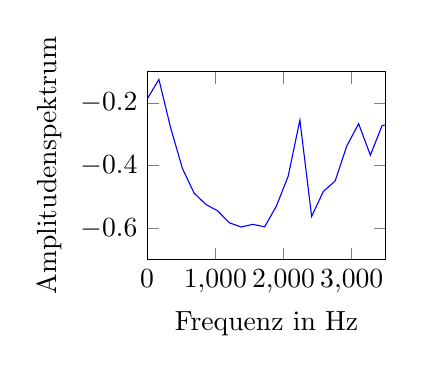
\begin{tikzpicture}

\begin{axis}[%
width=0.25\textwidth,
height=0.197\textwidth,
at={(0\textwidth,0\textwidth)},
scale only axis,
xmin=0,
xmax=3500,
xlabel={Frequenz in Hz},
ymin=-0.7,
ymax=-0.1,
ylabel={Amplitudenspektrum},
%title={$\text{Formanten f\"ur den Vokal \enquote}{\text{i}}$}
]
\addplot [color=blue,solid,forget plot]
  table[row sep=crcr]{%
0	-0.1870873676787\\
172.265625	-0.124606592043381\\
344.53125	-0.278971980502043\\
516.796875	-0.408552272077687\\
689.0625	-0.487382878228641\\
861.328125	-0.523481417803874\\
1033.59375	-0.543768039416707\\
1205.859375	-0.581938318802905\\
1378.125	-0.595244109407637\\
1550.390625	-0.586787106479387\\
1722.65625	-0.594810571612354\\
1894.921875	-0.52854416045969\\
2067.1875	-0.433815573300611\\
2239.453125	-0.254441702688233\\
2411.71875	-0.561540523033787\\
2583.984375	-0.481655266112142\\
2756.25	-0.448850362610164\\
2928.515625	-0.336331361460825\\
3100.78125	-0.265846718893173\\
3273.046875	-0.36601407031051\\
3445.3125	-0.27154698246101\\
3617.578125	-0.265874222160239\\
3789.84375	-0.505589755361803\\
3962.109375	-0.493064840245526\\
4134.375	-0.488697668563952\\
4306.640625	-0.50241665499048\\
4478.90625	-0.443373885568908\\
4651.171875	-0.376730549785729\\
4823.4375	-0.285470253800668\\
4995.703125	-0.251392727331721\\
5167.96875	-0.247911926741615\\
5340.234375	-0.224874455672336\\
5512.5	-0.157800464770028\\
5684.765625	-0.1800294293081\\
5857.03125	-0.247664864724133\\
6029.296875	-0.263915165617128\\
6201.5625	-0.176428925969494\\
6373.828125	-0.141180205091637\\
6546.09375	-0.387777081282331\\
6718.359375	-0.370707943332816\\
6890.625	-0.320616446386987\\
7062.890625	-0.243273513831002\\
7235.15625	-0.445014028915396\\
7407.421875	-0.503895570867559\\
7579.6875	-0.61510170950748\\
7751.953125	-0.560142047194254\\
7924.21875	-0.50446638188819\\
8096.484375	-0.621396958672453\\
8268.75	-0.689487013486006\\
8441.015625	-0.736726881637801\\
8613.28125	-0.625933838446098\\
8785.546875	-0.423570746609167\\
8957.8125	-0.457258481538982\\
9130.078125	-0.598761118950131\\
9302.34375	-0.50140752514791\\
9474.609375	-0.535967282788022\\
9646.875	-0.642958627677039\\
9819.140625	-0.4571264964318\\
9991.40625	-0.557372901488328\\
10163.671875	-0.690265690621624\\
10335.9375	-0.607809935105308\\
10508.203125	-0.739912404869531\\
10680.46875	-0.761826770053667\\
10852.734375	-0.597000622324391\\
11025	-0.469328678220118\\
11197.265625	-0.520478989918416\\
11369.53125	-0.518590660824286\\
11541.796875	-0.580155608736083\\
11714.0625	-0.646321232890602\\
11886.328125	-0.8012588907925\\
12058.59375	-0.700165049834895\\
12230.859375	-0.732953667034508\\
12403.125	-0.616466415278129\\
12575.390625	-0.560488197291204\\
12747.65625	-0.778365897312256\\
12919.921875	-0.755240265914003\\
13092.1875	-0.801364747751031\\
13264.453125	-0.857226371707966\\
13436.71875	-0.919279234333996\\
13608.984375	-0.946009484822061\\
13781.25	-0.893603138858667\\
13953.515625	-0.898704826963627\\
14125.78125	-0.913917797749607\\
14298.046875	-0.907415428936837\\
14470.3125	-0.850633074901554\\
14642.578125	-0.822242106711636\\
14814.84375	-0.912518836774858\\
14987.109375	-0.923232400919938\\
15159.375	-0.924110832271203\\
15331.640625	-0.923816100660652\\
15503.90625	-0.875929484987136\\
15676.171875	-0.862948400601403\\
15848.4375	-0.889977020534071\\
16020.703125	-0.921276581984284\\
16192.96875	-0.937071633237406\\
16365.234375	-0.930745205138123\\
16537.5	-0.951577204448038\\
16709.765625	-0.9371298296321\\
16882.03125	-0.918140206991247\\
17054.296875	-0.945910236340733\\
17226.5625	-0.923388271307007\\
17398.828125	-0.917916735778229\\
17571.09375	-0.959438227031189\\
17743.359375	-0.93134469589279\\
17915.625	-0.967436401730026\\
18087.890625	-0.940612412084777\\
18260.15625	-0.939514655053184\\
18432.421875	-0.934068294397959\\
18604.6875	-0.963882556330112\\
18776.953125	-0.958688859710452\\
18949.21875	-0.958339331785018\\
19121.484375	-0.955436833401938\\
19293.75	-0.96022875373091\\
19466.015625	-0.96897250385543\\
19638.28125	-0.979304288015029\\
19810.546875	-0.973442142568704\\
19982.8125	-0.966452999180048\\
20155.078125	-0.970027664140936\\
20327.34375	-0.992586844959336\\
20499.609375	-0.975733951179023\\
20671.875	-0.992750105749142\\
20844.140625	-1\\
21016.40625	-0.993068132208889\\
21188.671875	-0.989064179905442\\
21360.9375	-0.982378327232826\\
21533.203125	-0.991285556593491\\
21705.46875	-0.992114960027848\\
21877.734375	-0.982487871624791\\
};
\end{axis}
\end{tikzpicture}%
\end{scope}

\begin{scope}[scale = .3, xshift = \absheadposx+1500, yshift = 0]
\begin{axis}[%
width=0.8\columnwidth,
%height=0.5\columnwidth,
at={(0\textwidth,0\textwidth)},
scale only axis,
xmin=0,
xmax=3500,
xlabel={Frequenz f/Hz},
ymin=-60,
ymax=5,
ylabel={$|$I(f)$|$ in dB}
]
\addplot [color=blue,solid,forget plot]
  table[row sep=crcr]{%
-0.25	-94.4383425739265\\
0.25	-94.4425033029385\\
0.75	-94.4383425739265\\
1.25	-94.4258832392265\\
1.75	-94.4051934297753\\
2.25	-94.3763852935261\\
2.75	-94.3396129469626\\
3.25	-94.2950697172175\\
3.75	-94.2429847762108\\
4.25	-94.1836192859788\\
4.75	-94.1172621849195\\
5.25	-94.0442257484504\\
5.75	-93.9648410544102\\
6.25	-93.8794534747979\\
6.75	-93.7884183018958\\
7.25	-93.6920966003666\\
7.75	-93.5908513582826\\
8.25	-93.4850439911707\\
8.75	-93.3750312347523\\
9.25	-93.2611624449228\\
9.75	-93.1437773088547\\
10.25	-93.0232039583279\\
10.75	-92.8997574666384\\
11.25	-92.7737387028679\\
11.75	-92.6454335122139\\
12.25	-92.5151121880467\\
12.75	-92.383029200035\\
13.25	-92.2494231428284\\
13.75	-92.1145168710049\\
14.25	-91.9785177880281\\
14.75	-91.8416182595001\\
15.25	-91.7039961239045\\
15.75	-91.5658152770468\\
16.25	-91.4272263094388\\
16.75	-91.2883671787606\\
17.25	-91.149363902324\\
17.75	-91.0103312569967\\
18.25	-90.8713734762511\\
18.75	-90.7325849361451\\
19.25	-90.5940508237426\\
19.75	-90.4558477830128\\
20.25	-90.3180445346328\\
20.75	-90.1807024670676\\
21.25	-90.0438761974301\\
21.75	-89.9076141011551\\
22.25	-89.7719588102729\\
22.75	-89.6369476805002\\
23.25	-89.5026132277323\\
23.75	-89.3689835348366\\
24.25	-89.236082629833\\
24.75	-89.1039308367016\\
25.25	-88.9725451001778\\
25.75	-88.8419392859176\\
26.25	-88.7121244574723\\
26.75	-88.5831091314853\\
27.25	-88.4548995125337\\
27.75	-88.3274997089516\\
28.25	-88.2009119309903\\
28.75	-88.0751366725456\\
29.25	-87.9501728776719\\
29.75	-87.826018093033\\
30.25	-87.7026686073376\\
30.75	-87.5801195787369\\
31.25	-87.4583651512676\\
31.75	-87.3373985610097\\
32.25	-87.2172122329471\\
32.75	-87.0977978692089\\
33.25	-86.9791465294055\\
33.75	-86.8612487037339\\
34.25	-86.7440943794198\\
34.75	-86.6276731010733\\
35.25	-86.5119740254596\\
35.75	-86.3969859711528\\
36.25	-86.2826974635044\\
36.75	-86.1690967753398\\
37.25	-86.0561719637033\\
37.75	-85.9439109030417\\
38.25	-85.8323013150887\\
38.75	-85.7213307957508\\
39.25	-85.6109868392373\\
39.75	-85.5012568596967\\
40.25	-85.3921282105336\\
40.75	-85.2835882016459\\
41.25	-85.1756241147239\\
41.75	-85.0682232168045\\
42.25	-84.9613727722136\\
42.75	-84.8550600530451\\
43.25	-84.7492723482828\\
43.75	-84.6439969717126\\
44.25	-84.5392212686963\\
44.75	-84.4349326219075\\
45.25	-84.3311184561501\\
45.75	-84.2277662422873\\
46.25	-84.1248635003919\\
46.75	-84.0223978021664\\
47.25	-83.9203567726933\\
47.75	-83.8187280915774\\
48.25	-83.717499493522\\
48.75	-83.6166587683871\\
49.25	-83.5161937607651\\
49.75	-83.4160923691227\\
50.25	-83.3163425445216\\
50.75	-83.2169322889751\\
51.25	-83.1178496534351\\
51.75	-83.0190827354697\\
52.25	-82.920619676613\\
52.75	-82.8224486594444\\
53.25	-82.7245579043847\\
53.75	-82.6269356662448\\
54.25	-82.5295702305215\\
54.75	-82.4324499094735\\
55.25	-82.3355630379573\\
55.75	-82.2388979690648\\
56.25	-82.1424430695472\\
56.75	-82.0461867150292\\
57.25	-81.950117285034\\
57.75	-81.8542231578082\\
58.25	-81.7584927049476\\
58.75	-81.6629142858359\\
59.25	-81.5674762418872\\
59.75	-81.4721668905807\\
60.25	-81.3769745193171\\
60.75	-81.2818873790532\\
61.25	-81.1868936777362\\
61.75	-81.0919815735244\\
62.25	-80.9971391677985\\
62.75	-80.902354497899\\
63.25	-80.8076155297586\\
63.75	-80.7129101500472\\
64.25	-80.6182261583542\\
64.75	-80.5235512588802\\
65.25	-80.4288730519505\\
65.75	-80.334179025218\\
66.25	-80.2394565445534\\
66.75	-80.1446928446227\\
67.25	-80.0498750190965\\
67.75	-79.9549900105518\\
68.25	-79.8600245999462\\
68.75	-79.7649653957218\\
69.25	-79.6697988224825\\
69.75	-79.5745111092178\\
70.25	-79.4790882770721\\
70.75	-79.383516126602\\
71.25	-79.2877802245111\\
71.75	-79.191865889831\\
72.25	-79.0957581795031\\
72.75	-78.999441873338\\
73.25	-78.9029014583089\\
73.75	-78.8061211121334\\
74.25	-78.709084686115\\
74.75	-78.611775687176\\
75.25	-78.5141772590536\\
75.75	-78.4162721625904\\
76.25	-78.3180427550687\\
76.75	-78.2194709685259\\
77.25	-78.1205382869837\\
77.75	-78.0212257225254\\
78.25	-77.9215137901345\\
78.75	-77.8213824812288\\
79.25	-77.720811235786\\
79.75	-77.6197789129769\\
80.25	-77.5182637602049\\
80.75	-77.4162433804314\\
81.25	-77.3136946976841\\
81.75	-77.2105939206095\\
82.25	-77.1069165039293\\
82.75	-77.0026371076799\\
83.25	-76.8977295540246\\
83.75	-76.7921667815098\\
84.25	-76.6859207965557\\
84.75	-76.5789626219783\\
85.25	-76.4712622423214\\
85.75	-76.3627885457602\\
86.25	-76.2535092623116\\
86.75	-76.1433908980601\\
87.25	-76.0323986651014\\
87.75	-75.920496406847\\
88.25	-75.8076465183313\\
88.75	-75.6938098611108\\
89.25	-75.5789456723072\\
89.75	-75.4630114673185\\
90.25	-75.3459629356511\\
90.75	-75.2277538292971\\
91.25	-75.1083358430059\\
91.75	-74.9876584857428\\
92.25	-74.8656689425512\\
92.75	-74.7423119259545\\
93.25	-74.6175295159414\\
93.75	-74.4912609874767\\
94.25	-74.3634426243697\\
94.75	-74.2340075181882\\
95.25	-74.1028853507837\\
95.75	-73.9700021588003\\
96.25	-73.8352800783815\\
96.75	-73.6986370680505\\
97.25	-73.5599866075268\\
97.75	-73.4192373699409\\
98.25	-73.2762928646181\\
98.75	-73.1310510472349\\
99.25	-72.9834038937425\\
99.75	-72.8332369339895\\
100.25	-72.6804287404262\\
100.75	-72.5248503666597\\
101.25	-72.3663647298944\\
101.75	-72.2048259304744\\
102.25	-72.0400785007565\\
102.75	-71.8719565744193\\
103.25	-71.7002829659861\\
103.75	-71.5248681487909\\
104.25	-71.3455091177964\\
104.75	-71.1619881215086\\
105.25	-70.9740712447131\\
105.75	-70.7815068207288\\
106.25	-70.5840236482888\\
106.75	-70.3813289838869\\
107.25	-70.1731062752927\\
107.75	-69.9590125957895\\
108.25	-69.7386757312682\\
108.75	-69.5116908633485\\
109.25	-69.2776167808313\\
109.75	-69.0359715385841\\
110.25	-68.7862274668773\\
110.75	-68.5278054145597\\
111.25	-68.2600680854942\\
111.75	-67.9823122983993\\
112.25	-67.6937599645656\\
112.75	-67.3935475346444\\
113.25	-67.0807136136858\\
113.75	-66.7541843820672\\
114.25	-66.4127563892415\\
114.75	-66.0550762102468\\
115.25	-65.6796163801776\\
115.75	-65.2846469696401\\
116.25	-64.8682021794001\\
116.75	-64.4280415107801\\
117.25	-63.9616056130547\\
117.75	-63.4659682540297\\
118.25	-62.9377889483646\\
118.75	-62.3732777174692\\
119.25	-61.7681991302678\\
119.75	-61.1179790564134\\
120.25	-60.4180650502653\\
120.75	-59.6649149020051\\
121.25	-58.8586065807823\\
121.75	-58.0099686951319\\
122.25	-57.1619518017708\\
122.75	-56.4654790009217\\
123.25	-56.5496587111119\\
123.75	-62.9143249259129\\
124.25	-43.3688731539547\\
124.75	-11.9900222001443\\
125.25	-6.78271294059886\\
125.75	-16.5578137201217\\
126.25	-51.3248574230745\\
126.75	-59.8628531891147\\
127.25	-56.9325964375803\\
127.75	-57.2273390533597\\
128.25	-58.0518960326566\\
128.75	-58.9762518635147\\
129.25	-59.8881698175795\\
129.75	-60.7547363864306\\
130.25	-61.5678592073149\\
130.75	-62.327983440334\\
131.25	-63.0384524311005\\
131.75	-63.7033907905205\\
132.25	-64.3268892240077\\
132.75	-64.9127052836891\\
133.25	-65.4641762125291\\
133.75	-65.9842189607838\\
134.25	-66.4753639789448\\
134.75	-66.9397995958508\\
135.25	-67.379417046435\\
135.75	-67.7958521642178\\
136.25	-68.1905224362096\\
136.75	-68.5646593004219\\
137.25	-68.9193360509473\\
137.75	-69.2554918765388\\
138.25	-69.5739525731561\\
138.75	-69.8754484239236\\
139.25	-70.1606296717466\\
139.75	-70.4300799392207\\
140.25	-70.6843278856686\\
140.75	-70.9238573352597\\
141.25	-71.1491160638588\\
141.75	-71.3605233951092\\
142.25	-71.5584767273257\\
142.75	-71.7433570910305\\
143.25	-71.9155338212601\\
143.75	-72.0753684180715\\
144.25	-72.2232176619214\\
144.75	-72.3594360468542\\
145.25	-72.4843775928184\\
145.75	-72.5983970981648\\
146.25	-72.7018508937457\\
146.75	-72.7950971605043\\
147.25	-72.8784958725253\\
147.75	-72.9524084269169\\
148.25	-73.0171970204034\\
148.75	-73.0732238300317\\
149.25	-73.1208500519879\\
149.75	-73.1604348482162\\
150.25	-73.1923342455695\\
150.75	-73.2169000267216\\
151.25	-73.2344786463015\\
151.75	-73.2454101998466\\
152.25	-73.2500274674391\\
152.75	-73.2486550484229\\
153.25	-73.2416085985689\\
153.75	-73.2291941765185\\
154.25	-73.2117077024088\\
154.75	-73.1894345282242\\
155.25	-73.1626491166986\\
155.75	-73.131614823433\\
156.25	-73.0965837752905\\
156.75	-73.0577968369981\\
157.25	-73.0154836571928\\
157.75	-72.9698627848135\\
158.25	-72.9211418466983\\
158.75	-72.8695177774547\\
159.25	-72.8151770930464\\
159.75	-72.7582962000632\\
160.25	-72.6990417332482\\
160.75	-72.6375709145107\\
161.25	-72.5740319273553\\
161.75	-72.5085643013298\\
162.25	-72.4412993017783\\
162.75	-72.3723603208223\\
163.25	-72.3018632660958\\
163.75	-72.2299169443132\\
164.25	-72.1566234372612\\
164.75	-72.0820784682566\\
165.25	-72.0063717575235\\
165.75	-71.9295873652963\\
166.25	-71.8518040217715\\
166.75	-71.7730954433004\\
167.25	-71.6935306344427\\
167.75	-71.6131741757018\\
168.25	-71.5320864969167\\
168.75	-71.4503241364316\\
169.25	-71.3679399862617\\
169.75	-71.284983523572\\
170.25	-71.2015010288457\\
170.75	-71.117535791178\\
171.25	-71.0331283011613\\
171.75	-70.9483164318636\\
172.25	-70.8631356084101\\
172.75	-70.7776189666889\\
173.25	-70.6917975017043\\
173.75	-70.6057002060956\\
174.25	-70.5193541993285\\
174.75	-70.4327848480592\\
175.25	-70.3460158781502\\
175.75	-70.2590694788043\\
176.25	-70.1719663992643\\
176.75	-70.0847260385037\\
177.25	-69.9973665283191\\
177.75	-69.9099048102078\\
178.25	-69.8223567064011\\
178.75	-69.7347369854016\\
179.25	-69.647059422348\\
179.75	-69.559336854524\\
180.25	-69.4715812322941\\
180.75	-69.383803665748\\
181.25	-69.2960144673042\\
181.75	-69.2082231905159\\
182.25	-69.1204386653065\\
182.75	-69.032669029842\\
183.25	-68.9449217592407\\
183.75	-68.8572036913045\\
184.25	-68.7695210494422\\
184.75	-68.6818794629493\\
185.25	-68.5942839847919\\
185.75	-68.5067391070367\\
186.25	-68.4192487740584\\
186.75	-68.3318163936449\\
187.25	-68.2444448461206\\
187.75	-68.1571364915717\\
188.25	-68.0698931753431\\
188.75	-67.9827162317526\\
189.25	-67.8956064863121\\
189.75	-67.8085642563489\\
190.25	-67.7215893502149\\
190.75	-67.6346810651116\\
191.25	-67.5478381836024\\
191.75	-67.4610589688753\\
192.25	-67.3743411588022\\
192.75	-67.2876819588621\\
193.25	-67.2010780339562\\
193.75	-67.1145254991713\\
194.25	-67.0280199095262\\
194.75	-66.9415562487325\\
195.25	-66.8551289170081\\
195.75	-66.7687317179645\\
196.25	-66.682357844594\\
196.75	-66.5959998643772\\
197.25	-66.5096497035251\\
197.75	-66.4232986303677\\
198.25	-66.3369372378974\\
198.75	-66.250555425469\\
199.25	-66.1641423796583\\
199.75	-66.0776865542674\\
200.25	-65.991175649474\\
200.75	-65.9045965901012\\
201.25	-65.8179355029921\\
201.75	-65.7311776934584\\
202.25	-65.6443076207731\\
202.75	-65.5573088726651\\
203.25	-65.4701641387708\\
203.75	-65.3828551829898\\
204.25	-65.2953628146804\\
204.75	-65.207666858629\\
205.25	-65.1197461237121\\
205.75	-65.0315783701629\\
206.25	-64.9431402753453\\
206.75	-64.8544073979258\\
207.25	-64.7653541403191\\
207.75	-64.6759537092791\\
208.25	-64.5861780744808\\
208.75	-64.4959979249361\\
209.25	-64.4053826230606\\
209.75	-64.3143001561978\\
210.25	-64.2227170853838\\
210.75	-64.1305984911177\\
211.25	-64.037907915878\\
211.75	-63.9446073031037\\
212.25	-63.8506569323287\\
212.75	-63.7560153501303\\
213.25	-63.6606392965219\\
213.75	-63.5644836263802\\
214.25	-63.4675012254622\\
214.75	-63.3696429205212\\
215.25	-63.2708573829851\\
215.75	-63.1710910256055\\
216.25	-63.0702878914278\\
216.75	-62.9683895343677\\
217.25	-62.8653348906051\\
217.75	-62.7610601399243\\
218.25	-62.6554985560407\\
218.75	-62.5485803448476\\
219.25	-62.4402324694049\\
219.75	-62.3303784603587\\
220.25	-62.2189382103391\\
220.75	-62.1058277507104\\
221.25	-61.9909590088704\\
221.75	-61.8742395440733\\
222.25	-61.7555722595163\\
222.75	-61.6348550881505\\
223.25	-61.5119806493632\\
223.75	-61.3868358733199\\
224.25	-61.2593015893407\\
224.75	-61.129252074209\\
225.25	-60.9965545557689\\
225.75	-60.8610686665309\\
226.25	-60.7226458412766\\
226.75	-60.5811286518059\\
227.25	-60.4363500709778\\
227.75	-60.2881326570485\\
228.25	-60.1362876479582\\
228.75	-59.9806139536372\\
229.25	-59.8208970325397\\
229.75	-59.6569076364156\\
230.25	-59.4884004047298\\
230.75	-59.3151122870506\\
231.25	-59.1367607680495\\
231.75	-58.95304186536\\
232.25	-58.7636278652755\\
232.75	-58.5681647549347\\
233.25	-58.3662693020006\\
233.75	-58.157525723603\\
234.25	-57.9414818750984\\
234.75	-57.7176448755676\\
235.25	-57.485476070338\\
235.75	-57.2443852105122\\
236.25	-56.9937237046581\\
236.75	-56.7327767674726\\
237.25	-56.4607542532322\\
237.75	-56.1767799169441\\
238.25	-55.8798787921287\\
238.75	-55.5689623103452\\
239.25	-55.2428107143598\\
239.75	-54.9000522374883\\
240.25	-54.5391384454906\\
240.75	-54.1583150866394\\
241.25	-53.755587819198\\
241.75	-53.3286823883245\\
242.25	-52.8749994292804\\
242.75	-52.391565558509\\
243.25	-51.8749858220419\\
243.75	-51.321410246101\\
244.25	-50.7265446489849\\
244.75	-50.08577642914\\
245.25	-49.3945846312073\\
245.75	-48.6496582358787\\
246.25	-47.8518608448083\\
246.75	-47.0144209094212\\
247.25	-46.1879584780304\\
247.75	-45.5523144118615\\
248.25	-45.8964380141639\\
248.75	-56.828617095311\\
249.25	-28.7024518956255\\
249.75	-4.70792109373025\\
250.25	-1.60325981275531\\
250.75	-13.9790407008642\\
251.25	-45.2822389364891\\
251.75	-48.3405592230755\\
252.25	-46.3384873877839\\
252.75	-46.7734649651522\\
253.25	-47.6447639486622\\
253.75	-48.5957810285641\\
254.25	-49.5304537574016\\
254.75	-50.4205841736613\\
255.25	-51.259671369388\\
255.75	-52.0487538807132\\
256.25	-52.7914266359981\\
256.75	-53.4919516387272\\
257.25	-54.154527050811\\
257.75	-54.78301959325\\
258.25	-55.380888501059\\
258.75	-55.9511883380299\\
259.25	-56.4966021885573\\
259.75	-57.0194840741314\\
260.25	-57.5219015140131\\
260.75	-58.0056745978901\\
261.25	-58.4724104057403\\
261.75	-58.9235327025507\\
262.25	-59.3603072857651\\
262.75	-59.7838635145045\\
263.25	-60.1952125651478\\
263.75	-60.5952629160888\\
264.25	-60.9848335026989\\
264.75	-61.3646649189523\\
265.25	-61.7354289822635\\
265.75	-62.0977369255292\\
266.25	-62.4521464356399\\
266.75	-62.7991677202647\\
267.25	-63.139268753682\\
267.75	-63.4728798268173\\
268.25	-63.8003975055874\\
268.75	-64.1221880843239\\
269.25	-64.438590606789\\
269.75	-64.7499195155468\\
270.25	-65.0564669807387\\
270.75	-65.3585049512709\\
271.25	-65.6562869647375\\
271.75	-65.9500497468336\\
272.25	-66.2400146263533\\
272.75	-66.5263887879564\\
273.25	-66.809366381595\\
273.75	-67.0891295047026\\
274.25	-67.3658490708784\\
274.75	-67.6396855767862\\
275.25	-67.9107897772548\\
275.75	-68.1793032770645\\
276.25	-68.4453590466413\\
276.75	-68.7090818677265\\
277.25	-68.9705887141325\\
277.75	-69.229989071817\\
278.25	-69.4873852017508\\
278.75	-69.742872348372\\
279.25	-69.9965388958082\\
279.75	-70.2484664735106\\
280.25	-70.4987300124399\\
280.75	-70.747397752519\\
281.25	-70.9945312016506\\
281.75	-71.2401850462627\\
282.25	-71.4844070130218\\
282.75	-71.7272376810991\\
283.25	-71.9687102441546\\
283.75	-72.2088502210529\\
284.25	-72.4476751142267\\
284.75	-72.6851940145944\\
285.25	-72.9214071520142\\
285.75	-73.1563053904459\\
286.25	-73.3898696673102\\
286.75	-73.6220703770176\\
287.25	-73.8528666993026\\
287.75	-74.0822058738813\\
288.25	-74.3100224241096\\
288.75	-74.5362373337459\\
289.25	-74.7607571827191\\
289.75	-74.9834732499641\\
290.25	-75.2042605939782\\
290.75	-75.4229771247924\\
291.25	-75.6394626845712\\
291.75	-75.8535381580601\\
292.25	-76.0650046385432\\
292.75	-76.273642679847\\
293.25	-76.4792116700634\\
293.75	-76.6814493679667\\
294.25	-76.8800716482646\\
294.75	-77.0747725066391\\
295.25	-77.2652243794297\\
295.75	-77.4510788355387\\
296.25	-77.6319676988497\\
296.75	-77.8075046577428\\
297.25	-77.9772874133488\\
297.75	-78.1409004094275\\
298.25	-78.297918173672\\
298.75	-78.4479092824171\\
299.25	-78.5904409381747\\
299.75	-78.7250841224657\\
300.25	-78.8514192558939\\
300.75	-78.9690422646818\\
301.25	-79.0775709199628\\
301.75	-79.176651285295\\
302.25	-79.2659640818832\\
302.75	-79.3452307628125\\
303.25	-79.414219079307\\
303.75	-79.4727479262412\\
304.25	-79.5206912712405\\
304.75	-79.5579810020382\\
305.25	-79.5846085687295\\
305.75	-79.600625348576\\
306.25	-79.6061417175111\\
306.75	-79.6013248701404\\
307.25	-79.5863954845855\\
307.75	-79.561623375818\\
308.25	-79.5273223181234\\
308.75	-79.4838442417903\\
309.25	-79.4315730203626\\
309.75	-79.3709180631399\\
310.25	-79.3023079146342\\
310.75	-79.2261840405934\\
311.25	-79.1429949517295\\
311.75	-79.0531907841903\\
312.25	-78.9572184226933\\
312.75	-78.8555172203075\\
313.25	-78.7485153398883\\
313.75	-78.6366267169595\\
314.25	-78.5202486236725\\
314.75	-78.3997597975477\\
315.25	-78.2755190878222\\
315.75	-78.147864565194\\
316.25	-78.0171130373766\\
316.75	-77.8835599123586\\
317.25	-77.7474793529642\\
317.75	-77.6091246696463\\
318.25	-77.4687289028159\\
318.75	-77.3265055510599\\
319.25	-77.1826494068519\\
319.75	-77.0373374666516\\
320.25	-76.8907298873281\\
320.75	-76.74297096555\\
321.25	-76.5941901210761\\
321.75	-76.4445028686669\\
322.25	-76.2940117666909\\
322.75	-76.1428073333516\\
323.25	-75.990968923891\\
323.75	-75.8385655641528\\
324.25	-75.6856567375775\\
324.75	-75.5322931239923\\
325.25	-75.3785172897358\\
325.75	-75.2243643293921\\
326.25	-75.0698624601322\\
326.75	-74.9150335701051\\
327.25	-74.7598937226582\\
327.75	-74.6044536184281\\
328.25	-74.4487190174419\\
328.75	-74.2926911234765\\
329.25	-74.1363669329126\\
329.75	-73.9797395503006\\
330.25	-73.8227984727957\\
330.75	-73.6655298455218\\
331.25	-73.5079166898372\\
331.75	-73.3499391063455\\
332.25	-73.1915744543799\\
332.75	-73.0327975095694\\
333.25	-72.8735806009516\\
333.75	-72.7138937289889\\
334.25	-72.5537046657102\\
334.75	-72.392979038078\\
335.25	-72.2316803955695\\
335.75	-72.0697702628404\\
336.25	-71.9072081782288\\
336.75	-71.7439517187567\\
337.25	-71.5799565121723\\
337.75	-71.4151762364853\\
338.25	-71.249562607344\\
338.75	-71.0830653535059\\
339.25	-70.9156321805614\\
339.75	-70.7472087229738\\
340.25	-70.5777384843996\\
340.75	-70.4071627661655\\
341.25	-70.2354205836693\\
341.75	-70.062448570375\\
342.25	-69.8881808689682\\
342.75	-69.7125490091162\\
343.25	-69.535481771169\\
343.75	-69.3569050349972\\
344.25	-69.1767416130352\\
344.75	-68.9949110664341\\
345.25	-68.8113295030725\\
345.75	-68.6259093559822\\
346.25	-68.4385591405438\\
346.75	-68.2491831885764\\
347.25	-68.0576813571908\\
347.75	-67.8639487099803\\
348.25	-67.6678751678019\\
348.75	-67.4693451260189\\
349.25	-67.2682370346561\\
349.75	-67.0644229374284\\
350.25	-66.8577679650414\\
350.75	-66.6481297775217\\
351.25	-66.4353579495881\\
351.75	-66.2192932922085\\
352.25	-65.9997671024876\\
352.75	-65.7766003328624\\
353.25	-65.54960266921\\
353.75	-65.3185715058784\\
354.25	-65.0832908037582\\
354.75	-64.8435298153008\\
355.25	-64.5990416577518\\
355.75	-64.349561712756\\
356.25	-64.0948058267734\\
356.75	-63.8344682823152\\
357.25	-63.5682195046981\\
357.75	-63.2957034626362\\
358.25	-63.0165347133017\\
358.75	-62.7302950331965\\
359.25	-62.4365295649184\\
359.75	-62.1347423962338\\
360.25	-61.824391471229\\
360.75	-61.5048827130434\\
361.25	-61.175563212983\\
361.75	-60.8357133107493\\
362.25	-60.4845373540567\\
362.75	-60.1211528819991\\
363.25	-59.7445779243071\\
363.75	-59.3537160479052\\
364.25	-58.9473387143497\\
364.75	-58.5240644417735\\
365.25	-58.0823342053557\\
365.75	-57.6203824890355\\
366.25	-57.1362034780282\\
366.75	-56.627512182609\\
367.25	-56.0917010737548\\
367.75	-55.5257946558795\\
368.25	-54.9264085332471\\
368.75	-54.289728715573\\
369.25	-53.6115476431534\\
369.75	-52.8874416800642\\
370.25	-52.1132926047389\\
370.75	-51.2866622965009\\
371.25	-50.4104011829712\\
371.75	-49.5026593408774\\
372.25	-48.6280259927394\\
372.75	-48.0162572676959\\
373.25	-48.7418178920483\\
373.75	-71.5508017105879\\
374.25	-26.4854953440571\\
374.75	-7.30352868019295\\
375.25	-6.23079727509385\\
375.75	-21.6081654119154\\
376.25	-54.6326273600718\\
376.75	-48.9919455364187\\
377.25	-47.7819229797393\\
377.75	-48.2928589502265\\
378.25	-49.1279551122924\\
378.75	-50.0108623034038\\
379.25	-50.8657882423304\\
379.75	-51.6712995465898\\
380.25	-52.4235407607879\\
380.75	-53.1246914977364\\
381.25	-53.7788684556959\\
381.75	-54.3905781493179\\
382.25	-54.9641314970626\\
382.75	-55.5034427347355\\
383.25	-56.0119854851453\\
383.75	-56.4928117342359\\
384.25	-56.9485934047576\\
384.75	-57.3816692060564\\
385.25	-57.7940895596537\\
385.75	-58.1876569269737\\
386.25	-58.5639608787489\\
386.75	-58.9244081059633\\
387.25	-59.2702479001623\\
387.75	-59.6025937160642\\
388.25	-59.9224414084558\\
388.75	-60.2306846730887\\
389.25	-60.5281281478242\\
389.75	-60.8154985589896\\
390.25	-61.0934542341266\\
390.75	-61.3625932475211\\
391.25	-61.6234604188917\\
391.75	-61.8765533474566\\
392.25	-62.122327632173\\
392.75	-62.36120140316\\
393.25	-62.5935592681815\\
393.75	-62.8197557607379\\
394.25	-63.0401183620948\\
394.75	-63.2549501578809\\
395.25	-63.4645321802427\\
395.75	-63.6691254785745\\
396.25	-63.8689729552331\\
396.75	-64.0643009971528\\
397.25	-64.2553209296917\\
397.75	-64.4422303152072\\
398.25	-64.6252141156392\\
398.75	-64.8044457356717\\
399.25	-64.9800879607502\\
399.75	-65.1522938023032\\
400.25	-65.3212072608621\\
400.75	-65.4869640163736\\
401.25	-65.6496920538041\\
401.75	-65.8095122311029\\
402.25	-65.9665387957163\\
402.75	-66.1208798550792\\
403.25	-66.2726378058607\\
403.75	-66.4219097261693\\
404.25	-66.5687877344312\\
404.75	-66.7133593182325\\
405.25	-66.8557076360331\\
405.75	-66.9959117943455\\
406.25	-67.1340471026769\\
406.75	-67.2701853082897\\
407.25	-67.4043948126105\\
407.75	-67.5367408709275\\
408.25	-67.6672857768431\\
408.75	-67.7960890327962\\
409.25	-67.9232075078392\\
409.75	-68.0486955837298\\
410.25	-68.1726052902966\\
410.75	-68.2949864309396\\
411.25	-68.4158866990458\\
411.75	-68.5353517860216\\
412.25	-68.6534254815802\\
412.75	-68.7701497668554\\
413.25	-68.8855649008667\\
413.75	-68.9997095008055\\
414.25	-69.1126206165683\\
414.75	-69.2243337999287\\
415.25	-69.3348831686941\\
415.75	-69.4443014661698\\
416.25	-69.5526201162149\\
416.75	-69.6598692741542\\
417.25	-69.7660778737798\\
417.75	-69.8712736706554\\
418.25	-69.9754832819163\\
418.75	-70.078732222737\\
419.25	-70.1810449396215\\
419.75	-70.2824448406513\\
420.25	-70.3829543228225\\
420.75	-70.4825947965668\\
421.25	-70.5813867075644\\
421.75	-70.6793495559239\\
422.25	-70.7765019128017\\
422.75	-70.87286143452\\
423.25	-70.9684448742341\\
423.75	-71.0632680911849\\
424.25	-71.1573460575688\\
424.75	-71.2506928630437\\
425.25	-71.3433217168822\\
425.75	-71.4352449477779\\
426.25	-71.5264740012964\\
426.75	-71.6170194349594\\
427.25	-71.7068909109445\\
427.75	-71.7960971863676\\
428.25	-71.8846461011198\\
428.75	-71.9725445632136\\
429.25	-72.0597985315908\\
429.75	-72.1464129963424\\
430.25	-72.2323919562758\\
430.75	-72.3177383937689\\
431.25	-72.4024542468388\\
431.75	-72.4865403783515\\
432.25	-72.5699965422937\\
432.75	-72.6528213470256\\
433.25	-72.7350122154305\\
433.75	-72.8165653418717\\
434.25	-72.8974756458758\\
434.75	-72.977736722448\\
435.25	-73.0573407889372\\
435.75	-73.1362786283733\\
436.25	-73.214539529188\\
436.75	-73.2921112212555\\
437.25	-73.368979808187\\
437.75	-73.4451296958472\\
438.25	-73.5205435169837\\
438.75	-73.595202052089\\
439.25	-73.6690841463242\\
439.75	-73.7421666226685\\
440.25	-73.8144241912755\\
440.75	-73.8858293551502\\
441.25	-73.9563523122647\\
441.75	-74.0259608542948\\
442.25	-74.0946202621923\\
442.75	-74.1622931988807\\
443.25	-74.2289395994218\\
443.75	-74.2945165590711\\
444.25	-74.35897821973\\
444.75	-74.4222756553807\\
445.25	-74.4843567572004\\
445.75	-74.5451661191504\\
446.25	-74.6046449249523\\
446.75	-74.6627308374951\\
447.25	-74.7193578918366\\
447.75	-74.774456393112\\
448.25	-74.8279528208033\\
448.75	-74.8797697409683\\
449.25	-74.9298257281761\\
449.75	-74.9780352990594\\
450.25	-75.0243088595127\\
450.75	-75.0685526677192\\
451.25	-75.1106688153077\\
451.75	-75.1505552290398\\
452.25	-75.1881056954993\\
452.75	-75.2232099113223\\
453.25	-75.2557535614901\\
453.75	-75.2856184281847\\
454.25	-75.3126825326002\\
454.75	-75.3368203119609\\
455.25	-75.3579028337532\\
455.75	-75.3757980488879\\
456.25	-75.3903710851207\\
456.75	-75.4014845815708\\
457.25	-75.4089990646406\\
457.75	-75.4127733649554\\
458.25	-75.412665074232\\
458.75	-75.4085310401506\\
459.25	-75.4002278964311\\
459.75	-75.3876126243768\\
460.25	-75.3705431411836\\
460.75	-75.3488789093349\\
461.25	-75.3224815604556\\
461.75	-75.2912155260787\\
462.25	-75.2549486669707\\
462.75	-75.2135528919428\\
463.25	-75.1669047565166\\
463.75	-75.114886031438\\
464.25	-75.0573842308468\\
464.75	-74.9942930899659\\
465.25	-74.9255129824546\\
465.75	-74.8509512680983\\
466.25	-74.7705225622774\\
466.75	-74.6841489196411\\
467.25	-74.5917599255947\\
467.75	-74.4932926905599\\
468.25	-74.3886917434263\\
468.75	-74.2779088221542\\
469.25	-74.1609025610395\\
469.75	-74.0376380756676\\
470.25	-73.9080864480147\\
470.75	-73.77222411543\\
471.25	-73.6300321683409\\
471.75	-73.4814955623924\\
472.25	-73.3266022513322\\
472.75	-73.1653422473303\\
473.25	-72.9977066154367\\
473.75	-72.8236864086712\\
474.25	-72.6432715496919\\
474.75	-72.4564496642181\\
475.25	-72.263204870292\\
475.75	-72.0635165261837\\
476.25	-71.8573579381978\\
476.75	-71.6446950279144\\
477.25	-71.4254849564392\\
477.75	-71.1996747011159\\
478.25	-70.9671995778106\\
478.75	-70.7279816993329\\
479.25	-70.4819283577708\\
479.75	-70.2289303154424\\
480.25	-69.9688599857729\\
480.75	-69.7015694815701\\
481.25	-69.426888503843\\
481.75	-69.1446220393239\\
482.25	-68.8545478290698\\
482.75	-68.5564135637328\\
483.25	-68.2499337530537\\
483.75	-67.9347862075433\\
484.25	-67.6106080588015\\
484.75	-67.2769912310241\\
485.25	-66.9334772594055\\
485.75	-66.5795513306962\\
486.25	-66.2146353963242\\
486.75	-65.838080178333\\
487.25	-65.4491558519498\\
487.75	-65.0470411449418\\
488.25	-64.6308105423971\\
488.75	-64.1994192263917\\
489.25	-63.7516853153343\\
489.75	-63.2862689039939\\
490.25	-62.801647357412\\
490.75	-62.2960863130442\\
491.25	-61.7676059651717\\
491.75	-61.2139425891681\\
492.25	-60.6325062155495\\
492.75	-60.0203375343397\\
493.25	-59.3740719167369\\
493.75	-58.6899290815232\\
494.25	-57.9637709358969\\
494.75	-57.1913261680641\\
495.25	-56.3688177990566\\
495.75	-55.4945917990107\\
496.25	-54.573387973492\\
496.75	-53.6283019092966\\
497.25	-52.7387965448757\\
497.75	-52.1918427729062\\
498.25	-53.4398779610317\\
498.75	-57.9797554383091\\
499.25	-25.8014621644716\\
499.75	-10.257832348695\\
500.25	-11.2004747246728\\
500.75	-30.1860753718157\\
501.25	-76.7764976502099\\
501.75	-52.1473958245962\\
502.25	-51.4411349384824\\
502.75	-52.0136540176984\\
503.25	-52.8328877572577\\
503.75	-53.6781518629163\\
504.25	-54.4881238735288\\
504.75	-55.2461591895401\\
505.25	-55.9502107713451\\
505.75	-56.6031893773357\\
506.25	-57.2095112560848\\
506.75	-57.7737979001557\\
507.25	-58.3003934838252\\
507.75	-58.7932092285477\\
508.25	-59.2557003662053\\
508.75	-59.6908949158975\\
509.25	-60.1014398443262\\
509.75	-60.489649985283\\
510.25	-60.8575538037311\\
510.75	-61.206933961857\\
511.25	-61.5393623424219\\
511.75	-61.8562298888049\\
512.25	-62.1587718699058\\
512.75	-62.4480892224109\\
513.25	-62.725166580854\\
513.75	-62.9908875327107\\
514.25	-63.2460475567442\\
514.75	-63.4913650288292\\
515.25	-63.7274906144904\\
515.75	-63.9550153121807\\
516.25	-64.1744773652844\\
516.75	-64.3863682228339\\
517.25	-64.5911376977422\\
517.75	-64.7891984458256\\
518.25	-64.9809298680014\\
518.75	-65.1666815209452\\
519.25	-65.3467761074642\\
519.75	-65.5215121063186\\
520.25	-65.6911660917219\\
520.75	-65.8559947849044\\
521.25	-66.0162368736159\\
521.75	-66.1721146300347\\
522.25	-66.3238353530434\\
522.75	-66.4715926570447\\
523.25	-66.6155676263435\\
523.75	-66.755929851427\\
524.25	-66.8928383612456\\
524.75	-67.0264424636757\\
525.25	-67.1568825047269\\
525.75	-67.2842905556774\\
526.25	-67.4087910361354\\
526.75	-67.5305012800205\\
527.25	-67.649532050582\\
527.75	-67.7659880098296\\
528.25	-67.8799681471008\\
528.75	-67.9915661709328\\
529.25	-68.1008708679199\\
529.75	-68.207966431815\\
530.25	-68.3129327657688\\
530.75	-68.4158457602723\\
531.25	-68.5167775490941\\
531.75	-68.6157967452537\\
532.25	-68.7129686588519\\
532.75	-68.8083554983953\\
533.25	-68.902016557076\\
533.75	-68.9940083853227\\
534.25	-69.0843849508069\\
534.75	-69.1731977869679\\
535.25	-69.2604961310213\\
535.75	-69.3463270523148\\
536.25	-69.4307355718213\\
536.75	-69.5137647734805\\
537.25	-69.595455908034\\
537.75	-69.6758484899392\\
538.25	-69.7549803878994\\
538.75	-69.8328879094921\\
539.25	-69.9096058803409\\
539.75	-69.9851677182311\\
540.25	-70.0596055025435\\
540.75	-70.1329500393397\\
541.25	-70.2052309224077\\
541.75	-70.2764765905545\\
542.25	-70.3467143814002\\
542.75	-70.4159705819156\\
543.25	-70.4842704759194\\
543.75	-70.5516383887379\\
544.25	-70.6180977292111\\
544.75	-70.6836710292127\\
545.25	-70.7483799808493\\
545.75	-70.8122454714708\\
546.25	-70.8752876166351\\
546.75	-70.9375257911448\\
547.25	-70.9989786582712\\
547.75	-71.0596641972673\\
548.25	-71.1195997292701\\
548.75	-71.1788019416768\\
549.25	-71.2372869110791\\
549.75	-71.295070124832\\
550.25	-71.352166501321\\
550.75	-71.4085904090016\\
551.25	-71.4643556842596\\
551.75	-71.5194756481532\\
552.25	-71.5739631220804\\
552.75	-71.6278304424269\\
553.25	-71.6810894742223\\
553.75	-71.7337516238532\\
554.25	-71.7858278508624\\
554.75	-71.8373286788651\\
555.25	-71.8882642056092\\
555.75	-71.9386441122059\\
556.25	-71.9884776715497\\
556.75	-72.0377737559475\\
557.25	-72.0865408439715\\
557.75	-72.13478702655\\
558.25	-72.1825200123068\\
558.75	-72.229747132154\\
559.25	-72.276475343147\\
559.75	-72.3227112316033\\
560.25	-72.368461015482\\
560.75	-72.4137305460292\\
561.25	-72.4585253086743\\
561.75	-72.50285042318\\
562.25	-72.5467106430213\\
562.75	-72.5901103540118\\
563.25	-72.633053572099\\
563.75	-72.6755439404051\\
564.25	-72.7175847253892\\
564.75	-72.7591788121827\\
565.25	-72.8003286990329\\
565.75	-72.8410364908353\\
566.25	-72.8813038917165\\
566.75	-72.9211321966347\\
567.25	-72.960522281948\\
567.75	-72.9994745949108\\
568.25	-73.0379891420475\\
568.75	-73.0760654763439\\
569.25	-73.113702683202\\
569.75	-73.1508993650912\\
570.25	-73.1876536248241\\
570.75	-73.2239630473848\\
571.25	-73.2598246802239\\
571.75	-73.2952350119342\\
572.25	-73.330189949209\\
572.75	-73.3646847919843\\
573.25	-73.3987142066475\\
573.75	-73.4322721972014\\
574.25	-73.4653520742498\\
574.75	-73.4979464216636\\
575.25	-73.5300470607931\\
575.75	-73.5616450120509\\
576.25	-73.5927304537067\\
576.75	-73.6232926777078\\
577.25	-73.6533200423266\\
577.75	-73.6827999214324\\
578.25	-73.7117186501563\\
578.75	-73.7400614667139\\
579.25	-73.7678124501259\\
579.75	-73.7949544535681\\
580.25	-73.8214690330502\\
580.75	-73.8473363711203\\
581.25	-73.8725351952559\\
581.75	-73.8970426905928\\
582.25	-73.9208344066121\\
582.75	-73.9438841573867\\
583.25	-73.9661639149656\\
583.75	-73.9876436954427\\
584.25	-74.0082914372415\\
584.75	-74.0280728711063\\
585.25	-74.0469513812788\\
585.75	-74.0648878572987\\
586.25	-74.0818405358509\\
586.75	-74.097764832042\\
587.25	-74.1126131594768\\
587.75	-74.126334738467\\
588.25	-74.1388753916891\\
588.75	-74.150177326582\\
589.25	-74.160178903758\\
589.75	-74.168814390682\\
590.25	-74.1760136998676\\
590.75	-74.1817021108235\\
591.25	-74.1857999749942\\
591.75	-74.1882224029357\\
592.25	-74.1888789329867\\
592.75	-74.187673180723\\
593.25	-74.1845024685087\\
593.75	-74.1792574345142\\
594.25	-74.1718216206228\\
594.75	-74.1620710387251\\
595.25	-74.1498737149769\\
595.75	-74.135089211712\\
596.25	-74.1175681267872\\
596.75	-74.0971515702841\\
597.25	-74.0736706186071\\
597.75	-74.0469457461463\\
598.25	-74.0167862348099\\
598.75	-73.982989561846\\
599.25	-73.9453407664475\\
599.75	-73.9036117956999\\
600.25	-73.8575608304059\\
600.75	-73.8069315912187\\
601.25	-73.7514526252994\\
601.75	-73.6908365733289\\
602.25	-73.6247794161257\\
602.75	-73.5529596992752\\
603.25	-73.4750377330098\\
603.75	-73.3906547630156\\
604.25	-73.2994321057865\\
604.75	-73.2009702395084\\
605.25	-73.0948478381274\\
605.75	-72.9806207320969\\
606.25	-72.8578207741792\\
606.75	-72.7259545824349\\
607.25	-72.5845021250058\\
607.75	-72.432915102248\\
608.25	-72.2706150710199\\
608.75	-72.0969912431725\\
609.25	-71.9113978752403\\
609.75	-71.7131511485913\\
610.25	-71.5015254184498\\
610.75	-71.2757486856836\\
611.25	-71.0349971164071\\
611.75	-70.7783884005615\\
612.25	-70.5049737008449\\
612.75	-70.2137278969277\\
613.25	-69.9035377763592\\
613.75	-69.573187763384\\
614.25	-69.2213427126483\\
614.75	-68.846527233613\\
615.25	-68.4471009700702\\
615.75	-68.0212292737281\\
616.25	-67.5668488577736\\
616.75	-67.0816284555557\\
617.25	-66.5629255774161\\
617.75	-66.0077428744115\\
618.25	-65.4126929581851\\
618.75	-64.7739923696033\\
619.25	-64.087532215278\\
619.75	-63.3491360269224\\
620.25	-62.5552715101746\\
620.75	-61.7048979836748\\
621.25	-60.8043458945534\\
621.75	-59.881175112129\\
622.25	-59.0292636470418\\
622.75	-58.5958896945873\\
623.25	-60.4979391331197\\
623.75	-57.8994831277691\\
624.25	-26.7169588391525\\
624.75	-14.1744427349301\\
625.25	-17.1555924863757\\
625.75	-40.8113789054897\\
626.25	-68.7921014383445\\
626.75	-58.2116963437976\\
627.25	-57.855830341714\\
627.75	-58.4801976088099\\
628.25	-59.2933772601249\\
628.75	-60.1152182154663\\
629.25	-60.8951878868303\\
629.75	-61.6202203582302\\
630.25	-62.2896210986067\\
630.75	-62.9068612080023\\
631.25	-63.4766098965377\\
631.75	-64.0036164943504\\
632.25	-64.4923013417242\\
632.75	-64.9466309670269\\
633.25	-65.3701081088122\\
633.75	-65.7658058623949\\
634.25	-66.1364158181938\\
634.75	-66.48429747468\\
635.25	-66.8115238785333\\
635.75	-67.1199218464004\\
636.25	-67.4111066024593\\
636.75	-67.6865112672826\\
637.25	-67.9474118338043\\
637.75	-68.1949482881151\\
638.25	-68.4301424809399\\
638.75	-68.6539132787569\\
639.25	-68.8670894436751\\
639.75	-69.0704206176775\\
640.25	-69.2645867228335\\
640.75	-69.4502060349955\\
641.25	-69.6278421435383\\
641.75	-69.7980099726751\\
642.25	-69.9611810095301\\
642.75	-70.1177878593308\\
643.25	-70.2682282277723\\
643.75	-70.4128684139968\\
644.25	-70.5520463839891\\
644.75	-70.6860744829952\\
645.25	-70.8152418363256\\
645.75	-70.9398164802707\\
646.25	-71.0600472585191\\
646.75	-71.1761655142002\\
647.25	-71.2883866032682\\
647.75	-71.3969112512596\\
648.25	-71.5019267723565\\
648.75	-71.6036081670778\\
649.25	-71.7021191127059\\
649.75	-71.7976128586862\\
650.25	-71.8902330376377\\
650.75	-71.9801144012494\\
651.25	-72.0673834891743\\
651.75	-72.1521592380257\\
652.25	-72.2345535367213\\
652.75	-72.3146717336745\\
653.25	-72.3926131006855\\
653.75	-72.468471257828\\
654.25	-72.5423345631378\\
654.75	-72.6142864704859\\
655.25	-72.6844058586421\\
655.75	-72.7527673342268\\
656.25	-72.8194415109298\\
656.75	-72.8844952671628\\
657.25	-72.9479919840612\\
657.75	-73.0099917655635\\
658.25	-73.07055164213\\
658.75	-73.1297257594993\\
659.25	-73.187565553745\\
659.75	-73.2441199137817\\
660.25	-73.299435332349\\
660.75	-73.3535560464132\\
661.25	-73.4065241678393\\
661.75	-73.4583798051021\\
662.25	-73.5091611767421\\
662.75	-73.5589047172049\\
663.25	-73.6076451756506\\
663.75	-73.6554157082615\\
664.25	-73.7022479645391\\
664.75	-73.7481721680346\\
665.25	-73.7932171919194\\
665.75	-73.8374106297717\\
666.25	-73.8807788619203\\
666.75	-73.9233471176616\\
667.25	-73.9651395336402\\
667.75	-74.0061792086572\\
668.25	-74.046488255152\\
668.75	-74.0860878475869\\
669.25	-74.1249982679369\\
669.75	-74.1632389484823\\
670.25	-74.2008285120793\\
670.75	-74.2377848100728\\
671.25	-74.2741249580029\\
671.75	-74.3098653692465\\
672.25	-74.3450217867245\\
672.75	-74.3796093127911\\
673.25	-74.4136424374237\\
673.75	-74.4471350648086\\
674.25	-74.4801005384281\\
674.75	-74.5125516647266\\
675.25	-74.5445007354511\\
675.75	-74.5759595487308\\
676.25	-74.6069394289779\\
676.75	-74.6374512456672\\
677.25	-74.6675054310606\\
677.75	-74.697111996936\\
678.25	-74.7262805503646\\
678.75	-74.7550203085984\\
679.25	-74.7833401131025\\
679.75	-74.8112484427822\\
680.25	-74.8387534264425\\
680.75	-74.8658628545121\\
681.25	-74.8925841900739\\
681.75	-74.9189245792261\\
682.25	-74.9448908608077\\
682.75	-74.9704895755107\\
683.25	-74.9957269744088\\
683.75	-75.0206090269189\\
684.25	-75.0451414282229\\
684.75	-75.0693296061608\\
685.25	-75.0931787276196\\
685.75	-75.1166937044266\\
686.25	-75.1398791987669\\
686.75	-75.1627396281313\\
687.25	-75.1852791698047\\
687.75	-75.2075017649229\\
688.25	-75.2294111220557\\
688.75	-75.2510107203988\\
689.25	-75.2723038124999\\
689.75	-75.2932934265784\\
690.25	-75.3139823684109\\
690.75	-75.334373222796\\
691.25	-75.354468354591\\
691.75	-75.3742699093213\\
692.25	-75.393779813354\\
692.75	-75.4129997736329\\
693.25	-75.4319312769679\\
693.75	-75.4505755888656\\
694.25	-75.4689337518949\\
694.75	-75.4870065835702\\
695.25	-75.5047946737401\\
695.75	-75.5222983814651\\
696.25	-75.5395178313605\\
696.75	-75.5564529093899\\
697.25	-75.5731032580791\\
697.75	-75.5894682711282\\
698.25	-75.605547087388\\
698.75	-75.6213385841757\\
699.25	-75.6368413698804\\
699.75	-75.6520537758377\\
700.25	-75.6669738474109\\
700.75	-75.6815993342469\\
701.25	-75.6959276796445\\
701.75	-75.7099560089816\\
702.25	-75.7236811171421\\
702.75	-75.7370994548693\\
703.25	-75.7502071139729\\
703.75	-75.7629998113102\\
704.25	-75.7754728714491\\
704.75	-75.7876212079167\\
705.25	-75.7994393029281\\
705.75	-75.8109211854754\\
706.25	-75.8220604076519\\
706.75	-75.8328500190693\\
707.25	-75.8432825392141\\
707.75	-75.8533499275774\\
708.25	-75.8630435513676\\
708.75	-75.8723541506106\\
709.25	-75.8812718004071\\
709.75	-75.8897858701039\\
710.25	-75.8978849791127\\
710.75	-75.9055569490721\\
711.25	-75.9127887520349\\
711.75	-75.9195664543059\\
712.25	-75.9258751555449\\
712.75	-75.9316989226843\\
713.25	-75.9370207181777\\
713.75	-75.9418223220396\\
714.25	-75.9460842470765\\
714.75	-75.9497856466491\\
715.25	-75.9529042142253\\
715.75	-75.9554160739092\\
716.25	-75.9572956610319\\
716.75	-75.9585155918028\\
717.25	-75.9590465208659\\
717.75	-75.9588569855344\\
718.25	-75.9579132352673\\
718.75	-75.9561790448262\\
719.25	-75.9536155093494\\
719.75	-75.950180819362\\
720.25	-75.9458300135068\\
720.75	-75.9405147065068\\
721.25	-75.9341827895531\\
721.75	-75.9267780999627\\
722.25	-75.9182400565516\\
722.75	-75.9085032567025\\
723.25	-75.8974970305852\\
723.75	-75.8851449473973\\
724.25	-75.8713642677951\\
724.75	-75.8560653359124\\
725.25	-75.8391509034591\\
725.75	-75.8205153773621\\
726.25	-75.8000439812221\\
726.75	-75.7776118194908\\
727.25	-75.7530828316996\\
727.75	-75.7263086222501\\
728.25	-75.6971271491639\\
728.75	-75.6653612527637\\
729.25	-75.6308170024233\\
729.75	-75.5932818362446\\
730.25	-75.5525224647032\\
730.75	-75.5082825048563\\
731.25	-75.4602798065352\\
731.75	-75.4082034258601\\
732.25	-75.3517101943495\\
732.75	-75.2904208235619\\
733.25	-75.2239154754507\\
733.75	-75.1517287170984\\
734.25	-75.0733437649566\\
734.75	-74.9881859076699\\
735.25	-74.8956149776271\\
735.75	-74.7949167188793\\
736.25	-74.685292872447\\
736.75	-74.565849768417\\
737.25	-74.4355851769502\\
737.75	-74.2933731264704\\
738.25	-74.1379463465912\\
738.75	-73.9678759360435\\
739.25	-73.7815477944254\\
739.75	-73.5771352976399\\
740.25	-73.3525676560727\\
740.75	-73.1054934064455\\
741.25	-72.8332386266188\\
741.75	-72.532759884005\\
742.25	-72.2005929665551\\
742.75	-71.8328008238138\\
743.25	-71.4249294699827\\
743.75	-70.9719925572537\\
744.25	-70.4685327507711\\
744.75	-69.9088732876687\\
745.25	-69.2878367841816\\
745.75	-68.6026495445588\\
746.25	-67.8580599346834\\
746.75	-67.0811470191036\\
747.25	-66.3706128012808\\
747.75	-66.1081405951996\\
748.25	-68.5389102759018\\
748.75	-61.7735055747719\\
749.25	-27.2007308333062\\
749.75	-17.270029282604\\
750.25	-22.3536356114644\\
750.75	-53.014849488125\\
751.25	-72.6492887419821\\
751.75	-66.7176671101875\\
752.25	-66.6195265974719\\
752.75	-67.2932839880017\\
753.25	-68.1075033562809\\
753.75	-68.9101404106849\\
754.25	-69.6582672219283\\
754.75	-70.3415885844143\\
755.25	-70.9608054557512\\
755.75	-71.5203602923615\\
756.25	-72.0257590027826\\
756.75	-72.4825402006596\\
757.25	-72.8958867347359\\
757.75	-73.2704997540077\\
758.25	-73.6105817375546\\
758.75	-73.9198634743944\\
759.25	-74.2016467534506\\
759.75	-74.4588504589432\\
760.25	-74.6940548689107\\
760.75	-74.9095421636684\\
761.25	-75.1073325954525\\
761.75	-75.2892164011103\\
762.25	-75.456781792864\\
762.75	-75.6114394418191\\
763.25	-75.7544438712256\\
763.75	-75.8869121469293\\
764.25	-76.0098402120806\\
764.75	-76.1241171714832\\
765.25	-76.230537791962\\
765.75	-76.3298134501871\\
766.25	-76.4225817286904\\
766.75	-76.5094148341683\\
767.25	-76.5908269890695\\
767.75	-76.6672809275192\\
768.25	-76.7391936093827\\
768.75	-76.8069412513492\\
769.25	-76.8708637610001\\
769.75	-76.9312686486387\\
770.25	-76.9884344819434\\
770.75	-77.042613940108\\
771.25	-77.0940365168165\\
771.75	-77.142910915063\\
772.25	-77.1894271713279\\
772.75	-77.2337585418378\\
773.25	-77.2760631794708\\
773.75	-77.3164856262865\\
774.25	-77.3551581434885\\
774.75	-77.392201897923\\
775.25	-77.4277280218339\\
775.75	-77.4618385605165\\
776.25	-77.4946273207348\\
776.75	-77.5261806311764\\
777.25	-77.5565780248621\\
777.75	-77.5858928522279\\
778.25	-77.6141928325642\\
778.75	-77.6415405505688\\
779.25	-77.6679939039893\\
779.75	-77.6936065076268\\
780.25	-77.7184280583508\\
780.75	-77.7425046652705\\
781.25	-77.765879148687\\
781.75	-77.788591311094\\
782.25	-77.8106781830806\\
782.75	-77.8321742467108\\
783.25	-77.8531116386374\\
783.75	-77.8735203349877\\
784.25	-77.8934283198205\\
784.75	-77.9128617387645\\
785.25	-77.9318450392826\\
785.75	-77.9504010988453\\
786.25	-77.9685513421666\\
786.75	-77.9863158485379\\
787.25	-78.0037134501762\\
787.75	-78.0207618224414\\
788.25	-78.0374775666374\\
788.75	-78.0538762861006\\
789.25	-78.0699726561628\\
789.75	-78.0857804885427\\
790.25	-78.101312790655\\
790.75	-78.1165818202882\\
791.25	-78.1315991360429\\
791.75	-78.1463756439048\\
792.25	-78.1609216402817\\
792.75	-78.1752468517925\\
793.25	-78.1893604720923\\
793.75	-78.2032711959755\\
794.25	-78.2169872509732\\
794.75	-78.2305164266641\\
795.25	-78.2438661018675\\
795.75	-78.2570432698984\\
796.25	-78.2700545620348\\
796.75	-78.2829062693373\\
797.25	-78.2956043629501\\
797.75	-78.308154513001\\
798.25	-78.3205621062057\\
798.75	-78.3328322622786\\
799.25	-78.344969849234\\
799.75	-78.3569794976656\\
800.25	-78.3688656140793\\
800.75	-78.3806323933414\\
801.25	-78.3922838303194\\
801.75	-78.4038237307595\\
802.25	-78.4152557214651\\
802.75	-78.4265832598224\\
803.25	-78.4378096427145\\
803.75	-78.4489380148761\\
804.25	-78.459971376714\\
804.75	-78.4709125916471\\
805.25	-78.4817643929747\\
805.75	-78.4925293903297\\
806.25	-78.5032100757253\\
806.75	-78.5138088292304\\
807.25	-78.524327924296\\
807.75	-78.5347695327513\\
808.25	-78.5451357294982\\
808.75	-78.5554284969129\\
809.25	-78.5656497289801\\
809.75	-78.5758012351738\\
810.25	-78.5858847440958\\
810.75	-78.595901906892\\
811.25	-78.6058543004587\\
811.75	-78.6157434304431\\
812.25	-78.6255707340469\\
812.75	-78.6353375827024\\
813.25	-78.6450452844643\\
813.75	-78.6546950863887\\
814.25	-78.6642881766404\\
814.75	-78.6738256865099\\
815.25	-78.6833086922781\\
815.75	-78.6927382169524\\
816.25	-78.7021152318652\\
816.75	-78.7114406581676\\
817.25	-78.7207153681846\\
817.75	-78.7299401866735\\
818.25	-78.7391158919649\\
818.75	-78.7482432169971\\
819.25	-78.7573228502504\\
819.75	-78.7663554365772\\
820.25	-78.7753415779326\\
820.75	-78.7842818340109\\
821.25	-78.7931767227826\\
821.75	-78.8020267209376\\
822.25	-78.8108322642338\\
822.75	-78.8195937477516\\
823.25	-78.8283115260516\\
823.75	-78.8369859132413\\
824.25	-78.8456171829391\\
824.75	-78.8542055681469\\
825.25	-78.8627512610206\\
825.75	-78.8712544125369\\
826.25	-78.8797151320586\\
826.75	-78.8881334867881\\
827.25	-78.8965095011156\\
827.75	-78.9048431558435\\
828.25	-78.9131343872954\\
828.75	-78.9213830862942\\
829.25	-78.9295890970135\\
829.75	-78.9377522156806\\
830.25	-78.9458721891387\\
830.75	-78.9539487132501\\
831.25	-78.9619814311293\\
831.75	-78.9699699312062\\
832.25	-78.9779137450946\\
832.75	-78.9858123452607\\
833.25	-78.9936651424744\\
833.75	-79.0014714830265\\
834.25	-79.0092306456972\\
834.75	-79.0169418384524\\
835.25	-79.0246041948457\\
835.75	-79.032216770111\\
836.25	-79.0397785368993\\
836.75	-79.0472883806558\\
837.25	-79.0547450945801\\
837.75	-79.0621473741517\\
838.25	-79.0694938111639\\
838.75	-79.0767828872397\\
839.25	-79.0840129667626\\
839.75	-79.0911822891682\\
840.25	-79.0982889605498\\
840.75	-79.1053309444907\\
841.25	-79.1123060520474\\
841.75	-79.1192119308088\\
842.25	-79.1260460529152\\
842.75	-79.132805701942\\
843.25	-79.1394879585111\\
843.75	-79.1460896845003\\
844.25	-79.1526075056826\\
844.75	-79.159037792623\\
845.25	-79.165376639624\\
845.75	-79.1716198414892\\
846.25	-79.1777628678485\\
846.75	-79.1838008347298\\
847.25	-79.1897284730475\\
847.75	-79.1955400936068\\
848.25	-79.2012295481721\\
848.75	-79.2067901860826\\
849.25	-79.2122148058073\\
849.75	-79.217495600751\\
850.25	-79.2226240985032\\
850.75	-79.2275910925906\\
851.25	-79.2323865656415\\
851.75	-79.2369996026803\\
852.25	-79.2414182930575\\
852.75	-79.2456296192415\\
853.25	-79.249619330391\\
853.75	-79.2533717982371\\
854.25	-79.256869852329\\
854.75	-79.2600945911548\\
855.25	-79.2630251649159\\
855.75	-79.2656385249176\\
856.25	-79.2679091334742\\
856.75	-79.2698086269213\\
857.25	-79.2713054227357\\
857.75	-79.2723642597197\\
858.25	-79.2729456576893\\
858.75	-79.2730052798906\\
859.25	-79.2724931773092\\
859.75	-79.2713528888317\\
860.25	-79.2695203645398\\
860.75	-79.2669226707924\\
861.25	-79.2634764245012\\
861.75	-79.2590858893218\\
862.25	-79.2536406471015\\
862.75	-79.2470127322865\\
863.25	-79.239053082774\\
863.75	-79.2295871149193\\
864.25	-79.2184091687579\\
864.75	-79.2052754865023\\
865.25	-79.189895275513\\
865.75	-79.1719192573477\\
866.25	-79.1509249076578\\
866.75	-79.1263973421841\\
867.25	-79.0977045135962\\
867.75	-79.0640651177796\\
868.25	-79.0245075844967\\
868.75	-78.9778193890749\\
869.25	-78.9224895041212\\
869.75	-78.8566584013892\\
870.25	-78.7781254221653\\
870.75	-78.68457273082\\
871.25	-78.5745217487448\\
871.75	-78.4508139902185\\
872.25	-78.3336628106253\\
872.75	-78.3171234223037\\
873.25	-78.8957222256552\\
873.75	-82.1139587061058\\
874.25	-24.6925668056371\\
874.75	-17.1287443743368\\
875.25	-24.4194534449436\\
875.75	-75.5113388050455\\
876.25	-80.7582621799239\\
876.75	-81.3018166513556\\
877.25	-81.3011649382001\\
877.75	-81.2101466418242\\
878.25	-81.1085242930479\\
878.75	-81.0152566147216\\
879.25	-80.9343089378962\\
879.75	-80.8653820505179\\
880.25	-80.8070400719458\\
880.75	-80.7576964254878\\
881.25	-80.7159143550386\\
881.75	-80.6804763016965\\
882.25	-80.6503765479891\\
882.75	-80.6247917827736\\
883.25	-80.6030488413658\\
883.75	-80.5845958738992\\
884.25	-80.5689784088165\\
884.75	-80.5558200997572\\
885.25	-80.5448074487484\\
885.75	-80.5356777410367\\
886.25	-80.5282095154601\\
886.75	-80.5222150167607\\
887.25	-80.5175341921926\\
887.75	-80.5140298921668\\
888.25	-80.5115840123079\\
888.75	-80.5100943746182\\
889.25	-80.5094721917622\\
889.75	-80.5096399938058\\
890.25	-80.5105299237574\\
890.75	-80.5120823288115\\
891.25	-80.5142445900092\\
891.75	-80.5169701451466\\
892.25	-80.5202176691521\\
892.75	-80.5239503834214\\
893.25	-80.5281354712903\\
893.75	-80.5327435812766\\
894.25	-80.5377484032252\\
894.75	-80.5431263052919\\
895.25	-80.5488560218967\\
895.75	-80.5549183845638\\
896.25	-80.5612960889794\\
896.75	-80.5679734927639\\
897.25	-80.5749364393672\\
897.75	-80.5821721042841\\
898.25	-80.5896688603735\\
898.75	-80.5974161596156\\
899.25	-80.605404429031\\
899.75	-80.6136249788489\\
900.25	-80.6220699213016\\
900.75	-80.6307320986593\\
901.25	-80.6396050193259\\
901.75	-80.6486828009808\\
902.25	-80.6579601199014\\
902.75	-80.6674321657141\\
903.25	-80.6770946009367\\
903.75	-80.6869435247369\\
904.25	-80.696975440439\\
904.75	-80.7071872263537\\
905.25	-80.7175761095438\\
905.75	-80.7281396422424\\
906.25	-80.7388756806044\\
906.75	-80.7497823655698\\
907.25	-80.7608581056124\\
907.75	-80.7721015611865\\
908.25	-80.7835116307019\\
908.75	-80.7950874378828\\
909.25	-80.806828320372\\
909.75	-80.8187338194754\\
910.25	-80.8308036709347\\
910.75	-80.8430377966421\\
911.25	-80.8554362972113\\
911.75	-80.8679994453419\\
912.25	-80.8807276798992\\
912.75	-80.8936216006742\\
913.25	-80.9066819637384\\
913.75	-80.9199096773924\\
914.25	-80.9333057986294\\
914.75	-80.9468715300984\\
915.25	-80.9606082175347\\
915.75	-80.9745173476225\\
916.25	-80.988600546262\\
916.75	-81.0028595772379\\
917.25	-81.0172963412513\\
917.75	-81.0319128753034\\
918.25	-81.0467113524155\\
918.75	-81.0616940816827\\
919.25	-81.0768635086377\\
919.75	-81.092222215924\\
920.25	-81.1077729242649\\
920.75	-81.1235184937299\\
921.25	-81.1394619252905\\
921.75	-81.1556063626624\\
922.25	-81.171955094434\\
922.75	-81.1885115564776\\
923.25	-81.2052793346514\\
923.75	-81.222262167785\\
924.25	-81.239463950963\\
924.75	-81.2568887390976\\
925.25	-81.2745407508088\\
925.75	-81.292424372612\\
926.25	-81.3105441634191\\
926.75	-81.3289048593759\\
927.25	-81.3475113790154\\
927.75	-81.3663688287862\\
928.25	-81.3854825089178\\
928.75	-81.4048579196756\\
929.25	-81.4245007679995\\
929.75	-81.4444169745534\\
930.25	-81.4646126812004\\
930.75	-81.4850942589231\\
931.25	-81.5058683162164\\
931.75	-81.5269417079679\\
932.25	-81.5483215448603\\
932.75	-81.5700152033149\\
933.25	-81.5920303360178\\
933.75	-81.6143748830497\\
934.25	-81.6370570836567\\
934.75	-81.6600854887069\\
935.25	-81.6834689738674\\
935.75	-81.707216753542\\
936.25	-81.7313383956261\\
936.75	-81.7558438371452\\
937.25	-81.7807434006251\\
937.75	-81.8060478120921\\
938.25	-81.8317682188214\\
938.75	-81.8579162097808\\
939.25	-81.8845038360287\\
939.75	-81.9115436329675\\
940.25	-81.9390486437887\\
940.75	-81.9670324443874\\
941.25	-81.9955091698244\\
941.75	-82.0244935424456\\
942.25	-82.0540009017887\\
942.75	-82.0840472363983\\
943.25	-82.1146492176948\\
943.75	-82.1458242360516\\
944.25	-82.1775904392512\\
944.75	-82.2099667734965\\
945.25	-82.2429730271868\\
945.75	-82.2766298776664\\
946.25	-82.3109589411921\\
946.75	-82.3459828263759\\
947.25	-82.3817251913888\\
947.75	-82.4182108052371\\
948.25	-82.4554656134576\\
948.75	-82.4935168086034\\
949.25	-82.53239290594\\
949.75	-82.5721238247963\\
950.25	-82.6127409760929\\
950.75	-82.6542773565759\\
951.25	-82.6967676503929\\
951.75	-82.7402483386749\\
952.25	-82.7847578178732\\
952.75	-82.8303365276979\\
953.25	-82.8770270895679\\
953.75	-82.9248744566163\\
954.25	-82.9739260763825\\
954.75	-83.0242320674907\\
955.25	-83.0758454117321\\
955.75	-83.128822163159\\
956.25	-83.1832216759966\\
956.75	-83.2391068533821\\
957.25	-83.2965444192108\\
957.75	-83.3556052156658\\
958.25	-83.4163645293178\\
958.75	-83.4789024490865\\
959.25	-83.5433042597924\\
959.75	-83.6096608755325\\
960.25	-83.6780693177188\\
960.75	-83.7486332432879\\
961.25	-83.8214635294079\\
961.75	-83.8966789219384\\
962.25	-83.9744067559847\\
962.75	-84.0547837581894\\
963.25	-84.1379569418989\\
963.75	-84.2240846081488\\
964.25	-84.3133374675384\\
964.75	-84.40589990055\\
965.25	-84.5019713769337\\
965.75	-84.6017680583635\\
966.25	-84.705524612912\\
966.75	-84.8134962751586\\
967.25	-84.925961192106\\
967.75	-85.0432231028433\\
968.25	-85.1656144093873\\
968.75	-85.2934997078511\\
969.25	-85.4272798634724\\
969.75	-85.5673967310518\\
970.25	-85.7143386447061\\
970.75	-85.8686468290496\\
971.25	-86.0309229194527\\
971.75	-86.2018378243158\\
972.25	-86.382142220052\\
972.75	-86.5726790440645\\
973.25	-86.7743984473706\\
973.75	-86.9883757944808\\
974.25	-87.2158334633068\\
974.75	-87.4581674162429\\
975.25	-87.7169798037325\\
975.75	-87.9941192493358\\
976.25	-88.2917309850716\\
976.75	-88.612319703397\\
977.25	-88.9588289248264\\
977.75	-89.334741912387\\
978.25	-89.7442107461236\\
978.75	-90.1922220741096\\
979.25	-90.6848099899734\\
979.75	-91.2293273956894\\
980.25	-91.8347839089673\\
980.75	-92.5122417837435\\
981.25	-93.2752057752017\\
981.75	-94.1397751330551\\
982.25	-95.1238329757924\\
982.75	-96.243107655956\\
983.25	-97.4978276158537\\
983.75	-98.8333940309433\\
984.25	-100.046260373146\\
984.75	-100.676042866941\\
985.25	-100.234756747189\\
985.75	-98.8189452637117\\
986.25	-96.9669523977833\\
986.75	-95.0667847981536\\
987.25	-93.2672883659973\\
987.75	-91.6003450829593\\
988.25	-90.0577629438371\\
988.75	-88.6209854353324\\
989.25	-87.2708065977505\\
989.75	-85.9900649371037\\
990.25	-84.7640399486655\\
990.75	-83.5801638120396\\
991.25	-82.4275837935458\\
991.75	-81.2967436453607\\
992.25	-80.1790294659275\\
992.75	-79.0664890993848\\
993.25	-77.9516317892052\\
993.75	-76.8273330604815\\
994.25	-75.6869161555209\\
994.75	-74.5245901348999\\
995.25	-73.3366969815274\\
995.75	-72.1249664371532\\
996.25	-70.9052764286205\\
996.75	-69.7337167306716\\
997.25	-68.7997059373161\\
997.75	-68.8978029504465\\
998.25	-78.7871674488274\\
998.75	-53.0659253757318\\
999.25	-21.5310504943626\\
999.75	-16.1765113394693\\
1000.25	-25.8300440972391\\
1000.75	-62.1980747190324\\
1001.25	-67.2492340811987\\
1001.75	-64.9153501613617\\
1002.25	-65.1420018806938\\
1002.75	-65.7905195940739\\
1003.25	-66.5042077900835\\
1003.75	-67.1923061687194\\
1004.25	-67.8305867344138\\
1004.75	-68.4151727220438\\
1005.25	-68.9488155555844\\
1005.75	-69.4362354130369\\
1006.25	-69.8824385221431\\
1006.75	-70.2921157922487\\
1007.25	-70.6694574565376\\
1007.75	-71.0181303090574\\
1008.25	-71.3413157912687\\
1008.75	-71.6417670161788\\
1009.25	-71.9218675908421\\
1009.75	-72.1836856601207\\
1010.25	-72.429021135094\\
1010.75	-72.6594459796063\\
1011.25	-72.8763381714493\\
1011.75	-73.0809101813743\\
1012.25	-73.2742328185268\\
1012.75	-73.4572552097043\\
1013.25	-73.6308215727771\\
1013.75	-73.7956853381061\\
1014.25	-73.9525210761356\\
1014.75	-74.1019346075584\\
1015.25	-74.244471604321\\
1015.75	-74.3806249337622\\
1016.25	-74.5108409525821\\
1016.75	-74.635524920286\\
1017.25	-74.7550456717165\\
1017.75	-74.8697396639005\\
1018.25	-74.9799144926307\\
1018.75	-75.0858519580609\\
1019.25	-75.1878107454198\\
1019.75	-75.286028776145\\
1020.25	-75.380725275873\\
1020.75	-75.4721025984036\\
1021.25	-75.5603478387016\\
1021.75	-75.6456342629782\\
1022.25	-75.7281225797187\\
1022.75	-75.8079620720024\\
1023.25	-75.88529160856\\
1023.75	-75.960240548526\\
1024.25	-76.032929552773\\
1024.75	-76.1034713129516\\
1025.25	-76.1719712078679\\
1025.75	-76.2385278955592\\
1026.25	-76.3032338483377\\
1026.75	-76.366175837148\\
1027.25	-76.4274353707875\\
1027.75	-76.4870890948459\\
1028.25	-76.545209154636\\
1028.75	-76.6018635258719\\
1029.25	-76.6571163164046\\
1029.75	-76.7110280419507\\
1030.25	-76.7636558783936\\
1030.75	-76.815053892975\\
1031.25	-76.865273256399\\
1031.75	-76.9143624376885\\
1032.25	-76.9623673834013\\
1032.75	-77.0093316826656\\
1033.25	-77.0552967193225\\
1033.75	-77.1003018123483\\
1034.25	-77.1443843455904\\
1034.75	-77.1875798877556\\
1035.25	-77.229922303507\\
1035.75	-77.2714438564044\\
1036.25	-77.3121753044053\\
1036.75	-77.352145988522\\
1037.25	-77.3913839152121\\
1037.75	-77.4299158330002\\
1038.25	-77.4677673038021\\
1038.75	-77.5049627693607\\
1039.25	-77.5415256131829\\
1039.75	-77.577478218317\\
1040.25	-77.612842021294\\
1040.75	-77.647637562513\\
1041.25	-77.6818845333354\\
1041.75	-77.7156018201341\\
1042.25	-77.748807545512\\
1042.75	-77.7815191068869\\
1043.25	-77.813753212631\\
1043.75	-77.8455259159386\\
1044.25	-77.8768526465659\\
1044.75	-77.9077482405887\\
1045.25	-77.9382269683143\\
1045.75	-77.9683025604532\\
1046.25	-77.997988232673\\
1046.75	-78.0272967086305\\
1047.25	-78.0562402415668\\
1047.75	-78.0848306345638\\
1048.25	-78.1130792595281\\
1048.75	-78.1409970749779\\
1049.25	-78.1685946427008\\
1049.75	-78.1958821433339\\
1050.25	-78.2228693909297\\
1050.75	-78.2495658465511\\
1051.25	-78.2759806309454\\
1051.75	-78.3021225363281\\
1052.25	-78.3280000373312\\
1052.75	-78.3536213011308\\
1053.25	-78.3789941967915\\
1053.75	-78.404126303856\\
1054.25	-78.4290249201984\\
1054.75	-78.4536970691605\\
1055.25	-78.4781495059932\\
1055.75	-78.5023887236085\\
1056.25	-78.5264209576598\\
1056.75	-78.5502521909549\\
1057.25	-78.5738881572083\\
1057.75	-78.5973343441322\\
1058.25	-78.6205959958715\\
1058.75	-78.6436781147715\\
1059.25	-78.6665854624809\\
1059.75	-78.6893225603697\\
1060.25	-78.7118936892707\\
1060.75	-78.7343028884959\\
1061.25	-78.7565539541448\\
1061.75	-78.7786504366699\\
1062.25	-78.8005956376138\\
1062.75	-78.8223926057279\\
1063.25	-78.8440441319332\\
1063.75	-78.8655527437842\\
1064.25	-78.8869206987553\\
1064.75	-78.9081499766931\\
1065.25	-78.9292422712335\\
1065.75	-78.9501989801661\\
1066.25	-78.9710211946755\\
1066.75	-78.9917096873967\\
1067.25	-79.0122648992159\\
1067.75	-79.032686924727\\
1068.25	-79.0529754962678\\
1068.75	-79.0731299664357\\
1069.25	-79.0931492889841\\
1069.75	-79.1130319979788\\
1070.25	-79.1327761851101\\
1070.75	-79.1523794750114\\
1071.25	-79.1718389984525\\
1071.75	-79.1911513632484\\
1072.25	-79.2103126227181\\
1072.75	-79.2293182415092\\
1073.25	-79.2481630585959\\
1073.75	-79.2668412472299\\
1074.25	-79.2853462716237\\
1074.75	-79.3036708401095\\
1075.25	-79.3218068545086\\
1075.75	-79.3397453554176\\
1076.25	-79.3574764631041\\
1076.75	-79.3749893136642\\
1077.25	-79.3922719900855\\
1077.75	-79.4093114478166\\
1078.25	-79.426093434426\\
1078.75	-79.4426024028882\\
1079.25	-79.4588214180172\\
1079.75	-79.4747320555139\\
1080.25	-79.4903142930755\\
1080.75	-79.5055463929559\\
1081.25	-79.5204047753476\\
1081.75	-79.5348638818863\\
1082.25	-79.5488960285662\\
1082.75	-79.5624712472755\\
1083.25	-79.5755571151575\\
1083.75	-79.5881185709139\\
1084.25	-79.6001177171536\\
1084.75	-79.6115136078447\\
1085.25	-79.6222620198676\\
1085.75	-79.6323152076603\\
1086.25	-79.6416216398951\\
1086.75	-79.6501257171159\\
1087.25	-79.6577674692557\\
1087.75	-79.6644822319386\\
1088.25	-79.6702003005229\\
1088.75	-79.6748465608288\\
1089.25	-79.6783400956139\\
1089.75	-79.6805937659008\\
1090.25	-79.6815137664149\\
1090.75	-79.6809991545476\\
1091.25	-79.6789413524718\\
1091.75	-79.6752236223027\\
1092.25	-79.6697205145334\\
1092.75	-79.6622972903548\\
1093.25	-79.6528093189691\\
1093.75	-79.6411014515448\\
1094.25	-79.6270073741134\\
1094.75	-79.6103489424722\\
1095.25	-79.5909355029634\\
1095.75	-79.5685632039764\\
1096.25	-79.5430143040094\\
1096.75	-79.5140564832627\\
1097.25	-79.4814421668585\\
1097.75	-79.4449078689974\\
1098.25	-79.4041735685089\\
1098.75	-79.3589421273343\\
1099.25	-79.3088987644591\\
1099.75	-79.2537105984711\\
1100.25	-79.1930262723309\\
1100.75	-79.1264756737906\\
1101.25	-79.0536697642167\\
1101.75	-78.9742005270489\\
1102.25	-78.8876410447293\\
1102.75	-78.7935457094042\\
1103.25	-78.6914505679304\\
1103.75	-78.5808737955524\\
1104.25	-78.4613162849661\\
1104.75	-78.3322623282785\\
1105.25	-78.1931803586581\\
1105.75	-78.0435237062788\\
1106.25	-77.8827313096779\\
1106.75	-77.710228309127\\
1107.25	-77.5254264332655\\
1107.75	-77.3277240744845\\
1108.25	-77.1165059326024\\
1108.75	-76.8911420905342\\
1109.25	-76.6509863700392\\
1109.75	-76.3953738001546\\
1110.25	-76.1236170152887\\
1110.75	-75.8350013834855\\
1111.25	-75.5287786471942\\
1111.75	-75.2041588376395\\
1112.25	-74.8603001982308\\
1112.75	-74.4962968209621\\
1113.25	-74.1111636617072\\
1113.75	-73.7038185565898\\
1114.25	-73.2730608167772\\
1114.75	-72.8175459451732\\
1115.25	-72.3357560230655\\
1115.75	-71.8259654163047\\
1116.25	-71.2862017711706\\
1116.75	-70.7142030642334\\
1117.25	-70.1073732755052\\
1117.75	-69.4627432296151\\
1118.25	-68.7769518781704\\
1118.75	-68.0462827649984\\
1119.25	-67.266835220125\\
1119.75	-66.4350178384497\\
1120.25	-65.5488292298584\\
1120.75	-64.6111667145204\\
1121.25	-63.6388358917851\\
1121.75	-62.689891040974\\
1122.25	-61.9639911825782\\
1122.75	-62.3338328215047\\
1123.25	-75.0847525204751\\
1123.75	-44.0459905465719\\
1124.25	-19.8847253755681\\
1124.75	-16.6389867654733\\
1125.25	-28.8852410785681\\
1125.75	-61.2997297088585\\
1126.25	-62.1492859607207\\
1126.75	-60.4046011381634\\
1127.25	-60.7737365945436\\
1127.75	-61.5157264768327\\
1128.25	-62.3128900121367\\
1128.75	-63.0811989726322\\
1129.25	-63.7975365228008\\
1129.75	-64.4579763660398\\
1130.25	-65.0650307623676\\
1130.75	-65.6232157137734\\
1131.25	-66.1374083879519\\
1131.75	-66.6122395182598\\
1132.25	-67.0518926054915\\
1132.75	-67.4600664603041\\
1133.25	-67.840001516135\\
1133.75	-68.1945279809495\\
1134.25	-68.526118149124\\
1134.75	-68.8369357304041\\
1135.25	-69.1288796917524\\
1135.75	-69.4036221288527\\
1136.25	-69.6626405202394\\
1136.75	-69.9072450150259\\
1137.25	-70.1386014631717\\
1137.75	-70.3577508541229\\
1138.25	-70.565625750096\\
1138.75	-70.7630642135934\\
1139.25	-70.9508216474398\\
1139.75	-71.1295808942876\\
1140.25	-71.2999608820254\\
1140.75	-71.4625240511786\\
1141.25	-71.6177827589163\\
1141.75	-71.7662048203274\\
1142.25	-71.9082183198781\\
1142.75	-72.044215803316\\
1143.25	-72.1745579417646\\
1143.75	-72.299576744599\\
1144.25	-72.4195783852532\\
1144.75	-72.5348456938714\\
1145.25	-72.6456403622751\\
1145.75	-72.7522048997168\\
1146.25	-72.8547643720871\\
1146.75	-72.953527952399\\
1147.25	-73.0486903063271\\
1147.75	-73.140432833182\\
1148.25	-73.2289247798482\\
1148.75	-73.3143242427947\\
1149.25	-73.3967790712285\\
1149.75	-73.4764276827315\\
1150.25	-73.5533998012279\\
1150.75	-73.6278171258836\\
1151.25	-73.6997939384459\\
1151.75	-73.7694376556\\
1152.25	-73.8368493321282\\
1152.75	-73.9021241199548\\
1153.25	-73.9653516875641\\
1153.75	-74.0266166037619\\
1154.25	-74.0859986892888\\
1154.75	-74.1435733394138\\
1155.25	-74.1994118202743\\
1155.75	-74.2535815414371\\
1156.25	-74.3061463068884\\
1156.75	-74.3571665464242\\
1157.25	-74.4066995292078\\
1157.75	-74.4547995610789\\
1158.25	-74.5015181670434\\
1158.75	-74.5469042602176\\
1159.25	-74.5910042983901\\
1159.75	-74.6338624292395\\
1160.25	-74.6755206251514\\
1160.75	-74.7160188084876\\
1161.25	-74.7553949680821\\
1161.75	-74.7936852676613\\
1162.25	-74.8309241468302\\
1162.75	-74.8671444151994\\
1163.25	-74.9023773401875\\
1163.75	-74.9366527289686\\
1164.25	-74.969999005018\\
1164.75	-75.0024432796438\\
1165.25	-75.0340114188818\\
1165.75	-75.0647281060822\\
1166.25	-75.0946169004979\\
1166.75	-75.1237002921571\\
1167.25	-75.1519997532807\\
1167.75	-75.1795357864773\\
1168.25	-75.2063279699344\\
1168.75	-75.2323949998174\\
1169.25	-75.2577547300434\\
1169.75	-75.2824242096181\\
1170.25	-75.3064197176809\\
1170.75	-75.3297567964066\\
1171.25	-75.3524502818987\\
1171.75	-75.3745143331968\\
1172.25	-75.3959624595129\\
1172.75	-75.4168075457955\\
1173.25	-75.4370618767299\\
1173.75	-75.4567371592538\\
1174.25	-75.4758445436787\\
1174.75	-75.4943946434888\\
1175.25	-75.5123975538894\\
1175.75	-75.5298628691735\\
1176.25	-75.5467996989634\\
1176.75	-75.563216683379\\
1177.25	-75.5791220071988\\
1177.75	-75.5945234130417\\
1178.25	-75.609428213626\\
1178.75	-75.6238433031443\\
1179.25	-75.6377751677837\\
1179.75	-75.6512298954324\\
1180.25	-75.6642131845997\\
1180.75	-75.6767303525765\\
1181.25	-75.6887863428635\\
1181.75	-75.7003857318858\\
1182.25	-75.7115327350213\\
1182.75	-75.722231211948\\
1183.25	-75.7324846713409\\
1183.75	-75.7422962749209\\
1184.25	-75.7516688408651\\
1184.75	-75.7606048466069\\
1185.25	-75.7691064310012\\
1185.75	-75.7771753958927\\
1186.25	-75.7848132070659\\
1186.75	-75.7920209946273\\
1187.25	-75.7987995525706\\
1187.75	-75.8051493383423\\
1188.25	-75.8110704707475\\
1188.75	-75.8165627283617\\
1189.25	-75.8216255465512\\
1189.75	-75.8262580141699\\
1190.25	-75.8304588695394\\
1190.75	-75.8342264957714\\
1191.25	-75.8375589154099\\
1191.75	-75.8404537843764\\
1192.25	-75.8429083852016\\
1192.75	-75.8449196195101\\
1193.25	-75.8464839997454\\
1193.75	-75.8475976400993\\
1194.25	-75.8482562466177\\
1194.75	-75.8484551064496\\
1195.25	-75.8481890762032\\
1195.75	-75.847452569369\\
1196.25	-75.8462395427681\\
1196.75	-75.8445434819803\\
1197.25	-75.8423573856976\\
1197.75	-75.8396737489559\\
1198.25	-75.8364845451812\\
1198.75	-75.8327812069925\\
1199.25	-75.8285546056867\\
1199.75	-75.8237950293428\\
1200.25	-75.8184921594586\\
1200.75	-75.8126350460418\\
1201.25	-75.8062120810612\\
1201.75	-75.7992109701647\\
1202.25	-75.7916187025559\\
1202.75	-75.7834215189237\\
1203.25	-75.7746048772948\\
1203.75	-75.7651534166919\\
1204.25	-75.7550509184465\\
1204.75	-75.7442802650275\\
1205.25	-75.7328233962174\\
1205.75	-75.7206612624681\\
1206.25	-75.7077737752491\\
1206.75	-75.6941397541853\\
1207.25	-75.6797368707789\\
1207.75	-75.6645415884688\\
1208.25	-75.6485290987957\\
1208.75	-75.6316732533919\\
1209.25	-75.6139464915086\\
1209.75	-75.5953197627771\\
1210.25	-75.5757624448562\\
1210.75	-75.5552422556121\\
1211.25	-75.5337251594331\\
1211.75	-75.5111752672612\\
1212.25	-75.4875547298785\\
1212.75	-75.4628236239589\\
1213.25	-75.4369398303439\\
1213.75	-75.4098589039752\\
1214.25	-75.3815339348391\\
1214.75	-75.3519153992601\\
1215.25	-75.3209510007951\\
1215.75	-75.2885854999294\\
1216.25	-75.2547605317032\\
1216.75	-75.2194144103205\\
1217.25	-75.1824819197086\\
1217.75	-75.1438940888994\\
1218.25	-75.1035779510052\\
1218.75	-75.0614562844452\\
1219.25	-75.017447334948\\
1219.75	-74.9714645167233\\
1220.25	-74.923416091021\\
1220.75	-74.8732048201393\\
1221.25	-74.8207275947279\\
1221.75	-74.7658750320094\\
1222.25	-74.7085310423053\\
1222.75	-74.6485723609379\\
1223.25	-74.5858680422805\\
1223.75	-74.5202789123344\\
1224.25	-74.4516569757955\\
1224.75	-74.3798447730798\\
1225.25	-74.3046746822102\\
1225.75	-74.2259681598038\\
1226.25	-74.1435349146554\\
1226.75	-74.0571720065002\\
1227.25	-73.9666628615107\\
1227.75	-73.8717761948564\\
1228.25	-73.7722648292021\\
1228.75	-73.6678643963182\\
1229.25	-73.5582919069395\\
1229.75	-73.4432441715765\\
1230.25	-73.3223960520985\\
1230.75	-73.1953985204095\\
1231.25	-73.0618764963612\\
1231.75	-72.9214264319695\\
1232.25	-72.7736136028908\\
1232.75	-72.6179690606595\\
1233.25	-72.4539861901299\\
1233.75	-72.2811168055237\\
1234.25	-72.0987667049723\\
1234.75	-71.9062905869111\\
1235.25	-71.7029862114509\\
1235.75	-71.4880876650402\\
1236.25	-71.2607575564467\\
1236.75	-71.0200779351468\\
1237.25	-70.7650396785576\\
1237.75	-70.4945300411588\\
1238.25	-70.2073179960701\\
1238.75	-69.9020369292074\\
1239.25	-69.5771641722618\\
1239.75	-69.2309967951823\\
1240.25	-68.8616230482329\\
1240.75	-68.4668889056394\\
1241.25	-68.0443594390127\\
1241.75	-67.5912754962644\\
1242.25	-67.1045079299393\\
1242.75	-66.5805156067788\\
1243.25	-66.0153223364697\\
1243.75	-65.404548003049\\
1244.25	-64.7435761414525\\
1244.75	-64.0280548447429\\
1245.25	-63.2552263079094\\
1245.75	-62.4274273114786\\
1246.25	-61.5618073409374\\
1246.75	-60.7205094821159\\
1247.25	-60.125157209051\\
1247.75	-60.8019795019182\\
1248.25	-76.3204587731372\\
1248.75	-39.0393258613792\\
1249.25	-19.6047433389448\\
1249.75	-18.4120091622317\\
1250.25	-33.5915850544395\\
1250.75	-65.8499787071309\\
1251.25	-61.2805578894658\\
1251.75	-60.0565068369921\\
1252.25	-60.554989723043\\
1252.75	-61.37484277035\\
1253.25	-62.238504686661\\
1253.75	-63.0699268333644\\
1254.25	-63.8476722097195\\
1254.75	-64.567963796082\\
1255.25	-65.233091979266\\
1255.75	-65.8472996760236\\
1256.25	-66.4152284205058\\
1256.75	-66.9413298563272\\
1257.25	-67.429662883109\\
1257.75	-67.8838484931665\\
1258.25	-68.3070877502492\\
1258.75	-68.7022024873065\\
1259.25	-69.071681359331\\
1259.75	-69.4177240366899\\
1260.25	-69.7422808618899\\
1260.75	-70.0470873095683\\
1261.25	-70.3336934505358\\
1261.75	-70.6034889481834\\
1262.25	-70.8577241997947\\
1262.75	-71.0975282134198\\
1263.25	-71.3239237478541\\
1263.75	-71.5378401691004\\
1264.25	-71.7401244048658\\
1264.75	-71.9315503144787\\
1265.25	-72.1128267365762\\
1265.75	-72.2846044307734\\
1266.25	-72.4474820913488\\
1266.75	-72.602011579621\\
1267.25	-72.7487024960355\\
1267.75	-72.8880261920264\\
1268.25	-73.020419304619\\
1268.75	-73.1462868827504\\
1269.25	-73.2660051628622\\
1269.75	-73.3799240419346\\
1270.25	-73.4883692884387\\
1270.75	-73.5916445253265\\
1271.25	-73.6900330139494\\
1271.75	-73.783799263449\\
1272.25	-73.8731904865565\\
1272.75	-73.9584379197267\\
1273.25	-74.0397580230277\\
1273.75	-74.1173535730877\\
1274.25	-74.1914146606223\\
1274.75	-74.2621196025742\\
1275.25	-74.3296357776137\\
1275.75	-74.3941203926694\\
1276.25	-74.4557211872332\\
1276.75	-74.5145770813874\\
1277.25	-74.5708187728221\\
1277.75	-74.6245692875188\\
1278.25	-74.6759444882668\\
1278.75	-74.7250535447341\\
1279.25	-74.7719993684246\\
1279.75	-74.8168790155186\\
1280.25	-74.8597840602889\\
1280.75	-74.900800941522\\
1281.25	-74.9400112841507\\
1281.75	-74.9774921980833\\
1282.25	-75.0133165560409\\
1282.75	-75.047553252048\\
1283.25	-75.0802674420718\\
1283.75	-75.1115207681816\\
1284.25	-75.1413715674708\\
1284.75	-75.1698750668885\\
1285.25	-75.1970835650255\\
1285.75	-75.2230466018114\\
1286.25	-75.247811117007\\
1286.75	-75.2714215982991\\
1287.25	-75.2939202197415\\
1287.75	-75.315346971233\\
1288.25	-75.3357397796479\\
1288.75	-75.3551346222261\\
1289.25	-75.373565632736\\
1289.75	-75.3910652009195\\
1290.25	-75.407664065677\\
1290.75	-75.4233914024074\\
1291.25	-75.4382749049062\\
1291.75	-75.4523408621764\\
1292.25	-75.465614230497\\
1292.75	-75.4781187010473\\
1293.25	-75.4898767633888\\
1293.75	-75.5009097650678\\
1294.25	-75.5112379675811\\
1294.75	-75.520880598951\\
1295.25	-75.529855903101\\
1295.75	-75.5381811862557\\
1296.25	-75.54587286053\\
1296.75	-75.5529464848921\\
1297.25	-75.5594168036518\\
1297.75	-75.5652977826282\\
1298.25	-75.5706026431332\\
1298.75	-75.5753438938954\\
1299.25	-75.5795333610517\\
1299.75	-75.5831822163111\\
1300.25	-75.5863010033952\\
1300.75	-75.588899662855\\
1301.25	-75.5909875553514\\
1301.75	-75.5925734834812\\
1302.25	-75.593665712227\\
1302.75	-75.5942719881058\\
1303.25	-75.5943995570772\\
1303.75	-75.5940551812805\\
1304.25	-75.5932451546511\\
1304.75	-75.5919753174748\\
1305.25	-75.5902510699267\\
1305.75	-75.5880773846422\\
1306.25	-75.5854588183613\\
1306.75	-75.5823995226829\\
1307.25	-75.5789032539723\\
1307.75	-75.574973382444\\
1308.25	-75.5706129004593\\
1308.75	-75.5658244300615\\
1309.25	-75.5606102297738\\
1309.75	-75.5549722006832\\
1310.25	-75.5489118918299\\
1310.75	-75.5424305049217\\
1311.25	-75.5355288983864\\
1311.75	-75.5282075907561\\
1312.25	-75.5204667635364\\
1312.75	-75.5123062631219\\
1313.25	-75.503725602618\\
1313.75	-75.4947239625224\\
1314.25	-75.4853001911281\\
1314.75	-75.4754528041983\\
1315.25	-75.4651799840523\\
1315.75	-75.4544795780452\\
1316.25	-75.4433490964317\\
1316.75	-75.4317857096114\\
1317.25	-75.4197862447469\\
1317.75	-75.4073471817482\\
1318.25	-75.394464648604\\
1318.75	-75.3811344160553\\
1319.25	-75.3673518915887\\
1319.75	-75.3531121127338\\
1320.25	-75.3384097396434\\
1320.75	-75.3232390469333\\
1321.25	-75.3075939147573\\
1321.75	-75.2914678190864\\
1322.25	-75.2748538211636\\
1322.75	-75.2577445560982\\
1323.25	-75.2401322205626\\
1323.75	-75.2220085595521\\
1324.25	-75.2033648521605\\
1324.75	-75.1841918963248\\
1325.25	-75.1644799924863\\
1325.75	-75.1442189261099\\
1326.25	-75.1233979490034\\
1326.75	-75.1020057593628\\
1327.25	-75.080030480479\\
1327.75	-75.0574596380223\\
1328.25	-75.0342801358222\\
1328.75	-75.0104782300479\\
1329.25	-74.9860395016946\\
1329.75	-74.9609488272637\\
1330.25	-74.9351903475226\\
1330.75	-74.908747434218\\
1331.25	-74.8816026546041\\
1331.75	-74.8537377336401\\
1332.25	-74.8251335136987\\
1332.75	-74.7957699116024\\
1333.25	-74.7656258728097\\
1333.75	-74.7346793225395\\
1334.25	-74.7029071136123\\
1334.75	-74.6702849707658\\
1335.25	-74.6367874311821\\
1335.75	-74.6023877809366\\
1336.25	-74.5670579870581\\
1336.75	-74.5307686248559\\
1337.25	-74.4934888001433\\
1337.75	-74.4551860659482\\
1338.25	-74.4158263332623\\
1338.75	-74.3753737753461\\
1339.25	-74.3337907250476\\
1339.75	-74.2910375645517\\
1340.25	-74.247072606912\\
1340.75	-74.2018519686544\\
1341.25	-74.1553294326726\\
1341.75	-74.1074563005502\\
1342.25	-74.0581812333592\\
1342.75	-74.0074500798828\\
1343.25	-73.9552056910946\\
1343.75	-73.9013877196062\\
1344.25	-73.8459324026499\\
1344.75	-73.7887723269993\\
1345.25	-73.7298361740574\\
1345.75	-73.6690484431322\\
1346.25	-73.6063291506895\\
1346.75	-73.5415935031059\\
1347.25	-73.4747515401621\\
1347.75	-73.4057077461439\\
1348.25	-73.3343606250653\\
1348.75	-73.2606022360529\\
1349.25	-73.1843176844382\\
1349.75	-73.1053845635003\\
1350.25	-73.0236723411354\\
1350.75	-72.9390416849324\\
1351.25	-72.8513437182345\\
1351.75	-72.7604191986973\\
1352.25	-72.6660976096307\\
1352.75	-72.5681961529626\\
1353.25	-72.4665186309752\\
1353.75	-72.3608542019795\\
1354.25	-72.2509759927497\\
1354.75	-72.1366395477574\\
1355.25	-72.017581091971\\
1355.75	-71.893515580053\\
1356.25	-71.7641345001058\\
1356.75	-71.6291033945155\\
1357.25	-71.4880590536778\\
1357.75	-71.3406063302547\\
1358.25	-71.1863145117392\\
1358.75	-71.0247131771476\\
1359.25	-70.8552874490624\\
1359.75	-70.6774725344715\\
1360.25	-70.4906474260866\\
1360.75	-70.2941276091982\\
1361.25	-70.0871565865487\\
1361.75	-69.8688959939284\\
1362.25	-69.638414030893\\
1362.75	-69.394671872895\\
1363.25	-69.1365076624735\\
1363.75	-68.8626175985839\\
1364.25	-68.5715335585904\\
1364.75	-68.2615966079258\\
1365.25	-67.9309257040392\\
1365.75	-67.5773809416054\\
1366.25	-67.1985209389485\\
1366.75	-66.7915546962791\\
1367.25	-66.3532900372855\\
1367.75	-65.8800848393453\\
1368.25	-65.3678165333411\\
1368.75	-64.8119065992052\\
1369.25	-64.2074868962859\\
1369.75	-63.5499185076753\\
1370.25	-62.8362004654655\\
1370.75	-62.0687475024726\\
1371.25	-61.2660820510694\\
1371.75	-60.4968577610485\\
1372.25	-60.0137810307957\\
1372.75	-61.0685601785876\\
1373.25	-69.341062784841\\
1373.75	-35.0436430524806\\
1374.25	-19.2417829079035\\
1374.75	-20.081308784542\\
1375.25	-38.7354808676187\\
1375.75	-73.9910309441773\\
1376.25	-62.1051781187702\\
1376.75	-61.2946892221371\\
1377.25	-61.9250539242463\\
1377.75	-62.8392141823078\\
1378.25	-63.7915131998224\\
1378.75	-64.7121620390813\\
1379.25	-65.5807307964065\\
1379.75	-66.3931409187244\\
1380.25	-67.1510573399202\\
1380.75	-67.8580516283365\\
1381.25	-68.5181283863942\\
1381.75	-69.1351570965265\\
1382.25	-69.7126713350671\\
1382.75	-70.2538207483658\\
1383.25	-70.7613855137\\
1383.75	-71.2378140723811\\
1384.25	-71.6852669470198\\
1384.75	-72.1056592800784\\
1385.25	-72.5006991965082\\
1385.75	-72.8719211250531\\
1386.25	-73.2207141148434\\
1386.75	-73.5483455564208\\
1387.25	-73.8559808420136\\
1387.75	-74.1446995136299\\
1388.25	-74.4155084138449\\
1388.75	-74.6693523034669\\
1389.25	-74.907122356326\\
1389.75	-75.1296628900659\\
1390.25	-75.3377766449701\\
1390.75	-75.5322288808015\\
1391.25	-75.7137505240901\\
1391.75	-75.8830405646627\\
1392.25	-76.0407678700809\\
1392.75	-76.1875725595826\\
1393.25	-76.3240670549504\\
1393.75	-76.450836904141\\
1394.25	-76.5684414545153\\
1394.75	-76.6774144358714\\
1395.25	-76.7782644991706\\
1395.75	-76.8714757446846\\
1396.25	-76.9575082631582\\
1396.75	-77.0367987052862\\
1397.25	-77.109760888179\\
1397.75	-77.1767864423389\\
1398.25	-77.2382454987736\\
1398.75	-77.2944874130951\\
1399.25	-77.3458415215231\\
1399.75	-77.3926179225635\\
1400.25	-77.4351082775243\\
1400.75	-77.4735866228856\\
1401.25	-77.5083101877231\\
1401.75	-77.5395202097946\\
1402.25	-77.5674427444702\\
1402.75	-77.5922894613531\\
1403.25	-77.6142584241305\\
1403.75	-77.6335348499177\\
1404.25	-77.6502918450412\\
1404.75	-77.6646911148462\\
1405.25	-77.6768836457393\\
1405.75	-77.687010358169\\
1406.25	-77.6952027297696\\
1406.75	-77.7015833882711\\
1407.25	-77.706266674147\\
1407.75	-77.7093591732696\\
1408.25	-77.7109602200708\\
1408.75	-77.711162371929\\
1409.25	-77.7100518556297\\
1409.75	-77.7077089868909\\
1410.25	-77.7042085640151\\
1410.75	-77.6996202367919\\
1411.25	-77.694008851821\\
1411.75	-77.6874347754261\\
1412.25	-77.6799541953479\\
1412.75	-77.6716194023701\\
1413.25	-77.6624790530512\\
1413.75	-77.6525784146403\\
1414.25	-77.6419595932869\\
1414.75	-77.6306617465637\\
1415.25	-77.6187212813031\\
1415.75	-77.6061720376904\\
1416.25	-77.593045460511\\
1416.75	-77.5793707584084\\
1417.25	-77.5651750519574\\
1417.75	-77.5504835112977\\
1418.25	-77.5353194840515\\
1418.75	-77.5197046141958\\
1419.25	-77.503658952497\\
1419.75	-77.4872010591179\\
1420.25	-77.4703480989182\\
1420.75	-77.4531159299774\\
1421.25	-77.4355191858046\\
1421.75	-77.4175713516824\\
1422.25	-77.399284835552\\
1422.75	-77.3806710338268\\
1423.25	-77.3617403924852\\
1423.75	-77.3425024637746\\
1424.25	-77.3229659588321\\
1424.75	-77.3031387965069\\
1425.25	-77.2830281486424\\
1425.75	-77.2626404820697\\
1426.25	-77.2419815975311\\
1426.75	-77.2210566657426\\
1427.25	-77.1998702607989\\
1427.75	-77.1784263910832\\
1428.25	-77.1567285278612\\
1428.75	-77.1347796317053\\
1429.25	-77.1125821768925\\
1429.75	-77.0901381739066\\
1430.25	-77.0674491901613\\
1430.75	-77.0445163690631\\
1431.25	-77.021340447508\\
1431.75	-76.9979217719115\\
1432.25	-76.9742603128588\\
1432.75	-76.950355678451\\
1433.25	-76.9262071264249\\
1433.75	-76.9018135751136\\
1434.25	-76.8771736133035\\
1434.75	-76.8522855090543\\
1435.25	-76.827147217523\\
1435.75	-76.8017563878459\\
1436.25	-76.7761103691131\\
1436.75	-76.7502062155097\\
1437.25	-76.7240406904986\\
1437.75	-76.6976102705118\\
1438.25	-76.6709111474133\\
1438.75	-76.6439392306422\\
1439.25	-76.6166901483729\\
1439.75	-76.5891592480555\\
1440.25	-76.5613415962419\\
1440.75	-76.5332319777345\\
1441.25	-76.5048248940468\\
1441.75	-76.4761145612115\\
1442.25	-76.447094906911\\
1442.75	-76.4177595669473\\
1443.25	-76.3881018810487\\
1443.75	-76.3581148880016\\
1444.25	-76.3277913201117\\
1444.75	-76.297123596974\\
1445.25	-76.2661038185477\\
1445.75	-76.2347237575195\\
1446.25	-76.2029748509354\\
1446.75	-76.1708481910848\\
1447.25	-76.1383345156093\\
1447.75	-76.105424196815\\
1448.25	-76.0721072301554\\
1448.75	-76.0383732218542\\
1449.25	-76.0042113756276\\
1449.75	-75.9696104784754\\
1450.25	-75.9345588854864\\
1450.75	-75.8990445036181\\
1451.25	-75.8630547743926\\
1451.75	-75.8265766554561\\
1452.25	-75.7895966009371\\
1452.75	-75.7521005405346\\
1453.25	-75.7140738572664\\
1453.75	-75.6755013637915\\
1454.25	-75.6363672772271\\
1454.75	-75.5966551923574\\
1455.25	-75.5563480531377\\
1455.75	-75.5154281223812\\
1456.25	-75.4738769495043\\
1456.75	-75.4316753362038\\
1457.25	-75.3888032999201\\
1457.75	-75.3452400349291\\
1458.25	-75.3009638709017\\
1458.75	-75.2559522287392\\
1459.25	-75.2101815734865\\
1459.75	-75.163627364109\\
1460.25	-75.1162639998916\\
1460.75	-75.0680647632\\
1461.25	-75.0190017583248\\
1461.75	-74.9690458460931\\
1462.25	-74.918166573914\\
1462.75	-74.8663321008856\\
1463.25	-74.8135091175481\\
1463.75	-74.7596627598523\\
1464.25	-74.7047565168363\\
1464.75	-74.64875213148\\
1465.25	-74.5916094941389\\
1465.75	-74.5332865279024\\
1466.25	-74.4737390651499\\
1466.75	-74.4129207145092\\
1467.25	-74.3507827173258\\
1467.75	-74.2872737926624\\
1468.25	-74.2223399697394\\
1468.75	-74.1559244066032\\
1469.25	-74.087967193673\\
1469.75	-74.0184051406589\\
1470.25	-73.9471715451761\\
1470.75	-73.874195941169\\
1471.25	-73.799403825042\\
1471.75	-73.7227163571319\\
1472.25	-73.6440500358589\\
1472.75	-73.5633163415626\\
1473.25	-73.4804213466417\\
1473.75	-73.3952652881658\\
1474.25	-73.307742098626\\
1474.75	-73.2177388898999\\
1475.25	-73.1251353848196\\
1475.75	-73.0298032899477\\
1476.25	-72.9316056022481\\
1476.75	-72.8303958412597\\
1477.25	-72.7260171971439\\
1477.75	-72.6183015834939\\
1478.25	-72.5070685820937\\
1478.75	-72.3921242647499\\
1479.25	-72.2732598749618\\
1479.75	-72.1502503493071\\
1480.25	-72.0228526550537\\
1480.75	-71.8908039164677\\
1481.25	-71.7538192974297\\
1481.75	-71.6115896021693\\
1482.25	-71.4637785489102\\
1482.75	-71.31001966275\\
1483.25	-71.1499127238019\\
1483.75	-70.9830196941315\\
1484.25	-70.8088600317474\\
1484.75	-70.6269052812406\\
1485.25	-70.4365728077853\\
1485.75	-70.2372185131559\\
1486.25	-70.028128337983\\
1486.75	-69.8085083123291\\
1487.25	-69.5774728653192\\
1487.75	-69.3340310425647\\
1488.25	-69.0770702065489\\
1488.75	-68.805336710411\\
1489.25	-68.5174129435235\\
1489.75	-68.2116900591309\\
1490.25	-67.8863356371834\\
1490.75	-67.5392555698987\\
1491.25	-67.1680497147871\\
1491.75	-66.7699616230603\\
1492.25	-66.341824536783\\
1492.75	-65.8800102247574\\
1493.25	-65.3803972305752\\
1493.75	-64.8383982182436\\
1494.25	-64.2491411295085\\
1494.75	-63.608036308198\\
1495.25	-62.9123289302735\\
1495.75	-62.1653114263369\\
1496.25	-61.3884450600459\\
1496.75	-60.6608968473542\\
1497.25	-60.2818082201403\\
1497.75	-61.8599626046013\\
1498.25	-62.9320573687537\\
1498.75	-30.1745395084207\\
1499.25	-17.4140414511947\\
1499.75	-20.2942073933129\\
1500.25	-43.4205937525878\\
1500.75	-80.7724523672526\\
1501.25	-62.9409231371384\\
1501.75	-62.4876052604569\\
1502.25	-63.2434262108656\\
1502.75	-64.2521396828273\\
1503.25	-65.298498843063\\
1503.75	-66.3198184527011\\
1504.25	-67.2975999465628\\
1504.75	-68.2282723831489\\
1505.25	-69.1135739058829\\
1505.75	-69.9570094522342\\
1506.25	-70.7624659531334\\
1506.75	-71.5336656817391\\
1507.25	-72.2739637893064\\
1507.75	-72.9862906051021\\
1508.25	-73.6731538891183\\
1508.75	-74.3366638316332\\
1509.25	-74.978564359921\\
1509.75	-75.6002637018127\\
1510.25	-76.2028615101314\\
1510.75	-76.7871719089947\\
1511.25	-77.3537428137558\\
1511.75	-77.9028723711788\\
1512.25	-78.4346236326974\\
1512.75	-78.9488387331666\\
1513.25	-79.4451539479507\\
1513.75	-79.9230170489998\\
1514.25	-80.3817083574328\\
1514.75	-80.8203667630032\\
1515.25	-81.2380217108848\\
1515.75	-81.6336317097242\\
1516.25	-82.006129277077\\
1516.75	-82.3544714280147\\
1517.25	-82.6776938954949\\
1517.75	-82.97496636347\\
1518.25	-83.2456452533012\\
1518.75	-83.4893202016977\\
1519.25	-83.7058504460647\\
1519.75	-83.8953879569721\\
1520.25	-84.0583852842777\\
1520.75	-84.1955875551996\\
1521.25	-84.3080096367058\\
1521.75	-84.3969008826719\\
1522.25	-84.4637009022789\\
1522.75	-84.5099902793453\\
1523.25	-84.5374401288901\\
1523.75	-84.5477638865793\\
1524.25	-84.542673942838\\
1524.75	-84.5238448279623\\
1525.25	-84.4928837774214\\
1525.75	-84.4513087625235\\
1526.25	-84.4005335145375\\
1526.75	-84.3418587100381\\
1527.25	-84.2764683008642\\
1527.75	-84.2054299267004\\
1528.25	-84.1296984004175\\
1528.75	-84.0501213678876\\
1529.25	-83.9674463842268\\
1529.75	-83.8823287950891\\
1530.25	-83.795339950206\\
1530.75	-83.706975398963\\
1531.25	-83.617662820721\\
1531.75	-83.527769525736\\
1532.25	-83.4376094272052\\
1532.75	-83.3474494336441\\
1533.25	-83.2575152461649\\
1533.75	-83.167996569931\\
1534.25	-83.0790517654529\\
1534.75	-82.9908119755352\\
1535.25	-82.9033847692085\\
1535.75	-82.8168573462052\\
1536.25	-82.7312993455274\\
1536.75	-82.6467653000715\\
1537.25	-82.5632967768505\\
1537.75	-82.4809242393183\\
1538.25	-82.3996686650955\\
1538.75	-82.3195429491225\\
1539.25	-82.2405531191063\\
1539.75	-82.1626993871033\\
1540.25	-82.0859770583673\\
1540.75	-82.0103773159844\\
1541.25	-81.9358878975926\\
1541.75	-81.862493678432\\
1542.25	-81.7901771731314\\
1542.75	-81.718918967046\\
1543.25	-81.6486980865798\\
1543.75	-81.5794923166517\\
1544.25	-81.5112784724056\\
1544.75	-81.4440326313218\\
1545.25	-81.3777303310657\\
1545.75	-81.3123467376982\\
1546.25	-81.24785678826\\
1546.75	-81.1842353111953\\
1547.25	-81.1214571276286\\
1547.75	-81.0594971360903\\
1548.25	-80.9983303829651\\
1548.75	-80.9379321205911\\
1549.25	-80.878277854737\\
1549.75	-80.8193433828841\\
1550.25	-80.7611048246232\\
1550.75	-80.7035386452367\\
1551.25	-80.6466216734377\\
1551.75	-80.5903311140791\\
1552.25	-80.5346445565606\\
1552.75	-80.4795399795394\\
1553.25	-80.4249957524909\\
1553.75	-80.3709906345733\\
1554.25	-80.3175037712098\\
1554.75	-80.2645146887171\\
1555.25	-80.2120032872943\\
1555.75	-80.1599498326171\\
1556.25	-80.1083349462723\\
1556.75	-80.0571395952074\\
1557.25	-80.006345080371\\
1557.75	-79.9559330246745\\
1558.25	-79.9058853604006\\
1558.75	-79.856184316153\\
1559.25	-79.8068124034389\\
1559.75	-79.7577524029468\\
1560.25	-79.7089873505898\\
1560.75	-79.660500523349\\
1561.25	-79.6122754249435\\
1561.75	-79.5642957716768\\
1562.25	-79.5165454769214\\
1562.75	-79.4690086384202\\
1563.25	-79.4216695214789\\
1563.75	-79.3745125456632\\
1564.25	-79.3275222694813\\
1564.75	-79.2806833756304\\
1565.25	-79.2339806560909\\
1565.75	-79.1873989971535\\
1566.25	-79.1409233643621\\
1566.75	-79.094538787368\\
1567.25	-79.0482303446737\\
1567.75	-79.0019831482471\\
1568.25	-78.9557823279906\\
1568.75	-78.9096130160406\\
1569.25	-78.8634603308669\\
1569.75	-78.8173093611586\\
1570.25	-78.7711451494493\\
1570.75	-78.72495267547\\
1571.25	-78.6787168391806\\
1571.75	-78.6324224434542\\
1572.25	-78.5860541763737\\
1572.75	-78.5395965930961\\
1573.25	-78.4930340972534\\
1573.75	-78.4463509218271\\
1574.25	-78.3995311094689\\
1574.75	-78.3525584921957\\
1575.25	-78.3054166704199\\
1575.75	-78.2580889912453\\
1576.25	-78.2105585259755\\
1576.75	-78.1628080467603\\
1577.25	-78.1148200023132\\
1577.75	-78.0665764926237\\
1578.25	-78.0180592425823\\
1578.75	-77.9692495744288\\
1579.25	-77.9201283789342\\
1579.75	-77.8706760852108\\
1580.25	-77.8208726290458\\
1580.75	-77.7706974196391\\
1581.25	-77.7201293046209\\
1581.75	-77.6691465332102\\
1582.25	-77.6177267173734\\
1582.75	-77.5658467908152\\
1583.25	-77.5134829656385\\
1583.75	-77.4606106864792\\
1584.25	-77.4072045819184\\
1584.75	-77.3532384129489\\
1585.25	-77.2986850182555\\
1585.75	-77.2435162560534\\
1586.25	-77.1877029421905\\
1586.75	-77.1312147842115\\
1587.25	-77.0740203110394\\
1587.75	-77.0160867979052\\
1588.25	-76.9573801861091\\
1588.75	-76.8978649971819\\
1589.25	-76.8375042409405\\
1589.75	-76.7762593169039\\
1590.25	-76.7140899084738\\
1590.75	-76.65095386922\\
1591.25	-76.5868071005553\\
1591.75	-76.5216034199811\\
1592.25	-76.4552944190354\\
1592.75	-76.3878293099456\\
1593.25	-76.3191547598977\\
1593.75	-76.249214711706\\
1594.25	-76.1779501895277\\
1594.75	-76.1052990881118\\
1595.25	-76.0311959438951\\
1595.75	-75.9555716860466\\
1596.25	-75.8783533653583\\
1596.75	-75.7994638585706\\
1597.25	-75.7188215454858\\
1597.75	-75.6363399558211\\
1598.25	-75.5519273823958\\
1598.75	-75.46548645679\\
1599.25	-75.3769136830809\\
1599.75	-75.2860989246774\\
1600.25	-75.1929248385712\\
1600.75	-75.0972662505178\\
1601.25	-74.9989894637249\\
1601.75	-74.8979514925259\\
1602.25	-74.7939992112535\\
1602.75	-74.6869684069944\\
1603.25	-74.5766827231892\\
1603.75	-74.4629524789005\\
1604.25	-74.3455733461666\\
1604.75	-74.2243248648821\\
1605.25	-74.0989687711953\\
1605.75	-73.9692471112341\\
1606.25	-73.8348801069909\\
1606.75	-73.695563735192\\
1607.25	-73.5509669727406\\
1607.75	-73.4007286535704\\
1608.25	-73.2444538710964\\
1608.75	-73.0817098474967\\
1609.25	-72.9120211752397\\
1609.75	-72.7348643168821\\
1610.25	-72.5496612253884\\
1610.75	-72.3557719180285\\
1611.25	-72.152485801038\\
1611.75	-71.9390114982736\\
1612.25	-71.7144648834717\\
1612.75	-71.477854950922\\
1613.25	-71.2280670823802\\
1613.75	-70.9638431793706\\
1614.25	-70.683758033778\\
1614.75	-70.3861912178784\\
1615.25	-70.0692937169333\\
1615.75	-69.730948568629\\
1616.25	-69.3687250565308\\
1616.75	-68.9798268381373\\
1617.25	-68.5610364474031\\
1617.75	-68.1086634054936\\
1618.25	-67.6185141806765\\
1618.75	-67.0859278229314\\
1619.25	-66.5059824806391\\
1619.75	-65.8741327862002\\
1620.25	-65.1879566391044\\
1620.75	-64.4519351607939\\
1621.25	-63.6914186779434\\
1621.75	-62.9993390933591\\
1622.25	-62.7368347266211\\
1622.75	-65.0490393186805\\
1623.25	-60.0811936948155\\
1623.75	-25.0874144458694\\
1624.25	-14.9911190247583\\
1624.75	-19.9572038541826\\
1625.25	-49.8530485404336\\
1625.75	-74.8760958493983\\
1626.25	-65.5438185048362\\
1626.75	-65.4040109086024\\
1627.25	-66.2471003382475\\
1627.75	-67.3028717523862\\
1628.25	-68.3879029508298\\
1628.75	-69.4477553317649\\
1629.25	-70.4664892897981\\
1629.75	-71.4413793544645\\
1630.25	-72.374423685943\\
1630.75	-73.2691701395784\\
1631.25	-74.1294596676287\\
1631.75	-74.9589222284149\\
1632.25	-75.760783102313\\
1632.75	-76.5377990694582\\
1633.25	-77.2922468330007\\
1633.75	-78.0259292590472\\
1634.25	-78.7401840813721\\
1634.75	-79.4358885682676\\
1635.25	-80.1134580456166\\
1635.75	-80.7728386602278\\
1636.25	-81.4134965318976\\
1636.75	-82.0344070401909\\
1637.25	-82.634049649782\\
1637.75	-83.2104153849824\\
1638.25	-83.7610355731363\\
1638.75	-84.2830412846688\\
1639.25	-84.7732622623919\\
1639.75	-85.228371206915\\
1640.25	-85.6450734312272\\
1640.75	-86.0203331776624\\
1641.25	-86.3516175664282\\
1641.75	-86.6371298483492\\
1642.25	-86.8759988207765\\
1642.75	-87.0683938641436\\
1643.25	-87.2155458243564\\
1643.75	-87.3196705564762\\
1644.25	-87.3838095244488\\
1644.75	-87.411615147377\\
1645.25	-87.4071141943244\\
1645.75	-87.3744801365851\\
1646.25	-87.3178372941454\\
1646.75	-87.2411093171433\\
1647.25	-87.1479150596677\\
1647.75	-87.0415079974644\\
1648.25	-86.9247514566342\\
1648.75	-86.8001206072416\\
1649.25	-86.6697226106527\\
1649.75	-86.5353276783153\\
1650.25	-86.3984054846589\\
1650.75	-86.2601629948264\\
1651.25	-86.1215811306889\\
1651.75	-85.9834487491784\\
1652.25	-85.8463931622094\\
1652.75	-85.7109069368752\\
1653.25	-85.5773710358732\\
1653.75	-85.4460745437343\\
1654.25	-85.3172313175989\\
1654.75	-85.1909939344968\\
1655.25	-85.0674653035492\\
1655.75	-84.9467082875082\\
1656.25	-84.8287536436772\\
1656.75	-84.7136065565001\\
1657.25	-84.6012519966051\\
1657.75	-84.4916591061778\\
1658.25	-84.3847847791724\\
1658.75	-84.2805765773825\\
1659.25	-84.1789750997912\\
1659.75	-84.0799159025436\\
1660.25	-83.9833310500138\\
1660.75	-83.8891503633386\\
1661.25	-83.7973024210799\\
1661.75	-83.7077153569625\\
1662.25	-83.620317491679\\
1662.75	-83.5350378290604\\
1663.25	-83.4518064416094\\
1663.75	-83.3705547658437\\
1664.25	-83.2912158242486\\
1664.75	-83.213724387663\\
1665.25	-83.1380170894319\\
1665.75	-83.0640325005929\\
1666.25	-82.9917111737789\\
1666.75	-82.9209956620805\\
1667.25	-82.85183051798\\
1667.75	-82.7841622765945\\
1668.25	-82.7179394266794\\
1668.75	-82.6531123721841\\
1669.25	-82.589633386673\\
1669.75	-82.5274565624936\\
1670.25	-82.4665377562007\\
1670.75	-82.4068345314783\\
1671.25	-82.3483061005515\\
1671.75	-82.2909132648933\\
1672.25	-82.2346183558517\\
1672.75	-82.1793851757155\\
1673.25	-82.1251789396074\\
1673.75	-82.0719662185027\\
1674.25	-82.0197148836264\\
1674.75	-81.9683940523767\\
1675.25	-81.9179740359142\\
1675.75	-81.8684262884978\\
1676.25	-81.8197233586126\\
1676.75	-81.7718388419145\\
1677.25	-81.7247473360121\\
1677.75	-81.6784243970497\\
1678.25	-81.6328464980837\\
1678.75	-81.587990989208\\
1679.25	-81.5438360593977\\
1679.75	-81.500360700001\\
1680.25	-81.4575446698503\\
1680.75	-81.4153684619216\\
1681.25	-81.3738132714887\\
1681.75	-81.3328609657153\\
1682.25	-81.2924940546291\\
1682.75	-81.2526956634089\\
1683.25	-81.2134495059417\\
1683.75	-81.1747398595847\\
1684.25	-81.1365515410712\\
1684.75	-81.0988698835284\\
1685.25	-81.0616807145294\\
1685.75	-81.0249703351487\\
1686.25	-80.9887254999455\\
1686.75	-80.9529333979418\\
1687.25	-80.917581634163\\
1687.75	-80.8826582125742\\
1688.25	-80.848151519051\\
1688.75	-80.8140503056858\\
1689.25	-80.7803436754828\\
1689.75	-80.747021067804\\
1690.25	-80.7140722444314\\
1690.75	-80.6814872762144\\
1691.25	-80.649256530287\\
1691.75	-80.6173706578188\\
1692.25	-80.5858205822575\\
1692.75	-80.554597488062\\
1693.25	-80.5236928098753\\
1693.75	-80.4930982221303\\
1694.25	-80.4628056290464\\
1694.75	-80.4328071550188\\
1695.25	-80.4030951353487\\
1695.75	-80.3736621073217\\
1696.25	-80.3445008015904\\
1696.75	-80.3156041338577\\
1697.25	-80.2869651968357\\
1697.75	-80.2585772524576\\
1698.25	-80.2304337243325\\
1698.75	-80.2025281904204\\
1699.25	-80.1748543759136\\
1699.75	-80.1474061462991\\
1700.25	-80.1201775005993\\
1700.75	-80.0931625647653\\
1701.25	-80.0663555852018\\
1701.75	-80.0397509224224\\
1702.25	-80.0133430448036\\
1702.75	-79.9871265224292\\
1703.25	-79.9610960210061\\
1703.75	-79.9352462958347\\
1704.25	-79.9095721858144\\
1704.75	-79.8840686074695\\
1705.25	-79.8587305489715\\
1705.75	-79.8335530641468\\
1706.25	-79.8085312664337\\
1706.75	-79.7836603227865\\
1707.25	-79.7589354474908\\
1707.75	-79.7343518958632\\
1708.25	-79.7099049578204\\
1708.75	-79.6855899512821\\
1709.25	-79.661402215374\\
1709.75	-79.6373371034078\\
1710.25	-79.6133899755917\\
1710.75	-79.5895561914436\\
1711.25	-79.5658311018458\\
1711.75	-79.5422100407188\\
1712.25	-79.5186883162395\\
1712.75	-79.4952612015591\\
1713.25	-79.4719239249521\\
1713.75	-79.44867165933\\
1714.25	-79.4254995110314\\
1714.75	-79.4024025078101\\
1715.25	-79.3793755859195\\
1715.75	-79.3564135761776\\
1716.25	-79.3335111888962\\
1716.75	-79.3106629975253\\
1717.25	-79.2878634208612\\
1717.75	-79.2651067036338\\
1718.25	-79.2423868952714\\
1718.75	-79.2196978266071\\
1719.25	-79.1970330842743\\
1719.75	-79.1743859824692\\
1720.25	-79.1517495317562\\
1720.75	-79.1291164044983\\
1721.25	-79.1064788964893\\
1721.75	-79.0838288842\\
1722.25	-79.0611577771097\\
1722.75	-79.0384564643511\\
1723.25	-79.0157152548812\\
1723.75	-78.9929238102171\\
1724.25	-78.9700710686164\\
1724.75	-78.9471451593973\\
1725.25	-78.9241333058622\\
1725.75	-78.9010217150067\\
1726.25	-78.8777954518761\\
1726.75	-78.8544382960247\\
1727.25	-78.8309325770461\\
1727.75	-78.8072589855631\\
1728.25	-78.7833963553324\\
1728.75	-78.7593214112478\\
1729.25	-78.7350084769333\\
1729.75	-78.7104291342672\\
1730.25	-78.6855518255155\\
1730.75	-78.6603413866621\\
1731.25	-78.6347584979008\\
1731.75	-78.6087590339659\\
1732.25	-78.5822932927801\\
1732.75	-78.5553050755889\\
1733.25	-78.5277305849003\\
1733.75	-78.499497097766\\
1734.25	-78.4705213605172\\
1734.75	-78.4407076361908\\
1735.25	-78.4099453163293\\
1735.75	-78.3781059830089\\
1736.25	-78.3450397726153\\
1736.75	-78.3105708468707\\
1737.25	-78.2744917146533\\
1737.75	-78.2365560640892\\
1738.25	-78.1964696497735\\
1738.75	-78.1538786228457\\
1739.25	-78.1083544755657\\
1739.75	-78.0593744745605\\
1740.25	-78.0062960487975\\
1740.75	-77.9483230444329\\
1741.25	-77.8844610258006\\
1741.75	-77.8134578848942\\
1742.25	-77.7337250224176\\
1742.75	-77.6432337093321\\
1743.25	-77.5393822913203\\
1743.75	-77.4188366760233\\
1744.25	-77.2773707323356\\
1744.75	-77.1098096260545\\
1745.25	-76.9104165811117\\
1745.75	-76.6748301378871\\
1746.25	-76.4073457185405\\
1746.75	-76.1481005454804\\
1747.25	-76.0874938782368\\
1747.75	-77.1362604003517\\
1748.25	-71.9275645090778\\
1748.75	-20.914899479071\\
1749.25	-13.2256961064764\\
1749.75	-20.3691792831684\\
1750.25	-70.2476012445067\\
1750.75	-77.8884404031613\\
1751.25	-77.0075871591114\\
1751.75	-77.0209937716173\\
1752.25	-77.2099735610877\\
1752.75	-77.3961446924589\\
1753.25	-77.5457003744829\\
1753.75	-77.6584516901609\\
1754.25	-77.7411213930366\\
1754.75	-77.8006356494013\\
1755.25	-77.8426502115913\\
1755.75	-77.8714724413636\\
1756.25	-77.8903066151182\\
1756.75	-77.9015234456352\\
1757.25	-77.9068814900004\\
1757.75	-77.9076935631202\\
1758.25	-77.9049476966958\\
1758.75	-77.8993940486636\\
1759.25	-77.8916072635888\\
1759.75	-77.8820313883683\\
1760.25	-77.8710124329144\\
1760.75	-77.8588221595226\\
1761.25	-77.845675611019\\
1761.75	-77.8317441376035\\
1762.25	-77.8171651618121\\
1762.75	-77.8020495600412\\
1763.25	-77.7864872878354\\
1763.75	-77.7705517003218\\
1764.25	-77.7543028952689\\
1764.75	-77.7377903183053\\
1765.25	-77.7210548069047\\
1765.75	-77.7041302043612\\
1766.25	-77.68704464201\\
1766.75	-77.6698215637961\\
1767.25	-77.652480549462\\
1767.75	-77.6350379793942\\
1768.25	-77.6175075742431\\
1768.75	-77.5999008349601\\
1769.25	-77.5822274032305\\
1769.75	-77.5644953579535\\
1770.25	-77.5467114600925\\
1770.75	-77.5288813556633\\
1771.25	-77.5110097446172\\
1771.75	-77.4931005218401\\
1772.25	-77.4751568952485\\
1772.75	-77.4571814850076\\
1773.25	-77.4391764071345\\
1773.75	-77.4211433441327\\
1774.25	-77.4030836048303\\
1774.75	-77.3849981751908\\
1775.25	-77.3668877615586\\
1775.75	-77.3487528275438\\
1776.25	-77.3305936255454\\
1776.75	-77.312410223735\\
1777.25	-77.2942025292035\\
1777.75	-77.2759703078348\\
1778.25	-77.2577132013981\\
1778.75	-77.2394307422632\\
1779.25	-77.2211223660808\\
1779.75	-77.2027874227141\\
1780.25	-77.184425185673\\
1780.75	-77.1660348602512\\
1781.25	-77.1476155905467\\
1781.75	-77.1291664655162\\
1782.25	-77.1106865241904\\
1782.75	-77.0921747601598\\
1783.25	-77.0736301254274\\
1783.75	-77.0550515337078\\
1784.25	-77.0364378632384\\
1784.75	-77.0177879591729\\
1785.25	-76.9991006355942\\
1785.75	-76.9803746772073\\
1786.25	-76.9616088407333\\
1786.75	-76.9428018560572\\
1787.25	-76.9239524271379\\
1787.75	-76.9050592327223\\
1788.25	-76.8861209268765\\
1788.75	-76.8671361393567\\
1789.25	-76.8481034758287\\
1789.75	-76.8290215179608\\
1790.25	-76.8098888234008\\
1790.75	-76.7907039256312\\
1791.25	-76.7714653337297\\
1791.75	-76.7521715320522\\
1792.25	-76.7328209798144\\
1792.75	-76.7134121105886\\
1793.25	-76.6939433317436\\
1793.75	-76.6744130238045\\
1794.25	-76.6548195397444\\
1794.75	-76.635161204214\\
1795.25	-76.6154363127091\\
1795.75	-76.5956431306757\\
1796.25	-76.5757798925601\\
1796.75	-76.555844800796\\
1797.25	-76.5358360247369\\
1797.75	-76.5157516995313\\
1798.25	-76.4955899249374\\
1798.75	-76.4753487640845\\
1799.25	-76.4550262421694\\
1799.75	-76.4346203451005\\
1800.25	-76.4141290180732\\
1800.75	-76.3935501640898\\
1801.25	-76.3728816424098\\
1801.75	-76.3521212669377\\
1802.25	-76.3312668045403\\
1802.75	-76.3103159732934\\
1803.25	-76.2892664406579\\
1803.75	-76.2681158215731\\
1804.25	-76.2468616764802\\
1804.75	-76.2255015092515\\
1805.25	-76.2040327650432\\
1805.75	-76.1824528280524\\
1806.25	-76.1607590191776\\
1806.75	-76.1389485935888\\
1807.25	-76.1170187381825\\
1807.75	-76.0949665689363\\
1808.25	-76.0727891281485\\
1808.75	-76.0504833815474\\
1809.25	-76.0280462152916\\
1809.75	-76.0054744328245\\
1810.25	-75.9827647515937\\
1810.75	-75.9599137996239\\
1811.25	-75.9369181118025\\
1811.75	-75.9137741270535\\
1812.25	-75.8904781816802\\
1812.75	-75.8670265097648\\
1813.25	-75.8434152345107\\
1813.75	-75.8196403662541\\
1814.25	-75.7956977969841\\
1814.75	-75.7715832955136\\
1815.25	-75.7472925023143\\
1815.75	-75.7228209240992\\
1816.25	-75.6981639281401\\
1816.75	-75.6733167363063\\
1817.25	-75.6482744188009\\
1817.75	-75.6230318875859\\
1818.25	-75.5975838894713\\
1818.75	-75.5719249988515\\
1819.25	-75.5460496100656\\
1819.75	-75.5199519293588\\
1820.25	-75.4936259664213\\
1820.75	-75.4670655254794\\
1821.25	-75.4402641959069\\
1821.75	-75.4132153423308\\
1822.25	-75.3859120941982\\
1822.75	-75.3583473347671\\
1823.25	-75.330513689483\\
1823.75	-75.3024035137144\\
1824.25	-75.2740088797807\\
1824.75	-75.2453215632489\\
1825.25	-75.2163330284366\\
1825.75	-75.1870344130707\\
1826.25	-75.1574165120482\\
1826.75	-75.1274697602288\\
1827.25	-75.0971842142007\\
1827.75	-75.066549532942\\
1828.25	-75.0355549573004\\
1828.75	-75.0041892882086\\
1829.25	-74.9724408635414\\
1829.75	-74.9402975335165\\
1830.25	-74.9077466345314\\
1830.75	-74.8747749613202\\
1831.25	-74.8413687373059\\
1831.75	-74.8075135830015\\
1832.25	-74.7731944823279\\
1832.75	-74.7383957466674\\
1833.25	-74.7031009764888\\
1833.75	-74.6672930203461\\
1834.25	-74.6309539310402\\
1834.75	-74.5940649187148\\
1835.25	-74.556606300638\\
1835.75	-74.5185574473884\\
1836.25	-74.4798967251521\\
1836.75	-74.4406014337952\\
1837.25	-74.4006477403544\\
1837.75	-74.3600106075443\\
1838.25	-74.3186637168476\\
1838.75	-74.2765793857041\\
1839.25	-74.2337284782728\\
1839.75	-74.1900803091757\\
1840.25	-74.1456025395832\\
1840.75	-74.1002610649238\\
1841.25	-74.0540198934259\\
1841.75	-74.0068410146177\\
1842.25	-73.9586842568072\\
1842.75	-73.9095071324643\\
1843.25	-73.8592646702961\\
1843.75	-73.8079092326748\\
1844.25	-73.7553903169192\\
1844.75	-73.7016543387497\\
1845.25	-73.6466443960471\\
1845.75	-73.5903000108055\\
1846.25	-73.5325568469147\\
1846.75	-73.4733464011193\\
1847.25	-73.4125956641518\\
1847.75	-73.3502267486577\\
1848.25	-73.2861564800862\\
1848.75	-73.2202959462113\\
1849.25	-73.1525500003566\\
1849.75	-73.0828167127282\\
1850.25	-73.0109867634637\\
1850.75	-72.9369427701129\\
1851.25	-72.8605585411884\\
1851.75	-72.7816982462153\\
1852.25	-72.7002154912441\\
1852.75	-72.6159522871314\\
1853.25	-72.5287378958867\\
1853.75	-72.4383875380646\\
1854.25	-72.3447009414155\\
1854.75	-72.2474607077383\\
1855.25	-72.1464304709937\\
1855.75	-72.0413528150904\\
1856.25	-71.9319469142206\\
1856.75	-71.8179058519504\\
1857.25	-71.6988935672609\\
1857.75	-71.574541366036\\
1858.25	-71.4444439247699\\
1858.75	-71.3081546989797\\
1859.25	-71.1651806314266\\
1859.75	-71.0149760340004\\
1860.25	-70.8569354911073\\
1860.75	-70.6903856005511\\
1861.25	-70.5145753288763\\
1861.75	-70.3286647104931\\
1862.25	-70.1317115620265\\
1862.75	-69.9226558137806\\
1863.25	-69.7003009783085\\
1863.75	-69.4632921830089\\
1864.25	-69.2100900952657\\
1864.75	-68.9389399805536\\
1865.25	-68.6478350930067\\
1865.75	-68.3344736856951\\
1866.25	-67.9962093212137\\
1866.75	-67.6299952456924\\
1867.25	-67.2323262038509\\
1867.75	-66.7991871164395\\
1868.25	-66.3260319349133\\
1868.75	-65.8078485059524\\
1869.25	-65.2394442286347\\
1869.75	-64.6162898111929\\
1870.25	-63.9368191084822\\
1870.75	-63.2088056762854\\
1871.25	-62.4685590659122\\
1871.75	-61.8486814521744\\
1872.25	-61.901062318893\\
1872.75	-66.9478128819572\\
1873.25	-50.3135890744429\\
1873.75	-17.4498119204901\\
1874.25	-11.9912966154297\\
1874.75	-21.4624786540496\\
1875.25	-56.6329663929946\\
1875.75	-67.2310966360408\\
1876.25	-63.9525773350422\\
1876.75	-64.2444693729637\\
1877.25	-65.1155660692461\\
1877.75	-66.0955323867554\\
1878.25	-67.0601634353945\\
1878.75	-67.9712780835668\\
1879.25	-68.8178027877786\\
1879.75	-69.5982182766589\\
1880.25	-70.3144807855668\\
1880.75	-70.9697386521413\\
1881.25	-71.5674524668603\\
1881.75	-72.1110701213881\\
1882.25	-72.6039264479448\\
1882.75	-73.0492303485209\\
1883.25	-73.4500804431547\\
1883.75	-73.8094840474357\\
1884.25	-74.13036970589\\
1884.75	-74.4155907823772\\
1885.25	-74.6679210045222\\
1885.75	-74.890044269544\\
1886.25	-75.0845413581126\\
1886.75	-75.253875964761\\
1887.25	-75.4003819351497\\
1887.75	-75.5262529920592\\
1888.25	-75.6335356525926\\
1888.75	-75.7241255554507\\
1889.25	-75.7997670569478\\
1889.75	-75.8620557181467\\
1890.25	-75.9124431772032\\
1890.75	-75.9522438572111\\
1891.25	-75.9826429756536\\
1891.75	-76.0047053747148\\
1892.25	-76.0193847641913\\
1892.75	-76.0275330475185\\
1893.25	-76.0299094777079\\
1893.75	-76.02718945868\\
1894.25	-76.0199728660873\\
1894.75	-76.0087918096005\\
1895.25	-75.994117796251\\
1895.75	-75.9763682829349\\
1896.25	-75.955912626906\\
1896.75	-75.9330774574984\\
1897.25	-75.9081515016971\\
1897.75	-75.8813899017132\\
1898.25	-75.8530180653851\\
1898.75	-75.8232350908159\\
1899.25	-75.7922168057979\\
1899.75	-75.7601184607624\\
1900.25	-75.7270771115732\\
1900.75	-75.693213725752\\
1901.25	-75.6586350428591\\
1901.75	-75.6234352168765\\
1902.25	-75.5876972656869\\
1902.75	-75.5514943501091\\
1903.25	-75.5148909025272\\
1903.75	-75.4779436229013\\
1904.25	-75.4407023579512\\
1904.75	-75.4032108773987\\
1905.25	-75.365507559629\\
1905.75	-75.3276259975443\\
1906.25	-75.2895955341738\\
1906.75	-75.2514417364148\\
1907.25	-75.2131868142634\\
1907.75	-75.1748499920194\\
1908.25	-75.1364478371398\\
1908.75	-75.0979945517392\\
1909.25	-75.0595022311186\\
1909.75	-75.0209810931856\\
1910.25	-74.9824396821398\\
1910.75	-74.9438850494157\\
1911.25	-74.9053229144899\\
1911.75	-74.8667578078675\\
1912.25	-74.8281931982707\\
1912.75	-74.7896316058285\\
1913.25	-74.7510747028209\\
1913.75	-74.7125234034058\\
1914.25	-74.6739779435167\\
1914.75	-74.6354379520447\\
1915.25	-74.5969025142498\\
1915.75	-74.5583702282516\\
1916.25	-74.5198392553508\\
1916.75	-74.4813073648483\\
1917.25	-74.4427719739521\\
1917.75	-74.4042301832853\\
1918.25	-74.3656788084692\\
1918.75	-74.3271144081933\\
1919.25	-74.2885333091301\\
1919.75	-74.2499316280293\\
1920.25	-74.2113052912754\\
1920.75	-74.1726500521674\\
1921.25	-74.1339615061539\\
1921.75	-74.0952351042235\\
1922.25	-74.0564661646338\\
1922.75	-74.0176498831456\\
1923.25	-73.9787813419002\\
1923.75	-73.9398555170783\\
1924.25	-73.9008672854439\\
1924.75	-73.8618114298907\\
1925.25	-73.8226826440682\\
1925.75	-73.7834755361813\\
1926.25	-73.7441846320274\\
1926.75	-73.7048043773443\\
1927.25	-73.6653291395165\\
1927.75	-73.6257532087025\\
1928.25	-73.5860707984203\\
1928.75	-73.5462760456348\\
1929.25	-73.5063630103846\\
1929.75	-73.4663256749737\\
1930.25	-73.4261579427635\\
1930.75	-73.385853636583\\
1931.25	-73.3454064967786\\
1931.75	-73.3048101789301\\
1932.25	-73.2640582512315\\
1932.75	-73.223144191567\\
1933.25	-73.1820613842855\\
1933.75	-73.1408031166694\\
1934.25	-73.0993625751387\\
1934.75	-73.0577328411515\\
1935.25	-73.0159068868399\\
1935.75	-72.9738775703677\\
1936.25	-72.9316376307656\\
1936.75	-72.8891796841641\\
1937.25	-72.8464962144119\\
1937.75	-72.8035795732293\\
1938.25	-72.7604219687958\\
1938.75	-72.7170154622223\\
1939.25	-72.6733519600844\\
1939.75	-72.6294232075249\\
1940.25	-72.5852207809435\\
1940.75	-72.5407360803445\\
1941.25	-72.4959603213294\\
1941.75	-72.4508845267308\\
1942.25	-72.4054995178479\\
1942.75	-72.3597959052907\\
1943.25	-72.313764079398\\
1943.75	-72.2673942002127\\
1944.25	-72.2206761869924\\
1944.75	-72.1735997072311\\
1945.25	-72.1261541651626\\
1945.75	-72.0783286897211\\
1946.25	-72.0301121219267\\
1946.75	-71.9814930016623\\
1947.25	-71.9324595538093\\
1947.75	-71.8829996737011\\
1948.25	-71.8331009118575\\
1948.75	-71.7827504579535\\
1949.25	-71.7319351239789\\
1949.75	-71.6806413265341\\
1950.25	-71.6288550682151\\
1950.75	-71.5765619180226\\
1951.25	-71.5237469907411\\
1951.75	-71.470394925212\\
1952.25	-71.416489861438\\
1952.75	-71.3620154164358\\
1953.25	-71.3069546587565\\
1953.75	-71.2512900815832\\
1954.25	-71.195003574309\\
1954.75	-71.1380763924924\\
1955.25	-71.0804891260761\\
1955.75	-71.0222216657487\\
1956.25	-70.9632531673125\\
1956.75	-70.903562013932\\
1957.25	-70.8431257760803\\
1957.75	-70.7819211690435\\
1958.25	-70.7199240077865\\
1958.75	-70.6571091589871\\
1959.25	-70.593450490025\\
1959.75	-70.5289208146892\\
1960.25	-70.4634918353558\\
1960.75	-70.397134081352\\
1961.25	-70.3298168432106\\
1961.75	-70.2615081024812\\
1962.25	-70.1921744567377\\
1962.75	-70.1217810393889\\
1963.25	-70.0502914338561\\
1963.75	-69.9776675816449\\
1964.25	-69.9038696837883\\
1964.75	-69.8288560950849\\
1965.25	-69.7525832105035\\
1965.75	-69.6750053430534\\
1966.25	-69.5960745923508\\
1966.75	-69.5157407030321\\
1967.25	-69.4339509120676\\
1967.75	-69.3506497839341\\
1968.25	-69.2657790324825\\
1968.75	-69.1792773282121\\
1969.25	-69.091080089512\\
1969.75	-69.0011192562671\\
1970.25	-68.9093230440367\\
1970.75	-68.8156156767977\\
1971.25	-68.7199170960066\\
1971.75	-68.6221426434504\\
1972.25	-68.5222027150459\\
1972.75	-68.4200023823808\\
1973.25	-68.3154409783742\\
1973.75	-68.2084116429592\\
1974.25	-68.0988008241335\\
1974.75	-67.9864877290956\\
1975.25	-67.8713437194369\\
1975.75	-67.7532316435143\\
1976.25	-67.6320050981259\\
1976.75	-67.5075076104518\\
1977.25	-67.3795717298631\\
1977.75	-67.2480180176028\\
1978.25	-67.1126539204703\\
1978.75	-66.9732725124155\\
1979.25	-66.8296510853316\\
1979.75	-66.6815495672092\\
1980.25	-66.5287087421083\\
1980.75	-66.3708482419561\\
1981.25	-66.20766427486\\
1981.75	-66.0388270482155\\
1982.25	-65.8639778371628\\
1982.75	-65.6827256395806\\
1983.25	-65.4946433474448\\
1983.75	-65.2992633505379\\
1984.25	-65.0960724715973\\
1984.75	-64.8845061113211\\
1985.25	-64.6639414563366\\
1985.75	-64.4336895722201\\
1986.25	-64.1929861657185\\
1986.75	-63.9409807540956\\
1987.25	-63.6767239236377\\
1987.75	-63.3991522927494\\
1988.25	-63.1070707177213\\
1988.75	-62.799131193615\\
1989.25	-62.4738078168585\\
1989.75	-62.1293671100396\\
1990.25	-61.7638330080743\\
1990.75	-61.3749459661176\\
1991.25	-60.9601161828209\\
1991.75	-60.5163722895693\\
1992.25	-60.0403100274835\\
1992.75	-59.5280526502456\\
1993.25	-58.9752512669849\\
1993.75	-58.3771918585804\\
1994.25	-57.7291695328985\\
1994.75	-57.0275331050636\\
1995.25	-56.2724827992443\\
1995.75	-55.475831467957\\
1996.25	-54.6847184061589\\
1996.75	-54.0681897010432\\
1997.25	-54.3627847385552\\
1997.75	-63.6613859788432\\
1998.25	-38.1078933938057\\
1998.75	-13.3595262816135\\
1999.25	-10.0121407956217\\
1999.75	-22.0481299187811\\
};
\addplot [color=blue,solid,forget plot]
  table[row sep=crcr]{%
1999.75	-22.0481299187811\\
2000.25	-53.1918397044671\\
2000.75	-57.8291757745326\\
2001.25	-55.6168792293202\\
2001.75	-56.059397270584\\
2002.25	-56.9748096812628\\
2002.75	-57.9828478252227\\
2003.25	-58.9810026849944\\
2003.75	-59.938655378305\\
2004.25	-60.8481950958659\\
2004.75	-61.7100682280317\\
2005.25	-62.5275079787405\\
2005.75	-63.3045239146185\\
2006.25	-64.0451135065469\\
2006.75	-64.7529641942299\\
2007.25	-65.4313596582503\\
2007.75	-66.083171209208\\
2008.25	-66.7108827779239\\
2008.75	-67.3166268249661\\
2009.25	-67.9022212818092\\
2009.75	-68.4692034554361\\
2010.25	-69.0188595013095\\
2010.75	-69.5522492871875\\
2011.25	-70.0702270062714\\
2011.75	-70.5734581167954\\
2012.25	-71.0624332608204\\
2012.75	-71.5374798316393\\
2013.25	-71.9987718564787\\
2013.75	-72.4463388560977\\
2014.25	-72.8800743404608\\
2014.75	-73.299744597778\\
2015.25	-73.7049984261485\\
2015.75	-74.0953784328049\\
2016.25	-74.470334473402\\
2016.75	-74.8292397100595\\
2017.25	-75.1714096203266\\
2017.75	-75.496124082387\\
2018.25	-75.802652394385\\
2018.75	-76.0902807680221\\
2019.25	-76.3583414917272\\
2019.75	-76.6062426229472\\
2020.25	-76.8334967887951\\
2020.75	-77.039747499387\\
2021.25	-77.2247913525077\\
2021.75	-77.3885946587552\\
2022.25	-77.5313033439298\\
2022.75	-77.6532454607483\\
2023.25	-77.7549262080264\\
2023.75	-77.837015937438\\
2024.25	-77.9003321479611\\
2024.75	-77.9458168606368\\
2025.25	-77.9745109904099\\
2025.75	-77.9875273767575\\
2026.25	-77.9860240183192\\
2026.75	-77.9711788173944\\
2027.25	-77.9441668270394\\
2027.75	-77.9061406554878\\
2028.25	-77.8582143609647\\
2028.75	-77.8014508933233\\
2029.25	-77.7368529231653\\
2029.75	-77.6653567480567\\
2030.25	-77.5878288751792\\
2030.75	-77.5050648401524\\
2031.25	-77.4177898215046\\
2031.75	-77.3266606372294\\
2032.25	-77.2322687536849\\
2032.75	-77.1351439892353\\
2033.25	-77.0357586493047\\
2033.75	-76.9345318815331\\
2034.25	-76.8318340869592\\
2034.75	-76.7279912642754\\
2035.25	-76.6232891987388\\
2035.75	-76.517977435574\\
2036.25	-76.412273000099\\
2036.75	-76.3063638441626\\
2037.25	-76.2004120116308\\
2037.75	-76.0945565249742\\
2038.25	-75.9889160020844\\
2038.75	-75.8835910165603\\
2039.25	-75.7786662177432\\
2039.75	-75.6742122281537\\
2040.25	-75.5702873365817\\
2040.75	-75.4669390049247\\
2041.25	-75.3642052063015\\
2041.75	-75.2621156110737\\
2042.25	-75.1606926363233\\
2042.75	-75.0599523731623\\
2043.25	-74.9599054050589\\
2043.75	-74.8605575291663\\
2044.25	-74.7619103914841\\
2044.75	-74.6639620456238\\
2045.25	-74.5667074439074\\
2045.75	-74.4701388686152\\
2046.25	-74.3742463103502\\
2046.75	-74.2790177996899\\
2047.25	-74.1844396976315\\
2047.75	-74.0904969496789\\
2048.25	-73.9971733078842\\
2048.75	-73.9044515246378\\
2049.25	-73.8123135215723\\
2049.75	-73.7207405365365\\
2050.25	-73.6297132512564\\
2050.75	-73.5392119019905\\
2051.25	-73.4492163751963\\
2051.75	-73.3597062900192\\
2052.25	-73.2706610691547\\
2052.75	-73.18205999949\\
2053.25	-73.0938822837387\\
2053.75	-73.0061070841454\\
2054.25	-72.9187135592097\\
2054.75	-72.8316808942592\\
2055.25	-72.7449883266122\\
2055.75	-72.6586151659677\\
2056.25	-72.5725408105976\\
2056.75	-72.4867447598373\\
2057.25	-72.4012066233153\\
2057.75	-72.3159061273074\\
2058.25	-72.2308231185572\\
2058.75	-72.1459375658541\\
2059.25	-72.0612295596398\\
2059.75	-71.9766793098613\\
2060.25	-71.8922671422801\\
2060.75	-71.8079734934111\\
2061.25	-71.7237789040558\\
2061.75	-71.6396640128509\\
2062.25	-71.5556095456141\\
2062.75	-71.4715963093533\\
2063.25	-71.387605179528\\
2063.75	-71.3036170906316\\
2064.25	-71.2196130244556\\
2064.75	-71.1355739981071\\
2065.25	-71.0514810514361\\
2065.75	-70.9673152339238\\
2066.25	-70.8830575910676\\
2066.75	-70.7986891502788\\
2067.25	-70.7141909063053\\
2067.75	-70.6295438061894\\
2068.25	-70.5447287337631\\
2068.75	-70.4597264936763\\
2069.25	-70.3745177949542\\
2069.75	-70.2890832340717\\
2070.25	-70.2034032775278\\
2070.75	-70.1174582439033\\
2071.25	-70.0312282853796\\
2071.75	-69.9446933686866\\
2072.25	-69.8578332554557\\
2072.75	-69.7706274819398\\
2073.25	-69.6830553380617\\
2073.75	-69.5950958457519\\
2074.25	-69.5067277365274\\
2074.75	-69.4179294282603\\
2075.25	-69.328679001087\\
2075.75	-69.2389541723904\\
2076.25	-69.1487322708\\
2076.75	-69.0579902091348\\
2077.25	-68.9667044562171\\
2077.75	-68.8748510074764\\
2078.25	-68.7824053542566\\
2078.75	-68.6893424517339\\
2079.25	-68.5956366853441\\
2079.75	-68.5012618356102\\
2080.25	-68.4061910412563\\
2080.75	-68.3103967604774\\
2081.25	-68.2138507302299\\
2081.75	-68.1165239233989\\
2082.25	-68.0183865036782\\
2082.75	-67.9194077779915\\
2083.25	-67.8195561462693\\
2083.75	-67.7187990483782\\
2084.25	-67.6171029079805\\
2084.75	-67.5144330730871\\
2085.25	-67.4107537530429\\
2085.75	-67.3060279516598\\
2086.25	-67.2002173961913\\
2086.75	-67.0932824618088\\
2087.25	-66.9851820912134\\
2087.75	-66.8758737089787\\
2088.25	-66.7653131301868\\
2088.75	-66.6534544628698\\
2089.25	-66.5402500037299\\
2089.75	-66.4256501265523\\
2090.25	-66.309603162671\\
2090.75	-66.192055272779\\
2091.25	-66.0729503093012\\
2091.75	-65.9522296684718\\
2092.25	-65.8298321311558\\
2092.75	-65.7056936913615\\
2093.25	-65.5797473712677\\
2093.75	-65.4519230214606\\
2094.25	-65.3221471049282\\
2094.75	-65.1903424631902\\
2095.25	-65.0564280627538\\
2095.75	-64.9203187198707\\
2096.25	-64.7819248013205\\
2096.75	-64.6411518986745\\
2097.25	-64.4979004731684\\
2097.75	-64.3520654679467\\
2098.25	-64.2035358840279\\
2098.75	-64.0521943158518\\
2099.25	-63.8979164417163\\
2099.75	-63.7405704637729\\
2100.25	-63.5800164914991\\
2100.75	-63.4161058617121\\
2101.25	-63.2486803871754\\
2101.75	-63.0775715246843\\
2102.25	-62.9025994521421\\
2102.75	-62.7235720425227\\
2103.25	-62.5402837207361\\
2103.75	-62.3525141871586\\
2104.25	-62.1600269889548\\
2104.75	-61.9625679171676\\
2105.25	-61.7598632038114\\
2105.75	-61.551617488722\\
2106.25	-61.3375115205576\\
2106.75	-61.1171995498891\\
2107.25	-60.8903063645395\\
2107.75	-60.6564239079147\\
2108.25	-60.4151074096492\\
2108.75	-60.1658709439976\\
2109.25	-59.9081823144716\\
2109.75	-59.6414571425484\\
2110.25	-59.3650520130339\\
2110.75	-59.0782564978298\\
2111.25	-58.780283842334\\
2111.75	-58.4702600532681\\
2112.25	-58.1472110723125\\
2112.75	-57.8100476559786\\
2113.25	-57.4575475095126\\
2113.75	-57.0883341453566\\
2114.25	-56.7008518657274\\
2114.75	-56.2933362295313\\
2115.25	-55.8637794112741\\
2115.75	-55.4098901112841\\
2116.25	-54.9290483815663\\
2116.75	-54.4182574238347\\
2117.25	-53.8740982636162\\
2117.75	-53.2927018391992\\
2118.25	-52.6697726392614\\
2118.75	-52.0007437953735\\
2119.25	-51.2812554275064\\
2119.75	-50.5084394883978\\
2120.25	-49.6843215935172\\
2120.75	-48.8252900359724\\
2121.25	-47.9915227261527\\
2121.75	-47.3984829383102\\
2122.25	-48.0428911635073\\
2122.75	-79.7523461319243\\
2123.25	-26.807692162811\\
2123.75	-7.0911448197626\\
2124.25	-5.78241922333159\\
2124.75	-20.754318200056\\
2125.25	-52.6369523796832\\
2125.75	-49.3096757025058\\
2126.25	-47.9659873096007\\
2126.75	-48.4922425901314\\
2127.25	-49.3720623746377\\
2127.75	-50.3103420483965\\
2128.25	-51.2258547691108\\
2128.75	-52.0950759401197\\
2129.25	-52.913197722267\\
2129.75	-53.6819159055983\\
2130.25	-54.405083260507\\
2130.75	-55.0870562514406\\
2131.25	-55.7320594806485\\
2131.75	-56.3439588871109\\
2132.25	-56.926203745104\\
2132.75	-57.4818375203194\\
2133.25	-58.0135345464095\\
2133.75	-58.523643810438\\
2134.25	-59.0142319009599\\
2134.75	-59.4871220265916\\
2135.25	-59.9439282005683\\
2135.75	-60.3860846439299\\
2136.25	-60.814870843643\\
2136.75	-61.2314328201297\\
2137.25	-61.63680115792\\
2137.75	-62.0319063035202\\
2138.25	-62.4175915692134\\
2138.75	-62.7946242155096\\
2139.25	-63.1637049246808\\
2139.75	-63.5254759253887\\
2140.25	-63.8805279839898\\
2140.75	-64.229406441031\\
2141.25	-64.5726164407555\\
2141.75	-64.9106274761263\\
2142.25	-65.2438773510353\\
2142.75	-65.5727756441862\\
2143.25	-65.8977067449519\\
2143.75	-66.2190325197506\\
2144.25	-66.537094657684\\
2144.75	-66.8522167359774\\
2145.25	-67.1647060388228\\
2145.75	-67.4748551573086\\
2146.25	-67.7829433930143\\
2146.75	-68.0892379833602\\
2147.25	-68.3939951628057\\
2147.75	-68.6974610703346\\
2148.25	-68.9998725102379\\
2148.75	-69.3014575699247\\
2149.25	-69.602436095215\\
2149.75	-69.9030200202508\\
2150.25	-70.2034135456648\\
2150.75	-70.5038131549079\\
2151.25	-70.8044074545264\\
2151.75	-71.1053768196148\\
2152.25	-71.4068928205186\\
2152.75	-71.709117401023\\
2153.25	-72.0122017715958\\
2153.75	-72.3162849736531\\
2154.25	-72.6214920621768\\
2154.75	-72.9279318442243\\
2155.25	-73.2356940999513\\
2155.75	-73.5448462007165\\
2156.25	-73.8554290258953\\
2156.75	-74.1674520665903\\
2157.25	-74.4808875912248\\
2157.75	-74.7956637363122\\
2158.25	-75.1116563773523\\
2158.75	-75.4286796327661\\
2159.25	-75.7464748621198\\
2159.75	-76.0646980445166\\
2160.25	-76.3829054717769\\
2160.75	-76.7005377743027\\
2161.25	-77.0169024281054\\
2161.75	-77.3311550843517\\
2162.25	-77.6422803337299\\
2162.75	-77.9490728801023\\
2163.25	-78.2501205580507\\
2163.75	-78.5437911760072\\
2164.25	-78.8282257648961\\
2164.75	-79.1013413823872\\
2165.25	-79.3608470341519\\
2165.75	-79.6042763370515\\
2166.25	-79.8290400344693\\
2166.75	-80.0325001546497\\
2167.25	-80.2120653408789\\
2167.75	-80.3653037402587\\
2168.25	-80.4900661837399\\
2168.75	-80.5846089316802\\
2169.25	-80.6477029409121\\
2169.75	-80.6787163466884\\
2170.25	-80.6776591686166\\
2170.75	-80.6451839684872\\
2171.25	-80.5825423705563\\
2171.75	-80.4915035589037\\
2172.25	-80.3742456417337\\
2172.75	-80.2332331610108\\
2173.25	-80.0710938303529\\
2173.75	-79.8905053114921\\
2174.25	-79.694099399515\\
2174.75	-79.4843873274082\\
2175.25	-79.2637067375998\\
2175.75	-79.0341885797174\\
2176.25	-78.797740849496\\
2176.75	-78.5560455495618\\
2177.25	-78.3105653036753\\
2177.75	-78.06255646032\\
2178.25	-77.8130860895733\\
2178.75	-77.5630508756507\\
2179.25	-77.3131964570803\\
2179.75	-77.0641362289823\\
2180.25	-76.8163689869935\\
2180.75	-76.5702950656863\\
2181.25	-76.3262308192352\\
2181.75	-76.0844214242534\\
2182.25	-75.8450520691786\\
2182.75	-75.6082576442463\\
2183.25	-75.3741310713343\\
2183.75	-75.1427304217796\\
2184.25	-74.9140849685763\\
2184.75	-74.6882003112694\\
2185.25	-74.4650627003918\\
2185.75	-74.2446426753386\\
2186.25	-74.0268981148604\\
2186.75	-73.8117767962885\\
2187.25	-73.5992185138324\\
2187.75	-73.3891568698898\\
2188.25	-73.1815207351475\\
2188.75	-72.9762354742038\\
2189.25	-72.773223950707\\
2189.75	-72.5724073547747\\
2190.25	-72.3737058800065\\
2190.75	-72.1770392744558\\
2191.25	-71.9823272860241\\
2191.75	-71.7894900194915\\
2192.25	-71.598448219649\\
2192.75	-71.4091234926963\\
2193.25	-71.2214384761143\\
2193.75	-71.0353169655855\\
2194.25	-70.8506840061554\\
2194.75	-70.6674659536673\\
2195.25	-70.4855905115285\\
2195.75	-70.3049867470437\\
2196.25	-70.125585090864\\
2196.75	-69.9473173225123\\
2197.25	-69.770116544467\\
2197.75	-69.593917146861\\
2198.25	-69.418654764521\\
2198.75	-69.2442662277636\\
2199.25	-69.07068950813\\
2199.75	-68.8978636600258\\
2200.25	-68.7257287590576\\
2200.75	-68.5542258377096\\
2201.25	-68.3832968188735\\
2201.75	-68.2128844476438\\
2202.25	-68.0429322216891\\
2202.75	-67.8733843204422\\
2203.25	-67.7041855332757\\
2203.75	-67.5352811867797\\
2204.25	-67.3666170711996\\
2204.75	-67.1981393660573\\
2205.25	-67.0297945649323\\
2205.75	-66.8615293993514\\
2206.25	-66.6932907616993\\
2206.75	-66.5250256270385\\
2207.25	-66.356680973698\\
2207.75	-66.1882037024657\\
2208.25	-66.0195405541942\\
2208.75	-65.8506380256109\\
2209.25	-65.6814422830906\\
2209.75	-65.5118990741343\\
2210.25	-65.3419536362649\\
2210.75	-65.1715506030293\\
2211.25	-65.0006339067652\\
2211.75	-64.829146677762\\
2212.25	-64.6570311394127\\
2212.75	-64.4842284989182\\
2213.25	-64.3106788330635\\
2213.75	-64.1363209685489\\
2214.25	-63.9610923563026\\
2214.75	-63.7849289391567\\
2215.25	-63.6077650122042\\
2215.75	-63.4295330750919\\
2216.25	-63.2501636754286\\
2216.75	-63.0695852424085\\
2217.25	-62.8877239096543\\
2217.75	-62.7045033261843\\
2218.25	-62.5198444542868\\
2218.75	-62.3336653529574\\
2219.25	-62.1458809454045\\
2219.75	-61.9564027689553\\
2220.25	-61.7651387055149\\
2220.75	-61.5719926904963\\
2221.25	-61.3768643979104\\
2221.75	-61.179648899008\\
2222.25	-60.9802362915519\\
2222.75	-60.7785112964234\\
2223.25	-60.5743528178455\\
2223.75	-60.3676334630164\\
2224.25	-60.1582190163842\\
2224.75	-59.9459678631446\\
2225.25	-59.7307303557871\\
2225.75	-59.5123481166502\\
2226.25	-59.290653268411\\
2226.75	-59.0654675832659\\
2227.25	-58.836601540154\\
2227.75	-58.6038532777464\\
2228.25	-58.367007429006\\
2228.75	-58.1258338208478\\
2229.25	-57.8800860197505\\
2229.75	-57.6294997009743\\
2230.25	-57.3737908152441\\
2230.75	-57.1126535222171\\
2231.25	-56.8457578546108\\
2231.75	-56.5727470703287\\
2232.25	-56.2932346420315\\
2232.75	-56.0068008240664\\
2233.25	-55.7129887251029\\
2233.75	-55.4112998007734\\
2234.25	-55.1011886635087\\
2234.75	-54.782057085907\\
2235.25	-54.4532470485583\\
2235.75	-54.1140326523033\\
2236.25	-53.7636106773767\\
2236.75	-53.4010895267155\\
2237.25	-53.025476237035\\
2237.75	-52.6356611789877\\
2238.25	-52.2303999984471\\
2238.75	-51.8082922802003\\
2239.25	-51.3677563567098\\
2239.75	-50.906999668535\\
2240.25	-50.4239841744944\\
2240.75	-49.9163866456717\\
2241.25	-49.3815545468744\\
2241.75	-48.8164602300862\\
2242.25	-48.2176606891086\\
2242.75	-47.5812802089424\\
2243.25	-46.90305608696\\
2243.75	-46.1785410764566\\
2244.25	-45.4036876589192\\
2244.75	-44.5763848782096\\
2245.25	-43.7005132802829\\
2245.75	-42.7973234640385\\
2246.25	-41.9415286194834\\
2246.75	-41.4038018658222\\
2247.25	-42.5346164168755\\
2247.75	-49.3995315971013\\
2248.25	-15.9600016328525\\
2248.75	0\\
2249.25	-0.706153238062081\\
2249.75	-19.1867494943175\\
2250.25	-60.2309918343527\\
2250.75	-42.1282830711875\\
2251.25	-41.3418589933692\\
2251.75	-41.9316624075177\\
2252.25	-42.7896913299146\\
2252.75	-43.6816444837749\\
2253.25	-44.5420530470783\\
2253.75	-45.3526290485075\\
2254.25	-46.1105573096896\\
2254.75	-46.8183458791891\\
2255.25	-47.4801812077691\\
2255.75	-48.1005448969616\\
2256.25	-48.6836915840366\\
2256.75	-49.2334729165675\\
2257.25	-49.7533033097039\\
2257.75	-50.2461822286314\\
2258.25	-50.7147364119585\\
2258.75	-51.1612663102498\\
2259.25	-51.5877902329759\\
2259.75	-51.9960838286068\\
2260.25	-52.3877143590832\\
2260.75	-52.7640700109759\\
2261.25	-53.1263847787374\\
2261.75	-53.4757595261198\\
2262.25	-53.8131798058505\\
2262.75	-54.1395309545386\\
2263.25	-54.4556109072326\\
2263.75	-54.7621411062862\\
2264.25	-55.0597758170215\\
2264.75	-55.3491101093851\\
2265.25	-55.6306867200749\\
2265.75	-55.9050019725451\\
2266.25	-56.1725109017682\\
2266.75	-56.4336317055787\\
2267.25	-56.6887496238775\\
2267.75	-56.9382203301315\\
2268.25	-57.1823729057607\\
2268.75	-57.4215124566258\\
2269.25	-57.6559224214342\\
2269.75	-57.8858666141177\\
2270.25	-58.1115910357931\\
2270.75	-58.3333254865562\\
2271.25	-58.551285002889\\
2271.75	-58.7656711427135\\
2272.25	-58.9766731369849\\
2272.75	-59.1844689240645\\
2273.25	-59.3892260808812\\
2273.75	-59.5911026629885\\
2274.25	-59.7902479640179\\
2274.75	-59.9868032036535\\
2275.25	-60.1809021520807\\
2275.75	-60.3726716978529\\
2276.25	-60.5622323652608\\
2276.75	-60.7496987865393\\
2277.25	-60.9351801336041\\
2277.75	-61.1187805134565\\
2278.25	-61.3005993309069\\
2278.75	-61.4807316218463\\
2279.25	-61.6592683599323\\
2279.75	-61.8362967392287\\
2280.25	-62.0119004350584\\
2280.75	-62.186159845085\\
2281.25	-62.3591523124118\\
2281.75	-62.530952332304\\
2282.25	-62.7016317439602\\
2282.75	-62.8712599086145\\
2283.25	-63.0399038751085\\
2283.75	-63.207628533959\\
2284.25	-63.3744967608308\\
2284.75	-63.5405695502335\\
2285.25	-63.7059061401661\\
2285.75	-63.8705641283582\\
2286.25	-64.0345995806791\\
2286.75	-64.1980671322229\\
2287.25	-64.3610200815023\\
2287.75	-64.523510478153\\
2288.25	-64.6855892044554\\
2288.75	-64.8473060509651\\
2289.25	-65.0087097864702\\
2289.75	-65.1698482224518\\
2290.25	-65.3307682721763\\
2290.75	-65.4915160044969\\
2291.25	-65.6521366923943\\
2291.75	-65.8126748562376\\
2292.25	-65.9731743016933\\
2292.75	-66.1336781521568\\
2293.25	-66.2942288755258\\
2293.75	-66.4548683050718\\
2294.25	-66.6156376541034\\
2294.75	-66.7765775240423\\
2295.25	-66.9377279054615\\
2295.75	-67.0991281715437\\
2296.25	-67.2608170633342\\
2296.75	-67.4228326660567\\
2297.25	-67.5852123756489\\
2297.75	-67.7479928545524\\
2298.25	-67.9112099756531\\
2298.75	-68.0748987531137\\
2299.25	-68.239093258674\\
2299.75	-68.4038265218001\\
2300.25	-68.569130411859\\
2300.75	-68.7350355002602\\
2301.25	-68.9015709002418\\
2301.75	-69.0687640817064\\
2302.25	-69.2366406581768\\
2302.75	-69.4052241426117\\
2303.25	-69.5745356684276\\
2303.75	-69.744593671663\\
2304.25	-69.9154135297638\\
2304.75	-70.0870071519858\\
2305.25	-70.2593825158857\\
2305.75	-70.4325431438218\\
2306.25	-70.6064875128121\\
2306.75	-70.7812083905121\\
2307.25	-70.9566920894865\\
2307.75	-71.1329176313926\\
2308.25	-71.3098558121779\\
2308.75	-71.4874681589826\\
2309.25	-71.6657057691556\\
2309.75	-71.8445080217303\\
2310.25	-72.0238011519302\\
2310.75	-72.2034966798488\\
2311.25	-72.3834896865713\\
2311.75	-72.5636569271827\\
2312.25	-72.743854791483\\
2312.75	-72.9239170885993\\
2313.25	-73.1036526906229\\
2313.75	-73.282843025985\\
2314.25	-73.4612394561017\\
2314.75	-73.6385605653824\\
2315.25	-73.8144894126839\\
2315.75	-73.9886708086068\\
2316.25	-74.1607087028735\\
2316.75	-74.330163788728\\
2317.25	-74.4965514563744\\
2317.75	-74.6593402541226\\
2318.25	-74.8179510426044\\
2318.75	-74.9717570520411\\
2319.25	-75.1200850720783\\
2319.75	-75.2622180143804\\
2320.25	-75.3973990854227\\
2320.75	-75.5248377858102\\
2321.25	-75.6437179080711\\
2321.75	-75.7532076332107\\
2322.25	-75.8524717252777\\
2322.75	-75.940685693719\\
2323.25	-76.0170516406084\\
2323.75	-76.0808153437948\\
2324.25	-76.1312839630968\\
2324.75	-76.1678436134069\\
2325.25	-76.1899759474362\\
2325.75	-76.1972728510859\\
2326.25	-76.1894483907298\\
2326.75	-76.1663472697504\\
2327.25	-76.1279492461652\\
2327.75	-76.0743692171058\\
2328.25	-76.0058529628042\\
2328.75	-75.9227688304116\\
2329.25	-75.8255958942628\\
2329.75	-75.714909327111\\
2330.25	-75.591363838943\\
2330.75	-75.4556760802838\\
2331.25	-75.3086068706513\\
2331.75	-75.1509440142586\\
2332.25	-74.9834863234615\\
2332.75	-74.8070293069706\\
2333.25	-74.6223528135844\\
2333.75	-74.4302107685157\\
2334.25	-74.2313230085934\\
2334.75	-74.0263691200927\\
2335.25	-73.8159841098518\\
2335.75	-73.6007556946467\\
2336.25	-73.3812229716249\\
2336.75	-73.1578762290212\\
2337.25	-72.9311576664769\\
2337.75	-72.7014628134338\\
2338.25	-72.4691424584801\\
2338.75	-72.2345049291453\\
2339.25	-71.9978185882655\\
2339.75	-71.7593144381888\\
2340.25	-71.5191887468512\\
2340.75	-71.2776056296659\\
2341.25	-71.0346995381022\\
2341.75	-70.7905776198889\\
2342.25	-70.545321927156\\
2342.75	-70.2989914578462\\
2343.25	-70.0516240226983\\
2343.75	-69.8032379353365\\
2344.25	-69.5538335268203\\
2344.75	-69.3033944886409\\
2345.25	-69.0518890498713\\
2345.75	-68.7992709951617\\
2346.25	-68.5454805306504\\
2346.75	-68.2904450048507\\
2347.25	-68.0340794911652\\
2347.75	-67.776287238058\\
2348.25	-67.5169599920551\\
2348.75	-67.2559781977542\\
2349.25	-66.9932110778933\\
2349.75	-66.7285165952734\\
2350.25	-66.4617412969947\\
2350.75	-66.1927200399867\\
2351.25	-65.921275595238\\
2351.75	-65.6472181263923\\
2352.25	-65.3703445364782\\
2352.75	-65.0904376744216\\
2353.25	-64.8072653906157\\
2353.75	-64.5205794281357\\
2354.25	-64.2301141330898\\
2354.75	-63.9355849640449\\
2355.25	-63.6366867762954\\
2355.75	-63.3330918518619\\
2356.25	-63.0244476403289\\
2356.75	-62.7103741687441\\
2357.25	-62.3904610705794\\
2357.75	-62.0642641738549\\
2358.25	-61.7313015765892\\
2358.75	-61.391049123285\\
2359.25	-61.0429351786083\\
2359.75	-60.686334573091\\
2360.25	-60.3205615697453\\
2360.75	-59.9448616689932\\
2361.25	-59.5584020312505\\
2361.75	-59.1602602508854\\
2362.25	-58.7494111614133\\
2362.75	-58.324711289908\\
2363.25	-57.8848805109687\\
2363.75	-57.4284803839296\\
2364.25	-56.9538886073238\\
2364.75	-56.4592690270089\\
2365.25	-55.9425367630789\\
2365.75	-55.4013184314695\\
2366.25	-54.8329084570408\\
2366.75	-54.2342248078937\\
2367.25	-53.6017726657584\\
2367.75	-52.9316360794039\\
2368.25	-52.2195438093806\\
2368.75	-51.4611170842687\\
2369.25	-50.6525593196434\\
2369.75	-49.7924526686725\\
2370.25	-48.8865091315102\\
2370.75	-47.9610600427845\\
2371.25	-47.1068593969388\\
2371.75	-46.6600213706965\\
2372.25	-48.4620207409588\\
2372.75	-47.0281405334294\\
2373.25	-15.6568141533498\\
2373.75	-2.77039507306575\\
2374.25	-5.50782661411835\\
2374.75	-28.4906236322512\\
2375.25	-59.8895753956026\\
2375.75	-46.7181269480496\\
2376.25	-46.3110569525396\\
2376.75	-46.9554445350632\\
2377.25	-47.8069692322653\\
2377.75	-48.675189018922\\
2378.25	-49.5062829097562\\
2378.75	-50.2857956572973\\
2379.25	-51.0123147960864\\
2379.75	-51.6888762376108\\
2380.25	-52.3198498078182\\
2380.75	-52.9097581806137\\
2381.25	-53.4628379316912\\
2381.75	-53.9828994533061\\
2382.25	-54.4733086309799\\
2382.75	-54.9370161472231\\
2383.25	-55.3766026479905\\
2383.75	-55.7943262297647\\
2384.25	-56.1921667623959\\
2384.75	-56.5718651605337\\
2385.25	-56.9349572997692\\
2385.75	-57.2828029316761\\
2386.25	-57.6166101844145\\
2386.75	-57.9374562762506\\
2387.25	-58.2463050286805\\
2387.75	-58.5440216957927\\
2388.25	-58.8313855509124\\
2388.75	-59.1091006007393\\
2389.25	-59.3778047348998\\
2389.75	-59.6380775658523\\
2390.25	-59.8904471698455\\
2390.75	-60.135395903077\\
2391.25	-60.3733654371574\\
2391.75	-60.6047611333724\\
2392.25	-60.8299558550713\\
2392.75	-61.04929330098\\
2393.25	-61.2630909286789\\
2393.75	-61.471642526319\\
2394.25	-61.6752204814521\\
2394.75	-61.8740777882352\\
2395.25	-62.0684498279597\\
2395.75	-62.2585559525996\\
2396.25	-62.4446008966903\\
2396.75	-62.6267760391821\\
2397.25	-62.8052605338186\\
2397.75	-62.9802223240122\\
2398.25	-63.1518190559729\\
2398.75	-63.3201989020034\\
2399.25	-63.4855013042847\\
2399.75	-63.6478576481277\\
2400.25	-63.8073918725215\\
2400.75	-63.9642210248127\\
2401.25	-64.1184557655079\\
2401.75	-64.270200828458\\
2402.25	-64.4195554410498\\
2402.75	-64.5666137084881\\
2403.25	-64.7114649657702\\
2403.75	-64.8541941005468\\
2404.25	-64.9948818497048\\
2404.75	-65.133605072182\\
2405.25	-65.2704370002642\\
2405.75	-65.4054474713598\\
2406.25	-65.5387031420414\\
2406.75	-65.6702676859544\\
2407.25	-65.8002019770284\\
2407.75	-65.9285642592796\\
2408.25	-66.0554103043638\\
2408.75	-66.1807935579249\\
2409.25	-66.3047652756809\\
2409.75	-66.4273746500984\\
2410.25	-66.5486689284267\\
2410.75	-66.6686935227882\\
2411.25	-66.7874921129597\\
2411.75	-66.9051067424134\\
2412.25	-67.0215779081524\\
2412.75	-67.1369446448004\\
2413.25	-67.2512446033908\\
2413.75	-67.3645141252464\\
2414.25	-67.4767883113086\\
2414.75	-67.5881010872496\\
2415.25	-67.6984852646651\\
2415.75	-67.8079725986274\\
2416.25	-67.9165938418467\\
2416.75	-68.0243787956773\\
2417.25	-68.1313563581775\\
2417.75	-68.2375545694185\\
2418.25	-68.3430006542208\\
2418.75	-68.4477210624833\\
2419.25	-68.5517415072519\\
2419.75	-68.6550870006692\\
2420.25	-68.7577818879284\\
2420.75	-68.8598498793473\\
2421.25	-68.9613140806702\\
2421.75	-69.0621970216898\\
2422.25	-69.1625206832813\\
2422.75	-69.2623065229235\\
2423.25	-69.3615754987842\\
2423.75	-69.4603480924281\\
2424.25	-69.5586443302109\\
2424.75	-69.6564838034076\\
2425.25	-69.7538856871202\\
2425.75	-69.8508687580035\\
2426.25	-69.9474514108431\\
2426.75	-70.0436516740105\\
2427.25	-70.1394872238174\\
2427.75	-70.234975397785\\
2428.25	-70.3301332068355\\
2428.75	-70.4249773464132\\
2429.25	-70.5195242065284\\
2429.75	-70.6137898807183\\
2430.25	-70.7077901739105\\
2430.75	-70.8015406091649\\
2431.25	-70.8950564332665\\
2431.75	-70.9883526211376\\
2432.25	-71.081443879017\\
2432.75	-71.1743446463647\\
2433.25	-71.2670690964221\\
2433.75	-71.3596311353701\\
2434.25	-71.4520443999877\\
2434.75	-71.5443222537396\\
2435.25	-71.6364777811723\\
2435.75	-71.728523780303\\
2436.25	-71.8204727554441\\
2436.75	-71.9123368979196\\
2437.25	-72.0041280877442\\
2437.75	-72.0958578602321\\
2438.25	-72.1875373990663\\
2438.75	-72.2791775103918\\
2439.25	-72.3707885990647\\
2439.75	-72.4623806407599\\
2440.25	-72.5539631504709\\
2440.75	-72.6455451470547\\
2441.25	-72.7371351134567\\
2441.75	-72.8287409522317\\
2442.25	-72.9203699359151\\
2442.75	-73.0120286517714\\
2443.25	-73.1037229403971\\
2443.75	-73.195457827596\\
2444.25	-73.2872374489008\\
2444.75	-73.3790649660455\\
2445.25	-73.4709424746304\\
2445.75	-73.5628709021512\\
2446.25	-73.654849895488\\
2446.75	-73.7468776968641\\
2447.25	-73.8389510071972\\
2447.75	-73.93106483568\\
2448.25	-74.0232123343045\\
2448.75	-74.1153846159768\\
2449.25	-74.2075705547122\\
2449.75	-74.2997565663259\\
2450.25	-74.391926367893\\
2450.75	-74.4840607141414\\
2451.25	-74.5761371088197\\
2451.75	-74.6681294889651\\
2452.25	-74.7600078798967\\
2452.75	-74.8517380186484\\
2453.25	-74.9432809434923\\
2453.75	-75.0345925471386\\
2454.25	-75.1256230911876\\
2454.75	-75.2163166794281\\
2455.25	-75.3066106876639\\
2455.75	-75.3964351479267\\
2456.25	-75.4857120851414\\
2456.75	-75.5743548047614\\
2457.25	-75.662267130318\\
2457.75	-75.7493425905868\\
2458.25	-75.8354635569312\\
2458.75	-75.920500332537\\
2459.25	-76.0043101966863\\
2459.75	-76.0867364089428\\
2460.25	-76.1676071802838\\
2460.75	-76.2467346207105\\
2461.25	-76.3239136758659\\
2461.75	-76.3989210686286\\
2462.25	-76.4715142655702\\
2462.75	-76.5414304925448\\
2463.25	-76.6083858284611\\
2463.75	-76.672074411382\\
2464.25	-76.7321677963495\\
2464.75	-76.788314509524\\
2465.25	-76.840139848036\\
2465.75	-76.887245979042\\
2466.25	-76.9292123942818\\
2466.75	-76.9655967775095\\
2467.25	-76.9959363407506\\
2467.75	-77.0197496808835\\
2468.25	-77.0365391998078\\
2468.75	-77.0457941189475\\
2469.25	-77.0469941016268\\
2469.75	-77.0396134748556\\
2470.25	-77.0231260155589\\
2470.75	-76.9970102359706\\
2471.25	-76.9607550702178\\
2471.75	-76.9138658306911\\
2472.25	-76.8558702711527\\
2472.75	-76.7863245662368\\
2473.25	-76.7048189968365\\
2473.75	-76.6109831205455\\
2474.25	-76.5044902077292\\
2474.75	-76.3850607382899\\
2475.25	-76.2524647817175\\
2475.75	-76.106523122435\\
2476.25	-75.947107041245\\
2476.75	-75.7741367183979\\
2477.25	-75.5875782801841\\
2477.75	-75.3874395646011\\
2478.25	-75.1737647284049\\
2478.75	-74.9466278542784\\
2479.25	-74.7061257406563\\
2479.75	-74.4523700667237\\
2480.25	-74.1854791215078\\
2480.75	-73.9055692699321\\
2481.25	-73.6127463022332\\
2481.75	-73.3070967787084\\
2482.25	-72.9886794418794\\
2482.75	-72.6575167251975\\
2483.25	-72.3135863432473\\
2483.75	-71.9568129043533\\
2484.25	-71.5870594432016\\
2484.75	-71.2041187285766\\
2485.25	-70.8077041590162\\
2485.75	-70.3974400160538\\
2486.25	-69.9728507994352\\
2486.75	-69.5333493198844\\
2487.25	-69.0782231716315\\
2487.75	-68.606619149146\\
2488.25	-68.1175251130344\\
2488.75	-67.609748756934\\
2489.25	-67.0818926995513\\
2489.75	-66.5323253650906\\
2490.25	-65.9591473081146\\
2490.75	-65.3601531664464\\
2491.25	-64.7327906685105\\
2491.75	-64.0741208928266\\
2492.25	-63.3807900640495\\
2492.75	-62.6490366404524\\
2493.25	-61.8747879959236\\
2493.75	-61.0539730649864\\
2494.25	-60.1833570071719\\
2494.75	-59.2626866174831\\
2495.25	-58.3003679739019\\
2495.75	-57.3297774060536\\
2496.25	-56.4636002828956\\
2496.75	-56.1303205853996\\
2497.25	-58.9892636779181\\
2497.75	-50.8472564525963\\
2498.25	-17.2638080979532\\
2498.75	-7.04524476289159\\
2499.25	-11.8651485830827\\
2499.75	-41.6031991565976\\
2500.25	-61.8870337593236\\
2500.75	-55.196956714006\\
2501.25	-55.0729142154706\\
2501.75	-55.7400049512804\\
2502.25	-56.559042798719\\
2502.75	-57.378131175333\\
2503.25	-58.1544265956369\\
2503.75	-58.8773193229523\\
2504.25	-59.5469124299851\\
2504.75	-60.1668777824257\\
2505.25	-60.7418557761364\\
2505.75	-61.2764779583414\\
2506.25	-61.7750154755596\\
2506.75	-62.2412787193204\\
2507.25	-62.678617810917\\
2507.75	-63.0899610316905\\
2508.25	-63.4778644538746\\
2508.75	-63.844561581598\\
2509.25	-64.1920086620324\\
2509.75	-64.5219243537315\\
2510.25	-64.8358237426467\\
2510.75	-65.1350472130098\\
2511.25	-65.4207848396471\\
2511.75	-65.6940969704974\\
2512.25	-65.9559316069589\\
2512.75	-66.2071391086826\\
2513.25	-66.4484846680196\\
2513.75	-66.68065892545\\
2514.25	-66.9042870335046\\
2514.75	-67.1199364230129\\
2515.25	-67.3281234810012\\
2515.75	-67.5293193129979\\
2516.25	-67.7239547325275\\
2516.75	-67.9124245961108\\
2517.25	-68.0950915820591\\
2517.75	-68.2722894949738\\
2518.25	-68.4443261644283\\
2518.75	-68.6114859952681\\
2519.25	-68.7740322178609\\
2519.75	-68.9322088791078\\
2520.25	-69.0862426087829\\
2520.75	-69.2363441905803\\
2521.25	-69.3827099629177\\
2521.75	-69.5255230709087\\
2522.25	-69.6649545878862\\
2522.75	-69.8011645222742\\
2523.25	-69.9343027234502\\
2523.75	-70.0645096983938\\
2524.25	-70.1919173493569\\
2524.75	-70.3166496414564\\
2525.25	-70.4388232079537\\
2525.75	-70.5585479\\
2526.25	-70.6759272867994\\
2526.75	-70.7910591114035\\
2527.25	-70.9040357067372\\
2527.75	-71.0149443759055\\
2528.25	-71.1238677403665\\
2528.75	-71.2308840591397\\
2529.25	-71.336067521872\\
2529.75	-71.4394885182573\\
2530.25	-71.5412138860466\\
2530.75	-71.6413071396365\\
2531.25	-71.7398286810147\\
2531.75	-71.8368359946577\\
2532.25	-71.9323838278093\\
2532.75	-72.0265243574231\\
2533.25	-72.119307344926\\
2533.75	-72.2107802798428\\
2534.25	-72.30098851322\\
2534.75	-72.3899753817038\\
2535.25	-72.4777823230324\\
2535.75	-72.5644489836457\\
2536.25	-72.650013319043\\
2536.75	-72.7345116874611\\
2537.25	-72.8179789373969\\
2537.75	-72.9004484894497\\
2538.25	-72.9819524129187\\
2538.75	-73.0625214975502\\
2539.25	-73.1421853207971\\
2539.75	-73.2209723109233\\
2540.25	-73.2989098062556\\
2540.75	-73.3760241108618\\
2541.25	-73.4523405469107\\
2541.75	-73.5278835039487\\
2542.25	-73.6026764853114\\
2542.75	-73.6767421518641\\
2543.25	-73.7501023632606\\
2543.75	-73.8227782168849\\
2544.25	-73.8947900846361\\
2544.75	-73.9661576476946\\
2545.25	-74.0368999294131\\
2545.75	-74.1070353264462\\
2546.25	-74.176581638239\\
2546.75	-74.2455560949802\\
2547.25	-74.3139753841184\\
2547.75	-74.3818556755304\\
2548.25	-74.4492126454331\\
2548.75	-74.516061499115\\
2549.25	-74.5824169925569\\
2549.75	-74.6482934530216\\
2550.25	-74.7137047986673\\
2550.75	-74.7786645572504\\
2551.25	-74.843185883971\\
2551.75	-74.9072815785192\\
2552.25	-74.9709641013621\\
2552.75	-75.0342455893305\\
2553.25	-75.0971378705367\\
2553.75	-75.1596524786745\\
2554.25	-75.2218006667321\\
2554.75	-75.2835934201614\\
2555.25	-75.3450414695308\\
2555.75	-75.4061553027009\\
2556.25	-75.4669451765493\\
2556.75	-75.5274211282746\\
2557.25	-75.5875929863089\\
2557.75	-75.6474703808639\\
2558.25	-75.7070627541335\\
2558.75	-75.7663793701837\\
2559.25	-75.8254293245414\\
2559.75	-75.8842215535173\\
2560.25	-75.9427648432726\\
2560.75	-76.0010678383901\\
2561.25	-76.0591390526791\\
2561.75	-76.1169868703921\\
2562.25	-76.1746195673906\\
2562.75	-76.2320453056582\\
2563.25	-76.2892721497476\\
2563.75	-76.3463080716935\\
2564.25	-76.4031609591962\\
2564.75	-76.4598386232688\\
2565.25	-76.5163488058097\\
2565.75	-76.5726991871405\\
2566.25	-76.6288973934753\\
2566.75	-76.6849510043921\\
2567.25	-76.7408675602892\\
2567.75	-76.7966545698485\\
2568.25	-76.8523195175315\\
2568.75	-76.9078698711152\\
2569.25	-76.9633130892913\\
2569.75	-77.0186566293429\\
2570.25	-77.0739079549169\\
2570.75	-77.1290745439158\\
2571.25	-77.1841638965166\\
2571.75	-77.2391835433518\\
2572.25	-77.2941410538585\\
2572.75	-77.3490440448245\\
2573.25	-77.4039001891596\\
2573.75	-77.4587172248941\\
2574.25	-77.5135029644559\\
2574.75	-77.5682653042307\\
2575.25	-77.6230122344421\\
2575.75	-77.677751849376\\
2576.25	-77.7324923579813\\
2576.75	-77.7872420948743\\
2577.25	-77.8420095317826\\
2577.75	-77.8968032894623\\
2578.25	-77.9516321501247\\
2578.75	-78.0065050704111\\
2579.25	-78.0614311949551\\
2579.75	-78.1164198705811\\
2580.25	-78.1714806611771\\
2580.75	-78.2266233632927\\
2581.25	-78.281858022519\\
2581.75	-78.3371949506944\\
2582.25	-78.3926447440021\\
2582.75	-78.4482183020118\\
2583.25	-78.503926847734\\
2583.75	-78.5597819487504\\
2584.25	-78.6157955394915\\
2584.75	-78.6719799447268\\
2585.25	-78.7283479043574\\
2585.75	-78.784912599567\\
2586.25	-78.8416876804363\\
2586.75	-78.8986872950767\\
2587.25	-78.9559261203852\\
2587.75	-79.013419394494\\
2588.25	-79.0711829509927\\
2588.75	-79.1292332550054\\
2589.25	-79.1875874411916\\
2589.75	-79.2462633537319\\
2590.25	-79.3052795883485\\
2590.75	-79.3646555363963\\
2591.25	-79.4244114310245\\
2591.75	-79.4845683953966\\
2592.25	-79.5451484928922\\
2592.75	-79.606174779184\\
2593.25	-79.6676713559864\\
2593.75	-79.7296634262154\\
2594.25	-79.792177350147\\
2594.75	-79.8552407020571\\
2595.25	-79.9188823265903\\
2595.75	-79.9831323939156\\
2596.25	-80.0480224524011\\
2596.75	-80.113585477157\\
2597.25	-80.1798559123199\\
2597.75	-80.2468697043467\\
2598.25	-80.3146643227783\\
2598.75	-80.3832787639793\\
2599.25	-80.4527535320681\\
2599.75	-80.523130589666\\
2600.25	-80.5944532690302\\
2600.75	-80.6667661315252\\
2601.25	-80.7401147600054\\
2601.75	-80.814545464397\\
2602.25	-80.8901048751737\\
2602.75	-80.9668393922715\\
2603.25	-81.0447944476822\\
2603.75	-81.1240135279836\\
2604.25	-81.2045368873007\\
2604.75	-81.2863998608916\\
2605.25	-81.3696306627815\\
2605.75	-81.4542475159498\\
2606.25	-81.540254917667\\
2606.75	-81.6276387822468\\
2607.25	-81.7163601240826\\
2607.75	-81.8063468392813\\
2608.25	-81.8974830067574\\
2608.75	-81.9895949492366\\
2609.25	-82.0824330590822\\
2609.75	-82.1756480885323\\
2610.25	-82.2687602131966\\
2610.75	-82.3611186869893\\
2611.25	-82.4518493092735\\
2611.75	-82.5397862337276\\
2612.25	-82.6233839191191\\
2612.75	-82.7006043951631\\
2613.25	-82.7687747855903\\
2613.75	-82.8244107484384\\
2614.25	-82.8630041134268\\
2614.75	-82.8787790091505\\
2615.25	-82.8644322175985\\
2615.75	-82.810892548347\\
2616.25	-82.7071616935932\\
2616.75	-82.5403324579536\\
2617.25	-82.29590922545\\
2617.75	-81.9585615986044\\
2618.25	-81.5134092375221\\
2618.75	-80.9478844337511\\
2619.25	-80.2542728909091\\
2619.75	-79.4335436449443\\
2620.25	-78.5030003216981\\
2620.75	-77.5169948193249\\
2621.25	-76.6380550197526\\
2621.75	-76.4649186309001\\
2622.25	-80.8090206554781\\
2622.75	-64.6095539023894\\
2623.25	-17.4040212920761\\
2623.75	-9.58421609476698\\
2624.25	-16.5858439626055\\
2624.75	-64.8684180857197\\
2625.25	-74.8645376497214\\
2625.75	-71.7894571858869\\
2626.25	-71.8544645301122\\
2626.75	-72.4012683322192\\
2627.25	-73.0232817185254\\
2627.75	-73.621646275286\\
2628.25	-74.1711811751109\\
2628.75	-74.668465817911\\
2629.25	-75.116878265477\\
2629.75	-75.5216569514702\\
2630.25	-75.8881763002916\\
2630.75	-76.221362754531\\
2631.25	-76.5255376490133\\
2631.75	-76.8044205070862\\
2632.25	-77.0611882117117\\
2632.75	-77.2985482715275\\
2633.25	-77.5188098885909\\
2633.75	-77.7239471379089\\
2634.25	-77.9156529710835\\
2634.75	-78.0953845046298\\
2635.25	-78.2644006557521\\
2635.75	-78.4237933037335\\
2636.25	-78.5745130757638\\
2636.75	-78.7173907114249\\
2637.25	-78.8531548058805\\
2637.75	-78.9824465902792\\
2638.25	-79.1058322862247\\
2638.75	-79.2238134699674\\
2639.25	-79.3368357993157\\
2639.75	-79.4452963894207\\
2640.25	-79.5495500697267\\
2640.75	-79.6499147111707\\
2641.25	-79.7466757779157\\
2641.75	-79.8400902299834\\
2642.25	-79.9303898805642\\
2642.75	-80.0177842935965\\
2643.25	-80.102463292407\\
2643.75	-80.1845991381912\\
2644.25	-80.2643484273128\\
2644.75	-80.3418537483573\\
2645.25	-80.4172451332943\\
2645.75	-80.4906413316388\\
2646.25	-80.5621509320209\\
2646.75	-80.6318733518362\\
2647.25	-80.6998997125248\\
2647.75	-80.7663136154478\\
2648.25	-80.8311918311366\\
2648.75	-80.8946049128721\\
2649.25	-80.9566177440067\\
2649.75	-81.017290027127\\
2650.25	-81.0766767220687\\
2650.75	-81.1348284388361\\
2651.25	-81.1917917906938\\
2651.75	-81.2476097120001\\
2652.25	-81.3023217447799\\
2652.75	-81.3559642975088\\
2653.25	-81.4085708791823\\
2653.75	-81.4601723113246\\
2654.25	-81.5107969203136\\
2654.75	-81.5604707120859\\
2655.25	-81.6092175310501\\
2655.75	-81.6570592048458\\
2656.25	-81.7040156763612\\
2656.75	-81.750105124304\\
2657.25	-81.7953440734486\\
2657.75	-81.8397474955657\\
2658.25	-81.8833289019505\\
2658.75	-81.9261004283369\\
2659.25	-81.9680729129321\\
2659.75	-82.0092559682156\\
2660.25	-82.0496580470734\\
2660.75	-82.0892865038115\\
2661.25	-82.1281476504955\\
2661.75	-82.1662468090531\\
2662.25	-82.2035883595501\\
2662.75	-82.2401757849153\\
2663.25	-82.2760117125171\\
2663.75	-82.3110979528171\\
2664.25	-82.345435535392\\
2664.75	-82.3790247425403\\
2665.25	-82.4118651407104\\
2665.75	-82.4439556099326\\
2666.25	-82.4752943714388\\
2666.75	-82.5058790136392\\
2667.25	-82.5357065166067\\
2667.75	-82.5647732751996\\
2668.25	-82.5930751209629\\
2668.75	-82.6206073429057\\
2669.25	-82.6473647072928\\
2669.75	-82.6733414765141\\
2670.25	-82.6985314271442\\
2670.75	-82.7229278672723\\
2671.25	-82.7465236531769\\
2671.75	-82.7693112054095\\
2672.25	-82.7912825243651\\
2672.75	-82.8124292053867\\
2673.25	-82.8327424534615\\
2673.75	-82.8522130975574\\
2674.25	-82.8708316046512\\
2674.75	-82.8885880934693\\
2675.25	-82.9054723480007\\
2675.75	-82.9214738307982\\
2676.25	-82.9365816960951\\
2676.75	-82.9507848027792\\
2677.25	-82.9640717272159\\
2677.75	-82.9764307759699\\
2678.25	-82.9878499984107\\
2678.75	-82.998317199229\\
2679.25	-83.0078199508736\\
2679.75	-83.0163456058906\\
2680.25	-83.0238813091977\\
2680.75	-83.0304140102631\\
2681.25	-83.0359304751994\\
2681.75	-83.0404172987541\\
2682.25	-83.0438609162044\\
2682.75	-83.0462476151081\\
2683.25	-83.0475635469274\\
2683.75	-83.0477947384905\\
2684.25	-83.0469271032595\\
2684.75	-83.0449464523948\\
2685.25	-83.0418385055829\\
2685.75	-83.0375889019195\\
2686.25	-83.0321832078405\\
2686.75	-83.0256069340513\\
2687.25	-83.0178455334176\\
2687.75	-83.0088844215351\\
2688.25	-82.9987089787516\\
2688.75	-82.9873045604263\\
2689.25	-82.9746565042614\\
2689.75	-82.960750137321\\
2690.25	-82.9455707823875\\
2690.75	-82.9291037636463\\
2691.25	-82.9113344115949\\
2691.75	-82.8922480671621\\
2692.25	-82.8718300849695\\
2692.75	-82.8500658356751\\
2693.25	-82.8269407073477\\
2693.75	-82.8024401058273\\
2694.25	-82.7765494539768\\
2694.75	-82.7492541898157\\
2695.25	-82.7205397634415\\
2695.75	-82.6903916326896\\
2696.25	-82.6587952574785\\
2696.75	-82.6257360927784\\
2697.25	-82.5911995801272\\
2697.75	-82.555171137671\\
2698.25	-82.5176361486119\\
2698.75	-82.4785799480692\\
2699.25	-82.4379878082233\\
2699.75	-82.3958449217369\\
2700.25	-82.3521363833497\\
2700.75	-82.306847169601\\
2701.25	-82.2599621166069\\
2701.75	-82.2114658958244\\
2702.25	-82.1613429877238\\
2702.75	-82.1095776533078\\
2703.25	-82.0561539033825\\
2703.75	-82.0010554655126\\
2704.25	-81.94426574856\\
2704.75	-81.8857678047246\\
2705.25	-81.8255442889798\\
2705.75	-81.7635774157951\\
2706.25	-81.6998489130354\\
2706.75	-81.6343399729093\\
2707.25	-81.567031199829\\
2707.75	-81.4979025550302\\
2708.25	-81.426933297803\\
2708.75	-81.3541019231331\\
2709.25	-81.2793860955836\\
2709.75	-81.2027625791799\\
2710.25	-81.1242071630781\\
2710.75	-81.0436945827439\\
2711.25	-80.9611984363609\\
2711.75	-80.8766910961507\\
2712.25	-80.7901436142438\\
2712.75	-80.7015256227299\\
2713.25	-80.6108052274319\\
2713.75	-80.5179488949555\\
2714.25	-80.4229213324611\\
2714.75	-80.3256853595835\\
2715.25	-80.2262017718511\\
2715.75	-80.1244291948692\\
2716.25	-80.0203239284787\\
2716.75	-79.9138397799861\\
2717.25	-79.8049278854755\\
2717.75	-79.6935365180885\\
2718.25	-79.5796108820427\\
2718.75	-79.4630928910007\\
2719.25	-79.3439209292438\\
2719.75	-79.2220295939359\\
2720.25	-79.0973494165138\\
2720.75	-78.9698065610527\\
2721.25	-78.8393224971491\\
2721.75	-78.7058136445624\\
2722.25	-78.569190986514\\
2722.75	-78.4293596481335\\
2723.25	-78.2862184360621\\
2723.75	-78.1396593347218\\
2724.25	-77.9895669541106\\
2724.75	-77.8358179232807\\
2725.25	-77.6782802228494\\
2725.75	-77.5168124488967\\
2726.25	-77.3512629995074\\
2726.75	-77.1814691739009\\
2727.25	-77.0072561725472\\
2727.75	-76.8284359848718\\
2728.25	-76.6448061490155\\
2728.75	-76.4561483655983\\
2729.25	-76.2622269444529\\
2729.75	-76.0627870597266\\
2730.25	-75.8575527845225\\
2730.75	-75.6462248711465\\
2731.25	-75.4284782369421\\
2731.75	-75.2039591083203\\
2732.25	-74.9722817667059\\
2732.75	-74.7330248293428\\
2733.25	-74.4857269848009\\
2733.75	-74.2298820870603\\
2734.25	-73.9649334926005\\
2734.75	-73.6902675011213\\
2735.25	-73.405205731507\\
2735.75	-73.1089962292687\\
2736.25	-72.800803058796\\
2736.75	-72.4796940822089\\
2737.25	-72.144626565633\\
2737.75	-71.794430183713\\
2738.25	-71.4277869169909\\
2738.75	-71.0432072628907\\
2739.25	-70.6390021295908\\
2739.75	-70.2132497973784\\
2740.25	-69.763757508873\\
2740.75	-69.28801778848\\
2741.25	-68.7831609206987\\
2741.75	-68.2459080661681\\
2742.25	-67.6725363384092\\
2742.75	-67.058882606731\\
2743.25	-66.4004484866894\\
2743.75	-65.6927549199224\\
2744.25	-64.9323140050952\\
2744.75	-64.1191909864529\\
2745.25	-63.2639883150658\\
2745.75	-62.4087105392097\\
2746.25	-61.7004421550413\\
2746.75	-61.7475795322844\\
2747.25	-67.7159509053573\\
2747.75	-49.2577453373006\\
2748.25	-15.8843235954347\\
2748.75	-10.2890882714884\\
2749.25	-19.6241049373272\\
2749.75	-55.7467805140728\\
2750.25	-65.3320706340123\\
2750.75	-62.1405265646762\\
2751.25	-62.4081580145034\\
2751.75	-63.2322032326864\\
2752.25	-64.1639627863717\\
2752.75	-65.0872781084339\\
2753.25	-65.9682007256393\\
2753.75	-66.7984066807266\\
2754.25	-67.5783831863071\\
2754.75	-68.3116229191964\\
2755.25	-69.0024471215372\\
2755.75	-69.6551665641192\\
2756.25	-70.2737720004528\\
2756.75	-70.861842163277\\
2757.25	-71.4225411962108\\
2757.75	-71.9586507869288\\
2758.25	-72.4726132205892\\
2758.75	-72.9665751494682\\
2759.25	-73.4424279712377\\
2759.75	-73.9018434607171\\
2760.25	-74.3463045180696\\
2760.75	-74.7771314008571\\
2761.25	-75.1955039803356\\
2761.75	-75.6024805850564\\
2762.25	-75.999013953766\\
2762.75	-76.3859647559243\\
2763.25	-76.7641130707804\\
2763.75	-77.1341681531776\\
2764.25	-77.4967767590441\\
2764.75	-77.8525302563952\\
2765.25	-78.2019707082092\\
2765.75	-78.545596080668\\
2766.25	-78.883864703099\\
2766.75	-79.2171990834594\\
2767.25	-79.5459891645864\\
2767.75	-79.8705950909588\\
2768.25	-80.1913495427821\\
2768.75	-80.5085596833268\\
2769.25	-80.8225087562409\\
2769.75	-81.1334573616731\\
2770.25	-81.441644433241\\
2770.75	-81.747287931941\\
2771.25	-82.0505852679095\\
2771.75	-82.3517134562864\\
2772.25	-82.6508290093829\\
2772.75	-82.9480675636864\\
2773.25	-83.2435432371102\\
2773.75	-83.5373477092354\\
2774.25	-83.8295490152178\\
2774.75	-84.1201900427033\\
2775.25	-84.4092867206453\\
2775.75	-84.6968258896735\\
2776.25	-84.9827628459523\\
2776.75	-85.2670185547311\\
2777.25	-85.5494765365773\\
2777.75	-85.8299794392736\\
2778.25	-86.1083253222823\\
2778.75	-86.384263699358\\
2779.25	-86.6574914091913\\
2779.75	-86.9276484146363\\
2780.25	-87.194313668722\\
2780.75	-87.4570012303867\\
2781.25	-87.7151568641616\\
2781.75	-87.9681554143081\\
2782.25	-88.2152993020925\\
2782.75	-88.4558185499926\\
2783.25	-88.6888727815223\\
2783.75	-88.913555670358\\
2784.25	-89.1289023058926\\
2784.75	-89.3338998910436\\
2785.25	-89.5275020796968\\
2785.75	-89.7086470857032\\
2786.25	-89.8762794499665\\
2786.75	-90.0293750432982\\
2787.25	-90.1669685315494\\
2787.75	-90.2881821689952\\
2788.25	-90.392254465732\\
2788.75	-90.4785670473828\\
2789.25	-90.5466679434967\\
2789.75	-90.596289641693\\
2790.25	-90.6273605390805\\
2790.75	-90.6400088901273\\
2791.25	-90.6345589373572\\
2791.75	-90.6115195411864\\
2792.25	-90.5715662122484\\
2792.75	-90.5155179164687\\
2793.25	-90.4443103171209\\
2793.75	-90.3589672179832\\
2794.25	-90.260571889151\\
2794.75	-90.1502397295332\\
2795.25	-90.0290933989787\\
2795.75	-89.8982411931924\\
2796.25	-89.7587590829735\\
2796.75	-89.6116765310661\\
2797.25	-89.4579659546079\\
2797.75	-89.2985355261643\\
2798.25	-89.1342248981236\\
2798.75	-88.9658033841541\\
2799.25	-88.793970125235\\
2799.75	-88.6193557927858\\
2800.25	-88.4425254266295\\
2800.75	-88.2639820606907\\
2801.25	-88.0841708477737\\
2801.75	-87.9034834510201\\
2802.25	-87.7222625213492\\
2802.75	-87.5408061248899\\
2803.25	-87.3593720224565\\
2803.75	-87.1781817339713\\
2804.25	-86.9974243453654\\
2804.75	-86.8172600345681\\
2805.25	-86.6378233074917\\
2805.75	-86.4592259454462\\
2806.25	-86.2815596727572\\
2806.75	-86.1048985582907\\
2807.25	-85.9293011677009\\
2807.75	-85.7548124848135\\
2808.25	-85.581465621233\\
2808.75	-85.4092833331423\\
2809.25	-85.2382793636362\\
2809.75	-85.06845962801\\
2810.25	-84.8998232582598\\
2810.75	-84.7323635234789\\
2811.25	-84.5660686272004\\
2811.75	-84.4009224405085\\
2812.25	-84.2369050821435\\
2812.75	-84.0739934948751\\
2813.25	-83.9121618990375\\
2813.75	-83.7513822090357\\
2814.25	-83.5916243903711\\
2814.75	-83.4328567698934\\
2815.25	-83.2750463043651\\
2815.75	-83.1181588123854\\
2816.25	-82.9621591739725\\
2816.75	-82.8070115017796\\
2817.25	-82.652679287298\\
2817.75	-82.4991255250724\\
2818.25	-82.3463128175581\\
2818.75	-82.1942034629507\\
2819.25	-82.0427595279986\\
2819.75	-81.8919429076001\\
2820.25	-81.7417153727286\\
2820.75	-81.5920386080632\\
2821.25	-81.4428742405099\\
2821.75	-81.2941838596528\\
2822.25	-81.1459290310528\\
2822.75	-80.9980713031709\\
2823.25	-80.850572208608\\
2823.75	-80.7033932602555\\
2824.25	-80.5564959428554\\
2824.75	-80.4098417004262\\
2825.25	-80.263391919917\\
2825.75	-80.1171079114021\\
2826.25	-79.970950885098\\
2826.75	-79.8248819254023\\
2827.25	-79.6788619621453\\
2827.75	-79.5328517391877\\
2828.25	-79.3868117804716\\
2828.75	-79.2407023535974\\
2829.25	-79.0944834309719\\
2829.75	-78.9481146485425\\
2830.25	-78.8015552621103\\
2830.75	-78.6547641011922\\
2831.25	-78.5076995203621\\
2831.75	-78.3603193480084\\
2832.25	-78.2125808323906\\
2832.75	-78.0644405848714\\
2833.25	-77.9158545201819\\
2833.75	-77.7667777935349\\
2834.25	-77.6171647343958\\
2834.75	-77.4669687766843\\
2835.25	-77.3161423851536\\
2835.75	-77.1646369776691\\
2836.25	-77.0124028430705\\
2836.75	-76.8593890542756\\
2837.25	-76.7055433762397\\
2837.75	-76.5508121683463\\
2838.25	-76.3951402807715\\
2838.75	-76.2384709442919\\
2839.25	-76.0807456529853\\
2839.75	-75.9219040391829\\
2840.25	-75.7618837399867\\
2840.75	-75.6006202545891\\
2841.25	-75.43804679154\\
2841.75	-75.2740941050346\\
2842.25	-75.1086903191698\\
2842.75	-74.9417607390282\\
2843.25	-74.7732276472939\\
2843.75	-74.603010084984\\
2844.25	-74.4310236146944\\
2844.75	-74.257180064585\\
2845.25	-74.0813872511203\\
2845.75	-73.9035486783239\\
2846.25	-73.7235632110609\\
2846.75	-73.5413247195223\\
2847.25	-73.3567216917468\\
2847.75	-73.1696368106022\\
2848.25	-72.979946491172\\
2848.75	-72.7875203739637\\
2849.25	-72.5922207687189\\
2849.75	-72.3939020428888\\
2850.25	-72.1924099479987\\
2850.75	-71.9875808761449\\
2851.25	-71.7792410377365\\
2851.75	-71.5672055502555\\
2852.25	-71.3512774262472\\
2852.75	-71.1312464469289\\
2853.25	-70.9068879056181\\
2853.75	-70.6779612026366\\
2854.25	-70.444208270298\\
2854.75	-70.2053518029676\\
2855.25	-69.9610932628623\\
2855.75	-69.7111106270882\\
2856.25	-69.4550558351881\\
2856.75	-69.1925518889901\\
2857.25	-68.9231895474877\\
2857.75	-68.6465235485204\\
2858.25	-68.3620682756919\\
2858.75	-68.0692927727454\\
2859.25	-67.7676149878421\\
2859.75	-67.4563951060648\\
2860.25	-67.1349277990793\\
2860.75	-66.8024331851474\\
2861.25	-66.4580462495247\\
2861.75	-66.1008044236693\\
2862.25	-65.7296329611829\\
2862.75	-65.3433276798631\\
2863.25	-64.9405345665465\\
2863.75	-64.5197256749313\\
2864.25	-64.0791707100397\\
2864.75	-63.6169037378871\\
2865.25	-63.1306846941787\\
2865.75	-62.6179560212129\\
2866.25	-62.0757963271056\\
2866.75	-61.5008764998232\\
2867.25	-60.8894316013692\\
2867.75	-60.2372796533473\\
2868.25	-59.5399596319696\\
2868.75	-58.7931607401006\\
2869.25	-57.9938717478954\\
2869.75	-57.1433969249811\\
2870.25	-56.2556300927504\\
2870.75	-55.3821986234366\\
2871.25	-54.7042501979113\\
2871.75	-55.0091762446052\\
2872.25	-65.6784510369268\\
2872.75	-38.1179457214754\\
2873.25	-13.1278815818078\\
2873.75	-9.64519013051864\\
2874.25	-21.5405029032647\\
2874.75	-53.4355531196329\\
2875.25	-56.7554685928027\\
2875.75	-54.7049000533513\\
2876.25	-55.1008349506762\\
2876.75	-55.9281102952615\\
2877.25	-56.8311997740584\\
2877.75	-57.715263019841\\
2878.25	-58.5529250127666\\
2878.75	-59.3382222484757\\
2879.25	-60.0725515973197\\
2879.75	-60.7597538351061\\
2880.25	-61.4042643124728\\
2880.75	-62.0104064025478\\
2881.25	-62.5821391488676\\
2881.75	-63.1229910367122\\
2882.25	-63.6360693005998\\
2882.75	-64.1240975179001\\
2883.25	-64.5894610768621\\
2883.75	-65.0342518955836\\
2884.25	-65.4603090488774\\
2884.75	-65.8692543255261\\
2885.25	-66.2625227674738\\
2885.75	-66.6413886524323\\
2886.25	-67.0069875063867\\
2886.75	-67.360334730709\\
2887.25	-67.7023413751542\\
2887.75	-68.0338275182393\\
2888.25	-68.3555336463807\\
2888.75	-68.6681303593514\\
2889.25	-68.9722266742709\\
2889.75	-69.2683771535916\\
2890.25	-69.557088043625\\
2890.75	-69.838822578028\\
2891.25	-70.1140055742566\\
2891.75	-70.3830274293326\\
2892.25	-70.6462476034826\\
2892.75	-70.9039976656139\\
2893.25	-71.1565839625761\\
2893.75	-71.4042899642534\\
2894.25	-71.6473783283375\\
2894.75	-71.8860927218443\\
2895.25	-72.1206594307864\\
2895.75	-72.3512887847014\\
2896.25	-72.5781764187899\\
2896.75	-72.8015043931107\\
2897.25	-73.0214421854851\\
2897.75	-73.2381475724106\\
2898.25	-73.4517674102895\\
2898.75	-73.662438327578\\
2899.25	-73.8702873370162\\
2899.75	-74.0754323758757\\
2900.25	-74.2779827810901\\
2900.75	-74.4780397052434\\
2901.25	-74.6756964786091\\
2901.75	-74.8710389217681\\
2902.25	-75.0641456127629\\
2902.75	-75.2550881122632\\
2903.25	-75.4439311497957\\
2903.75	-75.6307327737497\\
2904.25	-75.815544467573\\
2904.75	-75.9984112343362\\
2905.25	-76.1793716516582\\
2905.75	-76.3584578988379\\
2906.25	-76.5356957579438\\
2906.75	-76.7111045905616\\
2907.25	-76.8846972918787\\
2907.75	-77.0564802238332\\
2908.25	-77.2264531291169\\
2908.75	-77.3946090279521\\
2909.25	-77.5609340997251\\
2909.75	-77.7254075517732\\
2910.25	-77.8880014778875\\
2910.75	-78.0486807093971\\
2911.25	-78.2074026620698\\
2911.75	-78.3641171824556\\
2912.25	-78.5187663977622\\
2912.75	-78.671284573841\\
2913.25	-78.8215979863822\\
2913.75	-78.9696248109918\\
2914.25	-79.1152750383478\\
2914.75	-79.2584504212681\\
2915.25	-79.3990444610011\\
2915.75	-79.5369424406113\\
2916.25	-79.6720215137435\\
2916.75	-79.8041508573831\\
2917.25	-79.9331918974365\\
2917.75	-80.0589986159715\\
2918.25	-80.1814179487433\\
2918.75	-80.3002902811655\\
2919.25	-80.4154500501145\\
2919.75	-80.5267264578109\\
2920.25	-80.633944302516\\
2920.75	-80.7369249288718\\
2921.25	-80.8354872983677\\
2921.75	-80.9294491777023\\
2922.25	-81.0186284396757\\
2922.75	-81.1028444678623\\
2923.25	-81.1819196526343\\
2923.75	-81.2556809623578\\
2924.25	-81.3239615698482\\
2924.75	-81.3866025106066\\
2925.25	-81.4434543461813\\
2925.75	-81.4943788033547\\
2926.25	-81.5392503579853\\
2926.75	-81.5779577312587\\
2927.25	-81.6104052662204\\
2927.75	-81.6365141535253\\
2928.25	-81.6562234777047\\
2928.75	-81.66949105863\\
2929.25	-81.6762940673755\\
2929.75	-81.676629401\\
2930.25	-81.6705138068078\\
2930.75	-81.6579837531055\\
2931.25	-81.6390950500254\\
2931.75	-81.6139222304394\\
2932.25	-81.5825577069337\\
2932.75	-81.5451107261407\\
2933.25	-81.5017061460767\\
2933.75	-81.4524830655174\\
2934.25	-81.3975933366162\\
2934.75	-81.337199993043\\
2935.25	-81.2714756258628\\
2935.75	-81.2006007377786\\
2936.25	-81.1247621083415\\
2936.75	-81.0441511850148\\
2937.25	-80.9589625467293\\
2937.75	-80.8693924290607\\
2938.25	-80.7756373534257\\
2938.75	-80.6778928574563\\
2939.25	-80.5763523404141\\
2939.75	-80.4712060277888\\
2940.25	-80.3626400572376\\
2940.75	-80.2508356852837\\
2941.25	-80.1359686118458\\
2941.75	-80.0182084178848\\
2942.25	-79.8977181098851\\
2942.75	-79.774653763876\\
2943.25	-79.6491642609122\\
2943.75	-79.5213911055166\\
2944.25	-79.3914683184124\\
2944.75	-79.2595223949101\\
2945.25	-79.1256723205615\\
2945.75	-78.9900296360304\\
2946.25	-78.8526985436104\\
2946.75	-78.7137760483486\\
2947.25	-78.5733521273025\\
2947.75	-78.4315099210635\\
2948.25	-78.2883259422762\\
2948.75	-78.1438702964615\\
2949.25	-77.998206911003\\
2949.75	-77.8513937687245\\
2950.25	-77.7034831429276\\
2950.75	-77.5545218312396\\
2951.25	-77.4045513860417\\
2951.75	-77.2536083395861\\
2952.25	-77.1017244222664\\
2952.75	-76.9489267727831\\
2953.25	-76.7952381391994\\
2953.75	-76.6406770701058\\
2954.25	-76.4852580952915\\
2954.75	-76.3289918954864\\
2955.25	-76.1718854608604\\
2955.75	-76.0139422380834\\
2956.25	-75.8551622658353\\
2956.75	-75.6955422987073\\
2957.25	-75.5350759195229\\
2957.75	-75.3737536400997\\
2958.25	-75.2115629905378\\
2958.75	-75.0484885971048\\
2959.25	-74.884512248803\\
2959.75	-74.7196129526989\\
2960.25	-74.5537669780712\\
2960.75	-74.3869478894214\\
2961.25	-74.2191265683596\\
2961.75	-74.0502712243359\\
2962.25	-73.8803473941626\\
2962.75	-73.70931793021\\
2963.25	-73.5371429771138\\
2963.75	-73.3637799367769\\
2964.25	-73.1891834213765\\
2964.75	-73.0133051940203\\
2965.25	-72.8360940966208\\
2965.75	-72.657495964462\\
2966.25	-72.4774535268495\\
2966.75	-72.2959062931192\\
2967.25	-72.1127904231755\\
2967.75	-71.928038581591\\
2968.25	-71.7415797741679\\
2968.75	-71.5533391656956\\
2969.25	-71.3632378774643\\
2969.75	-71.1711927628942\\
2970.25	-70.9771161594203\\
2970.75	-70.7809156145123\\
2971.25	-70.5824935834288\\
2971.75	-70.3817470959776\\
2972.25	-70.1785673891842\\
2972.75	-69.9728395023432\\
2973.25	-69.764441830449\\
2973.75	-69.5532456314393\\
2974.25	-69.3391144820424\\
2974.75	-69.1219036762821\\
2975.25	-68.9014595598271\\
2975.75	-68.6776187923773\\
2976.25	-68.450207529112\\
2976.75	-68.2190405108621\\
2977.25	-67.9839200510751\\
2977.75	-67.7446349057623\\
2978.25	-67.5009590104021\\
2978.75	-67.2526500651619\\
2979.25	-66.999447946684\\
2979.75	-66.7410729209916\\
2980.25	-66.4772236276497\\
2980.75	-66.2075748000314\\
2981.25	-65.9317746801825\\
2981.75	-65.6494420791284\\
2982.25	-65.3601630242067\\
2982.75	-65.0634869238095\\
2983.25	-64.7589221662979\\
2983.75	-64.4459310532842\\
2984.25	-64.1239239472957\\
2984.75	-63.7922524892258\\
2985.25	-63.4502017110411\\
2985.75	-63.0969808328752\\
2986.25	-62.7317124898823\\
2986.75	-62.3534200821327\\
2987.25	-61.9610128801947\\
2987.75	-61.553268451187\\
2988.25	-61.1288118998175\\
2988.75	-60.6860913584081\\
2989.25	-60.2233491364748\\
2989.75	-59.7385880126415\\
2990.25	-59.2295324428424\\
2990.75	-58.6935852285978\\
2991.25	-58.1277819911297\\
2991.75	-57.5287498370365\\
2992.25	-56.8926855885411\\
2992.75	-56.2153892234161\\
2993.25	-55.4924353203893\\
2993.75	-54.7196802079442\\
2994.25	-53.8946011332522\\
2994.75	-53.0198100943264\\
2995.25	-52.1127835263211\\
2995.75	-51.236012516407\\
2996.25	-50.6111600432233\\
2996.75	-51.2621271647947\\
2997.25	-82.4578775017214\\
2997.75	-29.852853679792\\
2998.25	-9.9218286663505\\
2998.75	-8.48468260822397\\
2999.25	-23.2883808637612\\
2999.75	-55.6992498408405\\
3000.25	-51.7087050314775\\
3000.75	-50.3947396606318\\
3001.25	-50.890868198788\\
3001.75	-51.7254488576266\\
3002.25	-52.6117439804512\\
3002.75	-53.4714108104822\\
3003.25	-54.2822201143565\\
3003.75	-55.0400390172152\\
3004.25	-55.7469491066492\\
3004.75	-56.4070371832193\\
3005.25	-57.0248069294002\\
3005.75	-57.6045771192418\\
3006.25	-58.150273684805\\
3006.75	-58.6653828737315\\
3007.25	-59.1529690144498\\
3007.75	-59.6157156341153\\
3008.25	-60.0559721894156\\
3008.75	-60.4757990192456\\
3009.25	-60.8770077573913\\
3009.75	-61.2611965040516\\
3010.25	-61.6297799378269\\
3010.75	-61.9840148885095\\
3011.25	-62.3250219811848\\
3011.75	-62.6538039435501\\
3012.25	-62.9712611070732\\
3012.75	-63.2782045594959\\
3013.25	-63.5753673349382\\
3013.75	-63.8634139639766\\
3014.25	-64.1429486511421\\
3014.75	-64.4145223011131\\
3015.25	-64.6786385765774\\
3015.75	-64.93575913919\\
3016.25	-65.1863081991586\\
3016.75	-65.4306764777648\\
3017.25	-65.6692246697268\\
3017.75	-65.9022864780262\\
3018.25	-66.1301712820745\\
3018.75	-66.3531664904078\\
3019.25	-66.5715396210985\\
3019.75	-66.7855401464254\\
3020.25	-66.9954011328425\\
3020.75	-67.2013407026648\\
3021.25	-67.403563340053\\
3021.75	-67.6022610606437\\
3022.25	-67.7976144614431\\
3022.75	-67.9897936653167\\
3023.25	-68.1789591724506\\
3023.75	-68.3652626295161\\
3024.25	-68.5488475258491\\
3024.75	-68.7298498247644\\
3025.25	-68.9083985370849\\
3025.75	-69.0846162430835\\
3026.25	-69.2586195682705\\
3026.75	-69.4305196177997\\
3027.25	-69.600422373697\\
3027.75	-69.7684290586168\\
3028.25	-69.9346364693989\\
3028.75	-70.0991372833276\\
3029.25	-70.2620203396525\\
3029.75	-70.4233708986566\\
3030.25	-70.5832708802871\\
3030.75	-70.7417990841466\\
3031.25	-70.8990313924477\\
3031.75	-71.0550409573426\\
3032.25	-71.2098983738971\\
3032.75	-71.3636718398257\\
3033.25	-71.516427302983\\
3033.75	-71.6682285974909\\
3034.25	-71.8191375692747\\
3034.75	-71.9692141916887\\
3035.25	-72.1185166718263\\
3035.75	-72.2671015480173\\
3036.25	-72.4150237789621\\
3036.75	-72.5623368248524\\
3037.25	-72.7090927207873\\
3037.75	-72.8553421427113\\
3038.25	-73.0011344660454\\
3038.75	-73.1465178171203\\
3039.25	-73.2915391174561\\
3039.75	-73.4362441208773\\
3040.25	-73.5806774433825\\
3040.75	-73.724882585631\\
3041.25	-73.8689019478422\\
3041.75	-74.0127768368271\\
3042.25	-74.1565474648084\\
3042.75	-74.3002529396062\\
3043.25	-74.4439312456804\\
3043.75	-74.5876192154421\\
3044.25	-74.7313524901424\\
3044.75	-74.8751654695524\\
3045.25	-75.0190912495417\\
3045.75	-75.1631615465351\\
3046.25	-75.3074066077057\\
3046.75	-75.4518551056242\\
3047.25	-75.5965340159351\\
3047.75	-75.7414684764596\\
3048.25	-75.8866816259686\\
3048.75	-76.032194420663\\
3049.25	-76.1780254262173\\
3049.75	-76.3241905830145\\
3050.25	-76.470702941991\\
3050.75	-76.617572368269\\
3051.25	-76.7648052095254\\
3051.75	-76.9124039257737\\
3052.25	-77.0603666770477\\
3052.75	-77.2086868651751\\
3053.25	-77.3573526256754\\
3053.75	-77.5063462655873\\
3054.25	-77.6556436429157\\
3054.75	-77.8052134832981\\
3055.25	-77.9550166295217\\
3055.75	-78.1050052196363\\
3056.25	-78.2551217897256\\
3056.75	-78.4052982978791\\
3057.25	-78.555455066676\\
3057.75	-78.7054996425689\\
3058.25	-78.8553255720283\\
3058.75	-79.0048110962858\\
3059.25	-79.1538177690336\\
3059.75	-79.3021890046776\\
3060.25	-79.449748568719\\
3060.75	-79.5962990271824\\
3061.25	-79.7416201750135\\
3061.75	-79.8854674803233\\
3062.25	-80.0275705677778\\
3062.75	-80.1676318046917\\
3063.25	-80.3053250325811\\
3063.75	-80.4402945186247\\
3064.25	-80.572154202991\\
3064.75	-80.700487331443\\
3065.25	-80.8248465718791\\
3065.75	-80.9447547209652\\
3066.25	-81.0597061110529\\
3066.75	-81.1691688266564\\
3067.25	-81.2725878322136\\
3067.75	-81.369389097122\\
3068.25	-81.4589847785835\\
3068.75	-81.5407794867921\\
3069.25	-81.6141776100955\\
3069.75	-81.6785916209847\\
3070.25	-81.7334512192122\\
3070.75	-81.7782130998181\\
3071.25	-81.8123710664356\\
3071.75	-81.8354661503905\\
3072.25	-81.847096350584\\
3072.75	-81.8469255847948\\
3073.25	-81.8346914451098\\
3073.75	-81.8102113820354\\
3074.25	-81.7733870034666\\
3074.75	-81.7242062628985\\
3075.25	-81.6627434192659\\
3075.75	-81.5891567695095\\
3076.25	-81.5036842734787\\
3076.75	-81.4066372985594\\
3077.25	-81.29839279913\\
3077.75	-81.1793843070576\\
3078.25	-81.0500921406798\\
3078.75	-80.9110332413009\\
3079.25	-80.7627510213579\\
3079.75	-80.6058055626126\\
3080.25	-80.4407644425911\\
3080.75	-80.2681944000615\\
3081.25	-80.0886539817871\\
3081.75	-79.9026872483955\\
3082.25	-79.7108185605378\\
3082.75	-79.5135484198439\\
3083.25	-79.3113503033308\\
3083.75	-79.1046684046595\\
3084.25	-78.893916180062\\
3084.75	-78.6794755893046\\
3085.25	-78.4616969212523\\
3085.75	-78.2408990976586\\
3086.25	-78.0173703563345\\
3086.75	-77.7913692244955\\
3087.25	-77.5631257038079\\
3087.75	-77.3328425996599\\
3088.25	-77.1006969378579\\
3088.75	-76.8668414219353\\
3089.25	-76.63140589327\\
3089.75	-76.3944987641777\\
3090.25	-76.1562084010074\\
3090.75	-75.9166044400587\\
3091.25	-75.6757390239459\\
3091.75	-75.4336479499398\\
3092.25	-75.1903517249097\\
3092.75	-74.9458565239191\\
3093.25	-74.7001550513343\\
3093.75	-74.4532273046349\\
3094.25	-74.2050412420225\\
3094.75	-73.9555533554876\\
3095.25	-73.7047091512601\\
3095.75	-73.4524435396395\\
3096.25	-73.1986811360292\\
3096.75	-72.9433364747058\\
3097.25	-72.686314136412\\
3097.75	-72.4275087902971\\
3098.25	-72.1668051500564\\
3098.75	-71.904077843356\\
3099.25	-71.6391911927473\\
3099.75	-71.3719989052798\\
3100.25	-71.1023436669361\\
3100.75	-70.8300566367265\\
3101.25	-70.5549568339101\\
3101.75	-70.2768504101802\\
3102.25	-69.995529796839\\
3102.75	-69.7107727148742\\
3103.25	-69.4223410334249\\
3103.75	-69.1299794592832\\
3104.25	-68.8334140367625\\
3104.75	-68.5323504333495\\
3105.25	-68.2264719819271\\
3105.75	-67.9154374448387\\
3106.25	-67.5988784584818\\
3106.75	-67.2763966092027\\
3107.25	-66.9475600817425\\
3107.75	-66.6118998099641\\
3108.25	-66.268905045635\\
3108.75	-65.9180182440807\\
3109.25	-65.5586291449067\\
3109.75	-65.1900679008925\\
3110.25	-64.8115970776988\\
3110.75	-64.4224023101547\\
3111.25	-64.0215813566614\\
3111.75	-63.6081312408923\\
3112.25	-63.1809331095657\\
3112.75	-62.7387343685174\\
3113.25	-62.2801275925069\\
3113.75	-61.8035256514705\\
3114.25	-61.3071324887609\\
3114.75	-60.7889090921309\\
3115.25	-60.2465345558647\\
3115.75	-59.6773630369406\\
3116.25	-59.0783794872628\\
3116.75	-58.4461616688184\\
3117.25	-57.7768662220348\\
3117.75	-57.0662797357699\\
3118.25	-56.3100299004641\\
3118.75	-55.5041846676443\\
3119.25	-54.6468161200063\\
3119.75	-53.7421085219556\\
3120.25	-52.8118530352216\\
3120.75	-51.9318381681257\\
3121.25	-51.3753476266844\\
3121.75	-52.5031289707027\\
3122.25	-59.2195885317583\\
3122.75	-25.9999956678398\\
3123.25	-9.85171294887563\\
3123.75	-10.4329445836819\\
3124.25	-28.6997384849113\\
3124.75	-70.2170854967374\\
3125.25	-51.6916023151704\\
3125.75	-50.8985841746645\\
3126.25	-51.4695833418114\\
3126.75	-52.3042421149245\\
3127.25	-53.1704575081084\\
3127.75	-54.0037107288892\\
3128.25	-54.7862045547425\\
3128.75	-55.515404941478\\
3129.25	-56.1939922628318\\
3129.75	-56.8262636320715\\
3130.25	-57.4167740365084\\
3130.75	-57.9698278100093\\
3131.25	-58.4893106285811\\
3131.75	-58.9786602276875\\
3132.25	-59.4408918716325\\
3132.75	-59.8786426915996\\
3133.25	-60.2942195664243\\
3133.75	-60.6896442767979\\
3134.25	-61.0666937035139\\
3134.75	-61.4269346233437\\
3135.25	-61.7717534048572\\
3135.75	-62.1023811794984\\
3136.25	-62.4199151210852\\
3136.75	-62.7253364325621\\
3137.25	-63.0195255701618\\
3137.75	-63.3032751588139\\
3138.25	-63.5773009802759\\
3138.75	-63.8422513514808\\
3139.25	-64.0987151560116\\
3139.75	-64.3472287459713\\
3140.25	-64.588281893767\\
3140.75	-64.8223229423086\\
3141.25	-65.049763276694\\
3141.75	-65.2709812196352\\
3142.25	-65.4863254358209\\
3142.75	-65.6961179164122\\
3143.25	-65.9006566033644\\
3143.75	-66.1002177037778\\
3144.25	-66.295057736639\\
3144.75	-66.4854153478167\\
3145.25	-66.6715129237677\\
3145.75	-66.8535580298981\\
3146.25	-67.0317446957558\\
3146.75	-67.2062545660594\\
3147.25	-67.3772579339006\\
3147.75	-67.5449146702098\\
3148.25	-67.70937506166\\
3148.75	-67.8707805675699\\
3149.25	-68.0292645049772\\
3149.75	-68.1849526698831\\
3150.25	-68.3379639016484\\
3150.75	-68.4884105966583\\
3151.25	-68.6363991766264\\
3151.75	-68.7820305162535\\
3152.25	-68.9254003344101\\
3152.75	-69.0665995525176\\
3153.25	-69.2057146233813\\
3153.75	-69.3428278333687\\
3154.25	-69.4780175804951\\
3154.75	-69.6113586307046\\
3155.25	-69.7429223543856\\
3155.75	-69.8727769449422\\
3156.25	-70.0009876210545\\
3156.75	-70.1276168140904\\
3157.25	-70.2527243419836\\
3157.75	-70.3763675707606\\
3158.25	-70.4986015647825\\
3158.75	-70.6194792266644\\
3159.25	-70.7390514277416\\
3159.75	-70.8573671298697\\
3160.25	-70.9744734992745\\
3160.75	-71.090416013096\\
3161.25	-71.2052385592223\\
3161.75	-71.3189835299432\\
3162.25	-71.431691909916\\
3162.75	-71.5434033588937\\
3163.25	-71.6541562896185\\
3163.75	-71.7639879412568\\
3164.25	-71.8729344487216\\
3164.75	-71.9810309081919\\
3165.25	-72.0883114391231\\
3165.75	-72.1948092430134\\
3166.25	-72.3005566591712\\
3166.75	-72.4055852177102\\
3167.25	-72.5099256899841\\
3167.75	-72.6136081366521\\
3168.25	-72.716661953557\\
3168.75	-72.8191159155841\\
3169.25	-72.9209982186501\\
3169.75	-73.0223365199781\\
3170.25	-73.1231579767815\\
3170.75	-73.2234892834913\\
3171.25	-73.3233567076412\\
3171.75	-73.4227861245216\\
3172.25	-73.5218030507079\\
3172.75	-73.6204326765587\\
3173.25	-73.7186998977783\\
3173.75	-73.8166293461272\\
3174.25	-73.9142454193667\\
3174.75	-74.0115723105125\\
3175.25	-74.108634036471\\
3175.75	-74.2054544661304\\
3176.25	-74.3020573479735\\
3176.75	-74.3984663372676\\
3177.25	-74.4947050229086\\
3177.75	-74.5907969539565\\
3178.25	-74.6867656659337\\
3178.75	-74.7826347069288\\
3179.25	-74.8784276635591\\
3179.75	-74.9741681868394\\
3180.25	-75.0698800179997\\
3180.75	-75.1655870142969\\
3181.25	-75.2613131748557\\
3181.75	-75.3570826665808\\
3182.25	-75.4529198501699\\
3182.75	-75.5488493062607\\
3183.25	-75.6448958617359\\
3183.75	-75.7410846162132\\
3184.25	-75.8374409687348\\
3184.75	-75.9339906446677\\
3185.25	-76.0307597227203\\
3185.75	-76.1277746636934\\
3186.25	-76.2250623322598\\
3186.75	-76.3226500369617\\
3187.25	-76.420565543149\\
3187.75	-76.5188371120054\\
3188.25	-76.6174935241371\\
3188.75	-76.7165641086607\\
3189.25	-76.8160787712454\\
3189.75	-76.9160680220117\\
3190.25	-77.0165630031015\\
3190.75	-77.1175955157636\\
3191.25	-77.2191980467314\\
3191.75	-77.3214037936693\\
3192.25	-77.4242466893726\\
3192.75	-77.5277614243847\\
3193.25	-77.6319834676068\\
3193.75	-77.7369490844033\\
3194.25	-77.842695351623\\
3194.75	-77.9492601688316\\
3195.25	-78.0566822649499\\
3195.75	-78.1650011993227\\
3196.25	-78.2742573560901\\
3196.75	-78.3844919305237\\
3197.25	-78.4957469057602\\
3197.75	-78.6080650180837\\
3198.25	-78.7214897085988\\
3198.75	-78.8360650587453\\
3199.25	-78.9518357066675\\
3199.75	-79.0688467409426\\
3200.25	-79.1871435675433\\
3200.75	-79.3067717452201\\
3201.25	-79.4277767836279\\
3201.75	-79.5502038975682\\
3202.25	-79.6740977095419\\
3202.75	-79.799501891488\\
3203.25	-79.9264587349971\\
3203.75	-80.0550086374673\\
3204.25	-80.1851894895221\\
3204.75	-80.317035946544\\
3205.25	-80.4505785642908\\
3205.75	-80.5858427752509\\
3206.25	-80.7228476785908\\
3206.75	-80.8616046122138\\
3207.25	-81.0021154705309\\
3207.75	-81.144370726071\\
3208.25	-81.2883471070143\\
3208.75	-81.4340048761906\\
3209.25	-81.5812846502095\\
3209.75	-81.7301036904596\\
3210.25	-81.8803515911085\\
3210.75	-82.0318852837157\\
3211.25	-82.1845232745247\\
3211.75	-82.3380390304595\\
3212.25	-82.4921534352117\\
3212.75	-82.6465262503657\\
3213.25	-82.8007465417656\\
3213.75	-82.9543220729729\\
3214.25	-83.1066677311318\\
3214.75	-83.2570931426465\\
3215.25	-83.4047897635685\\
3215.75	-83.5488178991588\\
3216.25	-83.6880943233234\\
3216.75	-83.8213814309389\\
3217.25	-83.9472791559296\\
3217.75	-84.0642212028605\\
3218.25	-84.1704774288567\\
3218.75	-84.2641644119577\\
3219.25	-84.3432662640552\\
3219.75	-84.4056674873224\\
3220.25	-84.4491990297588\\
3220.75	-84.4716975986965\\
3221.25	-84.4710767470579\\
3221.75	-84.4454063809355\\
3222.25	-84.3929954164656\\
3222.75	-84.312470731037\\
3223.25	-84.2028447482348\\
3223.75	-84.0635643265608\\
3224.25	-83.8945352260644\\
3224.75	-83.6961191258486\\
3225.25	-83.4691034731041\\
3225.75	-83.2146476930018\\
3226.25	-82.934211828492\\
3226.75	-82.6294750701233\\
3227.25	-82.3022517557168\\
3227.75	-81.9544114518403\\
3228.25	-81.5878080558961\\
3228.75	-81.2042209192743\\
3229.25	-80.8053091625214\\
3229.75	-80.3925788766211\\
3230.25	-79.9673618824187\\
3230.75	-79.5308041430723\\
3231.25	-79.0838617140379\\
3231.75	-78.6273021665419\\
3232.25	-78.1617096312014\\
3232.75	-77.6874918943973\\
3233.25	-77.2048882809322\\
3233.75	-76.713977334367\\
3234.25	-76.2146835410148\\
3234.75	-75.7067825270099\\
3235.25	-75.1899042901113\\
3235.75	-74.66353411303\\
3236.25	-74.1270108491331\\
3236.75	-73.5795222810677\\
3237.25	-73.0200972352875\\
3237.75	-72.4475940993616\\
3238.25	-71.8606853467854\\
3238.75	-71.2578376475727\\
3239.25	-70.6372871737333\\
3239.75	-69.9970098795894\\
3240.25	-69.3346870166313\\
3240.75	-68.6476672817015\\
3241.25	-67.9329295391903\\
3241.75	-67.1870556241984\\
3242.25	-66.4062349887094\\
3242.75	-65.5863505541134\\
3243.25	-64.723259692324\\
3243.75	-63.8135435413679\\
3244.25	-62.8564201187101\\
3244.75	-61.8587489782021\\
3245.25	-60.8491562499758\\
3245.75	-59.9237969699528\\
3246.25	-59.4357997118598\\
3246.75	-61.3339915609834\\
3247.25	-58.900242961438\\
3247.75	-28.1620640158578\\
3248.25	-15.1264459782114\\
3248.75	-17.7315660349488\\
3249.25	-40.4799864344625\\
3249.75	-70.1058899373459\\
3250.25	-58.308293792155\\
3250.75	-57.909976123928\\
3251.25	-58.509666679134\\
3251.75	-59.3012275230136\\
3252.25	-60.103203227858\\
3252.75	-60.8651095209291\\
3253.25	-61.5740407636142\\
3253.75	-62.2294061051966\\
3254.25	-62.8347159260873\\
3254.75	-63.3946301151356\\
3255.25	-63.9138554547021\\
3255.75	-64.3967480280486\\
3256.25	-64.8471964885926\\
3256.75	-65.2686176695167\\
3257.25	-65.6639945788856\\
3257.75	-66.0359271919146\\
3258.25	-66.3866836943432\\
3258.75	-66.7182473802482\\
3259.25	-67.0323577288758\\
3259.75	-67.3305456113935\\
3260.25	-67.6141631440967\\
3260.75	-67.8844088808973\\
3261.25	-68.1423490434799\\
3261.75	-68.3889354243265\\
3262.25	-68.6250205129844\\
3262.75	-68.8513703104967\\
3263.25	-69.0686752193386\\
3263.75	-69.2775593292614\\
3264.25	-69.4785883631786\\
3264.75	-69.6722765006541\\
3265.25	-69.859092258303\\
3265.75	-70.039463575153\\
3266.25	-70.2137822254683\\
3266.75	-70.3824076607082\\
3267.25	-70.5456703652414\\
3267.75	-70.7038747964846\\
3268.25	-70.8573019686756\\
3268.75	-71.0062117300547\\
3269.25	-71.1508447754339\\
3269.75	-71.2914244296843\\
3270.25	-71.4281582323017\\
3270.75	-71.561239348741\\
3271.25	-71.6908478304684\\
3271.75	-71.8171517425379\\
3272.25	-71.9403081748642\\
3272.75	-72.0604641511196\\
3273.25	-72.1777574473057\\
3273.75	-72.2923173304381\\
3274.25	-72.4042652264127\\
3274.75	-72.513715324963\\
3275.25	-72.6207751286056\\
3275.75	-72.7255459516192\\
3276.25	-72.8281233743574\\
3276.75	-72.9285976575612\\
3277.25	-73.0270541207768\\
3277.75	-73.1235734885095\\
3278.25	-73.2182322073278\\
3278.75	-73.3111027367617\\
3279.25	-73.402253816529\\
3279.75	-73.491750712343\\
3280.25	-73.5796554423028\\
3280.75	-73.6660269856696\\
3281.25	-73.7509214756273\\
3281.75	-73.8343923774706\\
3282.25	-73.9164906535092\\
3282.75	-73.99726491585\\
3283.25	-74.076761568105\\
3283.75	-74.1550249369648\\
3284.25	-74.2320973944932\\
3284.75	-74.3080194719076\\
3285.25	-74.3828299655511\\
3285.75	-74.456566035677\\
3286.25	-74.5292632986354\\
3286.75	-74.6009559129667\\
3287.25	-74.6716766598957\\
3287.75	-74.7414570186414\\
3288.25	-74.8103272369526\\
3288.75	-74.8783163972205\\
3289.25	-74.9454524785082\\
3289.75	-75.011762414786\\
3290.25	-75.0772721496633\\
3290.75	-75.1420066878643\\
3291.25	-75.2059901436825\\
3291.75	-75.2692457866274\\
3292.25	-75.3317960844648\\
3292.75	-75.3936627438292\\
3293.25	-75.454866748578\\
3293.75	-75.5154283960444\\
3294.25	-75.575367331326\\
3294.75	-75.6347025797513\\
3295.25	-75.6934525776385\\
3295.75	-75.7516352014641\\
3296.25	-75.8092677955477\\
3296.75	-75.8663671983478\\
3297.25	-75.9229497674638\\
3297.75	-75.9790314034259\\
3298.25	-76.0346275723524\\
3298.75	-76.0897533275496\\
3299.25	-76.1444233301217\\
3299.75	-76.1986518686548\\
3300.25	-76.2524528780359\\
3300.75	-76.3058399574614\\
3301.25	-76.3588263876936\\
3301.75	-76.4114251476014\\
3302.25	-76.4636489300503\\
3302.75	-76.5155101571674\\
3303.25	-76.5670209950383\\
3303.75	-76.6181933678584\\
3304.25	-76.6690389715915\\
3304.75	-76.7195692871587\\
3305.25	-76.769795593196\\
3305.75	-76.8197289784102\\
3306.25	-76.869380353562\\
3306.75	-76.9187604631077\\
3307.25	-76.9678798965197\\
3307.75	-77.0167490993209\\
3308.25	-77.0653783838487\\
3308.75	-77.1137779397758\\
3309.25	-77.1619578444126\\
3309.75	-77.2099280728098\\
3310.25	-77.2576985076413\\
3310.75	-77.3052789493542\\
3311.25	-77.3526791243925\\
3311.75	-77.3999086974345\\
3312.25	-77.4469772777009\\
3312.75	-77.4938944303761\\
3313.25	-77.5406696850702\\
3313.75	-77.587312545175\\
3314.25	-77.6338324970391\\
3314.75	-77.6802390191305\\
3315.25	-77.726541591211\\
3315.75	-77.7727497035104\\
3316.25	-77.8188728659487\\
3316.75	-77.8649206173955\\
3317.25	-77.9109025349959\\
3317.75	-77.9568282435723\\
3318.25	-78.0027074251162\\
3318.75	-78.0485498283851\\
3319.25	-78.0943652786175\\
3319.75	-78.1401636873809\\
3320.25	-78.1859550625582\\
3320.75	-78.2317495184963\\
3321.25	-78.2775572863156\\
3321.75	-78.323388724399\\
3322.25	-78.3692543290659\\
3322.75	-78.4151647454393\\
3323.25	-78.461130778514\\
3323.75	-78.5071634044316\\
3324.25	-78.5532737819554\\
3324.75	-78.599473264162\\
3325.25	-78.6457734103318\\
3325.75	-78.6921859980396\\
3326.25	-78.7387230354299\\
3326.75	-78.7853967736696\\
3327.25	-78.8322197195452\\
3327.75	-78.8792046481871\\
3328.25	-78.9263646158783\\
3328.75	-78.9737129729025\\
3329.25	-79.0212633763777\\
3329.75	-79.0690298030037\\
3330.25	-79.1170265616312\\
3330.75	-79.1652683055603\\
3331.25	-79.2137700444346\\
3331.75	-79.2625471555798\\
3332.25	-79.3116153946094\\
3332.75	-79.3609909050798\\
3333.25	-79.4106902269359\\
3333.75	-79.4607303034468\\
3334.25	-79.5111284862596\\
3334.75	-79.5619025381469\\
3335.25	-79.6130706329404\\
3335.75	-79.6646513520331\\
3336.25	-79.7166636767516\\
3336.75	-79.769126975738\\
3337.25	-79.8220609863478\\
3337.75	-79.875485788878\\
3338.25	-79.9294217722111\\
3338.75	-79.9838895892393\\
3339.25	-80.0389101000742\\
3339.75	-80.0945043007287\\
3340.25	-80.1506932345034\\
3340.75	-80.2074978828045\\
3341.25	-80.2649390314919\\
3341.75	-80.3230371081453\\
3342.25	-80.3818119847533\\
3342.75	-80.441282739276\\
3343.25	-80.5014673683121\\
3343.75	-80.5623824415752\\
3344.25	-80.6240426871237\\
3344.75	-80.6864604941411\\
3345.25	-80.7496453174708\\
3345.75	-80.8136029650919\\
3346.25	-80.8783347459674\\
3346.75	-80.9438364513396\\
3347.25	-81.010097137232\\
3347.75	-81.0770976696126\\
3348.25	-81.1448089861627\\
3348.75	-81.2131900196117\\
3349.25	-81.282185217039\\
3349.75	-81.351721577025\\
3350.25	-81.4217051119365\\
3350.75	-81.4920166257133\\
3351.25	-81.5625066781377\\
3351.75	-81.6329895848041\\
3352.25	-81.7032362781463\\
3352.75	-81.7729658295959\\
3353.25	-81.8418354077921\\
3353.75	-81.9094284250226\\
3354.25	-81.9752406078588\\
3354.75	-82.0386637242155\\
3355.25	-82.0989667169756\\
3355.75	-82.1552740467255\\
3356.25	-82.2065411506335\\
3356.75	-82.2515271042808\\
3357.25	-82.2887648563079\\
3357.75	-82.3165298234465\\
3358.25	-82.3328082148433\\
3358.75	-82.3352672159428\\
3359.25	-82.3212300897988\\
3359.75	-82.2876602780399\\
3360.25	-82.2311595485071\\
3360.75	-82.1479858704299\\
3361.25	-82.0340966083159\\
3361.75	-81.8852213422784\\
3362.25	-81.6969657227827\\
3362.75	-81.4649430932431\\
3363.25	-81.1849245361721\\
3363.75	-80.8529916146726\\
3364.25	-80.4656711638458\\
3364.75	-80.0200300622786\\
3365.25	-79.5137115391916\\
3365.75	-78.944903674733\\
3366.25	-78.3122445784554\\
3366.75	-77.6146864115113\\
3367.25	-76.851363452747\\
3367.75	-76.0215463897985\\
3368.25	-75.1248419581782\\
3368.75	-74.1619859590157\\
3369.25	-73.1370894627655\\
3369.75	-72.0637269389272\\
3370.25	-70.9824792957281\\
3370.75	-70.0193507727035\\
3371.25	-69.6408315572776\\
3371.75	-72.7431493445311\\
3372.25	-62.9006162567594\\
3372.75	-30.2638849715954\\
3373.25	-19.9128360316474\\
3373.75	-24.5935731496139\\
3374.25	-54.0296850598175\\
3374.75	-72.1859975536434\\
3375.25	-66.5903193974969\\
3375.75	-66.4702390361854\\
3376.25	-67.0508332067667\\
3376.75	-67.7570109637609\\
3377.25	-68.4529770199341\\
3377.75	-69.1020024990471\\
3378.25	-69.6963524949986\\
3378.75	-70.2376650260104\\
3379.25	-70.7304986129806\\
3379.75	-71.1800301246178\\
3380.25	-71.5912225078424\\
3380.75	-71.9685507064433\\
3381.25	-72.3159457870983\\
3381.75	-72.6368225031103\\
3382.25	-72.9341350168557\\
3382.75	-73.210438015025\\
3383.25	-73.4679442269818\\
3383.75	-73.7085752840291\\
3384.25	-73.9340053805119\\
3384.75	-74.1456982135864\\
3385.25	-74.3449380246447\\
3385.75	-74.5328556200076\\
3386.25	-74.7104501843835\\
3386.75	-74.8786075962454\\
3387.25	-75.0381158444045\\
3387.75	-75.1896780439485\\
3388.25	-75.3339234620537\\
3388.75	-75.4714168906079\\
3389.25	-75.6026666418118\\
3389.75	-75.7281313932507\\
3390.25	-75.8482260684676\\
3390.75	-75.9633269062132\\
3391.25	-76.0737758448479\\
3391.75	-76.1798843266353\\
3392.25	-76.2819366089769\\
3392.75	-76.3801926551544\\
3393.25	-76.4748906652926\\
3393.75	-76.5662492985101\\
3394.25	-76.6544696291789\\
3394.75	-76.7397368735605\\
3395.25	-76.8222219175739\\
3395.75	-76.9020826718366\\
3396.25	-76.9794652762796\\
3396.75	-77.0545051734267\\
3397.25	-77.1273280666974\\
3397.75	-77.1980507778245\\
3398.25	-77.2667820155359\\
3398.75	-77.3336230660094\\
3399.25	-77.3986684142121\\
3399.75	-77.4620063040526\\
3400.25	-77.5237192442394\\
3400.75	-77.5838844658809\\
3401.25	-77.6425743371005\\
3401.75	-77.6998567392944\\
3402.25	-77.7557954091018\\
3402.75	-77.8104502496707\\
3403.25	-77.8638776143781\\
3403.75	-77.9161305658067\\
3404.25	-77.9672591124485\\
3404.75	-78.017310425337\\
3405.25	-78.066329036562\\
3405.75	-78.1143570214029\\
3406.25	-78.1614341656372\\
3406.75	-78.207598119409\\
3407.25	-78.2528845388918\\
3407.75	-78.2973272168714\\
3408.25	-78.3409582032277\\
3408.75	-78.3838079162293\\
3409.25	-78.4259052454345\\
3409.75	-78.4672776469327\\
3410.25	-78.5079512315828\\
3410.75	-78.5479508468337\\
3411.25	-78.5873001526741\\
3411.75	-78.6260216921856\\
3412.25	-78.6641369571525\\
3412.75	-78.701666449114\\
3413.25	-78.7386297362344\\
3413.75	-78.7750455063132\\
3414.25	-78.8109316162446\\
3414.75	-78.8463051381935\\
3415.25	-78.881182402741\\
3415.75	-78.9155790392337\\
3416.25	-78.9495100135416\\
3416.75	-78.9829896634118\\
3417.25	-79.0160317316061\\
3417.75	-79.0486493969758\\
3418.25	-79.0808553036188\\
3418.75	-79.112661588267\\
3419.25	-79.144079906014\\
3419.75	-79.1751214545139\\
3420.25	-79.2057969967431\\
3420.75	-79.2361168824338\\
3421.25	-79.2660910682646\\
3421.75	-79.2957291368925\\
3422.25	-79.3250403149018\\
3422.75	-79.3540334897483\\
3423.25	-79.3827172257524\\
3423.75	-79.4110997792164\\
3424.25	-79.4391891127103\\
3424.75	-79.4669929085907\\
3425.25	-79.4945185817873\\
3425.75	-79.5217732919199\\
3426.25	-79.5487639547708\\
3426.75	-79.5754972531645\\
3427.25	-79.6019796472859\\
3427.75	-79.6282173844711\\
3428.25	-79.6542165085022\\
3428.75	-79.6799828684426\\
3429.25	-79.7055221270263\\
3429.75	-79.730839768644\\
3430.25	-79.7559411069352\\
3430.75	-79.7808312920192\\
3431.25	-79.8055153173825\\
3431.75	-79.829998026441\\
3432.25	-79.8542841187956\\
3432.75	-79.8783781562049\\
3433.25	-79.9022845682815\\
3433.75	-79.9260076579342\\
3434.25	-79.9495516065686\\
3434.75	-79.9729204790591\\
3435.25	-79.9961182283191\\
3435.75	-80.0191487013981\\
3436.25	-80.0420156387065\\
3436.75	-80.0647226874177\\
3437.25	-80.087273395738\\
3437.75	-80.1096712228542\\
3438.25	-80.1319195405135\\
3438.75	-80.1540216369017\\
3439.25	-80.1759807200552\\
3439.75	-80.1977999211456\\
3440.25	-80.2194822976605\\
3440.75	-80.2410308364413\\
3441.25	-80.262448456643\\
3441.75	-80.2837380125784\\
3442.25	-80.3049022964685\\
3442.75	-80.325944041108\\
3443.25	-80.3468659224478\\
3443.75	-80.3676705620915\\
3444.25	-80.3883605297315\\
3444.75	-80.4089383455074\\
3445.25	-80.4294064823066\\
3445.75	-80.4497673680034\\
3446.25	-80.4700233876448\\
3446.75	-80.4901768855925\\
3447.25	-80.5102301676059\\
3447.75	-80.5301855029019\\
3448.25	-80.5500451261605\\
3448.75	-80.5698112395111\\
3449.25	-80.5894860144802\\
3449.75	-80.6090715939193\\
3450.25	-80.62857009391\\
3450.75	-80.6479836056514\\
3451.25	-80.6673141973348\\
3451.75	-80.6865639160083\\
3452.25	-80.7057347894358\\
3452.75	-80.7248288279545\\
3453.25	-80.7438480263373\\
3453.75	-80.7627943656551\\
3454.25	-80.7816698151566\\
3454.75	-80.800476334157\\
3455.25	-80.8192158739531\\
3455.75	-80.8378903797531\\
3456.25	-80.8565017926398\\
3456.75	-80.875052051565\\
3457.25	-80.8935430953815\\
3457.75	-80.9119768649148\\
3458.25	-80.9303553050873\\
3458.75	-80.9486803670887\\
3459.25	-80.966954010607\\
3459.75	-80.985178206122\\
3460.25	-81.0033549372709\\
3460.75	-81.0214862032775\\
3461.25	-81.0395740214752\\
3461.75	-81.0576204299055\\
3462.25	-81.0756274900118\\
3462.75	-81.0935972894303\\
3463.25	-81.1115319448822\\
3463.75	-81.1294336051759\\
3464.25	-81.1473044543208\\
3464.75	-81.1651467147584\\
3465.25	-81.1829626507158\\
3465.75	-81.2007545716823\\
3466.25	-81.2185248360107\\
3466.75	-81.2362758546426\\
3467.25	-81.254010094957\\
3467.75	-81.2717300847355\\
3468.25	-81.289438416231\\
3468.75	-81.3071377503307\\
3469.25	-81.3248308207947\\
3469.75	-81.3425204385258\\
3470.25	-81.3602094958659\\
3470.75	-81.3779009708285\\
3471.25	-81.3955979312349\\
3471.75	-81.4133035386529\\
3472.25	-81.4310210520347\\
3472.75	-81.448753830913\\
3473.25	-81.4665053379813\\
3473.75	-81.4842791408299\\
3474.25	-81.5020789125549\\
3474.75	-81.5199084308684\\
3475.25	-81.5377715752648\\
3475.75	-81.5556723216454\\
3476.25	-81.5736147336641\\
3476.75	-81.5916029498545\\
3477.25	-81.6096411653425\\
3477.75	-81.6277336065955\\
3478.25	-81.6458844972884\\
3478.75	-81.6640980127377\\
3479.25	-81.682378219726\\
3479.75	-81.7007289975358\\
3480.25	-81.719153934819\\
3480.75	-81.7376561953292\\
3481.25	-81.756238343394\\
3481.75	-81.7749021171664\\
3482.25	-81.7936481339111\\
3482.75	-81.8124755064632\\
3483.25	-81.8313813430552\\
3483.75	-81.8503600932647\\
3484.25	-81.8694026898308\\
3484.75	-81.8884954180922\\
3485.25	-81.9076184197016\\
3485.75	-81.9267437019792\\
3486.25	-81.9458324741577\\
3486.75	-81.964831560217\\
3487.25	-81.9836685345933\\
3487.75	-82.0022450766232\\
3488.25	-82.0204278186307\\
3488.75	-82.0380356354838\\
3489.25	-82.0548218358622\\
3489.75	-82.0704489849079\\
3490.25	-82.0844529921621\\
3490.75	-82.0961914644062\\
3491.25	-82.1047689327946\\
3491.75	-82.1089282352752\\
3492.25	-82.106893260127\\
3492.75	-82.0961451871931\\
3493.25	-82.0731195852125\\
3493.75	-82.0328513330655\\
3494.25	-81.9687590083834\\
3494.75	-81.8733721219046\\
3495.25	-81.7430748911862\\
3495.75	-81.5988430793541\\
3496.25	-81.5719858173137\\
3496.75	-82.1325323950225\\
3497.25	-75.3084565956381\\
3497.75	-31.6596205741257\\
3498.25	-23.7049431374104\\
3498.75	-30.5688957795716\\
3499.25	-75.4954756643868\\
3499.75	-80.9010146607863\\
};
\end{axis}
\end{scope}

\begin{scope}[scale = .25, xshift = \absheadposx+1280, yshift = \absheadposy-1365]
\input{figures/Synthese/zeitsignal-i-3.tex}
\end{scope}


\end{tikzpicture}

\end{figure}



 \vspace*{\fill} 
\nocite{*}
\printbibliography



\end{document}